\documentclass[english, a4paper, 12pt, twoside]{book}

\usepackage[subpreambles=false]{standalone}
\usepackage{indentfirst}


%%%%%%%%%%%%%%%%%%%%%%%%%%%%%%%%%%%%%%%%%%%%%%%%%%%%%%%%%%%%%%%%%%%%%


%% Réglage des fontes et typo  
\usepackage{ae,lmodern} % ou seulement l'un, ou l'autre, ou times etc.
\usepackage[utf8]{inputenc}		% LaTeX, comprend les accents !
\usepackage[T1]{fontenc}
\usepackage[english]{babel}

\usepackage[Lenny]{fncychap} 


\usepackage[dvipsnames]{xcolor}  % Coloured text etc.
\usepackage{graphicx}
\usepackage{mathrsfs}

\usepackage{listings}
\definecolor{gray}{rgb}{0.4,0.4,0.4}
\definecolor{darkblue}{rgb}{0.0,0.0,0.6}
\definecolor{cyan}{rgb}{0.0,0.6,0.6}
\lstset{
  basicstyle=\ttfamily,
  columns=fullflexible,
  showstringspaces=false,
  commentstyle=\color{gray}\upshape
}
\lstdefinelanguage{XML}
{
  morestring=[b]",
  morestring=[s]{>}{<},
  morecomment=[s]{<?}{?>},
  stringstyle=\color{black},
  identifierstyle=\color{darkblue},
  keywordstyle=\color{cyan},
  morekeywords={diameter, name}% list your attributes here
}
\lstset{language=XML}

%%%%%%%%%%%%%%%%%%%%%%%%%%%%%%%%%%%%%%%%%%%%%%%%%%%%%%%%%%%%%%%%%%%%%

%% Apparence globale             
\usepackage[top=3cm, bottom=2cm, left=3cm, right=3cm, headheight=15pt]{geometry} 

% Header footer
% E for even page
% O for odd page
% L for left side
% C for centered
% R for right side
\usepackage{fancyhdr}	
	\pagestyle{fancy}
  \fancyhf{} %clears the header and footer, otherwise the elements of the default "plain" page style will appear
  \fancyfoot[C]{\thepage}
  \fancyhead[LE]{Chapter \thechapter: \leftmark}
  \fancyhead[RO]{\rightmark}
  
  \renewcommand{\headrulewidth}{1pt}
  % \renewcommand{\footrulewidth}{1pt}

\renewcommand{\sectionmark}[1]{\markright{\thesection.\ #1}}
\renewcommand{\chaptermark}[1]{%
  \markboth{\if@mainmatter\@chapapp\ \thechapter. \fi\ #1}
  {\if@mainmatter\@chapapp\ \thechapter. \fi\ #1}} 


\usepackage{enumerate}
\usepackage{enumitem}
\usepackage[section]{placeins}	% Place un FloatBarrier à chaque nouvelle section
\usepackage{epigraph}
\usepackage[font={small}]{caption}
\usepackage[english]{minitoc}		% Mini table des matières, en français
	\setcounter{minitocdepth}{2}	% Mini-toc détaillées (sections/sous-sections)
\usepackage{pdflscape}				% Permet d'utiliser des pages au format paysage


%%%%%%%%%%%%%%%%%%%%%%%%%%%%%%%%%%%%%%%%%%%%%%%%%%%%%%%%%%%%%%%%%%%%%
% Biblio                        
%\makeatletter
%\patchcmd{\BR@backref}{\newblock}{\newblock(page~}{}{}	% Pour les back-references, affiche 'page' au lieu de 'p.'
%\patchcmd{\BR@backref}{\par}{)\par}{}{}
%\makeatother
	

%%%%%%%%%%%%%%%%%%%%%%%%%%%%%%%%%%%%%%%%%%%%%%%%%%%%%%%%%%%%%%%%%%%%%
% Tableau
\usepackage{array}
\usepackage{hhline}
\usepackage{adjustbox}
\usepackage{multirow,makecell}
\usepackage{color}
\usepackage{arydshln}

% Figures
% subcaption provides subfigure & subtable environments and \subcaptionbox command (2 equivalent ways to proceed)
% subfigure env is based on the minipage
% \subcaptionbox is based on \parbox
% "Please note: This package is incompatible with the subfigure and subfig packages." from CTAN doc
\usepackage{subcaption}
\newlength{\twosubht}
\newsavebox{\twosubbox}

% Formatting of tabular cells
\usepackage{makecell}


% Algo
%\usepackage{packages/algorithms/algorithm}
%\usepackage{packages/algorithms/algorithmic}
\usepackage{algorithm}
\usepackage{algorithmic}
\usepackage{epigraph}

%%%%%%%%%%%%%%%%%%%%%%%%%%%%%%%%%%%%%%%%%%%%%%%%%%%%%%%%%%%%%%%%%%%%%
%% Mise en forme du texte        
\usepackage{xspace}
%\usepackage[load-configurations = abbreviations]{siunitx}
%	\DeclareSIUnit{\MPa}{\mega\pascal}
%	\DeclareSIUnit{\micron}{\micro\meter}
%	\DeclareSIUnit{\tr}{tr}
%	\DeclareSIPostPower\totheM{m}
%	\sisetup{
%	locale = FR,
%	  inter-unit-separator=$\cdot$,
%	  range-phrase=~\`{a}~,     	% Utilise le tiret court pour dire "de... à"
%	  range-units=single,  			% Cache l'unité sur la première borne
%	  }
%\usepackage{chemist}
%\usepackage[version=3]{mhchem}
\usepackage{textcomp}
\usepackage{numprint}

\usepackage{hyphenat}


\usepackage{times}
\usepackage{amsmath,amssymb,mathtools}
\usepackage{tikz-uml}
\usetikzlibrary{calc}
\usepackage{environ}

% to be able to scale tikzpicture
\makeatletter
\newsavebox{\measure@tikzpicture}
\NewEnviron{scaletikzpicturetowidth}[1]{%
  \def\tikz@width{#1}%
  \def\tikzscale{1}\begin{lrbox}{\measure@tikzpicture}%
  \BODY
  \end{lrbox}%
  \pgfmathparse{#1/\wd\measure@tikzpicture}%
  \edef\tikzscale{\pgfmathresult}%
  \BODY
}
\makeatother

%%%%%%%%%%%%%%%%%%%%%%%%%%%%%%%%%%%%%%%%%%%%%%%%%%%%%%%%%%%%%%%%%%%%%
%% Pour changer localement les marges

\newenvironment{changemargin}[2]{%
\begin{list}{}{%
\setlength{\leftmargin}{#1}%
\setlength{\rightmargin}{#2}%
\setlength{\listparindent}{\parindent}%
\setlength{\itemindent}{\parindent}%
\setlength{\parsep}{\parskip}%
}%
\item[]}{\end{list}}

\definecolor{ieeeblue}{RGB}{0,98,155}

\usepackage{bm}


% style=numeric for [2]
\usepackage[
  sorting=nyt,
  style=alphabetic,
  backref=true,
  backend=biber,
  maxnames=6,
  backref=true,
  minnames=1]
  {biblatex}

% When more than one author, replace the ugly "+" between name and date by a nice superscript +
\renewcommand*{\labelalphaothers}{\textsuperscript{+}}


% recommended when using biblatex with babel
\usepackage{csquotes}

% TODO notes
\usepackage{xargs}                      % Use more than one optional parameter in a new commands
\usepackage[dvipsnames]{xcolor}  % Coloured text etc.
% 
\usepackage[colorinlistoftodos,prependcaption,textsize=tiny]{todonotes}
\newcommandx{\unsure}[2][1=]{\todo[linecolor=red,backgroundcolor=red!25,bordercolor=red,#1]{#2}}
\newcommandx{\change}[2][1=]{\todo[linecolor=blue,backgroundcolor=blue!25,bordercolor=blue,#1]{#2}}
\newcommandx{\info}[2][1=]{\todo[linecolor=OliveGreen,backgroundcolor=OliveGreen!25,bordercolor=OliveGreen,#1]{#2}}
\newcommandx{\improvement}[2][1=]{\todo[linecolor=Plum,backgroundcolor=Plum!25,bordercolor=Plum,#1]{#2}}
\newcommandx{\thiswillnotshow}[2][1=]{\todo[disable,#1]{#2}}



% \usepackage{varioref}       % to ref "far away" labels

% Create interal document links
\usepackage[pdftex,
  colorlinks=true,
  linkcolor=blue,
  citecolor=red,
  ]{hyperref} 

% \usepackage{cleveref}  % use \cref instead of \ref   --  BUG   


% include all bib files separately.
% to use wildecard upgrade biber to 2.13
%\addbibresource{bibfiles/applications.bib}
\addbibresource{bibfiles/these.bib}
%\bibliography{bibfiles/these.bib}

\usepackage{customCommands}
\usepackage{customCommandsBis}


\newcommand{\stn}[1]{\textcolor{red}{\textbf{ST}: #1}}


% %%%%% MARGINS FOR NICOLAS
% \usepackage{setspace}
% \doublespacing

% \usepackage{geometry}
% \geometry{
% a4paper,
% lmargin=0.1cm,
% rmargin=6cm}
% %%%%%%%%%%%%%%%%%%%


%\usepackage[ sorting=nyt, style=alphabetic, backref=true, backend=biber, maxnames=6, backref=true, minnames=1]{biblatex}
%\addbibresource{bibfiles/these.bib}

\usepackage{lipsum} 

\usepackage{textcmds} % For label references.


\begin{document}

% Create empty page before the toc
\newpage
\thispagestyle{empty}
\mbox{}
\newpage

\pagenumbering{gobble}

\frontmatter

% create a minitoc at the beginning of each chapter
\dominitoc
% insert the toc here
\tableofcontents

% enter the "main" matter behavior of the book class 
\mainmatter

%\newpage

\noindent\makebox[\linewidth]{\rule{0.6\textwidth}{2pt}}

\small

\paragraph{Abstract}~

This thesis explores how to generate paths for legged robot locomotion.

One approach to tackle the locomotion problem is its division into three sequential modules: navigation to generate a guide path that the robot has to follow, contact planning along this guide path, and finally the robot whole-body motion. This division greatly reduces the locomotion problem complexity, but raises the critical question of the \qq{feasibility} between the different modules. In this context, this thesis explores the feasibility problem between the navigation and the next modules, in other words: \qq{How to generate feasible paths by the robot?}

A naive approach is to use a reduced model of the robot with two conditions: the robot trunk must not collide with the environment, and the robot feet must be able to reach the ground all along the path. But these two conditions are not sufficient to approximate path feasibility. To refine these conditions, another approach is to consider the traversability of the terrain, to generate more likely easier paths for the robot. This thesis explores a different approach that is to learn by reinforcement how to generate feasible paths directly from the contact planner.

My contribution is a local steering method, named Leas, which locally navigates the terrain in the desired direction using a height map. Leas learns from the contact planner validation what is a feasible path by it, and consequently adapts its navigation behavior.

This steering method has been connected to three contact planners, each having different strategies. I will explain its results and limitations for legged robot locomotion in complex environments.


\paragraph{Keywords}~

Reinforcement learning, Navigation, Locomotion, Robotics, Humanoids

\noindent\makebox[\linewidth]{\rule{0.6\textwidth}{2pt}}



\newpage


\noindent\makebox[\linewidth]{\rule{0.6\textwidth}{2pt}}


\paragraph{Résumé}~

Le but de ma thèse est d’apprendre comment générer des chemins pour la locomotion de robots à pattes.

Une approche possible au problème de la locomotion est une division en trois modules séquentiels qui sont: la navigation pour générer un chemin (ou guide) que le robot devra suivre, la planification de ses pas tout le long du chemin, puis enfin le mouvement corps complet du robot pour les réaliser. Cette division permet de réduire la complexité du problème, mais amène la question critique de la \qq{faisabilité} entre les différents modules. Dans ce contexte, cette thèse s'intéresse à la question de la faisabilité entre le module de navigation et les autres modules, autrement dit: \qq{Comment générer des chemins faisables par le robot?}

Une approche naïve repose sur un modèle réduit du robot apportant deux conditions: le tronc du robot ne soit pas en collision avec l'environnement, et les pieds du robot doivent pouvoir atteindre le sol tout le long du chemin. Mais ces deux conditions ne sont pas suffisantes pour approximer la faisabilité des chemins. Pour raffiner ces conditions, une deuxième approche est de s'intéresser au concept de traversabilité des terrains, afin de de générer des chemins plus faciles pour le robot. Cette thèse explore une autre approche qui est d'apprendre par renforcement à générer des chemins faisables directement via le planificateur de contact.

Ma contribution est une méthode de pilotage, nommée Leas, qui grâce à une carte d'élévation locale navigue le terrain dans une direction désirée. Leas apprend via la validation par le planificateur de contact ce qu'est un chemin faisable par lui, et modifie ses comportements de navigation en conséquence. Cette méthode de pilotage a été connectée à trois planificateurs de contacts ayant des stratégies différentes. Je vais montrer ses résultats et ses limitations pour la locomotion de robot à pattes dans des environnements complexes.


\paragraph{Mots clefs} ~

Apprentissage par renforcement, Navigation, Locomotion, Robotique, Humanoïde


\noindent\makebox[\linewidth]{\rule{0.6\textwidth}{2pt}}

\normalsize


\chapter{Introduction}
\label{chapter:intro}
\minitoc
\bigskip


% I like the introduction of the thesis of ZUCKER (but very short) : http://www.cs.cmu.edu/~mzucker/mz-thesis.pdf
\begin{figure}[h]
    \centering
    \captionsetup[subfigure]{justification=centering}
    \begin{subfigure}[t]{0.48\linewidth}
        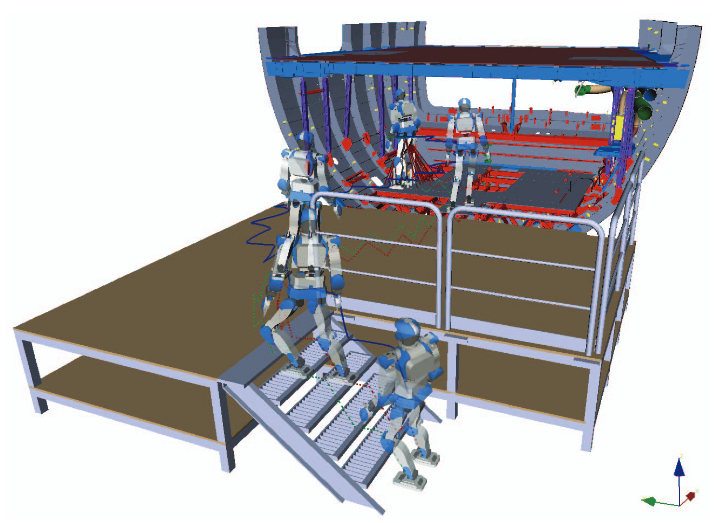
\includegraphics[width=\textwidth,height=5cm]{Figures/Chapter_INTRO/caron_image_plane.png}
        \caption{}
        \label{fig:intro_0}
    \end{subfigure}
    %\begin{subfigure}[t]{0.48\linewidth}
    %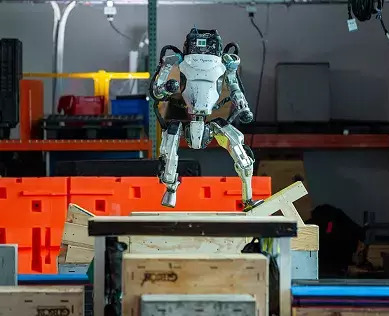
\includegraphics[width=\textwidth,height=5cm]{Figures/Chapter_INTRO/atlas_boston_dynamics.jpg}
    %\caption{\label{fig:intro_1}}
    %end{subfigure}
    \begin{subfigure}[t]{0.48\linewidth}
        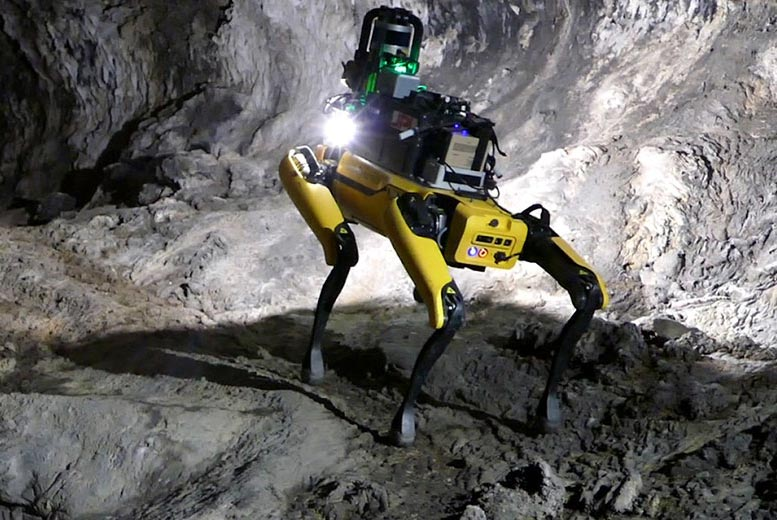
\includegraphics[width=\textwidth,height=4.5cm]{Figures/Chapter_INTRO/darpa_nasa.jpg}
        \caption{}
        \label{fig:intro_1}
    \end{subfigure}
    %\caption{Legged robots locomotion in complex environments. Sources: (a) \copyright Boston Dynamics and (b) \copyright NASA/JPL-Caltech.\label{fig:intro}}
    %\caption{Legged robots locomotion in complex environments. Sources: Caron et al. \cite{caron_plane_2016} and (b) ATLAS robot \copyright Boston Dynamics.\label{fig:intro}}
    \caption{Legged robots locomotion in complex environments. Sources: Caron et al. \cite{caron_plane_2016} and (b) \copyright NASA/JPL-Caltech.}
    \label{fig:intro}
\end{figure}

% TITLE: Reinforcement Learning of a Navigation Method for Contact Planning on Humanoid Robots


%    What is the problem?
%    Why is it interesting and important?
%    Why is it hard? (E.g., why do naive approaches fail?)
%    Why hasn't it been solved before? (Or, what's wrong with previous proposed solutions? How does mine differ?)
%    What are the key components of my approach and results? Also include any specific limitations. 

% https://www.futura-sciences.com/tech/actualites/robotique-interview-construire-robots-humanoides-90953/ : 
% Un des principaux intérêts motivant la construction de robots humanoïdes est sans doute sa compatibilité avec le monde des humains. Sans adaptation de notre environnement, ils pourraient vivre en harmonie avec nous au quotidien pour nous aider et utiliser nos infrastructures.

Robots are already essential tools in the industry and will play a part in our daily life in a near future.
However, most of them still require specifically designed environments to perform their task.
In recent years, research on legged robots has opened a whole new range of possibilities. %in primarily human-made environments.
These robots could operate in industrial areas to perform various tasks just like us, or explore in our stead risky environments (Figure \ref{fig:intro}).
Nevertheless, they have yet to perform the most basic but challenging skill that is to \textit{locomote through the environment}.

\section{Legged locomotion in complex environments}
% Je veux refaire le raisonnement de ce qu'un humain fait pour se mouvoir.
\begin{figure}[h]
    \centering
    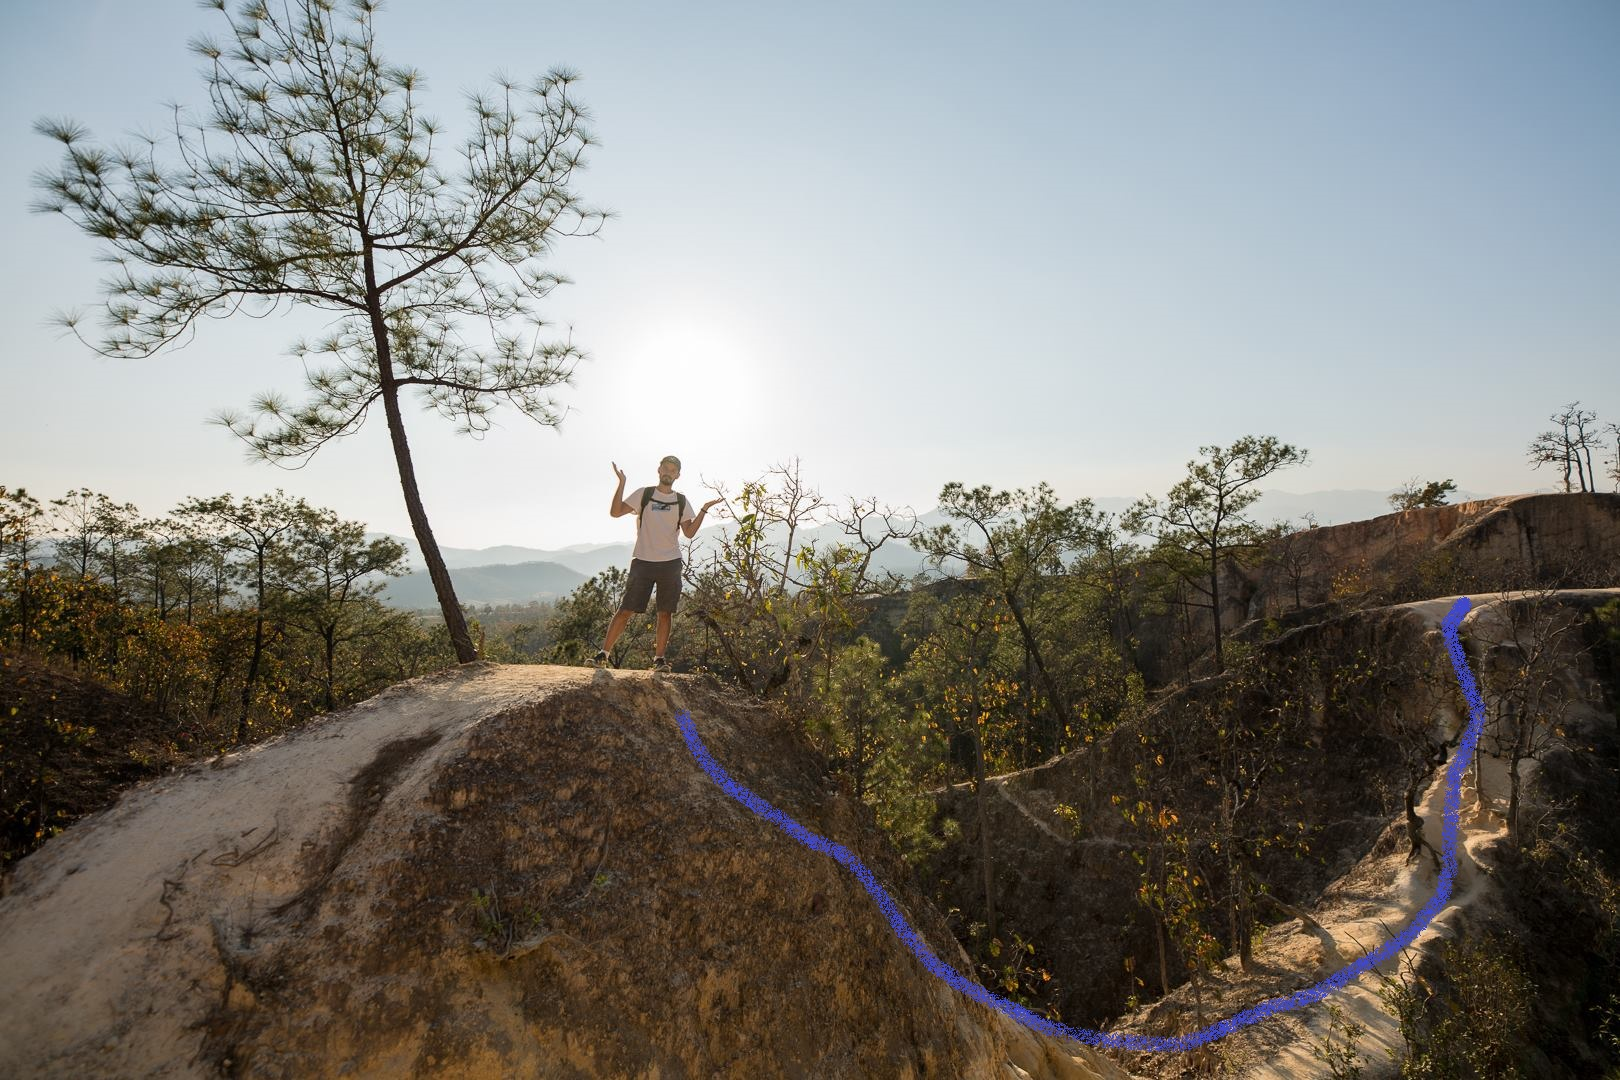
\includegraphics[width=\textwidth, height=8cm, trim={10cm 0 0 8cm}, clip]{Figures/Chapter_INTRO/moi_chemin.jpg}
    \caption{Planning the path and contacts is crucial to locomote on complex terrains.}
    \label{fig:intro:moi_chemin}
\end{figure}
In the large collection of works on legged robots, several strategies emerged to solve this problem.
In this thesis, we are interested in the robot locomotion problem in complex environments, that can be solved with a similar decision process to their creators.

We humans can achieve this task in real-time. 
As shown in Figure \ref{fig:intro:moi_chemin}, the objective is as follows: \qq{how to reach the other side of this terrain?}
Here, this task is particularly difficult, hence a thorough planning is required.
We can typically decompose this task into two sub-problems:
\begin{enumerate}
    \item \textit{What path do we take?} 
    This decision is based on an estimation of our capabilities. 
    First, the path is subject to conditions of \textit{reachability}, as we need to be able to touch the ground, and obviously of \textit{collision avoidance} as we can not go through obstacles.
    Second, we need to evaluate the terrain \textit{traversability} to plan a feasible path. 
    Based on these criteria, we decide to plan the blue path in our example.
    \item \textit{How do we move our body to follow the path?} 
    Walking without thinking where to place my foot could be sufficient for most scenarios. However, difficult terrains such as this one require a careful \textit{contact planning} to avoid taking a wrong step and falling.
\end{enumerate}
Human locomotion typically performs these two stages with (1) a navigation task to plan a feasible path, and (2) walking along this path while carefully planning our contact on the terrain.

Legged robot locomotion in general can employ the same strategy as demonstrated during the DARPA subterranean challenge \cite{darpa_nasa_2021, darpa_hutter_2022}.
In disaster scenarios, the robots have to map, navigate, and search for casualties in complex underground environments.

However, reproducing the masterful human reasoning for locomotion remains yet a difficult problem. How to program robots to achieve this decision process?
Furthermore, this decision process changes from individual to individual who continuously learns to estimate and improve their capabilities.



\section{Thesis Statement and Summary.}

This thesis if part of the Loco3D project \cite{loco3d} which goal is to achieve a fast to compute and safe solution for legged robot locomotion in complex environments.
In this context, we will further explored the use of a navigation task prior to contact planning on the terrain.
Our research topic is the critical limitation of this approach, that is the path feasibility by a contact planner.

Our main contribution is a local navigation method learned by reinforcement. 
Our method, named LEAS, can locally navigate under reachability and collision-avoidance constraints using a local observation of its environment.
During training time, LEAS can be plugged into a contact planner to learn how to generate more likely feasible paths for it, hence approximating its capabilities.
Finally, we will connect our navigation method with 3 different contact planners from the Loco3D project.

The organization of this thesis is as follows:

Chapter \ref{sec:sota} presents a review of the works on legged robot locomotion. 
We explore different solutions to obtain a safe and robust locomotion, leading us to our choice of a navigation method prior to contact planning (also known as the motion-before-contact approach). Finally, we present a general literature overview of the methods used in navigation that inspired our solution.

Chapter \ref{sec:LEAS} presents in-depth our steering method LEAS, that can locally navigate complex terrains.
We describe our method to learn by reinforcement how to generate paths under reachability and collision-avoidance constraints.
This chapter presents LEAS without being plugged to a contact planner, which is a local navigation task in 3D.

Chapter \ref{sec:CP-SB} presents the results of LEAS plugged into the acyclic sampling-based contact planner \cite{AcyclicCP}. 
Our steering method learns how to generate paths fitting this contact planner. 
As a result, it solves the compatibility problem we had with our previous solutions between navigation and contact planning.

Chapter \ref{sec:CP-SL1M} investigates the use of LEAS plugged into the Mixed-Integer Programming contact planner and its relaxation \cite{sl1m_v2}. 
We explain the formulations of these contact planners and their limitations relative to the guide. Finally, we present the results as well as the different experiments we conducted.

Chapter \ref{sec:conclusion} discusses the advantages and limitations of our steering method. Finally, we conclude with the perspective of this work.


\chapter{Background}
\label{sec:sota}
\minitoc
\bigskip

% Short intro
% Overview of what we explain in every subsection
Creating contact with the terrain is at the core of legged robots locomotion. 
%\stn{pas vraiment, dis plutot pourquoi ce st critique} \textcolor{blue}{?}
A large panel of methods has been proposed to achieve walking. 
Ranging from simple flat ground scenarios to more complex environments where planning is still challenging \cite{carpentier_survey_locomotion_robot}. 
%\stn{how challenging} \textcolor{blue}{Rajout de la phrase d'apres pour ca? Mais pas sur que ca soit mieux, ca reste une intro...} Indeed, it is a hard task to determine stable and feasible robot motion. 

%\stn{quel est l objectif de ce sota? dans les lignes qui suivent on va decrire qu il y a telle et telle approche, et justifier qu on est plutot dans cette approche. On va souligner le pb de cette approche et mettre en evidence le besoin de traiter de notre poblem P, pour lequel on testera l hypothese H}

In this thesis, we want a fast to compute and safe solution for the legged robot locomotion problem in complex environments.
To that end, we will explore the different strategies in the literature as follows:

\begin{itemize}
    \item Section \ref{sota1} reviews the contributions to achieve whole-body motion on legged characters and robots. The recent breakthroughs in Reinforcement Learning (RL) have yielded impressive results in the field of character locomotion, and more specifically contact agnostic approaches. However, these methods are inherently limited to low variations scenarios. In order to obtain a robust and stable walk in more complex scenarios, current works emphasize the need to plan contact positions.
    
    \item Section \ref{sota2} focuses on the contact planning problem, that is a common division of the locomotion task. We review two predominant contact planning strategies that are \textit{contact-before-motion}, that plans the contacts to be performed by a whole-body controller, and \textit{motion-before-contact}, that plans a rough robot base trajectory prior to contact planning along it.
    %This last strategy promises better computation performances alleviating the combinatorics of the contact planning problem, and relying on a trajectory planner to perform a navigation task.
    This last strategy relies on a navigation task to generate guide paths.
    
    \item Section \ref{sota3} is an overview of the works in navigation at two different scales, global and local. 
    Their goal is to generate conflict-free trajectories under different performance and optimality criteria in complex environments. %We then review two approaches of local planners, also called \textit{steering methods}.
    Finally, we see how these navigation planners can be used in the context of legged character locomotion.
    
    \item Section \ref{sota4} concludes this chapter with a summary of the different approaches to solve the locomotion problem. We show that dividing it into simpler subproblems such as whole-body control, contact planning, and navigation task is a promising solution for real-time locomotion on legged robots.
    Finally, we explain our choices and our problem formulation.
\end{itemize}




% ==== THE MAIN PROBLEM =====
% (P1+P2+P3) Too hard, too many dimensions, we do not know how to do.
% => Need contact planning.
% For dynamic walking, this is often done at the same time than the WBC because it's difficult to approximate it (hybrid solution), but for quasi-static it's ok.
% (P1+P2) How to do, it is a combinatorial problems. Some people like DEITS use a MIP or simplify the problem, others use a guide alleviate the combinatorics.
% (P1) We use some path planning algorithms (sampling-based) but a problem comes that is the feasibility of the guide with P2. We have some heuristics built empirically but overall, we do not know how to do.
% => Use Reinforcement Learning to learn how to do it.

% ==== Other problem ====
% Path planning is long to compute + the steering are often not terrain-aware, there are some works on navigation that could be helpful.

% ==== PLAN ====
% (P3 => P2)
% Explain the works on locomotion (P3) 
% Why we need contact planners (P2)
% Separate in two: 
% - contact-before-motion (most of the works)
% - motion-before-contact
% => P1
% In P1, there is path planning that have been searched extensively

\section{Synthesizing Locomotion \label{sota1}}
%\href{}{Link}\\
% Read well the related work of Ewen + RLOC
% P3 directly, on flat ok, on uneven we do not know (too big dim), lot of collisions, not suitable for biped. We need to specify the footstep location. (most works are in graphics for that, PPO paper etc). Then most of them relies on pre-defined footsteps to work.

% WBC aims to i) define a small set of simple, low-dimensional rules (e.g., equilibrium, self-collision avoidance, etc.) ii) that are sufficient to guarantee the correct execution of any single task, whenever feasible (e.g., reaching for an object with one end-effector), and of simultaneous multiple tasks (e.g., reaching for an object with one end-effector, while reaching for a second object with another end-effector), iii) exploiting the full capabilities of the entire body of redundant, floating-based robots in compliant multi-contact interaction with the environment.

% NICO SAYS BLABLA
%Locomotion of legged characters is a long-searched but still challenging topic.
%During its motion, the robot is constantly subject to dynamic constraints such as maintaining its equilibrium or avoiding collision of its body with the environment and itself.
%Its motion also has to be coordinated to perform a given task such as walking in a given direction or moving its feet to the next desired placement.
%The robot motion is performed by the \textit{whole body controllers}, which are among the most difficult controllers to engineer due to their numerous stability criteria \cite{Chevallereau_book, kajita_intro_humanoid_robotics}.

%In this section we classify the whole body controllers in two categories, namely \textit{contact agnostic} and \textit{contact-based} approaches.
%First, we review some contact agnostic works, that do not require (nor plan) the next contacts to perform with the environment. Those approaches have seen a lot of success recently with the use of RL algorithms for character locomotion.
%We then explore more classical and predominant contact-based approaches in the literature. 
%Those use predefined contact sequences or plan contacts with the environment during the motion simultaneously.

% Remarques nico:
% Definir le titre, methodes locales des premiers controlleurs de loco, fondees sur des lois de controle ou sur des principes d'optimalite permettant d'en obtenir.
% En quoi peut-on/doit-on les separer d'algo "planif" => Pas de recherche explicite de contact, eventuellement comme effet de bord du mouvement corps complet?
% Preciser: double grille de lecture
% - critere 1: decision de contact (imposee, guidee, libre, implicite)
% - Conformite du modele (Template LIPM, reduit, complet)
% Nous on choisit le critere 1 pour l'organisation des sections.

Research on modeling legged robot movements for locomotion is a long searched topic \cite{history_humanoid_robots}.
The task of determining stable and feasible motions is performed by the \textit{whole body controllers}. They are among the most difficult controllers to engineer due to their numerous stability criteria \cite{Chevallereau_book, kajita_intro_humanoid_robotics}.

Classical whole-body methods use control laws, which can be based on the principle of optimality. 
They do not explicitly search for contacts with the environment, and so naturally perform them as a side effect of the robot whole body movement.
As a result, these control approaches can be separated from \textit{planning} algorithms, that search for contacts or motions to be performed over a fixed horizon.
Two criteria to categorize these methods can be explored:
\begin{description}
   \item[(1) Contact decision,] that can be predefined, internal or free.
   \item[(2) Model complexity,] if the model is templated (e.g. Linear inverted pendulum model), reduced or complete.
\end{description}
This section is organized following criterion (1) based on the contact decision.

\subsection{Predefined Contacts}
\begin{figure}[h]
    \centering
    \captionsetup[subfigure]{justification=centering}
    \begin{subfigure}[t]{0.4\linewidth}
    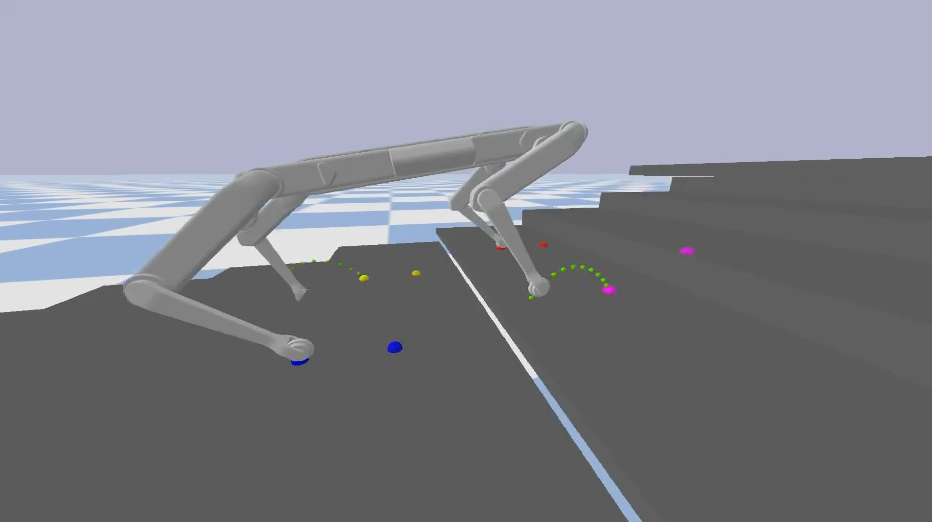
\includegraphics[width=\textwidth,height=4cm]{Figures/Chapter_SOTA//fanny_corbere_solo.png}
    \caption{Risbourg et al. \cite{fanny_mip_solo}}
    \label{fig:mpc_predefined_0}
    \end{subfigure}
    \begin{subfigure}[t]{0.58\linewidth}
    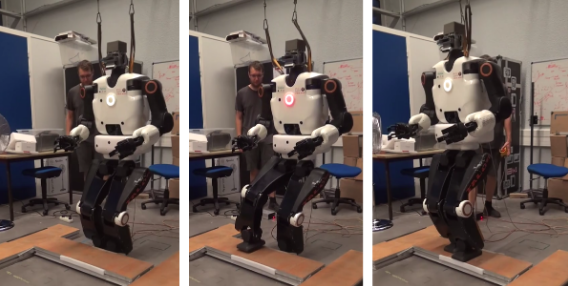
\includegraphics[width=\textwidth,height=4cm]{Figures/Chapter_SOTA//talos_ewen.png}
    \caption{Dantec et al. \cite{ewen_2022}}
    \label{fig:mpc_predefined_1}
    \end{subfigure}
    \label{fig:mpc_predefined}
    \caption{Whole body controllers performing predefined contacts.}
\end{figure}
Given a predefined sequence of contacts, efficient methods exist to compute the corresponding whole-body motion.
% Dynamics / Quasi-static
Knowing the dynamic state of the robot as well as its current and future contacts, approximation models can be used to plan the whole-body locomotion of legged characters.

\paragraph{Model-based approaches.}
Classical controllers of this category use the contact positions to compute either collision-free robot motion \cite{CHOMP_2009, stomp_2011, schulman_2014_collision, perrin_2012, fanny_mip_solo} (Figure \ref{fig:mpc_predefined_0}), or the centroidal dynamics of the robot to achieve locomotion \cite{hauser_prm_motion_planning_2005, lin_motion_planning_2016, prete_featherstone_2017, caron_2018_whole_body, Tonneau2018_2PAC}.
In the seminal work, Kajita et al. \cite{kajita2003ZMP} introduce a walking pattern generator, using the zero moment point and the inverted pendulum mode, that allows arbitrary foot placements.
%\stn{pkoi c est dans predefined contacts => Kajita 2003 = ZMP pour le stepping stone problem.} 
They then demonstrate the efficacy of their controller climbing some stairs with a humanoid robot in simulation.
From a contact sequence, some works \cite{carpentier2016_versatile_efficient, pierre_alexandre_2021} use a model-predictive controller to compute a stable trajectory for the Center of Mass, coupled with a whole-body controller.
%In the same fashion, Leziart et al. \cite{pierre_alexandre_2021} use a centroidal model predictive control to compute the contact forces that should be applied by a quadruped robot on the ground.
With a different approach, Dantec et al. \cite{ewen_2022} propose a whole-body model predictive control to follow predefined footstep on the torque-controlled humanoid robot Talos \cite{talos_robot} (Figure \ref{fig:mpc_predefined_1}).

\paragraph{Learning whole-body controllers.}
Such controllers can also be learned by reinforcement in simulation \cite{ALLSTEPS_2020}.
Peng et al. \cite{deepLoco} train a biped character in simulation to follow predefined footsteps, and achieve walking in mostly flat environments.
Following this idea, Tsounis et al. \cite{deepGait} learn a whole-body controller in simulation for quadruped locomotion on more complex terrains. 
Gangapurwala et al. \cite{RLOC} learn whole-body motion tracking and recovery controllers for improved robustness, accounting for changes in the dynamics of the robot and perturbations. Their policy is then performed on a real quadruped robot.
Combining model-based and RL approaches, Xie et al. \cite{glide_xie_2021} learn by reinforcement how to control the accelerations of a centroidal model, then used to compute ground reaction forces translated to joint torques applied on the robot.
Their method, combined with simple heuristics for footstep placement, demonstrates robust walking in complex scenes on the quadruped robot Laikago. %\textcolor{blue}{Is glide set in the right section ? For me yes.}

To these days, such controllers are mostly applied in real-world to quadruped robots and have yet to be performed on humanoid robots \cite{papier_rohan_wbc_rl_2022}.

\paragraph{Conclusion on predefined contacts.}
Most of the works in the literature focus on whole-body controllers generating motions over predefined contact sequences.
Model-based approaches have shown impressive locomotion skills on complex environments \cite{ladder_robot_2}.
Reinforcement learning is another approach to obtain such controllers. 
The trained controllers can cope with the system dynamics along with stability criteria. 
However, they require up to several days of training, and are yet to achieve the results of model-based controllers on real humanoid robots.


\subsection{Internal Contact Decision}
%\textcolor{blue}{Avant "Explicit contact decision", j'aime pas trop le terme parce qu'au dessus c'est aussi explicite. Si c'est calcule en interne par le WBC... j'ai mis internal?}
\begin{figure}[h]
    \centering
    \captionsetup[subfigure]{justification=centering}
    \begin{subfigure}[t]{0.30\linewidth}
    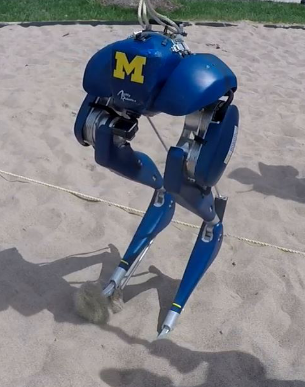
\includegraphics[width=\textwidth,height=4.5cm]{Figures/Chapter_SOTA//cassie_walking_sand.png}
    \caption{Gong et al. \cite{Cassie_feedback_control_2018}\label{fig:walking_task_0}}
    \end{subfigure}
    \begin{subfigure}[t]{0.45\linewidth}
    %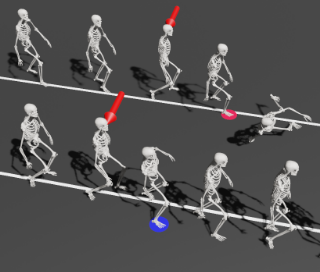
\includegraphics[width=\textwidth,height=4.5cm]{Figures/Chapter_SOTA//hwangpil_biped_stability.png}
    %\caption{Park et al. \cite{hwangpil_stable_2020} }
    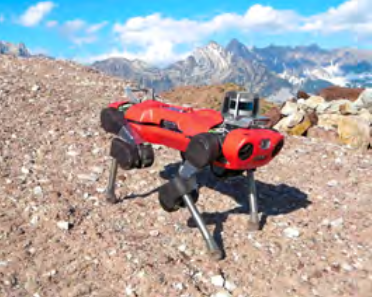
\includegraphics[width=\textwidth,height=4.5cm]{Figures/Chapter_SOTA//anymal.png}
    \caption{Lee et al. \cite{hutter_challenging_terrain}\label{fig:walking_task_1}}
    \end{subfigure}
    \caption{Legged robots walking on small variation terrains.\label{fig:walking_task}}
\end{figure}

%Whole-body controllers can also compute the contacts internally along with the robot motion.

\paragraph{Flat floor.}
%\textcolor{blue}{To modify?}
Traditional whole-body controllers for flat ground locomotion make the assumption that contacts will always occur at the same height in global space.
Achieving stable, periodic walking on flat ground is already a challenging problem in itself to comprehend the nature of dynamic models for locomotion, which is especially difficult for biped robots \cite{grizzle_chevallereau_2010}.
The study of the center of mass trajectory, with the linear inverted pendulum model and zero moment point as well as their variations, has been at the core of the legged locomotion problem with model-based approaches.

%\textcolor{blue}{What I say bellow for chevallereau + tsujita has to be rechecked. I am not confident in this part on model-based WBC.}
A common strategy to solve this problem is to use a reference walking motion, which is then modified by the whole-body controller to ensure its stability at runtime.
Using such a controller, Chevallereau et al. \cite{Chevallereau_2008_zmp} modify the reference joint motion to obtain the desired zero moment point evolution, and thus a stable walking motion.
%modify a reference motion in order to ensure a stable motion. (e.g. model predictive control), mostly using the so called Zero Moment Point (ZMP) \cite{zmp_history}, and low level controller tracking this reference motion (e.g. feedback control).
Tsujita et al. \cite{gait_pattern_2001} propose a gait pattern controller adapting the reference motion in function of touch sensor signals on the foot of a quadruped robot. % They use a non-linear oscillator to have a nominal ref motion that is modified in function of the touch sensors.

% Using simplified models (as winkler 2018 says)
Simplified models of robot dynamics are an effective strategy.
Using a linear inverted pendulum as a reduced model of the robot, Kajita et al. \cite{kajita2002LIP2} propose a real-time walking pattern generator that adapts footsteps during the motion to follow a desired walking speed and direction.
% They optimize CoM - CoP - Footstep simultaneously.
In this line of work, Herdt et al. \cite{herd_2010, herd_perrin_2010} introduce the notion of \qq{walking without thinking}, where a model predictive control scheme takes as input a given direction to follow, and outputs safe foot placements and motion to walk seamlessly while reacting to disturbances on the humanoid robots HRP2.
% Other task inside the MPC => Footstep plan in function
Such a strategy permits fast online planning \cite{hurst_2018} as well as the optimization of different tasks simultaneously such as locomotion and manipulation \cite{florent2012} or obstacle-avoidance in real-time \cite{naveau2017}.
%However, these approaches are mostly limited to flat grounds due to their formulation.
%A limitation of these controllers is that they are by nature short horizon planner that would be prone to local minima on more complex scenarios (where the robot motion gets trapped in a loop and is not able to go forward). \textcolor{blue}{Is my definition ok or I'm totally wrong}


\paragraph{Small variation terrains.\label{par:whole-body:uneven}}
Another strategy is to consider a nominal reference motion on flat ground, then make it robust enough to be performed on complex terrains.

It can be bone by simplifying the robot dynamics model with the linear inverted pendulum model to generate a nominal reference motion considering a flat ground.
This motion is then performed by the whole body controller that adapt it for complex and rough terrains.
Rezazadeh et al. \cite{rezazadeh_hurst_atrias_2020} include a reflex-based control scheme to walk blindly on uneven terrain with the biped robot Atrias.
Building upon this work, Gong et al. \cite{Cassie_feedback_control_2018} adapt motions from a gait library and demonstrate various locomotion tasks on the biped robot Cassie including walking in the sand (Figure \ref{fig:walking_task_0}) or balancing on uneven moving surfaces.

Learning a controller from data can produce natural and plausible walking motion \cite{learned_motion_matching, pfnn}.
However, data-driven strategies often require a large amount of motion capture data, and can not cope with the dynamics variations in the robot (or character) states inherent to physics-based simulations and the real world.
Reinforcement learning, and more specifically imitation learning, can overcome this limitation and bridge the gap between simulation and reality (sim-to-real).
Li et al. \cite{CassieLi2021} learn to adapt motion from a gait library. 
They then achieve the sim-to-real by randomizing the system dynamics in simulation, and achieve robust locomotion on the biped robot Cassie.
% Hutter => Quadruped in the nature.
Using another strategy, Lee et al. \cite{hutter_challenging_terrain} learn a teacher policy for walking on the quadruped robot ANYmal, that is fully aware of its surrounding environment.
The safe motion generated by the teacher is then imitated by another policy, that learns how to blindly walk in complex terrains.
They then demonstrate walking in the real world in very rough scenarios (Figure \ref{fig:walking_task_1}).
% Residual
Learning residual control is another method to bridge the reality gap. Duan et al. \cite{residual_rl_cassie_2021} directly learn how to modify the reference motion with residual actions to obtain a more robust bipedal walking.

While these works demonstrated the capabilities of their whole-body controller to walk in uneven terrains, they remain limited in more complex scenarios. Indeed, they are performing a control in reaction to impacts on the environment. As a consequence, they are irremediably prone to collisions (and falls) on terrains such as stairs.

\paragraph{Simultaneous motion and contact optimization.\label{par:simul_contact_motion}}
%\stn{reprends la structure du sota du journal de daeun, elle est tres bien pour differencier les 2. Tu dois surtout expliquer la logique. Le truc clef c est pas la taille du modele. C est de dire on smooth un pb discret en un probleme continu. Les papiers se situent par rapport a cette frontiere. Tu dois mettre ca en chapeau. Les premiers papiers en ont pas besoin parce qu hyothese simpificatrice, les autres si. Donc c est ca ta distinction: comment tu formule le contact de maniere continu. Soit en reduisant l espace de recherche, soit en lissant la dynamique}
%\textcolor{blue}{Je suis dans la section des whole body controller. Parler de la difference entre continue/discrete approches pour la selection des surfaces/contacts n'est peut etre pas le bon endroit?}

Optimizing simultaneously contact and motion permits the consideration of the robot dynamics in the contact choice, considering a known terrain model.

% It's planning => offline and long, but this time we can consider the terrain and optimize everything.
% Mordatch 2012
% Carlos 2017
% Carlos 2020
% Winkler + hutter 2018 (MIP for the whole stuff)
% Ponton 2020 (same on SOLO, check the diff)
Approximating the environment as a continuous function and computing contact and motion permits the generation of whole-body motion in complex terrains \cite{Dai_2014, posa2014}.
In simulation, Mordatch et al \cite{mordatch2012DiscCIopt} present a contact invariant method optimizing contacts and motion trajectory simultaneously to perform a wide variety of locomotion tasks.
In the same line of work, Winkler et al \cite{winkler2018GaitOpt} present a trajectory optimization formulation generating highly dynamic motion plans for a variety of legged characters on complex terrains.
Whole-body trajectory optimization was successfully applied to real quadruped robots, achieving planning on flat ground and execution of walking movements in near real-time \cite{Winkler2017_TO}.

Mixed Integer Programming (MIP) formulation can be used to solve the discrete choice of the next contact surface selection and continuous optimization of the motion, extending this method for quadruped locomotion to uneven terrains \cite{carlos_2019}.

Trajectory optimization of simplified or full dynamics model is promising to perform safe and robust locomotion, benefiting from the contact-based approach as well as considering the dynamic state of the robot in the planning as well as the terrain constraints.
However, as the size of the model used and the complexity of the terrain increase, this approach suffers from high computation time (up to several seconds per footstep), limiting its application for real-time planning. 
Some promising works solve this limitation \cite{ponton_righetti_2020, hutter_last_work_nmpc}, but they rely on a separate planner to find the next contact surface to step on.

\paragraph{Conclusion on internal contact decision.}
A classical approach for locomotion is to synthesize walking motion while adapting footstep placement on flat ground.
Generalizing these approaches to uneven terrains is feasible but limited, as such controllers consider the terrain variations as errors during the motion that need to be fixed.
Finally, trajectory optimization is promising to plan safe walking motion on complex terrains. However, these methods are still expensive to compute.

\subsection{Contact Agnostic}
Whole-body controllers previously presented implicitly or explicitly reason about contact placement on the terrain.
Another strategy is to employ a contact agnostic approach, where the controllers are not given any reference motion, or contact sequence, and are provided with little to no info about the terrain.
%They have to answer the following question: \textit{can we generate walking motion without reasoning about contact placements on the terrain?}

%These approaches typically uses sensor datas of the robot to estimate its stability.
%Previous works presented in Section \ref{par:whole-body:uneven} answers the question considering a walking motion on flat ground and relying on the robustness of their whole-body controller to adapt to more complex terrains. However, the expected walking motion implies to reason about contact placement to a certain extension.

%This section is an informational overview of works on locomotion with a contact agnostic approach.

\paragraph{Learning how to locomote.}
% First I talk how in graphics they used to simulation locomotion (kinematics).
% MOVED TO UNEVEN TERRAINS
%In a purely kinematic simulation, learning a controller from data has long been used to produce a natural and plausible walking motion \cite{learned_motion_matching, pfnn}.
%Given a some motion capture datas, the control policy finds the most suitable motion to perform in function of its situation and a user control. In these approaches, the next foot position is computed directly from the chosen motion, transposing its location on the terrain.
%Such control from data is traditionally done by building a motion graph and selecting the next motion to perform \cite{Kovar2002, jehee_lee_2002, jehee_lee_2006, motion_matching}. 
% Then how machine learning helped for that (PFNN etc).
%To cope with the huge amount of data available, recent works in machine learning have shown impressive results to synthesize character motion replacing graphs by neural networks \cite{learned_motion_matching, learning_predict_rnn}. 
%Learning a policy mapping user input and gait of motion with a motion database, Holden et al. produce a natural locomotion on bipedal character over uneven terrains \cite{pfnn}, later extended to quadruped \cite{pfnn_wolf}.
% But it's all in kinematic and can not cope with the dynamics of the system.
% MOVES TO UNEVEN TERRAINS
%However, data-driven strategies often require a large amount of motion capture data and can not adapt to the dynamics variations in the robot (or character) states inherent to physics-based simulations and the real world.
%\textcolor{blue}{I am not sure if talking about ML approach is pertinent. Let's see if it's too much at the end. I'll just have to remove everything above in this paragraph and keep only RL (bellow).}
\begin{figure}[h]
    \centering
    \captionsetup[subfigure]{justification=centering}
    \begin{subfigure}[t]{0.36\linewidth}
    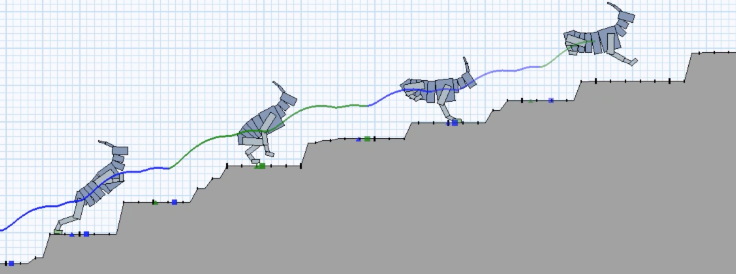
\includegraphics[width=\textwidth,height=3cm]{Figures/Chapter_SOTA//terrain_adaptive.png}
    \caption{Peng et al. \cite{terrain_adaptative_locomotion}}
    \label{fig:rl_agnostic_0}
    \end{subfigure}
    \begin{subfigure}[t]{0.36\linewidth}
    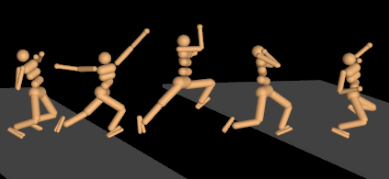
\includegraphics[width=\textwidth,height=3cm]{Figures/Chapter_SOTA//deepMindPPO.png}
    \caption{Heess et al. \cite{ppo_rich_locomotion} }
    \label{fig:rl_agnostic_1}
    \end{subfigure}
    \begin{subfigure}[t]{0.25\linewidth}
    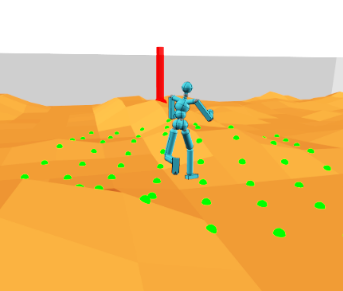
\includegraphics[width=\textwidth,height=3cm]{Figures/Chapter_SOTA//vae2.png}
    \caption{Won et al. \cite{VAE_jungdam_2022}}
    \label{fig:rl_agnostic_2}
    \end{subfigure}
    \label{fig:rl_agnostic}
    \caption{Works on reinforcement learning for legged characters locomotion.}
\end{figure}

% That is where Reinforcement Learning becomes really useful in physics-based sim.
Reinforcement Learning (RL) in physics-based simulation can be used for character animation \cite{survey_rl_animation_pettre_2022, won2017dragon, seheeOctopus2019, learning_predict_rnn}.
This method permits learning controllers able to cope with the system dynamics.
They offer better generalization capabilities to new environments or unexpected events compared to traditional model-based approaches that are highly complex to engineer. 
Peng et al. learn by reinforcement a terrain-adaptive locomotion controller, outputting target joint angles to compute the torques on 2D biped and quadruped characters \cite{terrain_adaptative_locomotion} (Figure \ref{fig:rl_agnostic_0}). 
Using a similar control, such RL controller can be extended to 3D locomotion \cite{ppo_rich_locomotion} (Figure \ref{fig:rl_agnostic_1}).
%for example using Proximal Policy Optimization (PPO) RL algorithm \cite{PPO_2017}.
These seminal works are the basis of many others further improving the naturalness and robustness of the motions as well as the diversity of skills performed \cite{drecon, carl, Lee_muscles_rl_2019}.
More recently, Won et al. \cite{VAE_jungdam_2022} use conditional variational autoencoders to learn how to imitate motion from a database and achieve various tasks in a physics-based simulation. 
One of their results shows a biped locomotion task using a low-resolution local height map as terrain observation to walk and run on rough terrains.

Evolutionary algorithms can be a suitable alternative to RL, even to learn locomotion skills from scratch \cite{evol_vs_rl_deepmind_2017}. 
While both approaches present their pros and cons \cite{evol_vs_rl_majid_2021}, they also present similarities as they both learn from interactions with the environment.
Covariance matrix adaptation is one evolution strategy that can be used to learn walking by controlling torques \cite{yin_simbicon_2007, wang2009} or musculo-tendon units on humanoid characters \cite{wang2012} and various biped creatures \cite{van_de_panne_2013}.

% Mini conclusion
The recent breakthroughs in RL algorithms such as PPO \cite{PPO_2017} and others \cite{TD3_2018, SAC_2018} have permitted the learning of highly adaptive whole-body controllers on rough terrains for legged character locomotion in simulation.
% Very promising alternative to model-based, but not very stable
These methods are promising to compensate for the weaknesses of model-based approaches, which can be difficult to develop and demonstrate fewer generalization capabilities.
However, these controllers are often long to train as they require millions of interactions with the environment. Moreover, the motions generated are usually jerky visually, and the search for a more stable bipedal walk with RL remains \cite{hwangpil_stable_2020}.
%Finally, some works show that acting in task space (e.g. proportional derivative control) \cite{does_choice_action_space_peng_2016} and leveraging the knowledge of traditional model-based controllers is promising to learn controllers faster, while producing more robust behaviors.

\paragraph{Robot learning and sim-to-real.}
% But as said previously, the fidelity of the simulation compared to the real world is not good.
Several works using RL demonstrate how to learn to walk on legged characters under a few hours in simulation.
However as stated in the survey of Ibarz et al. \cite{survey_sergey_robot_rl}, a policy learned in simulation usually performs badly on the real robot due to the discrepancy between the simulation and the real world.

% Sim-to-real methods
Diverse sim-to-real methods have appeared to bridge the reality gap such as randomizing the simulation dynamics \cite{peng_domain_randomization_2017}, identifying the dynamics parameters on the real robot \cite{liu_sim_to_real_2019} or developing an accurate actuator model and simulating latency \cite{sim_to_real_agile_2018}.
% This has been moved to Uneven terrains.
%Li et al. \cite{CassieLi2021} randomize the dynamics of the system in the simulation using \cite{peng_domain_randomization_2017} and learn to imitate motions from a gait library in simulation, to then achieve robust locomotion on a real biped robot.
% Hutter => Quadruped in the nature.
%Lee et al. \cite{hutter_challenging_terrain} learn a teacher policy fully aware of the robot surrounding environment to teach another policy how to perform a robust blind quadrupedal locomotion in simulation, then demonstrate walking in very rough scenarios (Figure \ref{fig:rl_agnostic_robot_1}).
While those methods alleviate the reality gap problem, they do not compensate totally for the environment model inaccuracy in simulation. 
That is why such trained controllers could require additional fine-tuning on the real robot.

\textcolor{blue}{C'est le papier de mouret avec l'araignee. Ils utilisent des evol algo pour trouver une strategie de marche qui fonctionne sur le robot. Il essaie plusieurs strat et trouve la meilleure dans une map qui fonctionne. Donc il peut s'adapter au monde reel. La phrase d'en dessous c'est peut etre pas adaptee.}
To alleviate this gap, some strategies can also quickly adapt to the real-world.
% Mouret with robot that can adapt like animal => Hard to place
Mouret et al. \cite{Mouret_adapt_like_animals_2014} learn a behavior-performance map using evolutionary algorithms to achieve locomotion on a small hexapod robot in function of its limb damages. Their robot is then able to adapt its behavior online to walk even when damaged.

\paragraph{Robot learning in the real world.}
\begin{figure}[t]
    \centering
    \captionsetup[subfigure]{justification=centering}
    \begin{subfigure}[t]{0.48\linewidth}
    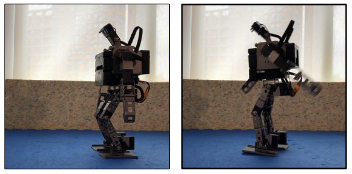
\includegraphics[width=\textwidth,height=4cm]{Figures/Chapter_SOTA//heess_robot.png}
    \caption{Bloesch et al. \cite{rl_wild_heess_2022}}
    \label{fig:rl_agnostic_robot_0}
    \end{subfigure}
    \begin{subfigure}[t]{0.4\linewidth}
    %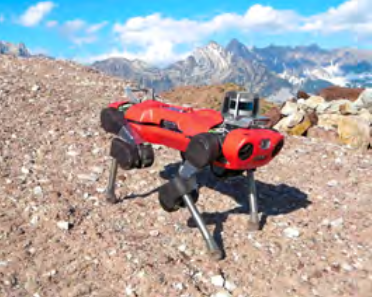
\includegraphics[width=\textwidth,height=4cm]{Figures/Chapter_SOTA//anymal.png}
    %\caption{Lee et al. \cite{hutter_challenging_terrain}\label{fig:rl_agnostic_robot_1}}
    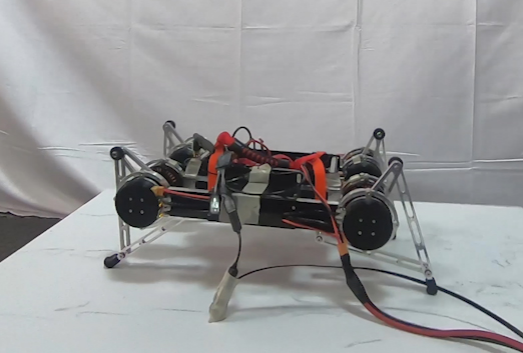
\includegraphics[width=\textwidth,height=4cm]{Figures/Chapter_SOTA//sergey_rl.png}
    \caption{Haarnoja et al. \cite{sergey_2018}}
    \label{fig:rl_agnostic_robot_1}
    \end{subfigure}
    \caption{Robots learning how to walk in the real world.}
    \label{fig:rl_agnostic_robot}
\end{figure}
% What's the challenge in robotics
% We do not want to break the robot => No collision if possible, no strong impacts, jerky movements lead to dynamics instability making the robot fall or collide so we need to avoid it.
Learning controllers by reinforcement directly on real robots is a promising direction to remove the dependency on imperfect simulation \cite{rl_robotics_survey_2013}.
However, such an approach is challenging due to critical real-world limitations.

The sampling collection is a tedious process on the real robot, and so the policy has to be learned from a significantly less amount of data. As a consequence, algorithms with better sample efficiency are required \cite{sergey_2018, calinon_micro_rl}.

Reinforcement learning algorithms are trial-and-error processes, thus leading to numerous failures during learning. 
In the real world, these failures translate into a high risk of breaking the robot and a potential threat to the safety of its surroundings.
% Some attempts to learn directly on the real robot with RL (spider etc).
As a result, learning whole body controllers \qq{in the wild} \cite{rl_wild_heess_2022}, meaning directly on the real robot, requires additional safety measures.
% Talk first about RL directly on the robot: quadruped (Sergey Levine 2019) + Towards General and Autonomous Learning (Hafner 2020)
Most works on the topic avoid such an issue by learning on relatively small-sized and harmless robots \cite{nao_rl_world_docking, rl_wild_heess_2022}. 
Back in 2005, Tedrake et al. learn how to walk by reinforcement directly on a low degree of freedom biped robot \cite{tedrake2005learning}. 
Later on, as the RL algorithms and robot designs improved, learning locomotion from scratch has been performed on quadruped \cite{sergey_2018} (Figure \ref{fig:rl_agnostic_robot_1}), hexapod \cite{deepmind_locomotion_RL} and more complex biped robot \cite{rl_wild_heess_2022} (Figure \ref{fig:rl_agnostic_robot_0}).
Another limitation of learning in the real world is that during the training (up to several hours or days), the human will have to manually reset the robot position as it falls over, bumps into a wall, or reaches the edge of the terrain.
% Safety: recovery policy (Tan 2022)
Yang et al. \cite{yang2022safe} alleviate this limitation by lowering the number of falls. They propose a safe recovery policy to take over the control when the learning agent violates some safety constraints, thus decreasing the need for human intervention while improving the safety of the robot.

% But it's long and high risk to break the robot => Still a research topics and not feasible at all on biped for now.
Applying RL in the wild is an exciting research direction. But it is for now limited in the context of locomotion to small robots that require constant human intervention during training, and which has only been applied to flat ground so far.
Designing bigger-sized robust robots or strategies to make the robot automatically recover \cite{leo_robot_2010} are promising directions.

\paragraph{Conclusion on contact agnostic approaches.}
%Classical model-based controllers have been extensively studied over the past years to achieve blind walking \cite{Cassie_feedback_control_2018}.
%However, those are complex to engineer as they require some good models of the robot and dynamics, and can lack the ability to adapt to unexpected variations in the environment due to their constant uncertainty about the position of the next contact. 
% So the safest way is to learn in simulation then pass it in simulation => Sim-to-real problem.
The recent surge in the use of reinforcement learning has proven promising to develop controllers with a contact agnostic approach.
Works on this topic demonstrated impressive results to generate robust walking motion, while adapting to the rough terrains in simulation \cite{VAE_jungdam_2022} and in the real world \cite{yang2022safe}.

Nowadays, learning robot locomotion (and other skills) in the wild is yet limited to small robots for safety and cost reasons.
Learning from simulation remains the best way to ensure the safety of the robot and its surroundings.
It also permits to easily reset the robot state, and bypass the poor data efficiency of learning on real systems \cite{atrias_rl_sim_to_real} (i.e. tedious collection process of data). 
However, learning a safe and robust walking on biped robots without specifying a reference motion or contacts is still difficult.
Finally, the search for more accurate simulations or efficient sim-to-real methods remains.

%Furthermore, contact agnostic approaches are inherently limited due to their blind nature which irremediably leads to a high number of collisions in more complex environments as well as potentially strong impacts on the terrain.
%These limitations put at risk the robot and its surrounding, which we can not afford on costly big-sized robots.


\subsection{Conclusion}
% Conclusion: On a des methodes qui existent pour generer le whole body motion pour des pas donnees (s'ils sont faisables). D'autres methodes essaient de generer ou replannifier ces pas en meme temps que le whole body motion, mais ont des temps de calcul vraiment enorme ce qui n'est pas possible pour du online-replannning sur le vrai robot. 
% Comme on veut un temps de calcul rapide <<1mn, on doit donc utiliser des pas predefinis en amont de la whole body locomotion, c'est a dire faire du Contact Planning. 
% Cette hierarchical decomposition rend le probleme plus facile a traiter.

%Whole body controllers with a contact agnostic approach are complex to engineer. 
%Their blind nature allows them to detect contacts with the terrains only after the impact. In spite of few successes with traditional model-based and more recently RL controllers, they remain limited to low variations grounds and can not be applied to more complex terrains without guarantee of safety for the robot. \textcolor{blue}{Safety may not be the right word?}
% Say that it's blur
%It is important to note that contact agnostic controllers still consider contact placements to some extent. 
%Indeed, a blind controller will somehow expect the next contact to be at a fixed position on flat ground and adapt as best its control in function of its sensors measurement.

%Accurately defining contact position is essential to obtain a stable and safe locomotion behavior.
%Methods optimizing the motion and the contact position simultaneously permit to obtain of dynamic motions, but are not yet real-time capable due to the high dimension of the problem solved.
%Whole-body controllers to perform a predefined sequence of footsteps have been extensively studied in the literature, and several of them do this task efficiently \cite{carpentier2016_versatile_efficient, pierre_alexandre_2021, ewen_2022}.

%In order to get a safe and fast to compute locomotion planner, working with predefined contacts remains the most efficient strategy.
%Now we are left with one question: \textit{How to obtain these contacts ?}
%Manually defining those is a solution for fixed scenarios, but to obtain a more general locomotion planner we need to investigate the so-called \textit{contact planning problem}.

% Nicolas: 
% Real interest for contact agnostic, but not feasible yet.
% Explicit contact decision: limited to flat ground, and when applied to more complex terrains => Not stable/collision or too expensive to compute.
% As a result, to fastest and prefered solution to generate a walking motion is still to rely on a prior contact decision. This contact sequence can be given by the user, but we desire to automatize this task. So we have to see the contact planning.
Research in locomotion has seen a lot of interest in contact agnostic approaches using reinforcement learning.
However, these methods are not mature yet to be feasible on a real human-sized robot.

Contact decision is thus still required to generate a safe and robust walking motion.
Implicitly optimizing the contact position along with the motion are mostly limited to flat ground scenarios.
While recent whole-body controllers can demonstrate good generalization to uneven terrains, they are still inherently limited due to their blind nature.
Simultaneous motion and contact optimization are promising to generate dynamic and safe locomotion. 
However, they remain expensive to compute, thus limiting their use for online planning.

Following predefined contacts is still the most efficient way to synthesize locomotion. 
To that end, efficient whole-body controllers exist to perform this task \cite{carpentier2016_versatile_efficient, pierre_alexandre_2021, ewen_2022}.
Now we are left with one question: \textit{How to obtain these contacts ?}
Manually defining them is a solution for fixed scenarios, but to obtain a more general locomotion planner we need to investigate the so-called \textit{contact planning problem}.


% ===============================================================================


\section{The Contact Planning Problem \label{sota2}}

% Was made a nice choice because of the improvements in approx of feasiblity (CROC) for example.

% - 2 - Contact planning
% We need to plan contact for biped locomotion. The decoupling of whole body motion and footstep planning is faster but raise another problem that is the feasibility of the plan by the WBC, all mostly solved by the state of the art contact planners available. Separated in two families:
% Contact-before-motion: most of the works with many different strategies. Consist in searching the best foosteps to perform among all surfaces, subject to a combinatorial problem when planning several steps ahead.
% Motion-before-contact: A lot less know, consists in computing a rough root trajectory for the root of the robot (motion) before computing the contacts relative to this trajectory. This method constraints the exploration of the combinatorics of the contact planning only along this root trajectory, alleviating the combinatorics probem.

A contact planner finds a sequence of contact positions that the robot has to perform to go through the terrain.

As stated by Chestnutt et al. \cite{chestnutt_2009_interactive_guide}, planning footsteps rather than whole body motion allows the robot to reason about contact with the environment to ensure safe and stable support. This also reduces the planning state space to a dimensionality computationally tractable for online walking.
From a sequence of predefined contacts, efficient whole body controllers exist for motion planning \cite{carpentier2016_versatile_efficient, caron_2018_whole_body, pierre_alexandre_2021, ewen_2022}.
The division of whole-body control and contact planning greatly lowers the complexity of the locomotion problem. Indeed, it relies on simplifications and assumptions on the robot dynamics to efficiently compute a feasible sequence of contacts.
However, it also comes at the cost of the non-guarantee of the feasibility of the contact plans. This limitation is avoided by previously presented methods which compute motion and contacts simultaneously \cite{Winkler2017_TO, carlos_2019}.

In this section, we classify contact planners of the literature into two categories as described by Bretl et al. \cite{bretl2006}:
\begin{itemize}
    \item \textit{contact-before-motion}, that decides the future contact placements, before planning the whole body motion.
    \item \textit{motion-before-contact}, that further divides the contact planning into two sub-problems. First plan a rough trajectory the robot root has to follow, which we call the \textit{guide path}, then compute the contact placement along it, and finally the whole-body motion.
\end{itemize}
We will explore the results of both strategies, along with their pros and cons.

\subsection{Contact-before-motion\label{subsub:contact-before-motion}}
\begin{figure}[t]
    \centering
    \captionsetup[subfigure]{justification=centering}
    \begin{subfigure}[t]{0.48\linewidth}
    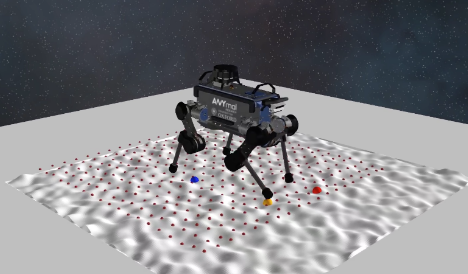
\includegraphics[width=\textwidth,height=4cm]{Figures/Chapter_SOTA//rloc_planning.png}
    \caption{Gangapurwala et al. \cite{RLOC}}
    \label{fig:cp_bm_0}
    \end{subfigure}
    \begin{subfigure}[t]{0.48\linewidth}
    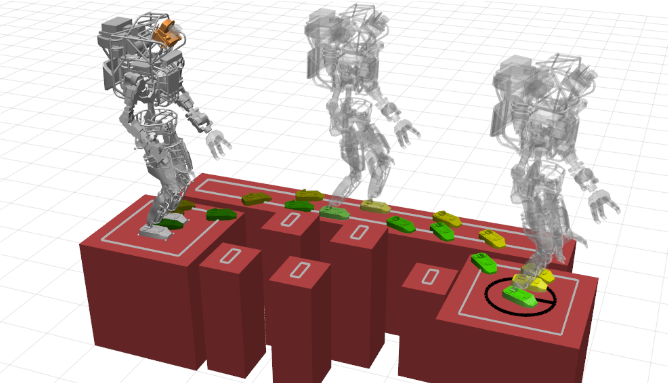
\includegraphics[width=\textwidth,height=4cm]{Figures/Chapter_SOTA//MIP_deits.png}
    \caption{Deits et al. \cite{deits2014FootPlanMI}}
    \label{fig:cp_bm_1}
    \end{subfigure}
    \label{fig:cp_bm}
    \caption{Contact-before-motion strategy with (a) short horizon and (b) long horizon planning.}
\end{figure}

%\textcolor{blue}{Fanny proposait de mettre cette section apres: Expliquer d'abord comment on place les contacts, ensuite comment on verifie s'ils sont valides. Moi je propose l'inverse, comment on verifie si un contact est valide, et ensuite comment a partir de ca on planifie. Quel ordre serait le mieux?} 
%\stn{a ce stade le schema de ma these aurait vraiment ete utilise qqe part}
Planning contact placements prior to the whole-body motion raises a key problem: \textit{how to know if a sequence of contacts is feasible by the robot?}
% Explanation
Seminal works solve this question using simplified models of the robot dynamics in its environment. Their related concepts such as the zero momentum point \cite{kajita2003ZMP} or contact wrench cones \cite{trinkle_2002_cwc} can be used to characterize the stability of contact configurations.%, are the base of most modern contact planners.
Assuming quasi-static locomotion is also a classic assumption that simplifies the contact planning problem with approximated stability criteria. With this approach, we can plan robust contact placements that the robot can follow while staying in static equilibrium during the single and double support phases \cite{prete_static_equilibrium_2016}.
%where the robot could potentially stand above in static equilibrium during its contact transition . %but leading to unnatural and slow motions.
However, a quasi-static approach also limits the contact planners as they consider slow enough and in constant equilibrium motions. %\textcolor{blue}{Need reformulation?} 
Recently, computing the dynamic transition feasibility to a next contact has been made efficiently \cite{CROC} and allows for more dynamic locomotion. %\textcolor{blue}{Need to be reformulated?}

Finally, we need to answer the question: \textit{where to place these contacts in the environment?}
To do this, we will explore contact planners operating at two different scales, short-horizon and long-horizon planning.

% Short horizon
\paragraph{Short horizon planning.}
% No combinatorial involved when computing the contacts on a very short horizon:
This approach focuses on computing the immediate next contact (or few contacts) to be performed by the robot, following a given direction.

As one could guess, this approach is particularly fast to compute as it is often based on simple heuristics for foot placement while respecting equilibrium and environment constraints \cite{raibert_heuritics_1986, glide_xie_2021}.
Using this strategy, Scianca et al. \cite{Scianca_2020} compute the next footstep to be made on flat ground, then adapt and perform it by their whole-body controller on the humanoid robots NAO and HRP-4.
% Rebulla at darpa => problem of local minima highlighted.
Rebulla et al. \cite{rebula_2007_little_dog} present a model-based controller for quadruped robots planning only the next footstep to statically walk on rough terrains.

Reinforcement learning has also been used to choose the next few contact positions to be performed by the robot \cite{deepGait, RLOC} (Figure \ref{fig:cp_bm_0}). However, those often requires complex reward design, long learning time (tens of hours) and the learned policies are specific to each robot model.

% These works provide very short horizon footstep planners, that are not subject to the combinatorics but can lead to local minima, where we are not sure of the feasibility of the future planning, where the choice of a footstep can lead to a deadlock.
Short horizon contact planners are fast to compute (a few milliseconds per step) but are by definition not designed for global planning, as they can not guarantee the completeness of the planning to reach a distant goal. 
%\textcolor{blue}{I do not know if it's clear.} \stn{le pb c est pas l optimum global c est est ce qu on va se casser la figure}
Indeed, they are likely to navigate to insurmountable obstacles in complex environments, thus leading to local minima.
However, those characteristics make them particularly suited for the locomotion of robots with joypad-like user guidance to avoid unfeasible scenarios.

% Interrogation
%A relevant question one could ask: \textit{are there any benefits in computing only the next footstep placement, over methods planning footstep and motion simultaneously presented in Section \ref{par:contact_motion}?}
%On the one hand, planning both simultaneously can offer more dynamic motion, while offering some real-time planning on flat ground \cite{Winkler2017_TO} but not yet on complex scenes (order of seconds to plan a few steps).
%On the other hand, the division of both tasks clearly shows its benefits on the computation time and as a result, planning contact before whole-body motion remains to this day the most efficient method for online replanning in complex environments. \textcolor{blue}{To keep/remove/modify ?} 
%\stn{ca va pas. C est pas la dynamique le pb, c est l espace de recherche. Tu peux avoir un truc trs dynamique a un pas, mais avec un comportement myopique atteindre de mauvais minima. Je capte pas pourquoi tu opposes ça a winkler. Quand tu galeres comme ca fais une liste a item pour contre, voire un tableau. D ailleurs je pense resumer les contribs majeure dans un tableau me semble clef. tu prends 10 papiers et tu coches les proprietes}

\paragraph{Long horizon planning.}
% Question: is there a reason for planning several footsteps ahead ? If a solution exist, searching the combinatorics is more likely to find it rather than short horizon planners.
This approach solves a global contact planning problem in order to reach a distant goal. In most cases, an infinity of contact placement combinations potentially exists to perform this task.
As a consequence contact planning on a long horizon is a combinatorial problem that takes longer to solve, but that should offer guarantees of optimality and completeness (i.e. it must find a solution if one exists) given enough computation time.
% On longer horizon planning (i.e. to reach a distant target), the combinatorics can be solved in several ways.
We identify two approaches in the literature to solve this problem: discrete and continuous.
% The most common in the litterature are discrete approaches using a path planning algorithm to search, among the a discretized set of contacts, the combination reaching the target. 

% Discretize approaches
Discretization of the terrain, in position and orientation, can be used to obtain a graph of robot footstep candidates, then searched by graph search algorithms (typically A*).
% Predefined contact pos
Using a user-defined contact set to build a graph, Kumagai et al. \cite{kumagai_2020} perform multi-contact locomotion on a real humanoid robot using graph search. 
%\stn{tu cites le papiers a* de cmu de griffin avec atalas ou aps?} \textcolor{blue}{Oui, dans les lignes apres.}
% Grid
One strategy to automatize the generation of the contact set is to uniformly discretize the terrain into a grid, to describe where the foot contacts and transitions could potentially be made \cite{abdul_karim_2012}. 
Following this strategy, some works \cite{chestnutt_laser_2012, griffin_rough_terrain_grid_2019} define each footstep placement as a node in a graph, and rely on an A* algorithm to plan a sequence of footsteps on complex terrains.
A disadvantage of such uniform discretization is that many possible solutions could be ignored depending on the resolution of the grid. While a high resolution solves this problem, it also irremediably leads to a curse of dimensionality, thus requiring more efficient graph-search algorithms \cite{Vernaza2009SearchbasedPF, Zucker_thesis_2010, ara_r_hornung_2012, castro_2019}.
% RRT, PRM
Probabilistic sampling-based algorithms are an alternative to uniformly discretized search space.
In particular, Probabilistic Road Map (PRM) \cite{prm_1996} and Rapidly-exploring Random Tree (RRT) \cite{RRT_1998} algorithms can be used to plan contacts for climbing robots \cite{bretl2006} and humanoid robot locomotion \cite{hauser_bretl_2008, perrin_2012, ferrari_thesis_2021}.
% Potential field (escande)
The potential field is another sampling method that can be used for contact planning, such as Escande et al. \cite{escande_2006} that use it to incrementally build a contact tree up to a goal. %combined to a solver to generate natural contact postures.
The sampling efficiency and feasibility of transition can also be improved using precomputed footstep displacements \cite{Chestnutt2003, baudouin_perrin_2011}, however limiting the number of possibilities.

% Then there are the continous approaches: basically it consists in sliding the feet on the ground (as says Perrin) to find the most suitable contacts. This was possible only on flat ground before, but it was made possible now with MIP (2 papers quasistatic and dynamic) and SL1M(no guide). MIP long due to dimension and the comb, 10s to minutes. Reformulation of MIP with predefined feet ori is faster, and reformulation as a feasibility problem (without cost) or a cardinality problem is even faster.
Continuous approaches for contact planning on complex terrains deal with the \textit{discrete} problem of selecting the contact surfaces and the \textit{continuous} problem of finding footstep placement on these surfaces \cite{sl1m_v2}.
% How it's solve: MIP
Deits et al. \cite{deits2014FootPlanMI} (Figure \ref{fig:cp_bm_1}) decompose the terrain into convex regions of potential contact surfaces, then formulate the problem as a Mixed Integer Programming problem (MIP) with discrete variables to decide on which convex region to step on, and continuous variables for footstep positions and orientations. 
%Their formulation minimizes a quadratic cost, optimizing the continuous and discrete variables under some reachability and stability constraints. 
The resulting contact planner can find contact plans up to a goal on complex scenes composed of tens of surfaces, but requires predefined convex regions and still presents high computation time due to the formulation (10-30steps computed in up to a few minutes depending on the terrain).
% SL1M
Using a relaxation of the MIP, Tonneau et al. \cite{sl1m_v1} reformulate a feasibility problem and present a much faster computation time than MIP when planning a lower number of steps. %,  but at the cost of sub-optimality and non-guarantee of completeness. %(described in depth later in this thesis)
Both approaches will be covered in-depth and used later on in this thesis.
Continuous approaches for contact planning, depending on the formulation of the problem, are promising to alleviate the limitation of discrete approaches using graphs.
However, their formulation requires predefined convex regions for contact surfaces and can still be computationally expensive (or even fail) in the presence of highly combinatorial problems.
% Explain why it's kinda similar to before
We previously presented a similar continuous approach in Section \ref{par:simul_contact_motion}, planning contact and motion simultaneously.
We distinguish this strategy from only contact planning, therefore resulting in a lower complexity and reducing the computation time.

% Mini conclusion: Most searched strategy in the litterature. Separation of discrete and continuous approaches, with their pros and cons. 
% Discrete = just need a search graph / PP algo, can be long > 1s. 
% Continuous = easy on flat scenario and fast but more complex with uneven terrains and often requires to predefine the number of footsteps. Mixed-integer are a promising way in general but need to improve its computation time (sl1m), or feasibility/convergence (sl1m).
\paragraph{Conclusion on contact-before-motion.}
Short horizon footstep planning solves a local problem to move in a given direction. It is fast to compute, and thus pertinent for real-time replanning. However, it can be stuck in local minima on complex scenes.

Long-horizon planning solves a global planning problem up to a distant target. This approach presents higher computation times in function of the terrain complexity and the desired number of footsteps, but can offer guarantees of completeness or optimality if given enough time.


\subsection{Motion-before-contact\label{subsub:motion_before_contact}}
% Introduced by Bretl. Motion Planning of Multi-Limbed Robots subject to Equilibrium Constraints: The Free-Climbing Robot Problem
% (See some ref in CIO related works)
\begin{figure}[h]
    \centering
    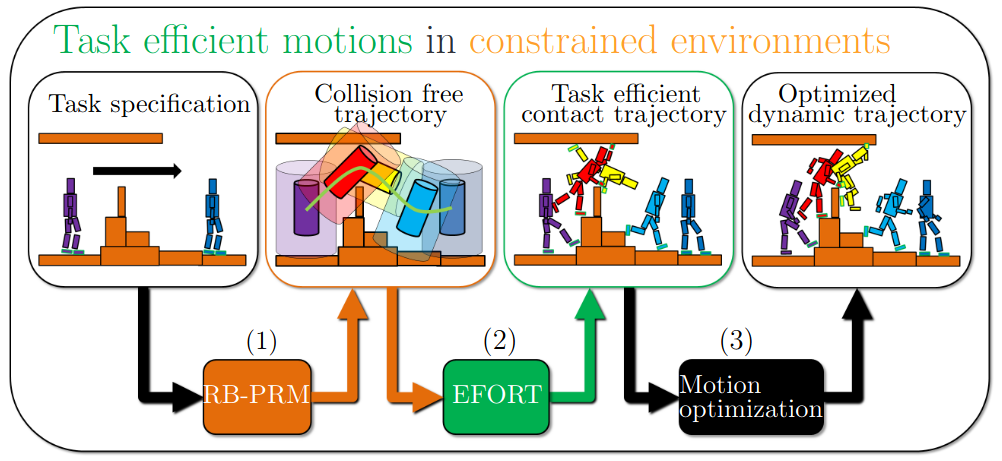
\includegraphics[width=0.8\textwidth]{Figures/Chapter_SOTA//diagram_steve_thesis.png}
    \caption{Motion-before-contact strategy, planning a rough robot trajectory to guide the contact planning. Source: Tonneau \cite{thesis_steve}.}
    \label{fig:cp_mbc}
\end{figure}

Planning only a few steps ahead requires the careful guidance of the robot to avoid falling into local minima.
On the other hand, planning several steps is subject to combinatorics, making the problem exponentially expensive to compute in function of the number of steps and the terrain complexity (e.g. many choices of potential contact surfaces).

Inspired by some previous works on character animation \cite{thesis_kuffner_1999, pettre_2_stages_2003}, the motion-before-contact strategy alleviates these limitations by adding a higher level planning layer, thus further dividing the contact planning problem into two modules:
\begin{enumerate}
    \item A guide path planner, to generate a rough trajectory the robot has to follow to go through the environment (e.g. a robot base collision-free trajectory, see Figure \ref{fig:cp_mbc}).
    \item A contact planner, to compute the contacts along this trajectory.
\end{enumerate}
Previously presented contact planners can thus be adapted to use a guide path to constrain the search for feasible contacts in the environment, and to obtain additional information about the path to traverse.

\begin{figure}[t]
    \centering
    \captionsetup[subfigure]{justification=centering}
    \begin{subfigure}[t]{0.48\linewidth}
    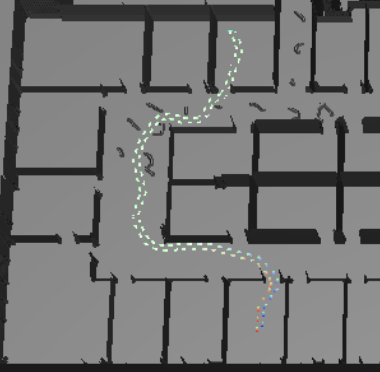
\includegraphics[width=\textwidth,height=4.5cm]{Figures/Chapter_SOTA//chestnutt_2004.png}
    \caption{Chestnutt et al. \cite{chestnutt_tiered_planning_2004}}
    \label{fig:cp_mbc_works_0}
    \end{subfigure}
    \begin{subfigure}[t]{0.48\linewidth}
    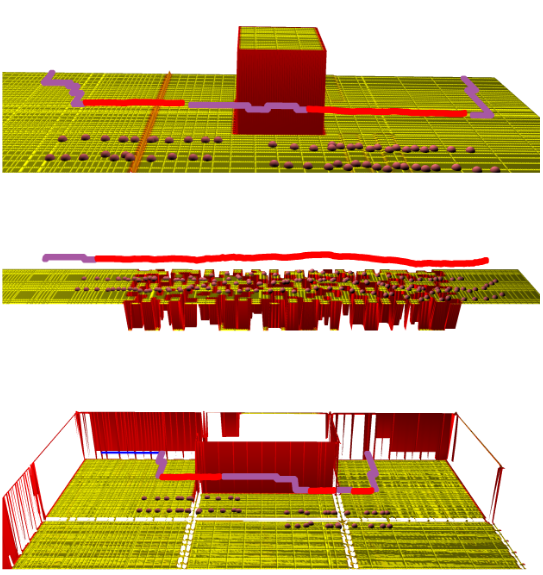
\includegraphics[width=\textwidth,height=4.5cm]{Figures/Chapter_SOTA//brandao_traversability.png}
    \caption{Brandao et al. \cite{brandao_multimode_2019}}
    \label{fig:cp_mbc_works_1}
    \end{subfigure}
    \caption{Examples of work on motion-before-contact planning.}
\end{figure}

\paragraph{Guiding a contact planner.}
Planning a robot trajectory is a problem of lower complexity that can be used for both horizons of contact planning.
Using a guide to control the input direction of short horizon footstep planners, can potentially solve their local minima issue \cite{norby_skd_2022}. 
On long horizon planners, the guide can constrain the search for footsteps around the guide, thus alleviating the combinatorics of the problem \cite{Hildebrandt_lola_2017}.

Using this architecture, Chestnutt et al. first manually define a graph searched for a 2D collision-free path \cite{chestnutt_tiered_planning_2004, Chestnutt2007NavigationPF} (Figure \ref{fig:cp_mbc_works_0}) or interactively drawing it on a user interface \cite{chestnutt_2009_interactive_guide}. This path then guides an A*-based contact planner.
Similarly, Yoshida et al. \cite{yoshida_2005} introduce a guide planner using a bounding box to model the robot moving while manipulating a large object. Their method generates collision-free trajectories to go through the environment, then followed by a pattern generator.

These works have been extended to more complex terrains with a reachability condition to plan 3D guide paths, before computing a sequence of contacts along it \cite{RB-PRM, AcyclicCP, rough_terrain_reachability_hutter_2021}.
% This condition is used in a sampling-based path planning algorithm, 
Using this condition, guide paths can also help in solving the surface selection problem of continuous contact planning methods \cite{sl1m_v2}.
In a model predictive control fashion, Risbourg et al. \cite{fanny_mip_solo} 
use a guide to obtain candidate contact surfaces and allow real-time short horizon footstep planning with a MIP method on the quadruped Solo.

Motion-before-contact approaches have proven successful in efficiently planning contacts for legged character locomotion \cite{egges_2010, bouyarmane_2009, bouyarmane2018}.
However, it also presents some limitations as explained in \cite{escande_2008}, where the guide should be rough enough to be quickly planned while being \qq{constrained enough} to generate feasible contacts along.


\paragraph{Estimating the traversability.}
Planning a path according to an estimation of the difficulty to traverse the terrain can generate guide paths more likely to be feasible by contact planners.
This strategy has been used to move some quadruped robots through difficult rough environments \cite{kolter_2008, terrain_map_mrinal_2011, winkler_2014, winkler_carlos_2015, wermelinger_2016}. 

% Lin 2018/2021 (traversability)
% Brandao et Havoutis 2019/2020 same
Additionally, the guide paths can give information about the sections of the terrain crossed, permitting different walking strategies in function of its difficulty, also known as the multi-modal planning problem.
To move a humanoid robot in cluttered environments, Lin et al. \cite{lin_traversability_2018} plan a torso guide path using an A* searching algorithm on a cost map, and accounting for the difficulty of traversing the environment. 
They then decompose the guide path into segments, selecting for each one the mode of locomotion (known as multi-modal planning). They switch between simple biped walking or multi-contact locomotion using the robot's hand for increased stability in cluttered environments.
In the same line of work, Brandao et al. \cite{brandao_multimode_2019} use a quadruped robot body path to plan the different modes, such as a walking or trotting gait on flat ground, and a contact planning on terrains requiring careful positioning of footsteps.
Their results demonstrate that multi-modal planning locomotion can potentially achieve faster computation speed than pure footstep planning methods.

% Mini-conclusion: Such approximation considerably improve the computation time by lowering the complexity of the problem, where the goal is just to compute contacts along the collision-free guide given in input.
% Previous works were using it just to avoid collision, but the notion of reachability introduced by steve or carlos (?) is promising for the motion-before-contact strategy.
% Some works also uses the guide in different way: follow exactly the guide to compute the contacts, use the guide only to compute the contacts and ditch it after, use it to prune the surfaces, or use it in the notion of traversability to for multi-modes.
\paragraph{Conclusion on motion-before-contact.}

The motion-before-contact strategy is promising toward faster contact planning for legged robot locomotion.
% I WILL TALK ABOUT IT IN THE NEXT SECTION
%Different methods to generate the guide path have emerged using height maps, grids, or graphs solving a \textit{Navigation task}.

A prior guide path can be used in different ways by contact planners. 
Some works use it to accelerate the search for footsteps around the guide path, while others use it to get information about the traversed terrain to also solve the multi-modal planning problem.

However, this approach also comes with a critical limitation due to the decomposition into sub-problems.
Indeed, we have no guarantee that a guide path is feasible by a given contact planner.
Some works use heuristics to approximate the feasibility of the contact planner and to plan guide paths alleviating this limitation.
These methods for guide path planning will be further covered in the next section on legged navigation.
% I WILL TALK ABOUT IT IN THE NEXT SECTION
%However, their approach remains expensive to compute and the development of some general enough and efficient heuristics remains complex.


\subsection{Conclusion}

% In a hierarchical decomposition of locomotion tasks, contact planning is usually done as contact-before-motion. While a step by step planning is possible, this can lead to local minima on more complex terrains and that is why we often want to plan several footsteps ahead to walk. But this brings a combinatorial aspect to the problem that can lead to high computation time >1s.

% COMMENTED
%Contact planning is a classical low complexity approach to solve the locomotion problem. The contact-before-motion strategy has been widely used in robotics to plan feasible footsteps in complex environments. Short horizon planning is fast to compute, but can be prone to local minima. Inversely, long horizon planning allows to ensure the completeness of the problem, at the cost of a higher computation time, where the inherent combinatorics of the problem has to be solved using discrete or continuous methods, and can lead to exponential computation times in function of the size of the problem.

% COMMENTED
%To alleviate these limitations, the motion-before-contact strategy proposes to plan a rough robot path in the environment prior to the contact planning phase. Using a high-level path is promising to guide or constrain the search for footsteps, while getting some information about the terrain to adopt the best walking strategy. The motion-before-contact approach has the potential to alleviate the limitation of current contact planner, that are the combinatorics or the local minima. Thus, it is a promising strategy for interactive replanning. However, using a guide also raises the problem of the non-guaranteed feasibility of the guide path with the contact planners. 

% COMMENTED
%Finally, generating a guide path introduces a new dimension to the locomotion problem that has been widely studied in other fields of the literature: the \textit{navigation} task.

% COMMENT NICOLAS: mieux articuler la conclu
% 1 - contact planning is yet a needed stage when generating complex movements.
% 2 - It relies in general to specific/adhoc model reduction combined to dedicated algorithms to explicitely tackle the discrete nature of contact sequences.
% 3 - We prefer MBC, because CBM leads to untractable complexity.
% 4 - MBC in turns implies guide planning, also separately handled as legged navigation.

Contact planning is yet a needed stage to generate, in tractable time, complex movement on legged robots.

This task relies on specific model reduction, to ensure footsteps feasibility, that is combined with dedicated algorithms to tackle the discrete nature of finding contact sequences.

In this section, we categorized contact planners into two categories.
The \textit{contact-before-motion} approach can lead to local minima on short horizon planning, and become computationally intractable a longer horizon.
That is why our research will focus on \textit{motion-before-contact}, that is promising to alleviate these limitations.
However, it raises the problem of the non-guaranteed feasibility of the guide path with a given contact planner.

The motion-before-contact approach in turn implies guide planning, that is separately handled as a legged navigation task.


%About these walking strategies, an interrogation we would like to raise and that has not been totally answered is: \textit{Is there a real benefits for longer horizon over short horizon contact planning in most scenarios ?}
%In the context of the free-climbing problem \cite{bretl2006}, it is trivial to solve the combinatorics to find the optimal sequence of contacts. 
%However in the context of legged-locomotion, knowing that a feasible guide exist to move through the terrain, recent works on short horizon planner \cite{fanny_mip_solo, hutter_last_work_nmpc} could already lead to impressive results, removing this combinatorial aspect. \textcolor{blue}{False, to change}
%This question deserves further discussion in the future.

% On the other hand motion-before-contact, with the use of rough body path is promising to alleviate or break this combinatorics, constraining the exploration on a smaller region, prior to a contact planner computing the footsteps along it. 
% From guide path generated by the user or other navigation methods, this strategy has given impressive results with high computation time under a second on the vast majority of these works.
% However this additional hierarchical decomposition leads to a problem : It reduces the number of available solutions and thus, increases the risk to not finding a feasible contact sequence along the guide. (See citation bellow)
% In other words, we have no guarantee that the guide path is feasible by the contact planner.

% Chestnutt: "This is more computationally expensive than solving them separately, but ensures that the planner does not commit to a torso path that is unexecutable."
% "building a good approximation of the cost of reaching one torso position from another is extremely difficult compared to reasoning about the connectivity of stances"
% “difficult to efficiently guarantee that a particular torso path can indeed be followed by the robot (...) reasoning about foot contacts, it is much easier to provide guarantees of executability”

% Zucker says about contact-before-motion: "[ours] is capable of walking over a wider range of terrains, because the body path planner [others] at the most abstract level (...) is too conservative relative to the full range of possible footholds"

% Perrin says: “a high level planner might miss existing solutions that would have been found by the lower level planner”. + Discussion of Escande 2008 about it


\section{Navigation Task \label{sota3}}

\begin{figure}[h]
    \centering
    \captionsetup[subfigure]{justification=centering}
    \begin{subfigure}[t]{0.40\linewidth}
    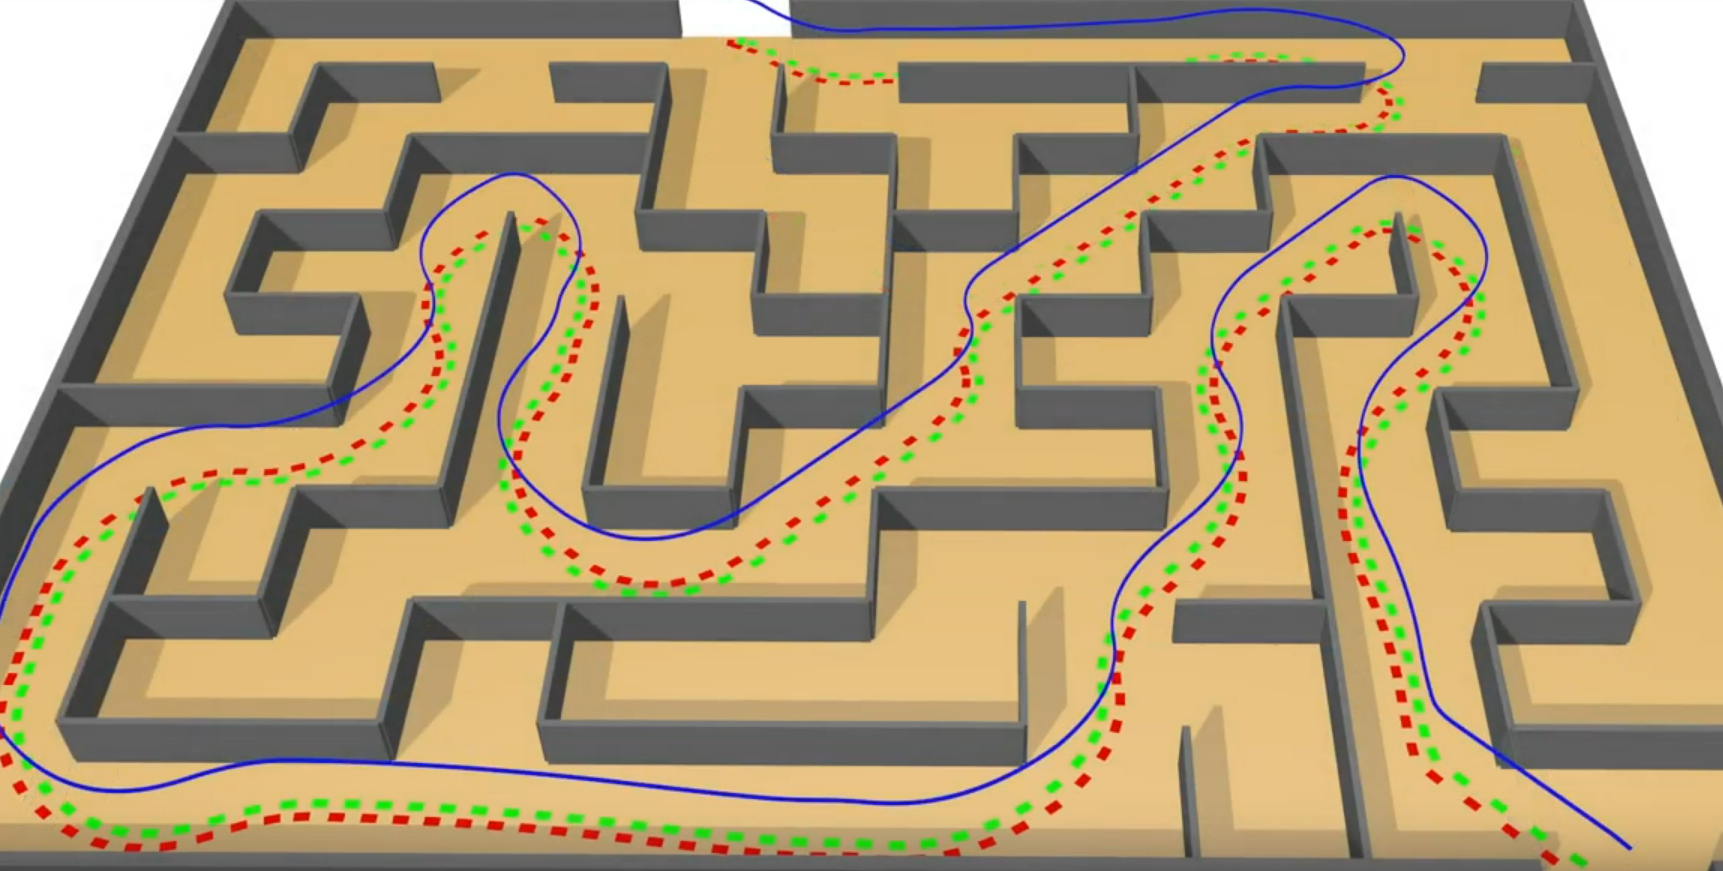
\includegraphics[width=\textwidth,height=4cm]{Figures/Chapter_SOTA//sl1m_maze.png}
    \caption{Global planner}
    \label{fig:nav_ex_0}
    \end{subfigure}
    \begin{subfigure}[t]{0.40\linewidth}
    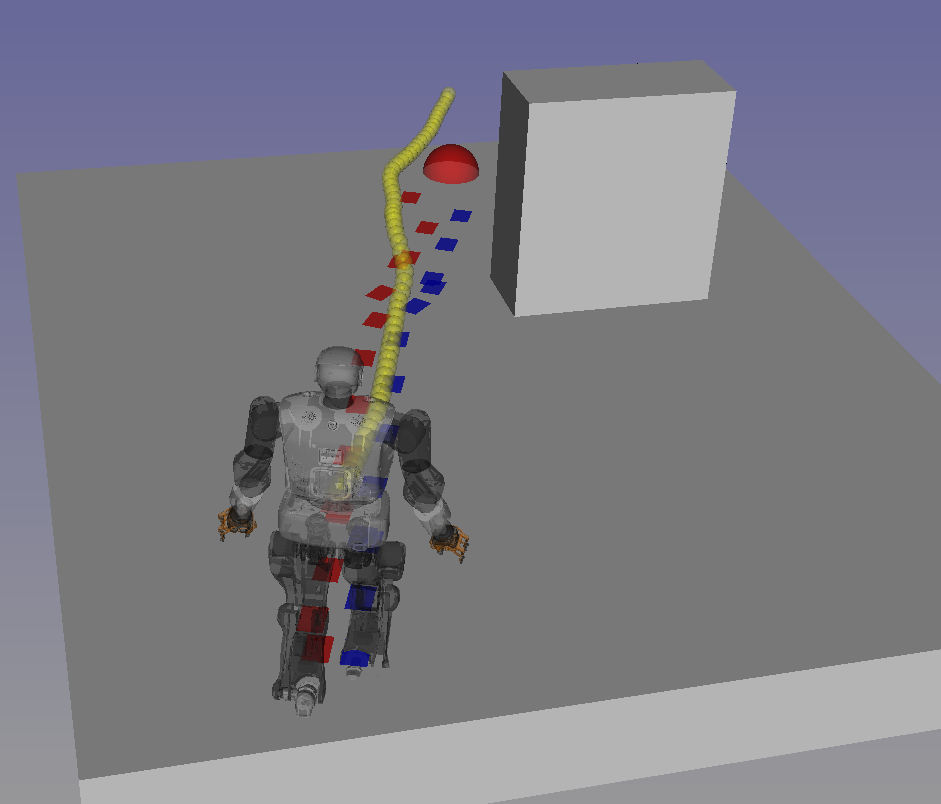
\includegraphics[width=\textwidth,height=4cm,trim={2cm 2cm 2cm 0},clip]{Figures/Chapter_SOTA//local_planning_wall.png}
    \caption{Local planner}
    \label{fig:nav_ex_1}
    \end{subfigure}
    %\label{fig:nav_ex}
    %\begin{subfigure}[t]{0.4\linewidth}
    %includegraphics[width=\textwidth,height=4.5cm]{Figures/Chapter_SOTA//dwa_rl.png}
    %\caption{Patel et al. \cite{patel_dwa_rl_2021}}
    %\label{fig:nav_ex_1}
    %end{subfigure}
    \caption{Navigation task at two different scales. Sources: (a) Tonneau et al. \cite{sl1m_v1}, (b) simulation on HPP \cite{HPP} with Tonneau et al. \cite{sl1m_v1}.}
\end{figure}


Navigation focuses on planning and following a conflict-free path from some initial to goal positions, where conflict-free refers to the satisfaction of validity criteria (e.g. collision-free).

This challenging task has been extensively studied in the context of legged character or other autonomous vehicle navigation.
The environments they move in are often partially known or dynamic, thus requiring fast planning while satisfying optimality criteria.

To solve this problem, the navigation task can be performed with different architectures operating at different scales \cite{review_autonomous_2011}. 
Recent state-of-the-art implementations for crowd simulation \cite{vantoll_microscopic_crowd_2021} or autonomous vehicles, like the ROS navigation stack for 2D navigation \cite{ROS_software}, employ an architecture composed of two modules:
\begin{itemize}
    \item Global planner, that plans a rough feasible path through the environment to a goal (Figure \ref{fig:nav_ex_0}). This is usually performed by \textit{path planning} algorithms that search for sub-goals to reach sequentially with a local planner.
    \item Local planner, that follows the rough path under specified rules. These rules can for example be based on the current sensory information of the robot for collision avoidance (Figure \ref{fig:nav_ex_1}). 
    This is usually performed by \textit{motion planning} (or \textit{trajectory planning}) algorithms that consider the robot or vehicle dynamics.%\textcolor{blue}{This is explained in "The Dynamic Window Approach to Collision Avoidance: of Dieter.}
    In this thesis, we will call such a local planner a \textit{steering method}, which is a widely used term in navigation.
\end{itemize}

Section \ref{subsub:nav:overview} has a pedagogic purpose, in which we will present generic algorithms for both global and local navigation.
Finally, we refer the reader to Section \ref{subsub:nav:legged} for the use of these algorithms in the context of legged robots navigation.

\subsection{Overview: navigation methods\label{subsub:nav:overview}}
We propose to explore the algorithms used in the broad context of navigation.
These algorithms can be categorized depending on the scale they operate in.

\paragraph{Global navigation in known environment.}\mbox{}\\
\begin{figure}[h]
    \centering
    \captionsetup[subfigure]{justification=centering}
    \begin{subfigure}[t]{0.32\linewidth}
    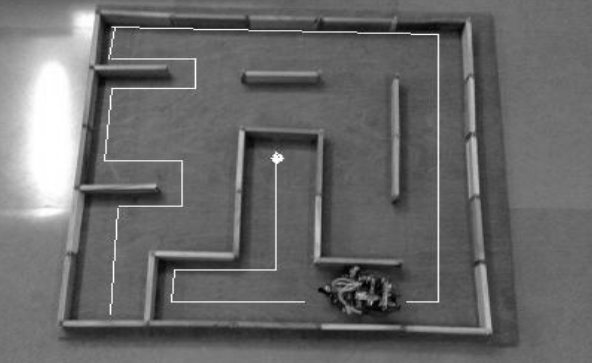
\includegraphics[width=\textwidth,height=3.5cm]{Figures/Chapter_SOTA//micromouse_maze.png}
    \caption{Micromouse challenge}
    \label{fig:global_nav_0}
    \end{subfigure}
    \begin{subfigure}[t]{0.32\linewidth}
    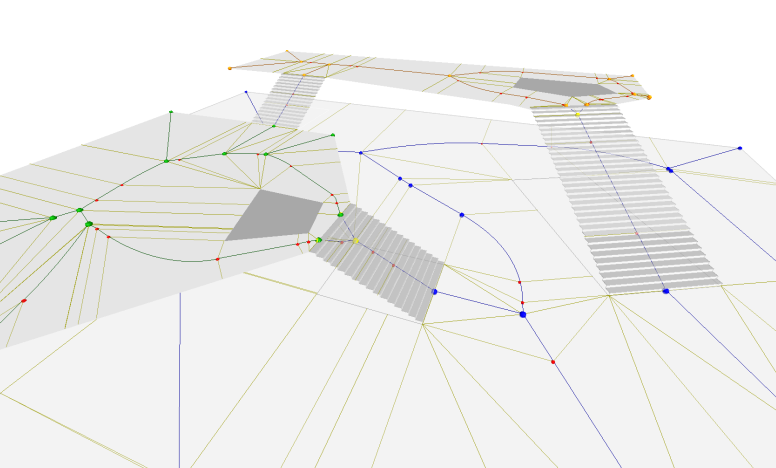
\includegraphics[width=\textwidth,height=3.5cm]{Figures/Chapter_SOTA//navMesh.png}
    \caption{NavMesh}
    \label{fig:global_nav_1}
    \end{subfigure}
    \begin{subfigure}[t]{0.32\linewidth}
    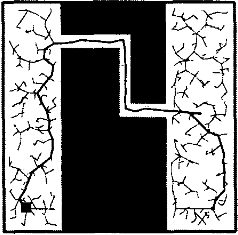
\includegraphics[width=\textwidth,height=3.5cm]{Figures/Chapter_SOTA//rrt_connect.png}
    \caption{RRT-connect}
    \label{fig:global_nav_2}
    \end{subfigure}
    \caption{Examples of global navigation in 2D and 3D, sources: (a) Mishra et al. \cite{micromouse_mishra_2008}, (b) Toll et al. \cite{toll_2011_navMesh} and (c) Palmieri et al. \cite{RRT_distance_palmeieri_2015} \label{fig:global_nav}}
\end{figure}

Consider a complex environment in which the robot has to move from an initial to a goal configuration (Figure \ref{fig:global_nav}).
By knowing the full model of the terrain in 2D or 3D, various strategies have emerged to solve the path planning problem.

We will explore the two main strategies for path planning that are \textit{graph-based} and \textit{sampling-based}.
These methods were previously introduced to solve the discrete contact planning problem (Section \ref{subsub:contact-before-motion}).
%and to solve a navigation task in the context of motion-before-contact strategy. 
Here we will present these path planning algorithms for a wide range of navigation applications.
Due to the global scale they operate on, most path planning algorithms do not consider the kinetics and kinodynamics of the system (e.g. maximum acceleration, velocity and steering angle). 
Indeed it would result in burdensome computation time. 
These constraints are considered by the local motion planners that will be presented in the next Section \ref{subsub:nav:local}.\\

\noindent\textbf{Graph-based searching.}
% Read : Indicative Routes for Path Planning and Crowd Simulation, that explain very well all that.
% Say that from a graph, we have efficient algo to search it, mainly djikstra then A* and all its variations.
A graph is a structure composed of nodes and links, that are the discretized robot base positions and their connections to other nodes respectively.
This graph is then processed by a search algorithm that solves a combinatorial problem to find the shortest path from the initial to the goal configurations. 
These search algorithms have a long history in the path planning field with Depth-First Search, Breadth-First and the well-known Dijkstra algorithm \cite{dijkstra_1959}. 
%These search algorithms have a long history in the path planning field with Depth-First Search, Breadth-First and the well-known Dijkstra algorithm \cite{dijkstra_1959}. 
%The latest uniformly explores the links according to their cost (e.g. path length) and selects the optimal path up to the goal. % (i.e. with the lowest sum of cost)
%A limitation of this uniform exploration strategy is that it can result in high computation time on long paths or in more complex environments.
Numerous search algorithms emerged to more efficiently explore such graphs, among which A* \cite{A_star_1968}, biasing the exploration toward the objective, along with its variants D* \cite{D_star_1994}, for an efficient replanning on unknown or partially known environments, or Anytime Repairing A* (ARA*) \cite{ara_star_2003} finding a suboptimal solution quickly then optimized toward optimality.

Now that we know efficient algorithms exist to search a graph, we are left with the question: \textit{How to build such a graph?}
% Predefined graph "waypoint graphs" => Not much to say here.
Manually specifying each node and link (waypoint graph) is a possibility to ensure the construction of a graph with conflict-free links \cite{waypoints_graph_lars_2002}.%, Chestnutt2003}. 
However, more generic methods requiring less cumbersome manual labor are preferred, such as Voronoi diagrams \cite{voronoi_example_2007} or visibility graphs \cite{visiblity_graph_example_2004}. \\
%\textcolor{blue}{I talk about it, but I do not explain them, it's long enough like that. How to say that I won't explain it here ?}

\noindent\textbf{Grid discretization.}
% Grid => Most the works => % Definition of gried in Philippsen 2005 is ok.
Grids are used to uniformly decompose the environment into cells. 
Each cell corresponds to a node in the graph that is linked to its adjacent neighbors in free space (i.e. not occupied by any obstacle), thus forming a graph covering the full environment on which we use a search algorithm.
% ROS is using 2D grid was well to plan a global path
ROS navigation stack \cite{ROS_software} models the environment as a grid, which is then used for global path planning on mobile robots. The grid can represent an occupancy map indicating the presence of obstacles, or a cost map indicating the difficulty to traverse each cell.
% Path Planning with Modified a Star Algorithm for a Mobile Robot (Duchon 2014)
Several searching algorithms have been introduced for navigation in grid environments, mostly developing variants of A* algorithms to improve the computation time and optimality of the paths \cite{Philippsen_2005, grid_duchon_2014}.
% Micromouse will flood fill
In the Micromouse challenge, where a mouse robot has to explore a maze and then build an optimal path up to the goal (Figure \ref{fig:global_nav_0}), modeling the maze as a grid and planning the shortest path with a flood fill algorithms has been one of the most successful strategy \cite{micromouse_mishra_2008, micromouse_Benavides2018}.
% Integrated path planning and dynamic steering control for autonomous vehicles (Thrope 1986)
%Using a two-level architecture, Krogh et al. \cite{krogh_1986} first compute waypoints on a globally desirable trajectory, then use a local planner to generate conflict-free trajectories in between waypoints.

% Mini conclu on grid
Representing the environment as a grid is a simple yet efficient strategy to compute global 2D paths for various vehicles \cite{car_grid_ferguson_2008, singh_boat_grid_2018, saeed_grid_2020}.
In the same manner, grid decomposition can be extended to 3D using voxels \cite{3d_field_voxel_carsten_2006, uav_aerial_perez_grau_voxel_2017}. However, it raises the dimension of the problem, and so can lead to intractable complexity.\\


\noindent\textbf{Navigation meshes.}
% Navigation meshes
These methods also called NavMesh \cite{navMesh_book_snook_2000} have long been used in the video game industry \cite{Brewer2019TacticalPO} and crowd simulation \cite{van_toll_crowd_sim_2012} to move some characters. 
They use the terrain geometry, grids or voxels to decompose it into convex polygons traversable by a character. From the polygons, we can then generate a graph of conflict-free links (Figure \ref{fig:global_nav_1}).
% Gait mesh + Papers of Geraerts
Toll et al. \cite{toll_2011_navMesh, toll_2018_navMesh_multiLayer} compute navigation meshes in the order of milliseconds using the medial-axis method, then use it to efficiently generate paths for thousands of virtual characters in real-time.
%However, the resulting set of paths can be limited in terms of possibility and require further editing \cite{sketch_navmesh_montana_2019}.
However, it requires a full model of the environment as well as an offline preprocessing phase to build the mesh.
Navigation meshes can be a computationally efficient solution for interactive global navigation, depending on the model of the scene and the NavMesh method used \cite{pettre_comparative_navMesh_2016}.\\


\noindent\textbf{Sampling-based algorithms.\label{subsubpar:sampling_based_algo}}
% Read kris hauser : https://motion.cs.illinois.edu/RoboticSystems/MotionPlanningHigherDimensions.html
Building graphs for navigation in a higher dimension or very large terrains can become intractable, as the combinatorics exponentially increases with the size of the search space \cite{hauser_robotics_systems_draft}.
In these cases, sampling-based strategies such as Probabilistic Road Map (PRM) \cite{prm_1996} and Rapidly-exploring Random Tree (RRT) \cite{RRT_1998} (Figure \ref{fig:global_nav_2}) are particularly efficient to build a graph or a tree respectively.

Sampling-based algorithms have been widely used for navigation, using PRM \cite{move3d_lamiraux_2001, sabo_aerial_fuzzy_2012, mohanta_prm_navigation_2019} and RRT \cite{Zammit2018ComparisonBA} as well as their variants.
The system dynamics can also be considered in the sampling, thus permitting motion planning.
However, it increases the problem dimension, and so the number of samples required and the planning complexity.
As a result, the efficiency of these algorithms boils down to their sampling strategy, and their local planner capabilities to generate link trajectories \cite{kinodynamic_sm_2017, prm_rl_2019}.

%While those algorithms can bias their random sampling to efficiently cover the search space, it is important to note that PRM and RRT both plan a feasible path to the goal and do not consider the optimality of the solution thus often resulting in jerky paths.
%Several variants of these algorithms exist to alleviate their limitations by performing a post-processing phase, but those will not be covered in this state of the art. 
%optimization on the feasible path toward optimality, but those will not be covered in this state of the art.


\noindent\textbf{Conclusion on global navigation task.}
A large panel of algorithms solves the global navigation problem \cite{motion_planning_latombe_1991, planning_algo_lavalle_2006, hauser_robotics_systems_draft}.
As it can be difficult to find which algorithm suits our application, several surveys exist to guide our choice \cite{yang_3D_path_planning_2016, Zammit2018ComparisonBA, patle_nav_mobile_robot_2019}.

Overall, global planners have to demonstrate efficient exploration capabilities of the search space.
Due to the scale they operate in, they often require an expensive offline phase to build the graph or searching time.
As a consequence, those are not suited for replanning in uncertain environments, where the global perception is rarely realistic and unexcepted events can occur.

That is why, it is preferred to combine these global algorithms with a simple linear interpolation to generate collision-free trajectories between graph nodes at a minimal cost, without considering the system dynamics. 
The graph is then searched to get a rough path (i.e. waypoints to reach sequentially), that is then followed by a local planner to handle environment uncertainty.



\paragraph{Local Navigation for environment uncertainty\label{subsub:nav:local}}\mbox{}\\
\begin{figure}[h]
    \centering
    \captionsetup[subfigure]{justification=centering}
    \begin{subfigure}[t]{0.4\linewidth}
    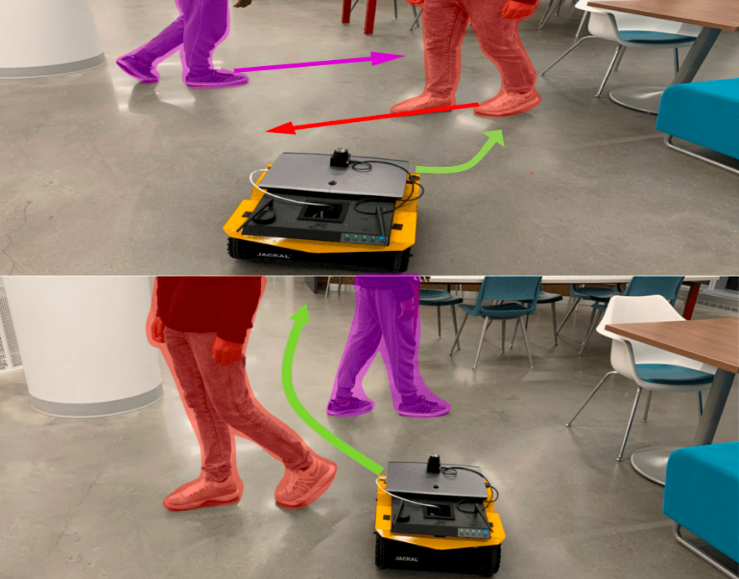
\includegraphics[width=\textwidth,height=4.5cm]{Figures/Chapter_SOTA//dwa_rl.png}
    \caption{Patel et al. \cite{patel_dwa_rl_2021}}
    \label{fig:local_nav_0}
    \end{subfigure}
    \begin{subfigure}[t]{0.5\linewidth}
    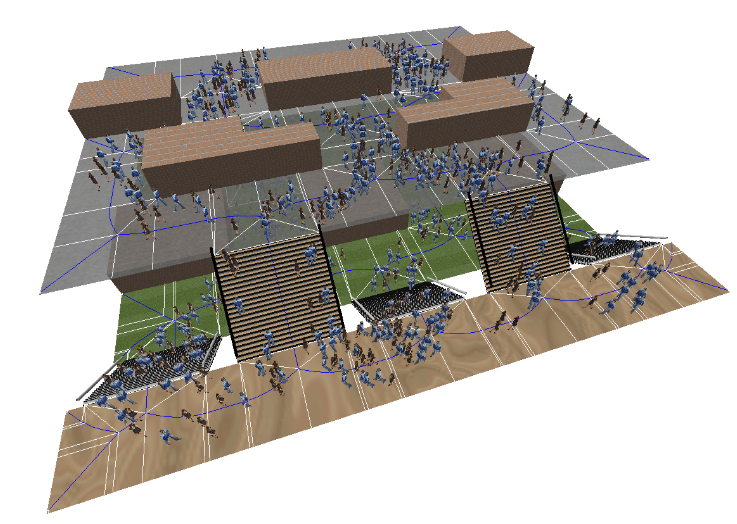
\includegraphics[width=\textwidth,height=4.5cm]{Figures/Chapter_SOTA//real_time_density_geraerts.png}
    \caption{Toll et al. \cite{van_toll_crowd_sim_2012}}
    \label{fig:local_nav_1}
    \end{subfigure}
    \caption{Examples of local navigation: (a) a mobile robot and (b) characters in a crowd simulation locally avoiding collisions with the terrain and other people.}
    \label{fig:local_nav}
\end{figure}

% Discussion about the definition of a steering method:
% From \cite{DIMT}, \qq{A steering method is able to exactly and optimally connect any two states while ignoring obstacles}. 
% From \cite{PRM_RRT_SM}, the function steer returns a point $z$ such that $z$ is closer to $y$ than $x$. If we follow this definition, then this is exactly what LEAS does.
% The steer function is also well expained in RL-RRT \cite{RL_RRT}, Pettre in microscopic crowd.

%\stn{donner l algo et ou une figure ça simplifierait la comprehension}

A local planner computes a trajectory between two points generated by a global planner.
In the context of navigation, we call such a local planner a \textit{steering method} (Figure \ref{fig:local_nav}). 
%It guides the trajectory toward a distant objective or its direction.
These local planners have been extensively used in navigation tasks for fast and local replanning.
Contrary to global planners, steering methods often do not require a guarantee of completeness or optimality but need to produce local paths under desired criteria, such as fast computation, collision-avoidance behavior, or kinetic and kinodynamic constraints.\\


\noindent\textbf{Definition of a steering method.}
The definition of the word \textit{steering} is \qq{the control of a vehicle to make it follow a route or direction}.
However, we identify in previous works different definitions for the term \qq{steering method}.

The first definition states that a steering method \qq{computes an open-loop trajectory that brings a nonholonomic system from an initial state to a goal state without the presence of obstacles} \cite{randomized_kino_planning_lavalle_2001}. 
This definition has been used in other works \cite{DIMT, move3d_lamiraux_2001} specifying that such steering methods exactly connect two states.

A broader definition is a local planner that \qq{follows the rough path while adhering to certain local rules} (e.g. collision-avoidance) \cite{van_toll_crowd_sim_2012}. 
Adherence to these rules can imply some reactive behaviors from observations of the terrain such as the presence of obstacles. % Pas obligatoirement
This definition is used in navigation \cite{ondrej_pettre_steering_vision_2010,prm_rl_2019} where the characters or vehicles are often steered toward waypoints obtained by global path planning algorithms, but may not reach them exactly. 
% https://arxiv.org/pdf/1902.09458.pdf Page 4
%Such definition also matches the \textit{base local planner} controller of the ROS navigation stack \cite{ROS_software} using a non-exact steering method (dynamic window approach \cite{}).

%In the context of character navigation as in this thesis, we use the broader definition that is more relevant.
In this thesis, we will use the broader definition that is more relevant in the context of legged robot navigation.\\
%Indeed, in most scenarios, we do not need the character to reach exactly the sub-goal positions but just a small radius around it.
%Finally, not considering the obstacles during the local planning presents a fast computation time with a purely model-based approach that however needs to rely heavily on conflict checking inside the higher level path planning algorithms, and inversely for a steering method with terrain-aware capabilities.
%For the sake of simplicity, we will employ this definition for both terms \textit{steering method} and \textit{local planner}.% while keeping in mind that we use them in the context of legged character locomotion.

% Focus on the "steering": Most of these works uses path planning that uses a steer function, and most of the time, it's model-based: linear interpolation in SE2 or SE3, or subject to constraints on the acceleration (DIMT=Kino).
% But we can also take some inspiration from "control" methods for navigation.
% Many works working on the steering for autonomous vehicles 2D, where RL-RRT is kinda the same. Then there is all the work on crowd sim that solves a sligthly different problems but use similar controls (mostly in 2D, using rays or velocity fields).
% Terrain-aware: heightmap, voxel map and grid map.
% Notion of traversability (Lin and Hutter) to know if a path is easy to take or not. It's mostly in their work to chose between walking mode, multicontact or safe footstep planning, but it kinda attempt to solve the feasibility problem with the contact planner.

% I will put the potential field here, see the paper corridor map that explains it very well.
% Indicative Routes for Path Planning and Crowd Simulation : "In general, reactive steering is based on variants of potential field methods (...) but stuck in local minima"
% Talk about CMM and ICM yes.

% I will have to talk about the divisions, see the survey of yang 2016
% Difference in computation between maths and other methods ? what's the best ?
% Also how do we define what is an "obstacle" in 3D. In 2D it's simple, but 3D no. See thier prm for "ground robots".


\noindent\textbf{Terrain-free steering methods.}
Computing a trajectory connecting exactly two points without considering the environment can be done efficiently with model-based approaches.

% Interpolation techniques
% Linear interpolation
% Curves
Interpolation methods consist in computing a curve passing exactly through all the given sub-goals \cite{interpolation_methods_bourke_1999}. Linear interpolation is the simplest and fastest way to link two configurations in space, making it the default steering method of most graph-based and sampling-based algorithms, %and has been widely used in the context of legged robot navigation \cite{rough_terrain_reachability_hutter_2021, AcyclicCP}. 

% Trajectory optimizers as DIMT
Other interpolation methods such as bezier, spline, and hermite curves exist to obtain smooth and continuous trajectories.
Those curves can be a solution to perform motion planning, which regroups different terms as kinodynamic \cite{randomized_kino_planning_lavalle_2001, DIMT} or nonholonomic planning, that must account for constraints on the system dynamics (i.e. velocity and acceleration ) or whose state depends on the path taken respectively.
%Kinodynamic steering methods have seen some success combined with PRM \cite{florent_motion_planning_car_2001} or 
%RRT global planners . 
%One of these kinodynamic planners is the double-integrator minimum time, that has been used for planning on robot manipulators \cite{DIMT}. 
%This method has also been used to plan guide paths in the context of the navigation of humanoid robots \cite{kinodynamic_sm_2017} which will be used for comparisons throughout this thesis.

These steering methods exactly connect two sub-goals and are fast to compute as they ignore obstacles.
However, they heavily rely on conflict checking by the global planner when applied to complex environments. 
This can often be burdensome in algorithms such as PRM and limit their use in applications with environmental uncertainty which requires fast local replanning.\\


\noindent\textbf{Terrain-aware model-based steering methods.}
Computing a conflict-free trajectory considering the environment is another steering strategy. 
Those additional conflict-free constraints permit a local replanning in function of the environment observations, at a higher computation cost compared to terrain-free steering methods.

% STOMP => Consider obstacles, but stochastic and derivative-free
Local planning can be posed as an optimal control problem \cite{optimal_control_path_planning}. 
Liu et al. \cite{liu_mpc_path_planning_2017} use a model predictive control to enforce collision avoidance with other vehicles in the context of autonomous driving.
Depending on the formulation of the problem and the constraints modeling the environment, these optimization methods can be an efficient solution for locally terrain-aware planning.

% Potential field => Used in Corridor map and Explicit Corridor
Potential field \cite{potential_field_1992} is a common technique for path planning using local information about the environment \cite{mpc_potential_field_car_2017}. 
This method sees the terrain as an energy potential landscape where obstacles will repulse the robot, while the goal attracts it.
While this method could be used for global planning, it is by nature prone to local minima and therefore more suited for local and reactive terrain-aware planning.
Potential field has seen some success in crowd simulation with the corridor map method \cite{corridor_geraerts_2007, explicit_corridors_2010}, computing first a global path to follow, then locally planning some collision-free paths according to a potential field.

Some of the most widely used local motion planner for collision-avoidance in vehicle navigation are the Dynamic-Window Approach (DWA) \cite{dynamic_window_fox_1997} and the Time-elastic-band \cite{elastic_band_2013}, both presenting their advantages \cite{dwa_vs_teb_2021_rosmann, dimitri_these_2021}, and implemented in the ROS navigation stack \cite{ROS_software}.
% DWA (dieter 1997) => Does consider the terrain and collisions etc.
Dynamic-Window Approach (DWA) \cite{dynamic_window_fox_1997} discretizes the control space of the robot to generate a set of candidate trajectories. 
The best trajectory is then selected based on a user-defined score (e.g. collision avoidance, clearance to obstacles, distance to goal). Those steps are performed continuously during the navigation and permit a fast replanning. However, this method can be computationally burdensome depending on the discretization of the control space, and the complexity of the conflict checking along the candidate trajectories.
% TEB
Time-elastic-band \cite{elastic_band_2013} optimizes a robot trajectory generated by a global planner. This trajectory can be seen as an elastic band that will be modified considering some objectives such as minimizing its path length or time, or obstacle avoidance.

% Velocity field => crowd sim multi char
% ORCA
The crowd simulation field has also developed methods for local collision-avoidance behaviors between autonomous agents and their environment. One of them is the Optimal Reciprocal Collision Avoidance (ORCA) algorithm \cite{orca_2011} selecting the best action to compute collision-free motions for thousands of characters in real time (Figure \ref{fig:local_nav_1}). 
These methods solve a particular problem that is the collision-avoidance in highly dynamic environments, subject to different criteria (e.g. social distances or group behaviors). Those are not applied in the context of this thesis, but we refer the reader to the survey of Toll et al. \cite{vantoll_microscopic_crowd_2021} for further details.\\


\noindent\textbf{Terrain-aware RL steering methods.}
% MDP for discrete actions, possible on grid etc also. (see the book of hauser)
Reinforcement learning has seen a lot of success in locally terrain-aware navigation due to its perception and generalization capabilities, and robustness to uncertainty.

% Crowd simulation
Controlling an agent in velocity and orientation, RL controllers have been used for steering in crowd simulation \cite{survey_rl_animation_pettre_2022} and autonomous robot navigation \cite{collision_avoidance_rl_multiagent_chen_2016, survey_rl_driving_kiran_2020} in uncertain and dynamic environments.
Lee et al. \cite{jaedong_2018_crowd_rl} present a method to teach an agent collision avoidance behavior, using rays to detect obstacles and other agents.
Francis et al. \cite{prm_rl_2019} learn an RL steering control over linear and angular velocity on an autonomous mobile robot for local navigation. They also use this steering method inside a PRM to evaluate the links feasibility and build a graph.
%Multi-Agent RL (MARL) is an interesting approach to learn interactions between two characters. 
%Chen et al. \cite{collision_avoidance_rl_multiagent_chen_2016} present a decentralized multi-agent approach to learn collision avoidance by reinforcement on two mobile robots. Their results show that the learned policy can generate natural and smooth trajectories while avoiding other humans or virtual agents.
Combining RL with model-based approaches Patel et al. \cite{patel_dwa_rl_2021} generate trajectory candidates using the Dynamic Window Approach (DWA), then learn a policy to select the best candidate (Figure \ref{fig:local_nav_0}).
Finally, Muller et al. \cite{dwa_gan} use an evolutionary algorithm to generate candidate trajectories, thus potentially generating better motion plans than a classical DWA approach.

Different representations of the environment can be used to learn local planners such as velocity fields \cite{deep_multiagent_crowd_2020}, depth images \cite{learn_to_steer_rl_2018}, lidar sensors information \cite{prm_rl_2019, RL_RRT} or occupancy grids \cite{rl_navigation_video_game_2020}.

Reinforcement learning is a powerful tool to achieve behaviors that are complex to engineer with model-based approaches.
In the context of local navigation, those methods tend to adapt well to uncertain or partially known environments.
They are a pertinent choice over model-based approaches to learn how to solve complex navigation tasks while respecting some desired criteria.\\
% We do not talk about evolutionary algorithms in this section that can be a suitable alternative to RL for navigation.
% Paper of deepmind: evolutionary vs rl + majid 2021
% Evolutionary-Group-Based Particle-Swarm-Optimized Fuzzy Controller With Application to Mobile-Robot Navigation in Unknown Environments


\noindent\textbf{Conclusion on local navigation.}
% Discussion on terrain-aware vs terrain-free
%We have seen two definitions of steering methods to locally compute a trajectory between two points. 
Terrain-free steering methods are fast to compute, but have to rely on expensive to compute global planners for conflict checking and replanning when facing environmental uncertainty.

Terrain-aware methods can remove the need for replanning on simple scenarios by generating conflict-free paths. %, however resulting in higher computation times.
%They have been widely used to follow paths computed by global planners.
While model-based approaches can efficiently compute trajectories with collision-avoidance behaviors (e.g. ORCA, DWA), reinforcement learning is particularly promising to learn complex navigation tasks.
It is used in the context of autonomous mobile robot navigation to learn policies collision avoidance with humans, or crowd simulation to learn social distancing and adapting to other agents steering behavior. 
Furthermore, they can generalize well to unexpected events and partially known environments by using rich perceptual observations.




\subsection{Navigation task for legged robot locomotion\label{subsub:nav:legged}}
\begin{figure}[h]
    \centering
    \captionsetup[subfigure]{justification=centering}
    \begin{subfigure}[t]{0.40\linewidth}
    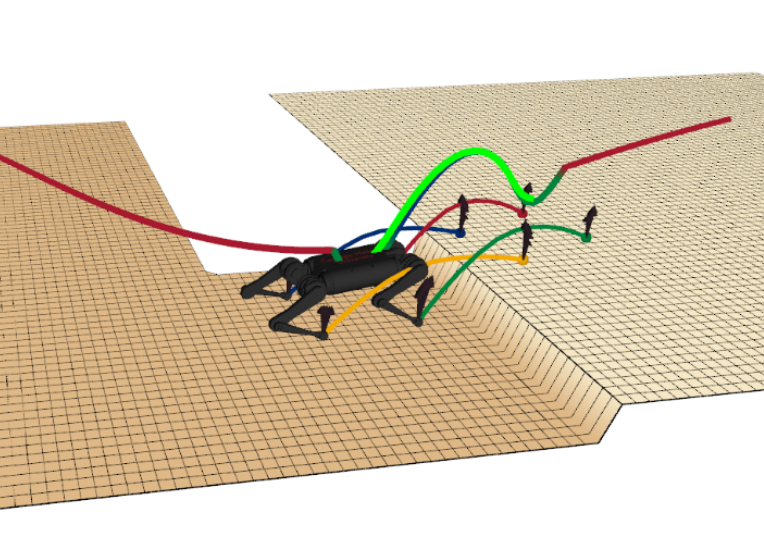
\includegraphics[width=\textwidth,height=4.5cm]{Figures/Chapter_SOTA//norby_2022.png}
    \caption{Norby et al. \cite{norby_skd_2022}}
    \label{fig:legged_nav_0}
    \end{subfigure}
    \begin{subfigure}[t]{0.40\linewidth}
    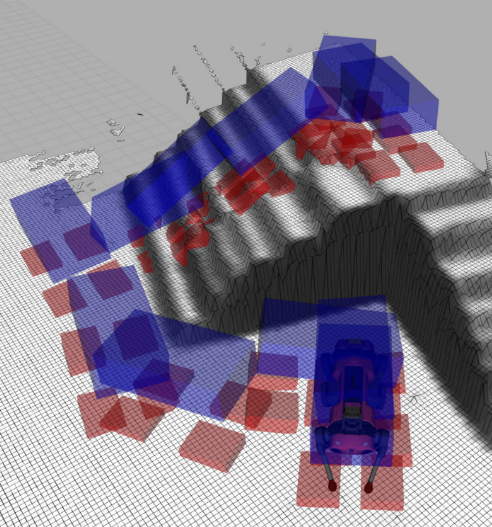
\includegraphics[width=\textwidth,height=4.5cm]{Figures/Chapter_SOTA//hutter_guide_path.png}
    \caption{Wellhausen et al. \cite{rough_terrain_reachability_hutter_2021}}
    \label{fig:legged_nav_1}
    \end{subfigure}
    \caption{Legged robot navigation for motion-before-contact planning.}
\end{figure}

We now want to focus on the application of navigation algorithms for legged robot locomotion.

% Chestnutt 2003 => waypoint graph
In the context of motion-before-contact, manually defining the guide path to follow is a solution for fixed scenarios \cite{Chestnutt2003}.
However, automatizing their generation with a navigation algorithm is required to cover a larger panel of terrains \cite{darpa_hutter_2022}.
%Two main approaches have emerged to for guide planning prior to a contact planner.

The problem these planners have to solve is: \textit{How to generate a feasible guide path for the contact planner?}
%We succintly answered this question in Section \ref{subsub:motion_before_contact} by explaining how the guide can be used by contact planners.
%In this section, we will go more in-depth into the algorithms employed to achieve such a task.

% Most contact-before-motion approaches have been seen in the previous section.
% Here, we will just see what they used to generate the guide paths.
% But it's very limited, not a lot of work on it.


% === Conclusion on feasiblity of the guide by the CP ===
% Waypoint graph => they consider that it's good enough
% Grid => They consider that the heuristics score used to compute the guide is enough.
% Acyclic + hutter => They consider that the reachability condition is sufficient.
% Brandao => They trust their local planner (A*)

\paragraph{Collision-avoidance.}
% Classical global planning algorithms
% Hildebrandt => Elastic band
Avoiding collisions between the robot body and the terrain is a necessary condition for contact planning.

All navigation algorithms previously presented solve this problem, and could thus be used for legged character navigation.
Hildebrandt et al. \cite{Hildebrandt_lola_2017} generate a collision-free guide path using a Time-elastic-band as a steering method. The guide path is then used to guide the search of their A*-based contact planner.

While collision avoidance is necessary, it is often not sufficient to ensure the guide feasibility of a given contact planner on complex terrains.

\paragraph{Cost map for terrain traversability.}
To locomote quadruped robots on rough terrains during the DARPA challenge, heuristics have been used to evaluate the likelihood for a body position to find feasible contacts \cite{kolter_2008, terrain_map_mrinal_2011}.

% Grid => kolter / winkler / Arain 2013 / Wermelinger 2016
Works with the same approach \cite{winkler_2014, wermelinger_2016} discretizes the terrain into a body cost map (grid), then used to plan a guide path. As a result, such paths are more likely to be feasible by a contact planner.
But these approaches rely on manually designed heuristics, that could poorly approximate a given contact planner capabilities.
Lin et al. \cite{lin_traversability_2018} alleviate this limitation by learning a regressor to estimate terrain traversability. They learn one estimator for each of their contact planning strategy in multiple environments, then use it to build a 2D cost map.

However, planning guide paths with a high traversability score is not yet sufficient to ensure contact planning success.
Moreover, it relies on computationally expensive offline and online phases, to build the cost map and search it respectively. 
As a consequence, such a strategy is not yet tractable for real-time applications.

% Humanoid => Lin, he uses a cost-based grid as well. Explain specifically.
% It may not be useful to cite it here.

\paragraph{Robot kinematic reachability.}
% Linear + PRM => Hutter + Acyclic
% Kinodynamic + RRT => Pierre + Norby 2020/2022
% NavMesh => brandao
The reachability condition introduced by Tonneau et al. \cite{RB-PRM} has proven successful to generate guide paths on complex terrains prior to contact planning.
They use an approximation of the robot range of motion, and ensure that the robot can reach the terrain all along the path.

An approach is to incorporate these conditions in sampling-based path planning algorithms \cite{sl1m_v2, fanny_mip_solo}.
Some works use a PRM with a linear interpolation method \cite{AcyclicCP} for navigation and contact planning in tractable computation time, or RRT with model-based kinodynamic steering methods \cite{kinodynamic_sm_2017} for dynamic locomotion.
In this line of work, Norby et al. \cite{norby_skd_2022} use a kinodynamic body path planner to guide their short-horizon contact planner. Their result shows a quadruped robot walking and jumping to cross through uneven terrains (Figure \ref{fig:legged_nav_0}).

Combining reachability condition and foothold estimator, Wellhausen et al. \cite{rough_terrain_reachability_hutter_2021} learn a foothold score predictor in a supervised fashion. This predictor is then used to remove geometry from the reachability space.
Finally, they employ the reachability condition with a PRM and linear interpolation to plan guide paths in complex terrains (Figure \ref{fig:legged_nav_1}).
By doing so, they ensure that robot configurations along the guide can reach more suitable surfaces to step on, and so improve the contact planning success rate.

% What is the problem => On a plus la notion de traversabilité. Le terrain peut être atteignable oui, mais pas sûr qu'on puisse trouver une sequence de contact dessus.
Previous works consider the reachability condition as being sufficient to approximate the feasibility of their contact planner. However, this condition may not be sufficient to generalize to the large panel of contact planning strategies.
Moreover, this condition requires particular fine-tuning.
Overestimating the robot range of motion can lead to unfeasible guide paths.
Inversely, considering only a small range of motion can increase the guide success with a given contact planner, but also limit the guide planning navigation possibilities.

%Guide paths generated have also been used to help solving the surface selection problem of continuous contact planning methods \cite{sl1m_v2} (Figure \ref{fig:cp_mbc_1}).
%In a model predictive control fashion, Risbourg et al. \cite{fanny_mip_solo}  use a guide to obtain candidate contact surfaces and allow a real-time for short horizon footstep planning with a MIP method on the quadruped Solo.


\paragraph{Conclusion on legged robot navigation.}
% Norby: The global planner is critical to this pipeline due to its place at the top of the planning stack. A good global planner must have an accurate idea of what the robot can and cannot do to ensure that the other layers can resolve the motion, but also must have a long enough horizon to avoid local minima which is difficult to achieve in real time. 
In motion-before-contact, guide planning is critical due to its place at the top of the planning stack as stated by Norby et al. \cite{norby_skd_2022}.
Such guide paths must take into account the robot capabilities, and ensure the success of the contact planning.

A panel of strategies emerged to increase the success rate (or compatibility) of the guide with contact planners.
However, they either rely on often necessary but not sufficient conditions (e.g. collision-avoidance, reachability) or on heuristics to improve the likelihood of success that are computationally untractable.


\subsection{Conclusion}

% Talk about all navigation stuff and what exist => It's a jungle.
Navigation at both global and local scales has been extensively studied for a wide variety of applications, ranging from autonomous vehicle navigation to crowd simulation.
% Talk about what is actually done in legged robots relatively to that
In the context of legged robot locomotion and more specifically motion-before-contact approaches, these algorithms can be used to plan guide paths prior to contact planning.

% Very little works on guide feasibility. They conditions, then consider that it's ok.
% cost map for traversability is nice to improve the success rate but not tractable yet.
Legged navigation methods have to solve the critical problem that is the feasibility of the guide path by a given contact planner.
In spite of a few successes with heuristics, no work has yet fully addressed this problem in a tractable computation time.

%Most of previous works consider that collision-avoidance and reachability conditions along the guide.
%However, they are often not sufficient to ensure contact planning success.
%In the search for a general solution 
%Reinforcement learning has demonstrated impressive navigation 

% ================================================================


% However following the resulting rough global path with a terrain-aware steering method is better to consider the dynamic of the system and locally consider replanning for uncertainties in the environment. (corridor map do that for ex, or nav mesh)

% We did not explore all local and global planning strategies and focused on the one that could potentially be applied in this thesis for a character navigation task. More information can be found in the draft of Kris Hauser \cite{hauser_robotics_systems_draft} as well as the reference book in the topic \cite{Robot Motion Planning, planning_algo_lavalle_2006, }

\section{General Conclusion \label{sota4}}
% - General conclusion
%A division of the legged character locomotion problem is still required to interactively plan safe walking motions on complex terrains.
\subsection{Conclusion on legged locomotion strategies.}
We have shown that, despite some recent promising approaches for legged character locomotion, agnostically considering the contact with the terrain to produce whole-body movement is yet unfeasible on real human-sized legged robots.
We believe planning contacts and motion simultaneously to be the most promising solution to achieve this task in the future. However, this approach is yet computationally untractable.

Dividing whole-body control and contact planning is still required to plan safe robot locomotion in real time on complex terrains.
We explored the contact planning problem to automatically generate the contacts to be performed by the whole-body controllers.
We have seen contact planning at two different scales.
Short-horizon planning is fast to compute, but prone to local minima.
% Long horizon planning can offer some guarantee of completeness and optimality to some extent at the cost of a higher computation time.
Long-horizon planning can offer some guarantee of completeness and potential optimality at the cost of a higher computation time.

% Motion-before-contact is promising to alleviate the limitation of both strategies.
% Explain the pipeline.
\textbf{Motion-before-contact} strategy is a promising solution to alleviate the limitations at both planning scales. 
This hierarchical approach contains the following modules:
\begin{enumerate}
    \item A \textbf{guide path planner} generates a rough path the robot has to follow.
    \item A \textbf{contact planner} computes the contacts along this path.
    \item A \textbf{whole-body controller} computes the whole-body motion from these contacts.
\end{enumerate}
% However there is one limitation, that is the non-guarantee of feasibility between the guide and the contact planner. 
% The notion of traversability introduced by lin and brandao kinda goes in this direction, but they solve a multi-modal problem.
% Some heuristics have been developped such as the reachability condition (acyclic) that are necessary but not sufficient.
% We have to see if we have some solutions coming from the other works in navigation.
This hierarchical division of the locomotion problem is a solution for real-time locomotion planning.
However, it also raises the critical problem of the feasibility between the different modules.

The feasibility of the contact plan by the whole-body controller has been solved to some extent in the past years with the study of the centroidal dynamics \cite{prete_static_equilibrium_2016, CROC}.
However, generating feasible guide paths for a given contact planner remains yet a difficult problem. %Previous works focus on the use of heuristics to approximate the contact planner capabilities, that can be either insufficient or too costly to compute \cite{AcyclicCP, winkler_2014}.


% Formulation de la these en exploitant en exploitant les idees de la SOTA centrales.
\subsection{Thesis formulation.}
% "It goes beyond merely summarizing or describing to stake out an interpretation or position that’s not obvious, and others could challenge for good reasons. It’s also arguable in the literal sense that it can be argued, or supported through a thoughtful analysis of your sources. If your argument lacks evidence, readers will think your thesis statement is an opinion or belief as opposed to an argument."

% TOPIC: L'integration d'une tache de navigation dans le contexte du contact planning.
The topic of this thesis is the integration of a \textbf{navigation} task for the legged robot locomotion problem.
Particularly, we want to fix the critical limitation that is the \textbf{feasibility} of navigation paths by the next task the hierarchy, the \textbf{contact planning}.
We formulate our problem as follows: \textit{Can we plan paths more likely feasible by a contact planner?}

% CLAIM: We can see that it helps in accelerating the solving of the contact planning problem, but it raises a critical limitation that is the feasibility of the guide by the contact planner.
Previous works approach the problem with by approximating the contact planner capabilities, such as the \textbf{reachability} condition \cite{RB-PRM} or other manually design heuristics.
Then, they plan paths considering these approximations.
Arguably, they can often be insufficient or too complex to engineer depending on the contact planning strategy \cite{AcyclicCP, winkler_2014}.
%do not necessarily implies that a contact sequence can be planned.
%In general, manually designing efficient heuristics has proven too complex or costly.
%Thereon, we believe that the path feasibility should be learned by collecting \textbf{data} directly from the contact planner.
%Theron, we believe that the generation of feasible paths should be learned by collecting \textbf{data} from results of paths with the contact planner.
Thereon, we believe we should learn how to generate feasible paths by collecting data directly from the contact planner results.

%From path and contact planning data, we should be able to learn how to generate more likely feasible paths.
We choose \textbf{reinforcement learning} to learn such navigation task.
This choice is motivated by the fact that we have no method to generate sufficiently diverse paths to learn from. Therefore, we deemed supervised learning not suitable for this task.

Our work find some inspiration in some recent works on reinforcement learning navigation \cite{prm_rl_2019, jaedong_2018_crowd_rl}. 
This thesis further explores this approach in the context of legged character locomotion.
We answer the question: \textit{How to learn by reinforcement a navigation task with better contact planning feasibility?}

%Our work find some inspiration in recent works on Reinforcement learning for autonomous vehicle navigation \cite{prm_rl_2019} and crowd simulation \cite{jaedong_2018_crowd_rl}.
%In these works, RL agents can navigate using partial observations of the terrain and under complex constraints, that are often too difficult to handle with model-based approaches.
%We investigate this approach in the context of motion-before-contact, where reinforcement learning could be a computationally efficient solution to the guide path feasibility problem.


\chapter{Guide path: LEAS}
\label{sec:LEAS}
\minitoc
\bigskip

%\textcolor{blue}{A REVOIR MAINTENANT COMME ON A ECRIT LA SOTA + INTRO}
In this chapter, we present our method to Learn To Steer a locomotion contact planner \qq{LEAS}, the core module of this thesis. 
Our steering method answers the question: \textit{How to locally navigate complex and unknown terrains subject to validity and collision constraints?}
% Input / Output
LEAS takes as input a desired direction and a local height map of its surrounding terrain, to generate a robot root trajectory.
As many solutions exist to solve such a task, we provide an insight into our design choices and particularly why we use Reinforcement Learning.

Here, we focus on the implementation of LEAS, which will be reused and adapted for different contact planners through Chapters \ref{sec:CP-SB} and \ref{sec:CP-SL1M}.

This chapter is organized as follows: 
In Section \ref{subsec:leas-motivation} we describe the context and the challenges we want to solve. In Section \ref{subsec:leas-RL} we present the specification of the problem and our solution LEAS \cite{LEAS}. We describe it as an RL agent and explain our design choices for its observation, control, and reward to achieve the desired navigation behavior.
In section \ref{subsec:leas-implementation}, we present our implementation regarding the feasibility approximations, the random terrain generation, and the learning architecture.
%additional libraries implemented to optimize the computation time and to create random terrains where to train and evaluate our steering method.
In Section \ref{subsec:leas-results}, we evaluate how LEAS can navigate unknown terrains under reachability and collision avoidance constraints, and compare its results to some other model-based steering methods.
Finally, we discuss the advantages, limitations, and potential improvements of our local navigation method.

\section{Motivation\label{subsec:leas-motivation}}
\subsection{Context\label{subsubsec:context}}

\begin{figure}[h!]
    \centering
    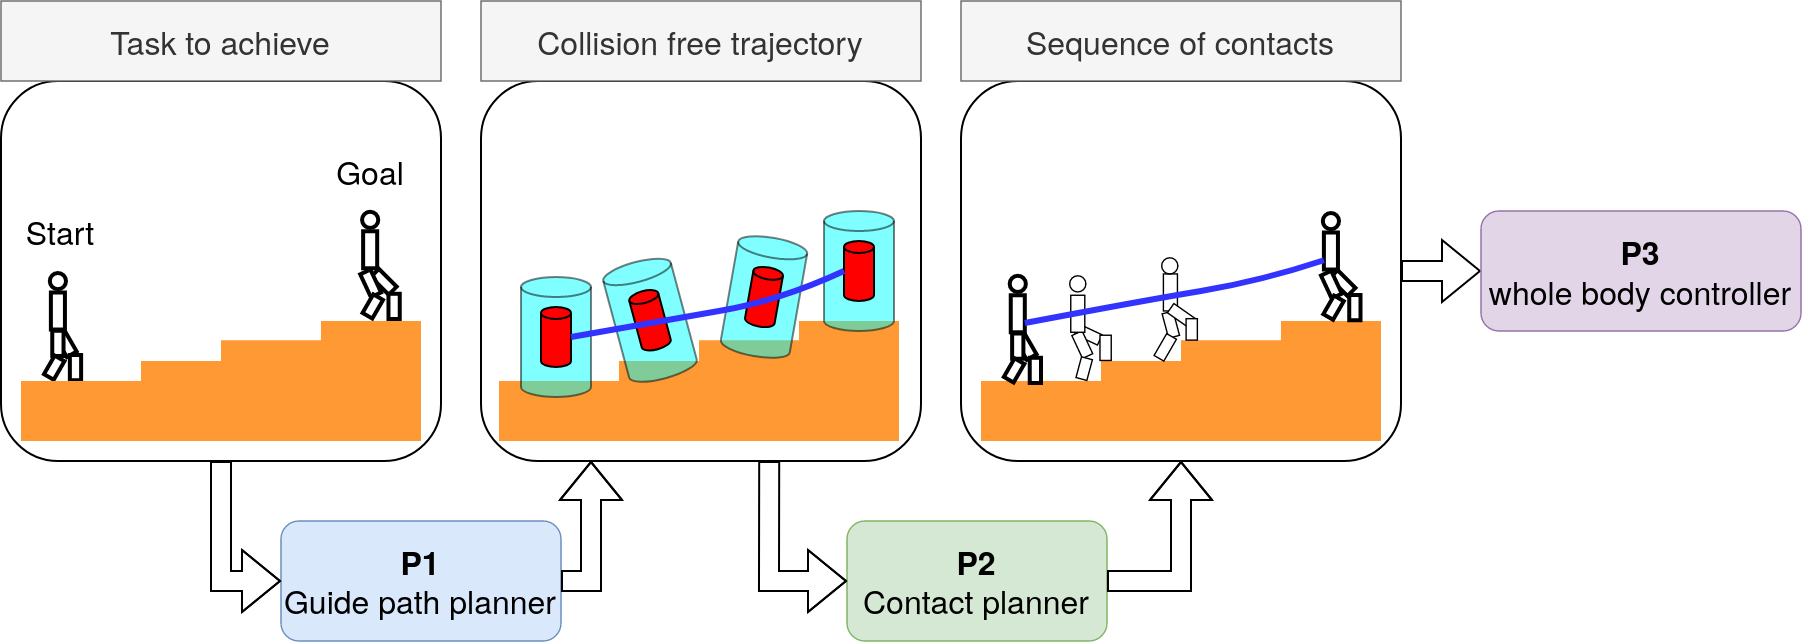
\includegraphics[width=\textwidth]{Figures/Chapter_LEAS/pipeline.png}
    \caption{Pipeline of the Loco3D project addressing the locomotion with a multi-stage approach.}
    \label{fig:pipeline}
\end{figure}


% Re-explain all the context with the division of the locomotion into three phases: Guide path planning - Contact planning - Whole body locomotion.
%In this work, we place ourself in a multi-stage framework \cite{loco3d} that divides the locomotion problem into three sub-tasks as shown on Figure \ref{fig:pipeline}: first \stn{c est quoi p1 ? definis. tu devrais dire que chaque p est un probleme} $P1$ generates a root trajectory, also referred as \qq{guide path}, then $P2$ generates a sequence of contacts on this guide, and finally $P3$ performs these contacts with a whole body controller on the robot.
As discussed in the previous chapter, most of the recent locomotion planners are commonly structured in several hierarchical stages. 
Let us now present in detail how we structured our planner, based on the seminal work that drives the locomotion methodology in our team \cite{loco3d}.
The general organization is shown in Figure \ref{fig:pipeline}.

% All pipeline
The first stage generates a \textit{guide path} ($P1$), i.e. a desired trajectory of the main robot body, referred to as the \textit{root} (i.e. the basis of the torso for Talos). In the second stage, a contact planner ($P2$) computes the contacts along the guide path. In the last stage, a whole-body controller ($P3$) computes the control sent to the robot to perform these contacts.

% What we opt for: motion-before-contact
The decoupling of $P1$ and $P2$ has proven successful in \cite{Escande2008Guide, bouyarmane2009} and later on in \cite{loco3d, RB-PRM}, where each sub-task can be solved independently from each other, thus reducing the complexity of the problem and allowing us to experiment and compare different module implementations. 
%\stn{il manque le papier de bretl, relis bien mon eta tde l art de these pour avoir lhistorique}
%\textcolor{blue}{answer: Bretl and Hauser are contact-before-motion, they will be already cited in the SOTA.}

% Guide path definition
The first module $P1$ generates a guide path, defined in this thesis as a discrete sequence of configurations for the robot root in $SE(3)$ (i.e. position and orientation).
% Division strategy of path planning
This navigation module can be further divided into two parts: a Steering Method (SM) and a path planning algorithm.
The SM locally navigates the terrain following a given direction, while the path planning uses the SM to sequentially reach sub-goals (also called waypoints) up to a distant objective. 
On the resulting guide path, all configurations must respect two constraints as expressed in \cite{RB-PRM} and shown in figure \ref{fig:ROMs}.
%\stn{ça va bien trop vite àa. C est un point important et differentiant. tu dois expliquer comment on fait du sampling based serieusement ici}
%\textcolor{blue}{answer: Sampling-based for path planning you mean? Already done in the SOTA in the path planning section (but briefly). A REVOIR APRES L'ECRITURE DE LA SOTA.}

\begin{figure}
    \centering
    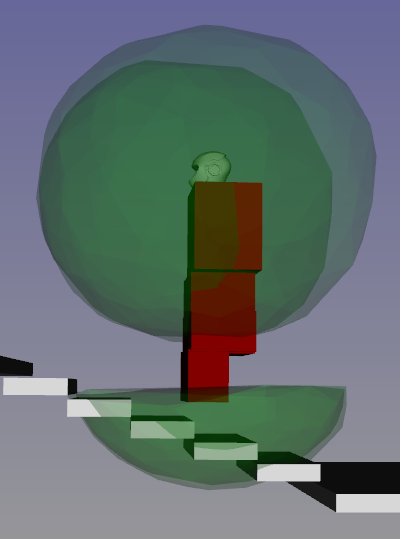
\includegraphics[width=0.3\textwidth]{Figures/Chapter_LEAS/ROMs.png}
    \caption{Validity constraints of the Talos Robot, (green) ranges of motion of each end effector, and (red) the robot trunk. The configuration above is valid as the robot can potentially reach the ground ($\mathcal{R}$) and the trunk is not in collision with the terrain ($\mathcal{C}$).}
    \label{fig:ROMs}
\end{figure}

The first constraint $\mathcal{R}$ is referred to as the \textit{reachability} and imposes that the robot, for a given root configuration, has a non-null contact reachable space (i.e must be able to touch the ground). 
This constraint is approximated as a reachability volume, which is a polytope representing the range of motion of one effector of the robot.
As long as an intersection exists between the terrain and the reachability volume for a given configuration, we consider that this constraint is respected.
For simplicity's sake, we consider in this thesis only one reachability volume as the union of both legs polytopes.
The second constraint $\mathcal{C}$ is referred to as \textit{collision avoidance} and imposes that the robot must not be in contact with the terrain other than with its end effectors (foot and hands). This constraint is approximated as a polytope representing the robot trunk. If an intersection exists between this polytope and the terrain, the configuration is considered in collision.
In this manuscript, we will consider a configuration as valid if it respects both constraints $\mathcal{R}$ and $\mathcal{C}$. They both approximate the feasibility of the problem by the next module (the contact planner).
% Steering methods at our disposal in Loco3D
We have two Steering Methods at our disposal in \cite{loco3d}:
\begin{itemize}
    \item RB-Lin, a linear interpolation between two configurations in $SE(3)$. In all our scenarios, we program RB-Lin to first interpolate on the orientation, i.e. to rotate the robot toward the goal with the angular velocity $\omega_{max}$, then to interpolate on the position by moving the robot at $v_{desired}$ each timestep $T$ until reaching the goal;
    \item RB-Kino \cite{kinodynamic_sm_2017}, which uses a Double-Integrator Minimum-Time control \cite{DIMT}, is a kinodynamic SM connecting exactly two configurations in position, velocity, acceleration, and orientation.
\end{itemize}
The main limitation of these SM is that they do not consider collisions and reachability with the terrain, therefore relying on path planning to validate these constraints along the trajectory.
In this work, we will either manually give the sequence of waypoints to reach, or use a reachability-based probabilistic roadmap \cite{RB-PRM} as a path planning algorithm with these model-based methods. 
% Explanation of steve algo (not my work so I won't go too much into it?)
%Its concept is to generate candidate configurations by translating and rotating the robot root by a small increment until $\mathcal{C}$ and $\mathcal{R}$ can be met (full algorithm and details in \cite{thesis_steve}).
%\stn{pareil ici c est complique, juste redonne l algo prm en fait et tu peux repartir de la apres. Il fait 10 lignes et tu peux le copier direct de ma these}
%\textcolor{blue}{answer: Je l'ai vite fait mis dans la sota, et je ne l'utilise pas vraiment donc ce n'est peut etre pas utile de le dire. J'ai juste renvoyé vers ta these.}

\begin{figure}
    \captionsetup[subfigure]{justification=centering}
    %\centering
    \begin{subfigure}[t]{.49\linewidth}
    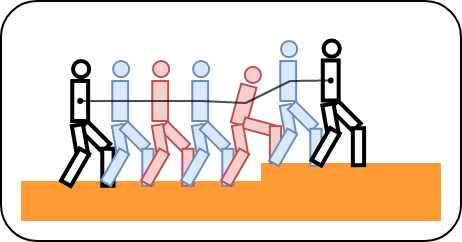
\includegraphics[width=\textwidth]{Figures/Chapter_LEAS/strategies_cp_guide_A.png}
    \caption{Find key contact configurations along the root trajectory\label{fig:strategies_cp_acyclic}}
    \end{subfigure}
    \begin{subfigure}[t]{.49\linewidth}
    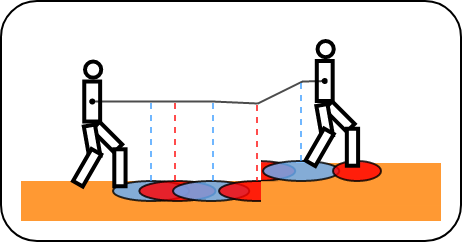
\includegraphics[width=\textwidth]{Figures/Chapter_LEAS/strategies_cp_guide_B.png}
    \caption{Solve the surface selection problem for all steps\label{fig:strategies_cp_mip}}
    \end{subfigure}
    \caption{Contact planner strategies, (a) generates key configurations contact following the root trajectory in input, (b) discretizes the guide to find potential surfaces to step on.}
    \label{fig:strategies_cp}
\end{figure}

The second module $P2$ receives a guide path as input and populates it with a contact sequence. Such a contact planner can have different strategies on how to use the guide. In this thesis, we will explore two strategies for quasi-static contact planning with very distinct problem formulations. 
% Acyclic
The first uses the guide path directly as an exact root trajectory to follow and computes the contacts along it (Figure \ref{fig:strategies_cp_acyclic}).
%The contact planner used in chapter \ref{sec:CP-SB} follows this strategy.
% MIP
The second uses the guide to get some candidate surfaces to step on, then solves a surface selection problem to have exactly one surface selected for each contact (Figure \ref{fig:strategies_cp_mip}).
% Why this decomposition, benefits
The decomposition of the contact planning problem in P1 and P2 (motion-before-contact) breaks the complexity of the contact planning problem, by constraining the search for contacts in the guide path vicinity \cite{AcyclicCP,sl1m_v2}.

Lastly, the module $P3$ performs the contact sequence on the robot with a whole body controller \cite{loco3d, tsid_prete, deepLoco}. For future work, we also implemented an environment to learn such a whole-body controller via deep RL \cite{software_robot_RL}.
In this thesis, we will not use the module $P3$ and focus on the contact planning problem ($P_1$ and $P_2$).


\subsection{Problem Statement\label{subsub:problematic_leas}}

% Motivation
In this context of division into two independent sub-tasks $P1$ and $P2$, the price to pay for the simplification of the contact planning problem is the absence of guarantees of feasibility between the different modules.
In such a sequential framework, the success of a module is a necessary condition for the success of the next in the pipeline but not sufficient.

That is why, to address this issue, some approximations have been made to improve the feasibility of the problem ($P1$) by the next module ($P2$), such as the reachability condition $\mathcal{R}$. The guide path planner assumes that if the ground is reachable at all times along the path, then it is possible to generate a contact sequence. 
This strategy has been proven effective in many scenarios \cite{AcyclicCP}, but can still fail as we will see in the next chapters, weakly approximating the capabilities of the contact planner plugged in. Each contact planner behaves differently as seen in Figure \ref{fig:strategies_cp} and we do not know what makes a feasible guide path for it. As a consequence, it is difficult to define new additional constraints or heuristics in our navigation module ($P1$) to better approximate the contact planning feasibility ($P2$).

% Given the previous context, what do we want ?
We want to fix this issue with a high-level approach, on the very first module of the pipeline $P1$.
The problem we are trying to solve can be formulated as the question: \textit{What is a feasible guide path for a given contact planner ?} 
In other words, how can we build a guide path planner that will better approximate the feasibility space of the contact planner. Such a planner could improve the success rate of $P2$ and sequentially, the success of the whole pipeline.

% Why do we focus on the steering method
As explained previously, $P1$ can be decomposed into two components: a path planning algorithm generating some waypoints to reach, and the SM that sequentially connects these waypoints.
In this thesis, we focus on the steering method that locally generates a guide path between two waypoints.
We want to build an SM able to locally navigate while observing the surrounding terrain to avoid obstacles and validate the reachability condition. 

% Why not working also on path planning ?
% If we have a good SM, then it makes the control a lot more easier for path planning algorithm.
% Path planning algorithm uses the SM to define control points (waypoints) to reach an objective. The SM returns if it succeeded or not to reach this waypoint. A too simple steering method unable to grasp the complexity of the terrain will have a lot of troubles to follow far away waypoints and will makes the search very difficult for the path planning algorithm, requiring more 
The reason why we do not further investigate path planning in this work is that in most simple scenarios, such as walking on flat ground or climbing some stairs, a steering method should be enough to generate a valid trajectory. Doing so also removes the need for a path planning algorithm (RRT, PRM) expensive to compute.
%In the future, the implementation of more efficient path planning algorithm as \cite{RL_RRT} will be implemented.

% What's our solution and why do we use RL for that ?
We build such a terrain-aware steering method with deep Reinforcement Learning (RL).
The choice of using RL is motivated by its capabilities to learn a representation of its environment and to act in it, while maximizing the future cumulative reward and keeping a valid state.
An SM learned by reinforcement could learn how to navigate locally with a vision of its surrounding terrain, while respecting the validity constraints ($\mathcal{R}$ and $\mathcal{C}$) and increasing the success rate of the contact planner.

In this chapter, we first train a pure steering method and provide the results. 
In the next chapters, we use a contact planner as an oracle to validate the trajectories during the learning, then we observe what behavior changes on the SM to increase its success rate.


\section{LEAS: an RL Steering Method\label{subsec:leas-RL}}
% What behaviour do we want for the SM ?
Given initial and goal configurations, we learn by reinforcement a steering method generating a guide path in a given direction while respecting both reachability and collision constraints ($\mathcal{R}$ and $\mathcal{C}$). 
To that end, we designed LEAS \cite{LEAS}, an RL agent that learns by trial and error how to perform this task and to generalize to unknown environments. An overview of our method is presented in figure \ref{fig:LEAS}. The main idea behind LEAS is that for each action taken in the environment, the configuration in $SE(3)$ of the robot will be modified and stored in a list: the guide path.

\begin{figure}
    \centering
    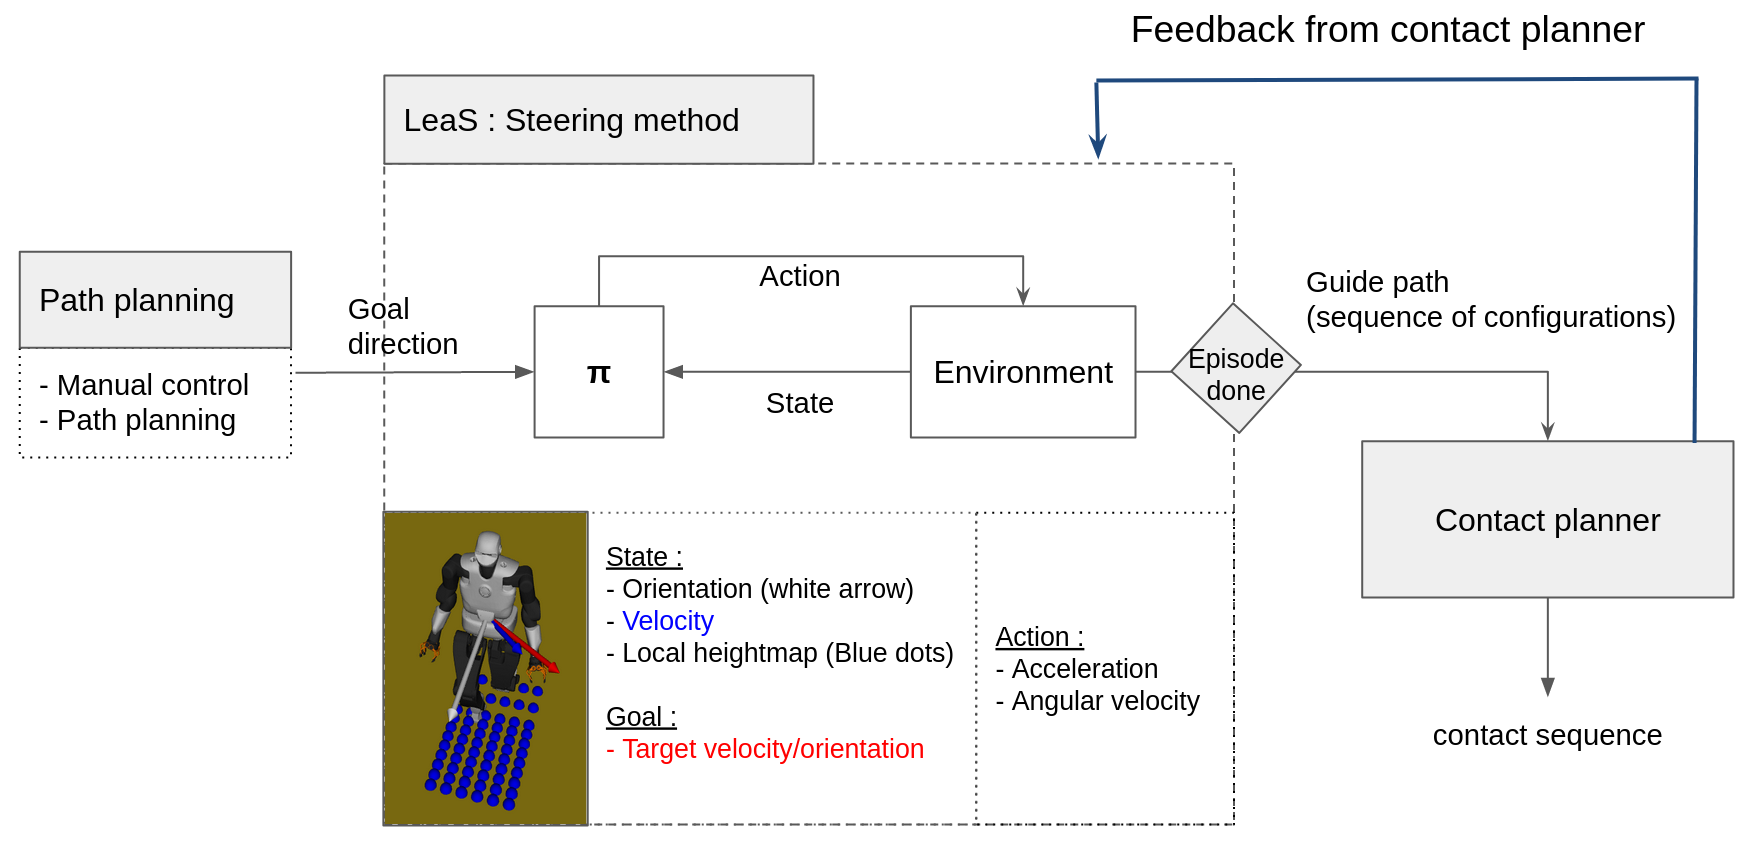
\includegraphics[width=\textwidth]{Figures/Chapter_LEAS/leas_overview.png}
    \caption{Overview of LEAS: the user or a path planning algorithm inputs a target direction to our steering method. LEAS is an RL agent that moves the robot in the environment and sequentially saves all its states. Once the episode is over, this state sequence is the guide path given to the contact planner $P2$. Finally, $P2$ returns an evaluation of the contact plan success that makes LEAS learn how to generate feasible guide paths for it.}
    \label{fig:LEAS}
\end{figure}

In this section, we will take a look at the result of LEAS without plugging it to a contact planner.
Explanations on how LEAS can improve the success rate of a given contact planner will be left for chapters \ref{sec:CP-SB} and \ref{sec:CP-SL1M}.

\subsection{Specifications \label{subsubsec:specifications}}
% What behaviour do we want LEAS to have.
% Goes in depth point by point on every specification of the first sentence, translating it into RL actions/states etc.
We need to specify the task we want to perform with LEAS, with what behavior, and how to achieve it with Reinforcement Learning.

We choose to input a goal direction in LEAS instead of a goal configuration.
We defined a steering method as a planner following a rough path, hence generating a trajectory ending closer to the goal than initially, and that is exactly what LEAS does by moving in the goal direction.
This input also allows for more flexible user controls that can set a fixed goal (reachable or not) in the environment or steer in a direction with a joypad.

Following this design, we desire LEAS to have the following list of behaviours:
\begin{enumerate}[label=(\Alph*)]
  \item Move in the goal direction at a fixed desired velocity.
  \item Respect the reachability and collision constraints, $\mathcal{R}$ and $\mathcal{C}$. 
  \item Stop if it can not go further (i.e keep a valid state).
  \item Navigate locally without the help of path planning, meaning that LEAS should only act based on a very short vision range.
  \item Orientate its root in the desired goal direction. This design choice can be limiting in cluttered environments where side walking is required, but was necessary for our experiments to obtain a straight walk (sidewalking was a predominant locomotion strategy without this specification, as we will discuss in the next chapters).
\label{list:leas:specifications}
\end{enumerate}

The design of an RL agent for our navigation task requires four main components: 
the agent \textit{state} that represents what the agent sees from the environment, the \textit{actions} it performs according to its actual state, the \textit{reward} that evaluates how well the agent acts to achieve the desired behavior, and finally the \textit{done} condition that verifies if an episode is over.

In our work, the \textit{done} condition is straightforward as it verifies the reachability and collision constraints ($\mathcal{R}$ and $\mathcal{C}$), i.e. the episode is over if the actual robot configuration cannot reach the ground or is in collision with the environment. 
Consequently, to maximize the future cumulative rewards, the agent learns by reinforcement how to avoid such cases and to fulfill the behavior (B). 
We can add two optional conditions to stop the episode, depending on the scenario played: when reaching a maximum number of steps, or when being close enough to an objective.





\subsection{States\label{subsubsec:states}}

\begin{figure}[ht]
    \centering
    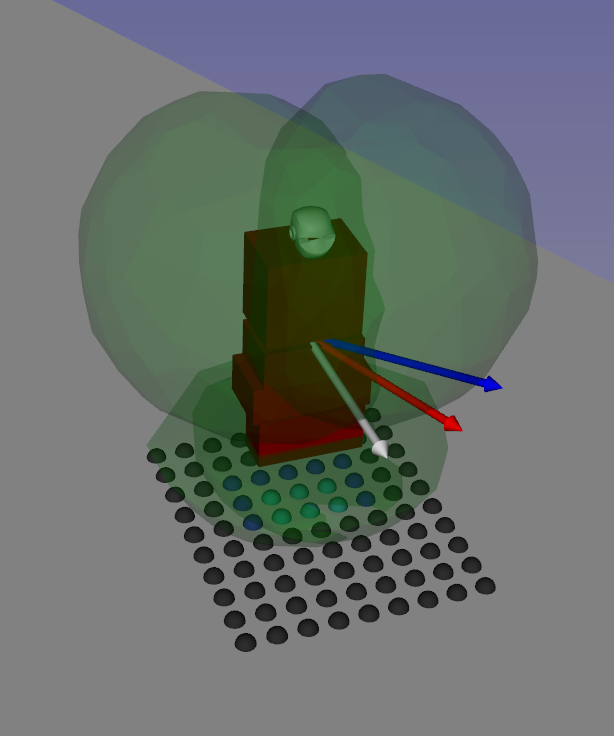
\includegraphics[width=0.42\textwidth]{Figures/Chapter_LEAS/leas_states.png}
    \caption{Robot states: (blue arrow) velocity of the robot, (white arrow) orientation, (red arrow) desired velocity and orientation, (dots) height map relative to the root configuration.}
    \label{fig:LEAS_states}
\end{figure}

The robot configuration can be seen in figure \ref{fig:LEAS_states}, from which we can get the observable states driving the actions of LEAS. The desired velocity and orientation are represented by the same vector and expressed implicitly in our states.

The observable state is a set: 
\begin{equation}
s=\{v_{o}, o_{target}, h_{o}\}
\end{equation}
with $v_{0}$ the velocity of the robot relative to its orientation, $o_{target}$ the angle between its actual and desired orientations (yaw), and $h_{o}$ a local height map of the terrain relative to its root configuration.

\begin{figure}[t]
    \captionsetup[subfigure]{justification=centering}
    %\centering
    \begin{subfigure}[t]{.49\linewidth}
    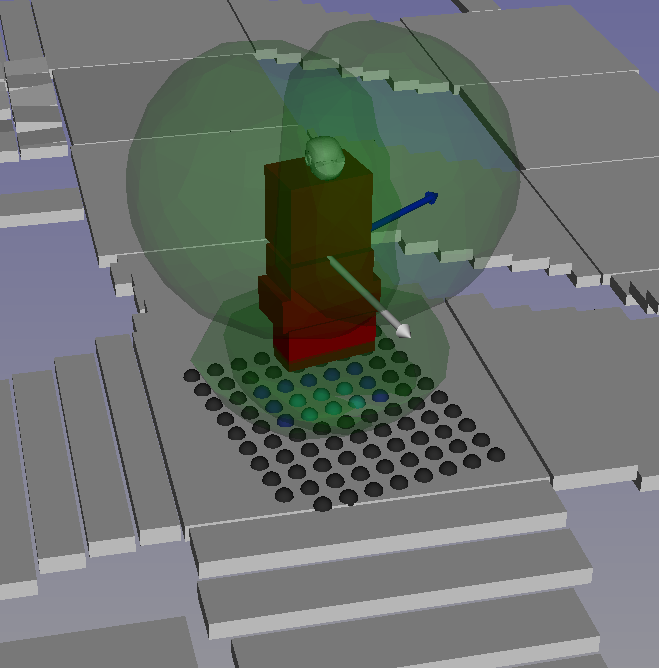
\includegraphics[width=\textwidth]{Figures/Chapter_LEAS/hm_small_vision.png}
    \caption{\label{fig:vision_hm_size_short}}
    \end{subfigure}
    \begin{subfigure}[t]{.49\linewidth}
    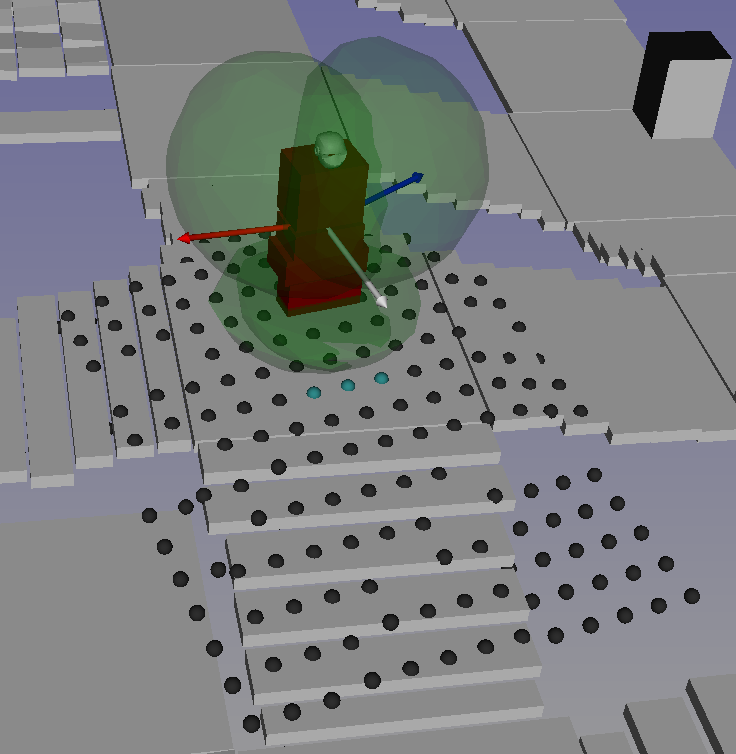
\includegraphics[width=\textwidth]{Figures/Chapter_LEAS/hm_big_vision.png}
    \caption{\label{fig:vision_hm_size_big}}
    \end{subfigure}
    \caption{Vision field of LEAS for different local height map sizes.}
    \label{fig:vision_hm_size}
\end{figure}

% - height map for the agent to understand locally its surrounding. 
% Explain the dimensions, the number of dots, the space between them. 
The dimensions of the height map are 7 values in front of the robot, 3 in the back, and 7 values on each side with a discretization step (rounded) of $15$ cm, $17$ cm, and $9$ cm respectively. This roughly corresponds to a short vision range of $110$ cm in the front, $50$ cm in the back, and $60$ cm on each side of the robot (figure \ref{fig:vision_hm_size_short}).

% Why not bigger ?
The observable height map is small on purpose as we desire a steering method with the behavior (D), to navigate locally. Increasing its visual field leads to an over-fitting on our training terrain and the emergence of path planning behavior.
Indeed, if we give too much information about the surrounding terrain (figure \ref{fig:vision_hm_size_big}), one could memorize its topography, guess its global position on it and plan its path through it, as done in \cite{rl_navigation_video_game_2020}.
Empirically, we found that $110$ cm in front and $60$ cm on each side of the robot was enough for LEAS to detect the obstacles and react in consequence.
% Is this discretization enough ?
The height map resolution of LEAS is $15$ cm, compared to previous works as \cite{RLOC, deepGait, deepLoco} that have a resolution of 2cm, 4cm, and 34cm respectively, and is sufficient to navigate the training ground and to generalize to unknown terrains. 
Increasing its resolution did not improve the learning or navigation skill of LEAS for our test scenarios, but may be required in the future for more complex scenes with elements of smaller surfaces (handrails detection for example).

\begin{figure}
    \captionsetup[subfigure]{justification=centering}
    %\centering
    \begin{subfigure}[t]{.49\linewidth}
    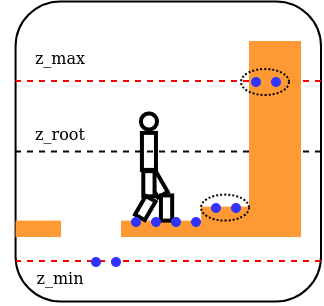
\includegraphics[width=\textwidth]{Figures/Chapter_LEAS/hm_bounded_high.png}
    \caption{Wide height map bounds}
    \end{subfigure}
    \begin{subfigure}[t]{.49\linewidth}
    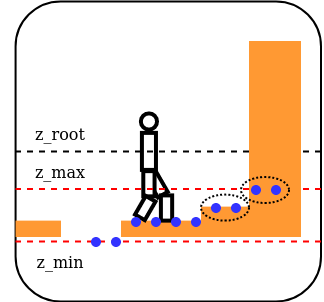
\includegraphics[width=\textwidth]{Figures/Chapter_LEAS/hm_bounded_low.png}
    \caption{Small height map bounds}
    \end{subfigure}
    \caption{Observable height map with $z_{min}$ and  $z_{max}$ relative to $z_{root}$ and (blue dot) the bounded height map values. If these bounds are (a) too large, the agent can easily detect the distant obstacle but may not dissociate the ground and the stair in front of him, or (b) too tight, the agent can better detect it but mistake the obstacle as a second stair.}
    \label{fig:height map_bounds}
\end{figure}

% What are the bounds for this relative height map ? Why not bigger bounds ?
All $z$ values in the local height map are bounded between $[z_{min}, z_{max}]$. 
The tuning of these bounds depends on the topography of the terrain where LEAS will navigate. 
Indeed, a wider interval means that the RL agents will better dissociate higher height variations (stairs and obstacles) at the cost of a lower resolution for small variations (rubbles and small slopes).
This is illustrated in figure \ref{fig:height map_bounds} where wider bounds (a) are a better representation for obstacle detection, and smaller bounds (b) make the agent more sensitive to small height variations but may mistake the distant obstacle as a stair. 
Empirically, we find a right balance $z_{max}= -0.2$ and $z_{min}= -1.4$ meters from the robot root (usually located at 1 meter from the ground), to be sufficient for LEAS to visualize both small and high variations during a pure navigation task.

\subsection{Actions\label{subsubsec:actions}}
At each step, the RL agent takes action in the environment based on the observed state. 
Our policy returns a set of actions: 
\begin{equation}
a = \{ a_x, a_y, a_z, \omega \}
\end{equation}
with $a_x, a_y, a_z$ the accelerations of the robot on each axis, and $\omega$ the angular velocity of the robot on the yaw axis. At each step $i$, the robot position q$_{pos}$, velocity q$_{vel}$ and orientation q$_{ori}$ are modified in the following order:
\begin{equation}
\begin{cases}
(a) \; q_{pos}^i = q_{pos}^{i-1} + q_{vel}^{i-1} * T \\

(b) \; q_{vel}^i = q_{vel}^{i-1} + [a_x, a_y, a_z] * T \\

(c) \; q_{ori}^i = q_{ori}^{i-1} + \omega * T 
\end{cases}
\end{equation}
with $T$, a user-defined timestep, q$_{pos}$, q$_{vel}$, and q$_{ori}$ the global position, velocity, and orientation of the robot respectively.

The velocity $q_{vel}$ and timestep $T$ impact the number of configurations along the guide path. For a constant velocity along the guide of $0.10$ m/s and $T=0.2$ seconds, the discretization step between each configuration is $2$ cm. 
We can further bound q$_{vel}$ in order to keep its norm $|\mbox{q}_{vel}| \leq v_{max}$ with $v_{max}=0.2$ m/s. %All parameters can be seen in Table \ref{tab:param}.

The choice of $T$ depends on the contact planner used. 
Empirically, we know that the contact planner \cite{AcyclicCP} has a higher success rate for discretization steps inferior to $15$ cm.
For LEAS, we choose to set $T=0.2$ seconds which results for $v_{max}=0.2$ m/s in a maximum discretization step of $4$ cm.
In the next chapters, we will further prune configurations along the guide to modify this maximum discretization step when required.
These parameters have been empirically selected to achieve the specified navigation behaviors, while computing enough configurations along the guide to be feasible by our contact planners (discussed in the next chapters).

% Why this order for the control in acceleration ? It induces a delay in the action
The order in which the robot states are updated induces a delay in the action of the agent. 
The position of the robot is updated with the previous velocity (1), then the acceleration actions update the velocity (2). As a result, the agent can observe its action impacts directly on the velocity, but not on the robot position and so its observable local height map.
%In RL, problems where the actions are not instantly applied to the states or captured by the observations have been termed as Delayed MDPs \cite{RL_delayed}. 
%Our control does not fall directly into this category as the agent can see its actions directly on the velocity. 
One can ask if inverting the order of (1) and (2), hence removing this delay on the position could improve the learning and results of our agent. 
In practice with recent RL algorithms, fixed delays of one or two steps do not matter \cite{RL_delayed_explanation} as long as the agent has enough steps left to react to an event. We verify it in figure \ref{fig:control_LEAS_learning_curves} that shows no difference in the learning of both controls with our parameters.

% Controls: why control in acceleration ?
We choose an acceleration control for LEAS, where velocity changes along the trajectory are limited by $a_{max}$, the maximum acceleration.
In our experiments, we find that small accelerations with a small timestep $T$ help the exploration and lead to a more stable training overall, as the actions have a lower impact on the system compared to a velocity control.
That is why we set a sufficiently high maximum acceleration $a_{max}=0.08$ m/s$^2$ to react to new observations, as the detection of an obstacle, but low enough to help its learning and generate smooth trajectories.

% Why not just giving the configs for each step ?
Another option is position control, where the actions directly correspond to the next root position $q_{pos}$, or similarly velocity control with a high timestep $T$, to exactly compute one configuration per footstep along the guide.
% Removed: In our experiments, this implementation does not work well with our sample-based contact planner of chapter \ref{sec:CP-SB} that prefers guide paths with a small discretization step, but is pertinent for those of chapter \ref{sec:CP-MIP} and \ref{sec:CP-SL1M}. 
While this strategy is pertinent in the contact planning context, it is also more difficult to train as it requires a few numbers but critical actions to generate a guide path.
In our experiment, training LEAS with such position control is inefficient as it drastically lowers the probability to end in a feasible state, hence requiring additional strategies to guide the exploration.
As a consequence, we prefer an acceleration control leading to stable learning of our navigation task. 
%However, this approach also implies additional implementation choices relative to the contact planners that will be discussed in the next chapters.

\subsection{Rewards}
% What do we want our robot to do ?
As written in the specifications (section \ref{subsubsec:specifications}), the behaviors we have yet to obtain are: (A) move the robot in the goal direction at the desired velocity, (C) stop if it can not go further, (E) orientate its root in the goal direction. 
We design three rewards to get these behaviors:
\begin{enumerate}
  \item[(E)] $R_{ori} = -( 1 -  \overrightarrow{q_{ori}} \cdot \overrightarrow{u}_{target} )$ \\
  with $\overrightarrow{q_{ori}}$ the unit vector representing the root orientation and $\overrightarrow{u}_{target}$ the goal direction.
  \item[(A)] $R_{dir} = -( ||\overrightarrow{q_{vel}} - \overrightarrow{v*} ||/(2v_{max}) )^2$\\
  with $\overrightarrow{q_{vel}}$ the root velocity vector, $\overrightarrow{v*}=\overrightarrow{u}_{target} \times v_{desired}$ the desired velocity vector and $v_{max}$ the maximum velocity norm.
  \item[(C)] $R_{alive} = 1$ 
    %$
    %\begin{cases}
    %  1, & \text{if the actual state is valid} \\
    %  0, & \text{otherwise}
    %\end{cases}
    %$
\end{enumerate}
The reward $R_{ori}$ penalizes the agent for not being oriented toward the goal (E) and $R_{dir}$ penalizes it for not moving in the desired direction at $v_{desired}$ (A). 
As both rewards are negative, using only these two encourages the agent to terminate the episode as soon as possible to avoid accumulating negative rewards. 
Therefore, we introduce another positive constant reward $R_{alive}$ that the agent gets at each step to encourage him to keep a valid configuration and continue the episode.
As a result, the agent learns that to maximize the future rewards, if it is not possible to move in the desired direction, it is better to keep the robot idle rather than terminate the episode, thus fulfilling the behavior (C).

To further smooth the trajectory, we add two rewards to punish the agent for taking large actions:
\begin{enumerate}
    \item $R_{\omega} = - | \omega / \omega_{max} |^2 $ \\
    with $\omega$ the action on orientation and $\omega_{max}$ the maximum angular velocity.
    \item $R_{acc} = - (|| [a_{x},a_{y},a_{z}] || / a_{max})^2 $ \\
    with $[a_{x},a_{y},a_{z}]$ the acceleration actions and $a_{max}$ the maximum acceleration norm.
\end{enumerate}

The resulting reward is :
$R = R_{dir} w_{dir} + R_{ori} w_{ori} + R_{\omega} w_{\omega} + R_{acc} w_{acc} + R_{alive} w_{alive}$\\
with $w_{dir}$, $w_{ori}$, $w_{\omega}$, $w_{acc}$ and $w_{alive}$ some user-specified weights.

\hfill %\break

Another possible reward design is to let $R_{dir}$ be positive as done for the High-level controller of DeepLoco \cite{deepLoco}. 
For example, we can set $R_{dir}=-(||\overrightarrow{v} - \overrightarrow{v*}||/(2 v_{max}))^2 + 1$ and remove $R_{alive}$, which in that case is strictly equivalent to our formulation above with $R_{alive}=1$ and $w_{alive}=1$.
That is why for more convenience, we separate these two rewards. 
An advantage of this separation is that we can increase $w_{alive}$, relative to the other reward weights, to further force the agent to act carefully and stay away from dangerous situations like staying too close to an obstacle. 
In our experiments, keeping $w_{alive}=1$ is sufficient to get the desired behavior (C), but setting it too high as $w_{alive}=2$ can make the agent act too safely and stay idle instead of crossing difficult obstacles.

\section{Implementation Details\label{subsec:leas-implementation}}

% Problem with using HPP like that:
% - HPP is made for scenarios on small scenes with a low number of surfaces
% - HPP can run several clients, but main use: perform scenario, close it, then restart it. No easy reset.
% - Very slow to load big scenes
% - No tool to get the height map
% - The scenes are fixed and we can not change it => One instance = one scene
% - Functions of HPP are done in C++ (fast), but may be slower if intensively called again and again as configuration validity => Need a better way to check validity (collision+reachability) => Approximations using HM.

We train LEAS using HPP software \cite{HPP} to load the terrain and the Talos robot model \cite{talos_robot}. 
To speed up the training process and learn a policy with good generalization capabilities, it is desirable to have several agents in parallel during the training to generate trajectories on one or several diverse scenes.
% Limit of HPP
While it is possible to have several clients of HPP on the same machine, this software was mainly implemented for short scenarios on small terrains, but not for intensive usage as we do in RL or to load scenes with thousands of surfaces. 

To that end, we implemented a python library to extract a height map from the scene meshes, and we present two main tools to be implemented in HPP later on: an approximation of the collision and reachability constraints using the height map, and a random terrain generator. 
Finally, we present an asynchronous version of the RL algorithm Proximal Policy Optimization (PPO) \cite{PPO_2017} that will be used in the next chapters to externally compute the contact planning sequence with a master-workers architecture.

\subsection{Validity Approximation\label{subsub:validity_approximation}}
% Explain how it is done in HPP
% Why the need to approximate it => Remove dependencies with HPP that was made for smaller scenes + Faster and simplified, enough for LeaS.
% I approximated the ROM => bounds for each point on the rel HM. Easier to tune it, without needing to cut the ROM files.
% Reachability: If all points of ROM on rel HM bellow bounds => unreachable.
% Stricter reachability: points of ROM (middle) must be above bounds.
% Collision: If one above on mid point of rel HM above bounds => collision.
The validity of a configuration is subject to two constraints: reachability $\mathcal{R}$ and collision $\mathcal{C}$.
Efficient functions are available in HPP to verify these constraints by checking if an intersection exists between either the range of motion of the robot legs or the volume representing its trunk, and the terrain surfaces. 
However, in our first version of LEAS \cite{LEAS}, the computation time of these validation functions was significant (more than 15\% of the computation time), and as a consequence, we opted for a faster and more flexible implementation of these constraints.

\begin{figure}[ht]
    \captionsetup[subfigure]{justification=centering}
    \centering
    \begin{subfigure}[t]{.35\linewidth}
    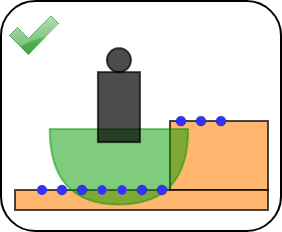
\includegraphics[width=\textwidth, height=4cm]{Figures/Chapter_LEAS/approx0.png}
    \caption{\label{fig:approximation_validity_0}}
    \end{subfigure}
    \begin{subfigure}[t]{.35\linewidth}
    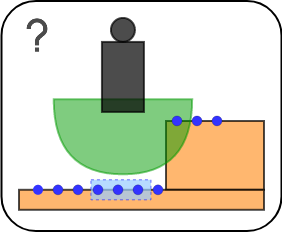
\includegraphics[width=\textwidth, height=4cm]{Figures/Chapter_LEAS/approx1.png}
    \caption{\label{fig:approximation_validity_1}}
    \end{subfigure}
    \begin{subfigure}[t]{.35\linewidth}
    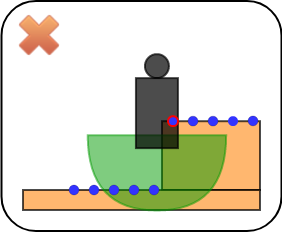
\includegraphics[width=\textwidth, height=4cm]{Figures/Chapter_LEAS/approx2.png}
    \caption{\label{fig:approximation_validity_2}}
    \end{subfigure}
    \begin{subfigure}[t]{.35\linewidth}
    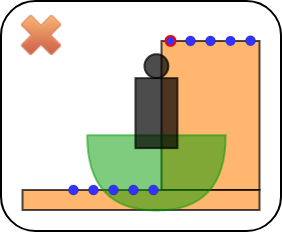
\includegraphics[width=\textwidth, height=4cm]{Figures/Chapter_LEAS/approx3.png}
    \caption{\label{fig:approximation_validity_3}}
    \end{subfigure}
    \caption{Approximated validity conditions: (Green) robot range of motion, (blue) height map. Configuration (a) is valid, (b) is valid with $\tilde{\mathcal{C}}$ and $\tilde{\mathcal{R}}$ but invalid with $\tilde{\mathcal{R}^*}$ where none of the highlighted blue dots are reachable, (c) and (d) are valid with $\tilde{\mathcal{R}^*}$ but in collision.}
    \label{fig:approximation_validity}
\end{figure}

We approximate the collision and reachability constraints by $\tilde{\mathcal{R}} \subset \mathcal{R}$ and $\tilde{\mathcal{C}} \subset \mathcal{C}$ respectively, both using the local height map $H$ relative to the robot root (Figure \ref{fig:approximation_validity}).
Offline, we assign to each point $p_i \in H$, some reachability $\tilde{\mathcal{R}_i}$ and collision $\tilde{\mathcal{C}_i}$ constraints on its height $z_i$. 
A point $p_i$ respects $\tilde{\mathcal{R}_i}$ if it lies inside the robot range of motion, and respects $\tilde{\mathcal{C}_i}$ if it lies outside and under the robot trunk volume. 
The approximated reachability condition is valid if:
\begin{equation}
    H \in \tilde{\mathcal{R}} \Rightarrow \exists p_i \in H, p_i \in \tilde{\mathcal{R}_i}
\end{equation}
The approximated collision condition is valid if:
\begin{equation}
    H \in \tilde{\mathcal{C}} \Rightarrow \forall p_i \in H, p_i \in \tilde{\mathcal{C}_i}
\end{equation}
These approximations require the robot root to only rotate on the yaw axis when navigating, that is a common assumption for biped locomotion \cite{deits2014FootPlanMI}.

One drawback of using a single-layer height map for this validity condition is its limitation to environments without an upper floor or ceiling.
% Collision detection
Regarding $\tilde{\mathcal{C}}$ constraint, the trivial case is that if a point $p_i$ lies inside this volume, there is a collision (figure \ref{fig:approximation_validity_2}). However, we do not know if there is a collision if a $p_i$ lies right above the robot. 
There are two cases: first, the robot is under an object (ceiling) and not in collision; second, the robot is inside the object (e.g. wall) and so is in collision (figure \ref{fig:approximation_validity_3}).
From the height map, we cannot distinguish these cases and thus we choose to consider both as a collision.
% Conclusion of this drawback
As all our test terrains do not contain an upper floor and we do not perform any locomotion task like passing under a gate, such an approximation is sufficient. 
In the future, another solution will be required to navigate such scenes like using a two-layers height map or voxels to better approximate the terrain geometry or using alternative validity conditions.

% No longer true with the formulation above
% is that it considers upper floors and ceilings as obstacles. However as we do not perform scenarios as passing under a gate or crouching to move under a low ceiling, such approximation is acceptable. A solution to this limitation in a future work could be to use two height maps, one for the closest ground floor and a second one for the upper ceiling.  \stn{ou simplement pas mettre le pied plus haut que le torse ?}

% Depending on the discretization of the height map, it can happen that the reachability constraint is not fulfilled even if graphically, we can see that the ground is reachable. 
% If a config is invalid with the approx, recheck :
% (1st option) Use isConfigValid of HPP.
% (2nd option) Create a convex hull from the approximated reachability bounds, and check if there is an intersection with any of the potential surfaces
Another limitation comes from the height map resolution that can fail to approximate the constraints $\mathcal{R}$ and $\mathcal{C}$.
% What happens
% Reachability
On reachability, a low height map resolution can fail to visualize a scene composed of small and spaced surfaces. Consequently, it can wrongly consider that $H \notin \tilde{\mathcal{R}}$ (i.e. the terrain under the robot is not reachable) when in reality $H \in \mathcal{R}$.
To remove such cases, we can reconfirm the invalidity of the configuration with the full constraint $\mathcal{R}$, resulting in a reasonable trade-off between computation time and completeness.
% Collision
As for the collisions, the opposite can happen where a collision is not detected by the approximation, $H \in \tilde{\mathcal{C}}$, when in reality $H \notin \mathcal{C}$. Consequently, only the full validation $\mathcal{C}$ can detect these cases.
In practice, our steering method learns to keep a safe margin between the obstacles and the robot trunk to avoid collisions and so, implicitly avoid these collision detection failures. 
Therefore, we choose to rely on the approximated constraint $\tilde{\mathcal{C}}$ that is sufficient to detect most of our robot trunk collisions.
% Trade-off
%In our implementation, we opt for a trade-off between the fast to compute approximated validity constraints $\tilde{\mathcal{R}}$ and $\tilde{\mathcal{C}}$ checked at every step of the guide path generation, where the full reachability condition $\tilde{\mathcal{R}}$ is only performed to confirm the invalidity of a root configuration.
\begin{figure}[ht]
    \centering
    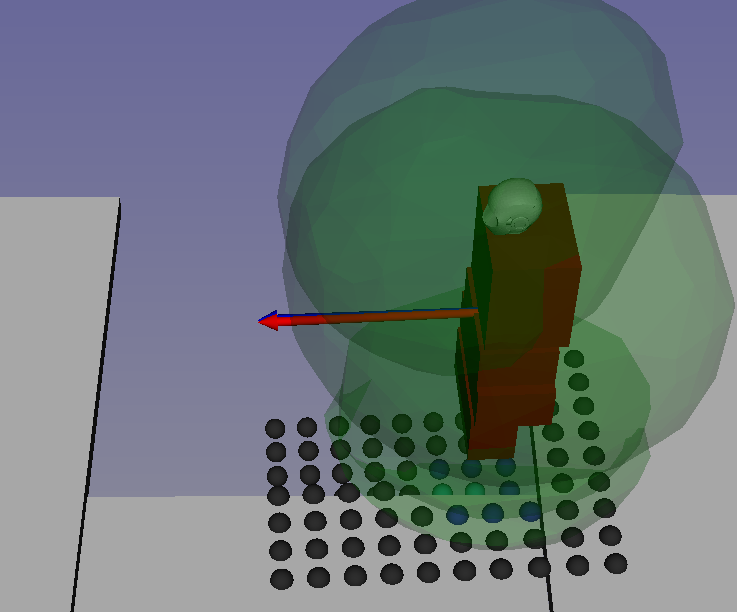
\includegraphics[width=0.42\textwidth,height=4.5cm]{Figures/Chapter_LEAS/hole_scenario_above_void_p1.png}
    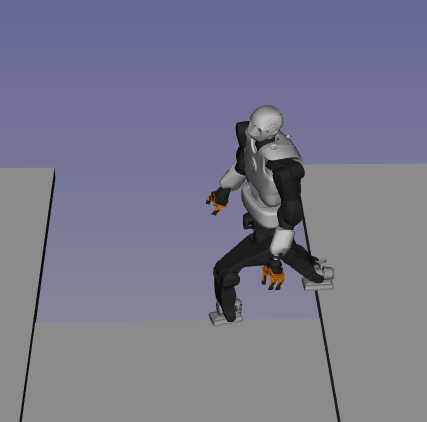
\includegraphics[width=0.42\textwidth,height=4.5cm]{Figures/Chapter_LEAS/hole_scenario_above_void.png}
    \caption{Valid configuration with $\tilde{\mathcal{C}}$ and $\tilde{\mathcal{R}}$ leading to a blocking configuration above the hole.}
    \label{fig:hole_scenario_above_void}
\end{figure}

Finally, we add one additional constraint to further improve the guide quality for the biped locomotion task. 
One default of the original validity function is that configurations above the void but touching the edge of the terrain with the range of motion are considered valid (Figure \ref{fig:hole_scenario_above_void}), leading to infeasible trajectories by our contact planners.
To avoid these configurations, we add another validity condition on the height map $H^*$ located directly under the root of the robot to be reachable at all times (dots under the robot in Figure \ref{fig:approximation_validity_1}). 
We name the reachability constraint with the stricter condition $\tilde{\mathcal{R}^*}$ where:
\begin{equation}
    H \in \tilde{\mathcal{R}^*} \Rightarrow \exists p_i \in H^*, p_i \in \tilde{\mathcal{R}_i}
\end{equation}
With this strategy, configurations are considered invalid if the robot stands above the void. 
It can be limited on terrains with very spaced surfaces, but in all our scenarios this condition offers good results in terms of guide path quality.
This solution was not yet implemented in our first version of LEAS \cite{LEAS} where we learned by reinforcement such additional constraints using the contact planner as a guide path validator, hence leading to longer training.
%This leads to the generation of a guide path with fewer states above the void and so a faster computation time with our contact planners.

In the context of RL, where the agents perform millions of steps, the approximations $\tilde{\mathcal{R}^*}$ and $\tilde{\mathcal{C}}$ significantly improve the training time.
While the gains in computation can not be fairly compared due to their difference in programming language and optimization, our implementation resulted in an average of 20 times faster computation time compared to the full constraints $\mathcal{R}$ and $\mathcal{C}$, hence enabling us to train and test more models.

\subsection{Terrain Generator\label{subsub:terrain_generator}}

\begin{figure}[ht]
    \centering
    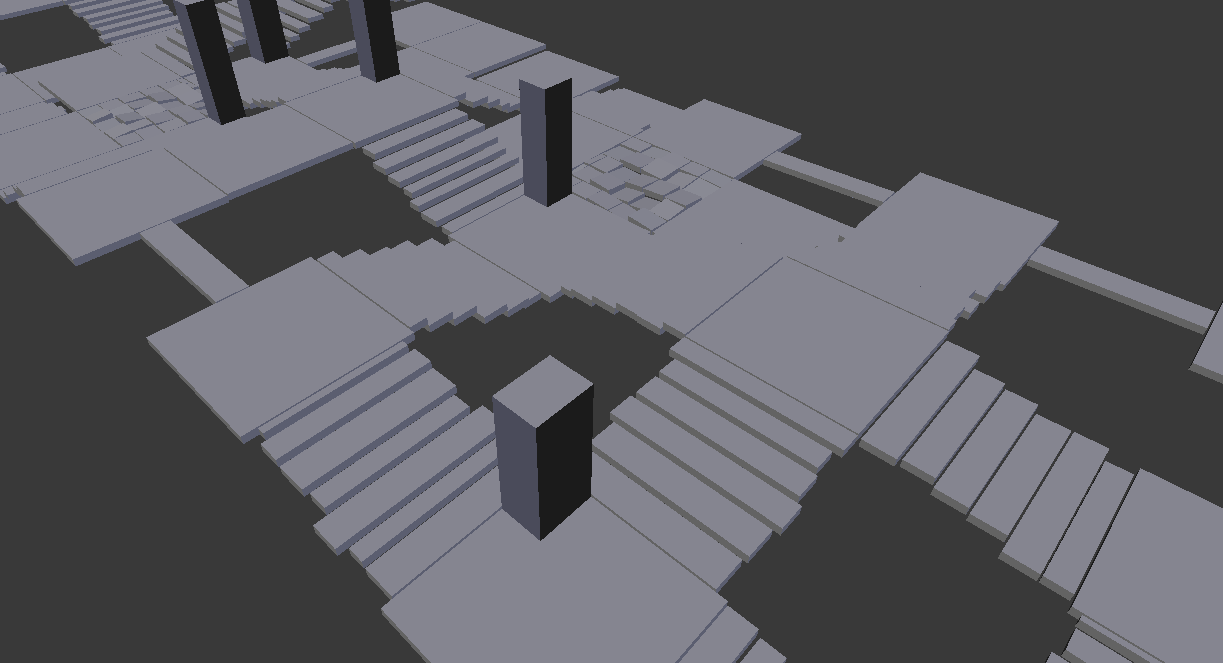
\includegraphics[width=0.7\textwidth]{Figures/Chapter_LEAS/random_scene_tiles_example.png}
    \caption{Example of a random scene generated, containing different types of tiles connected. Initial tiles: flat ground with and without obstacles. Transition tiles: rubbles, bridge, and stairs.}
    \label{fig:random_scene_gene_tiles_example}
\end{figure}

% Originally made by daeun, and adapted by me to produce arenas of size NxM
% That is somehow a huge part of my work that was needed for LeaS.
% Give a link to the code as well, but say that some fix need to be made.
Our goal is to train one policy to navigate through all our test scenarios.
To improve its generalization capability, our RL agent has to learn on various terrains. 
To that end, we extended the library used in \cite{sl1m_v2} to generate random terrains composed of rubbles, stairs, bridges, and obstacles. The code is available on GitHub \cite{random_scene_gen}.

This library generates a terrain that we can divide into tiles. 
Each tile belong to two categories: \textit{Initial} or \textit{Transition} (figure \ref{fig:random_scene_gene_tiles_example}). 
The first category \textit{Initial} contains two types of tiles: flat ground with or without obstacles. 
The second category \textit{Transition} connects two \textit{Initial} tiles and contains three types: rubbles, bridge and stairs.

We represent the terrain as a grid where each cell is a fixed-sized tile. Starting from an \textit{Initial} tile, we build a tree filling pseudo-randomly its empty neighbors. Each \textit{Transition} is unique as the characteristics of each surface composing it are random, but also depend on the height of the tiles it connects.

At the end of the terrain generation, we can identify all the links created. 
A link is defined as a sequence of \textit{Initial} - \textit{Transition} - \textit{Initial} tiles in a line, and that we can further divide into several categories in function of their difficulty. 
Finally, we extract the possible starting positions for the robot on each link, corresponding to areas on the \textit{Initial} tiles. 

Terrains generated by this library can contain enough elements, depending on the grid dimension and the random seed, for the agent to develop its navigation skill, then generalize to our test scenes that contain the same type of transitions.



% Some limitations of using this library to generate terrains for the training
% (1) All tiles have the same size, it can be a problem depending on the observable height map of the agent, for example, it will never learn how to climb very long stairs if the hm is too big.
% (2) It is limited to the kind of transitions that are implemented. Very different obstacles as walking on plateforms or weird scenarios may not work with an agent trained on our terrain. Even though our arena is big and contains enough element for the agent to figure out most of our test scenarios.
% (3) These scenes are still fixed, no dynamic elements. Ok for our test scenarios.
% (4) The quality of the agent depends on the scene it's been trained on. We have to carefully see if the generated scene contain enough of each tile types.
Some limitations come with the use of this library for our training.
The first is that all the tiles have the same dimensions, fixed to 2x2 meters for all our training scenes. 
Its dimensions have to be carefully tuned according to the size of the observable height map by the agent.
Indeed, a too large visual field could lead the agent to specialize in navigating scenes with this specific tile size, e.g. the agents can specialize in crossing stairs or bridges of 2 meters. 
In our experiments, with a visual field of $110$ cm in the front (Section \ref{subsubsec:states}), learning on a terrain of 2x2 meters tiles is sufficient to learn local navigation behaviors.
The second limitation is that even though the \textit{Transition} and obstacle tiles are unique and randomized, they still fall into the same categories (i.e. stairs, rubbles, bridge, obstacle). Consequently, we could question the ability of the agent to navigate on very different terrains. Empirically, this was not a problem to generalize to all our test scenarios mostly containing the same type of elements, however, a higher diversity may be required in the future.
The performance of the agent also depends on the size of the terrain it has been trained on. We had to generate several random arenas before finding one having enough elements and links. 
In our experiments, terrains of dimension 5x30 are the maximum we can have in HPP as the terrain loading and processing times exponentially increase with the number of surfaces.

% Options tried
% (1) All parallel agents during the training evolves on different terrain, possibility to change this terrain, going from an easy one first to a more difficult one later on => Curriculum learning. Then we run one or several contact planners for each type of terrain, that will compute the CP only for these terrains.
% (2) Have just one huge scene that has enough diversity of obstacles / transitions to learn how to generalize.
% A combination of (1) and (2) is also possible.
 Finally, several options can be explored to learn from the random scenes generated.
 We can have several parallel agents learning in different scenes or modifying the scene during the training.
 We can also use the difficulties of each link in the scene to perform curriculum learning \cite{curriculum_learning_survey}, starting from the easiest link to the most difficult one.
 In a previous test, we ran several agents during the training on different terrains and following such a curriculum learning, for example starting from flat ground, then switching to stairs, and finally, a terrain randomly generated. However, it did not further improve the learning time, as our agent is already able to learn quickly from a single 5x30 random scene without these methods.
 
 
\subsection{Master-Workers Architecture: Asynchronous contact planners\label{subsub:leas:master_worker}}

% Why did I pick PPO (online) and not an offline RL algo
Several state-of-the-art RL algorithms are available and can be separated into different groups, each presenting some pros and cons, and that can lead to various results depending on their hyperparameter tuning and the task to perform \cite{RL_that_matters, RL_that_matters_OnPolicy}. As a consequence, it can be difficult to judge which algorithm to use for a given task other than empirically. 
%However, some comparisons are available to guide our choice \cite{compare_PPO_TD3_SAC_DDPG}.
Among the most recent and popular RL algorithms, we have Proximal Policy Optimization (PPO) \cite{PPO_2017} in the category of on-policy algorithms, and Twin Delayed DDPG (TD3) \cite{TD3_2018} and Soft Actor-Critic \cite{SAC_2018} in off-policy.
% What do we try ?

In this work, we experimented on PPO and TD3, both implemented in Stable Baseline \cite{stable-baselines} that we can easily adapt for our task.
% What are the main pros and cons
Off-policy algorithms, such as TD3 and SAC, are known to be more sample efficient but can lack stability compare to on-policy RL algorithms.
% What do we pick in the end ?
% Note: TD3 is hard to tune, it did not converge after 3M steps, when PPO already converged.}
That is why many recent works in RL use PPO \cite{survey_rl_animation_pettre_2022} that, to this day, can be easier to tune and more stable during the learning, even for tasks that require data-efficiency as \cite{openai2019dota}.
%The learning of LEAS without a contact planner, which is a pure navigation task can be learned efficiently with PPO as in \cite{compare_PPO_TD3_SAC_DDPG} for a boat navigation task.
In our first version of LEAS \cite{LEAS}, the training with PPO was slow due to its poor sample efficiency (order of hours without contact planning and tens of hours with our sample-based contact planner). %At that time, using off-policy RL algorithms was a more pertinent choice.
However, this issue was fixed with the optimizations and approximations discussed in the previous section thus making both off- and on-policy pertinent choices.
We tested TD3 and PPO for our navigation task and we observed with TD3 a slower and less stable convergence than PPO, using the default hyperparameters as defined in Stable Baseline or with manual tuning.
As a result, we decided to use PPO to learn LEAS.

% What is the main problem of LEAS design, how to modify PPO to make it works ?
% Why only asynchronous for the CP ? Why master-worker ? Are there some limitations / alternatives ? => Limitation of our software + exchange of datas between processes + the CP is the only long thing to compute and just need the guide path to be done.
Given the design of LEAS, we have two components to consider during the training. First, our steering method is a policy taking actions in the environment and saving the state sequence as a guide path. Second, the contact planner computes the contact sequence along it and gives feedback on its result to LEAS.
%We do not define the feedback in this section that depends on the contact planner used and the type of reward we want to implement.
In this design, the main limitation comes from the contact planning validation at the end of each episode. 
If we simply perform this contact planning inside each agent, as all parallel agents are steps synchronous (or trajectory synchronous), if one agent computes a contact sequence, all the others have to wait for it to finish. Consequently, the computation time increases with the number of agents in parallel.
We have two solutions to solve this problem: (a) Compute all trajectories asynchronously or (b) compute all guide paths synchronously and perform P2 asynchronously.
We implemented both solutions (a) and (b) using a master-worker architecture (Figure \ref{fig:architecture_master_worker}).
\begin{figure}[t]
    \captionsetup[subfigure]{justification=centering}
    %\centering
    \begin{subfigure}[t]{0.9\linewidth}
    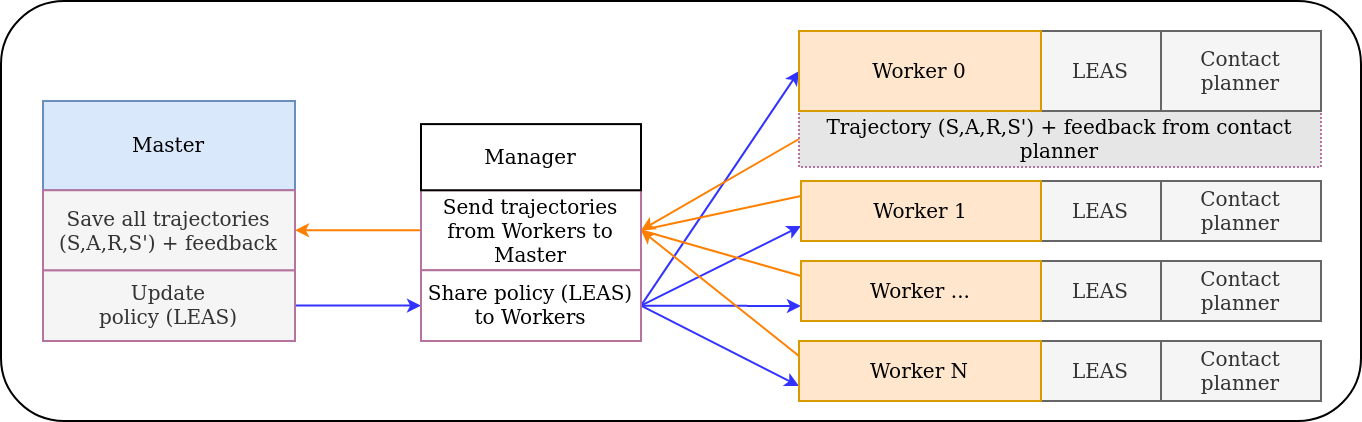
\includegraphics[width=\textwidth]{Figures/Chapter_LEAS/architecture_master_worker_0.png}
    \caption{Asynchronous guide path and contact planning}
    \label{fig:architecture_master_worker_synchronous}
    \end{subfigure}
    \begin{subfigure}[t]{0.9\linewidth}
    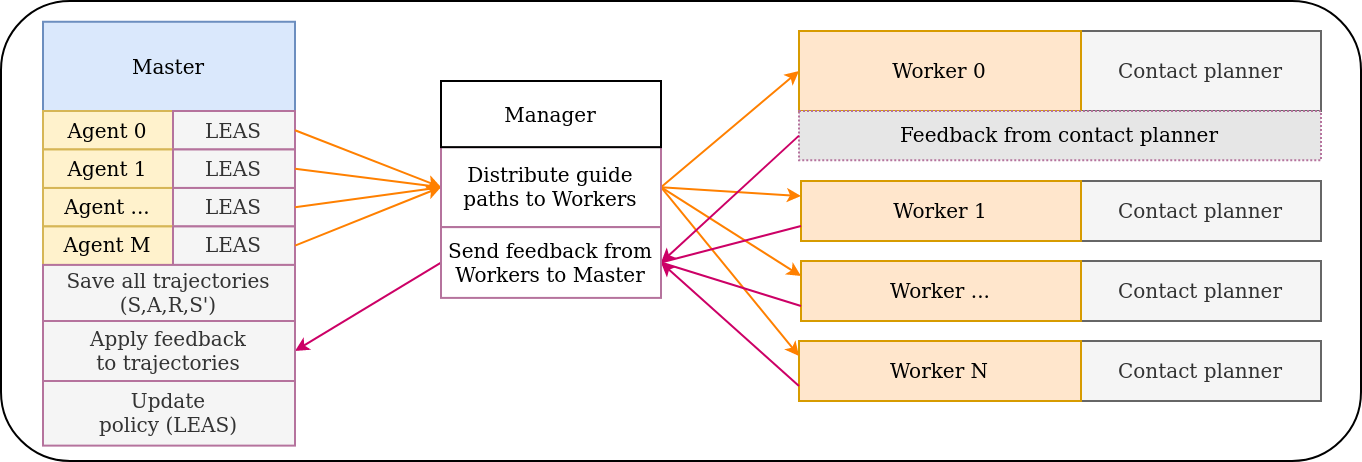
\includegraphics[width=\textwidth]{Figures/Chapter_LEAS/architecture_master_worker_1.png}
    \caption{Synchronous guide path and Asynchronous contact planning}
    \label{fig:architecture_master_worker_asynchronous}
    \end{subfigure}
    \caption{Two versions of Master-Workers architecture to learn LEAS plugged to a contact planner.}
    \label{fig:architecture_master_worker}
\end{figure}

% Solution A : all asynchronous
Solution (a) dissociates the learning operated by the master and the trajectory generation performed by the workers (so-called distributed RL).
The advantages of this method are its scalability, as we can add during the learning as many agents as desired that can run on different machines, and its modularity as the agents can be initialized on new terrain and stopped if needed.
This method is used in IMPALA \cite{impala2018} running 32 CPUs and RAPID \cite{openai2019dota} with 500 CPUs, showing impressive results to learn challenging and complex tasks.
However, this method also requires a lot of data exchanges between the RL algorithm and the workers as explained in \cite{evol_vs_rl_majid_2021}. 
The load on the network increases with the number of data (the trajectories) exchanged between the master and the workers, plus the parameters (policy network) that must be shared with all the workers after each update.
As a consequence, this approach can result in some hardware and implementation limitations depending on the available resources, and a possible delay in the policy of the asynchronous agents.

% Solution B : Guide path synchronous and contact planning asynchronous
The other solution (b) lets the master generate all the trajectories with one or several synchronous agents, then dispatch the guide paths generated to the workers that compute P2 and return the result to the master.
It is a solution specifically adapted to our problem and simple to implement that can be added on top of any on-policy or off-policy RL algorithm. 
%One or several agents generate synchronously some guide paths, that are shared with external workers that compute the contact sequence. Then, they return their feedback to the master for learning. 
The key advantage of this method is the reduction of data exchanges between the master and the workers. Only the guide path, a sequence of positions and orientations, and the feedback from the contact planner transit on the network.
However, if the guide path generation P1 is faster than P2, we can observe some lags between the synchronous agents and the workers. That is why we need to balance their number or add more workers to follow the flow. Also, the parallel agents during the learning run on environments that can not be changed manually, making it a simple but less modular method overall compared to (a).

In our experiments, solution (a) led to a bottleneck on our hardware due to the amount of data exchanged, and going for pre-made implementation as IMPALA was not necessary for our problem that only requires a few hours of training compared to the tasks solved in \cite{impala2018, openai2019dota}.
Therefore, we opted for solution (b) which is a good compromise between synchronous and asynchronous steps.
In the future, we would like to take a look at fully decentralized architectures \cite{DD_PPO} that solve the problem of network overload by sharing only the gradients for training.

With setup (b), we will now perform several tests on basic scenarios with LEAS without contact using the original PPO algorithm, then plug it into a contact planner using our modified PPO version to analyze its impact on the trained policy.

% Say that for the results bellow, we do not use the contact planners, equivalent to a contact planner that returns that all trajectories are succesful and returns last index of obs.

\section{Results\label{subsec:leas-results}}

\begin{table}[ht]
\begin{center}
\caption{Parameters}
\begin{tabular}{|c|c| c |c|c|}
 State & $81$ && Max Episode Length & $800$\\
 Actions & $4$ && Parallel agents & $6$\\
 $a_{max}$ & $0.08$ m/s$^2$ && Workers & $0$ \: or \: $6+$ \\
 $v_{max}$ & $0.2$ m/s && Batch size & $4096*M$\\
 $v_{desired}$ & $0.1$ m/s && Mini-Batch size & $256$\\
 $\omega_{max}$ & $\pi/9$ rad/s && Learning rate & $[5e-4,1e-5]$\\
 Timestep $T$ & $0.2$ s && Noptepochs & $10$\\
 Local height map $H$ & 10x14 && Discount Factor ($\gamma$) & $0.97$\\
 $z_{max}$ & $-0.2$ m  && Clip range & $0.2$\\
 $z_{min}$ & $-1.4$ m &&
 $w_{ori}$ & $0.4$ \\
 $w_{dir}$ & $1.0$  &&
 $w_{acc}$ & $0.1$ \\
 $w_{\omega}$ & $0.1$  &&
 $w_{alive}$ & $1.0$
\end{tabular}
\label{tab:param}
\end{center}
\end{table}

\begin{figure}
    \centering
    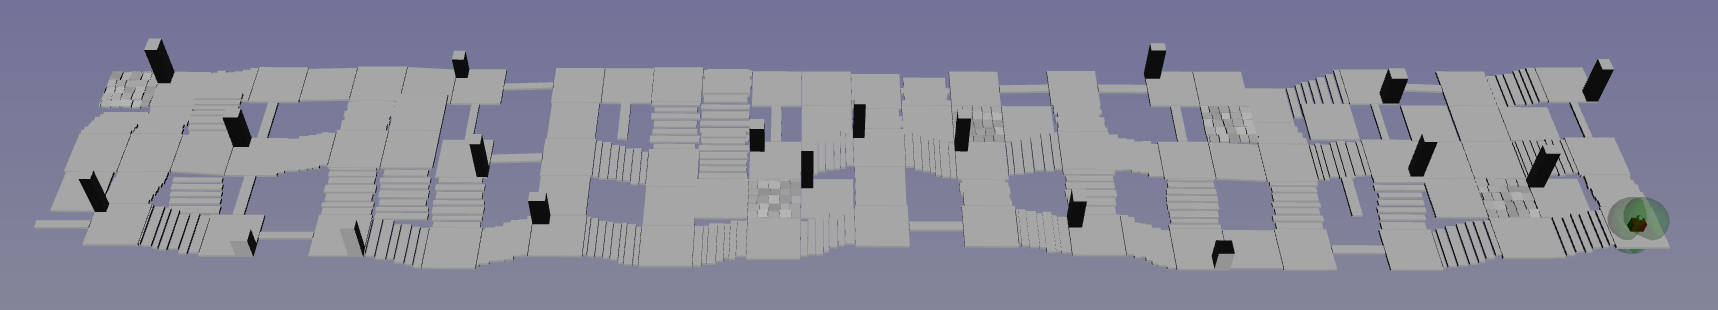
\includegraphics[width=\textwidth]{Figures/Chapter_LEAS/arena_5x30.png}
    \caption{Training ground of LEAS: a 5x30 arena (corresponding to 10x60 meters) composed of 86 links: 17 bridges, 31 stairs, 8 rubbles, and 30 flat ground with obstacles. All links are two-way and have different elements characteristics and slopes.}
    \label{fig:arena_5x30}
\end{figure}

% Explain what do we use
We use the HPP software \cite{HPP} and the humanoid robot Talos model \cite{talos_robot}. Our algorithm is implemented in python using the PPO implementation of Stable Baselines \cite{stable-baselines} modified for our Master-Workers architecture.
% Parameters
All parameters in the environment and hyperparameters to control the learning process can be seen in Table \ref{tab:param}. We use the terrain generator described in \ref{subsub:terrain_generator} to generate the 5x30 training ground in Figure \ref{fig:arena_5x30}.

% Explain parameters for the ENV
% - timestep => Why this value
We set a fixed timestep value $T =0.2$ seconds, which corresponds to a maximum distance between each state on the path of $4$ cm for $v_{max}=0.2$ m/s, and $2$ cm for $v_{desired}=0.1$ m/s.
% - number of steps max => Important to explore enough, not do only links and not be stuck somewhere.
Each episode has a maximum length of $800$ steps, meaning that the guide path can contain up to $800$ states (maximum distance of 32 meters). 
During the training, the robot has to navigate the terrain at the desired velocity while keeping a valid state ($\tilde{\mathcal{R}^*}$ and $\tilde{\mathcal{C}}$).
To further guide the learning, we initialize each episode as follows: first, the robot has to cross a link, i.e start from an initial tile and navigate through a transition tile (stairs, rubbles, or bridge), then, it has to follow a new random goal direction that is updated every $n_{rand} \in [200,800]$ steps.
The first goal prioritizes the task of crossing a link that we will perform in our basic scenarios, while the others often lead to a dead-end or a difficult path where the agent will have to learn if it has to stop or has the ability to cross it.

% Param for learning
We linearly decay the learning rate from $5e^-4$ to $1e-5$ over 2 millions training steps and set a discount factor $\gamma = 0.97$. 
A method to tune the discount factor is to calculate the half-life $\tau = \frac{1}{1-\gamma}$ which roughly corresponds to the number of steps considered to adapt the agent behavior. For LEAS, it is equal to $\tau = \frac{1}{1-0.97} \approx 33$ steps. 
As a result, steps from $[0,33]$, $[33,66]$, $[66,99]$, $[99,\infty]$ will roughly account for $63\%$, $23\%$, $8\%$ and $6\%$ of the sum of discounted rewards respectively. 
The distance traveled by the RL agent after 33 steps is equal to 66 cm and 132 cm for velocity equals to $v_{desired}$ and $v_{max}$ respectively.
% Notes: integral 0 to inf (0.97**x) = 32.8  => from 0 to 33=20.8 => from 33 to 66=7.6 => from 66 to 99 = 2.78. So most of the reward comes from 0 to 33 (64%), from 33 to 66 (23%), from 66 to 99=8%. If discount factor 0.98 : half-life at 50 => 0-50:64% => 50-100:23% => 100-150=8%
We emphasize that we want to learn a steering method to navigate locally and that the agent only needs to think about its very near future. For example the detection of an obstacle should impact its action only when close to the robot (distance inferior to 1 meter).

% Number of workers
In this chapter, the number of workers planning contacts is set to 0 as we train LEAS for a pure navigation task without a contact planner. In our experiment, the number of parallel agents is limited to 6 due to hardware limitations.

% Explain choices for the RL parameters used:
% - size of network with PPO : 256x128x64
The PPO actor and critic are two distinct networks with hidden layers of size 128x64x32. Tuning the number of nodes and hidden layers in the machine is empirical and depend on the task to perform. In general, deeper networks with more nodes means a better capability to solve very complex tasks and less under-fitting. However, it also means more parameters to train and can be prone to over-fitting. In our experiments on LEAS, we found no noticeable difference between 2 or 3 hidden layers and nodes number ranging from 64-256. However, we increased the network size of 64x64 from the first version of LEAS \cite{LEAS} for more potential scalability in our tests in terms of observations and contact planners.

We train LEAS without a contact planner and evaluate the model after 12 million steps corresponding to around 2 hour of training on a PC with an Intel Core i7-8700 (12 cores, 3.20Ghz, 16GB ram). Learning curves can be seen in figure \ref{fig:control_LEAS_learning_curves}.

\begin{figure}[ht]
    \centering
    %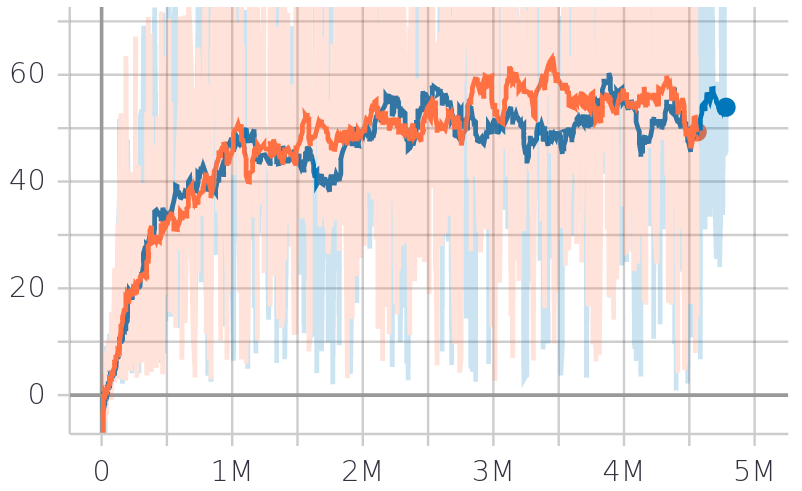
\includegraphics[width=0.6\textwidth]{Figures/Chapter_LEAS/learning_curves_P1.png}
    \begin{subfigure}[t]{0.49\linewidth}
    \includegraphics[width=\textwidth, height=4cm]{Figures/Chapter_LEAS/learning_curves_P1.png}
    \caption{}
    \end{subfigure}
    \begin{subfigure}[t]{0.49\linewidth}
    \includegraphics[width=\textwidth, height=4.5cm, trim={0cm 0.2cm 0cm 0cm},clip]{Figures/Chapter_LEAS/learning_curve_leas_p1.png}
    \caption{}
    \end{subfigure}
    \caption{Learning curves of LEAS without contact planner feedback (pure navigation task): (a) Comparison between an acceleration control (Orange) with delay, (Blue) without delay on the position update, and (b) the complete learning curve with an acceleration control.}
    \label{fig:control_LEAS_learning_curves}
\end{figure}


\subsection{Comparison: Steering Method Designs\label{tab:compare_sm_charac}}

\begin{table}[ht]
\caption{Comparison of the steering method characteristics.}
\begin{center}
\begin{tabular}{ |c|c|c|c| }
\hline
Steering Method & RB-Lin & RB-Kino & LEAS (ours)\\
\hline
Goal Connection & 
\thead{\textcolor{red}{Exact}\\pos,ori} & 
\thead{\textcolor{red}{Exact}\\pos,vel,acc,ori}  & 
\thead{\textcolor{blue}{Near}\\pos}
\\
\hline
Dynamic constraints &
\thead{\textcolor{red}{1}\\$v_{max}$} &
\thead{\textcolor{red}{2}\\$v_{max},a_{max}$} &
\thead{\textcolor{blue}{3}\\$v_{max},a_{max},\omega_{max}$}
\\
\hline
Terrain aware &
\thead{\textcolor{red}{No}} &
\thead{\textcolor{red}{No}} &
\thead{\textcolor{blue}{Yes}}
\\
\hline
\thead{Path planning\\dependant} &
\thead{\textcolor{red}{Yes}} &
\thead{\textcolor{red}{Yes}} &
\thead{\textcolor{blue}{No}}
\\
\hline
\end{tabular}
\end{center}
\end{table}

% Compare it to SM : RB-Kino and RB-Lin
% Show the difference between all SM :
% - RB-Kino connects exactly two points and its shape is relative to the two configs linked. 
% Advantage: connect exactly and we can control the acceleration and velocity at the goal + control on the acceleration.
% Disadvantage: Requires path planning to find the acc/vel/orientation at the arrival to obtain a valid guide path. Totally dependant on the path planning + can not be used for a control with a remote + does not consider the terrain to generate the trajectory.
% - RB-Lin connects exactly two points and do not perform DIMT, it's just a linear interpolation in velocity, orientation and position. No control on the acceleration.
% Advantage: Very simple to implement.
% Disadvantage: Also requires path planning as a line guide path is not sufficient very often to climb stairs + does not consider the terrain to generate the trajectory.
% - LEAS does not connect exactly two points and will just end up near the goal position.
% Advantage: Less dependant on path planning as the goal state is smaller (only position) and it can locally navigate depending on the terrain + control on the acceleration max.
% Disadvantage: No control on the velocity and orientation at the goal. Does not end exactly on the goal.
We compare LEAS, a flexible alternative to our previous steering methods. Their characteristics can be seen in Table \ref{tab:compare_sm_charac}.

\hfill

% Goal connection
\noindent \textbf{Goal connection}:
RB-Kino \cite{kinodynamic_sm_2017} and RB-Lin \cite{AcyclicCP} are two steering methods that connect exactly some initial and goal configurations in position, velocity, and orientation. 
% RB-Kino
RB-Kino uses the Double Integrator Minimum Time \cite{DIMT} to also add a constraint on the acceleration.
% LEAS
LEAS does not exactly connect the initial and goal configurations as it is trained to follow a given goal direction. Consequently, it can at best end up near the goal position.
The capability to connect exactly two configurations is needed in robotics for hand manipulation. Arguably, in locomotion, this accuracy is not required in most scenarios.
This is especially true on long paths with key waypoints to sequentially reach up to a distant objective, where passing close enough to each waypoint is sufficient.
As LEAS uses a target direction instead of a target configuration, it also enables us to use a joypad-like control, which is equivalent to a very distant moving target that the agent tries to reach. We simulate this kind of control for the training of LEAS by randomly repositioning its goal.

\hfill

% Dynamic constraints
\noindent \textbf{Dynamic constraints}:
% RB-Lin constraints
RB-Lin is a modified linear interpolation that is constrained in orientation and velocity. It first rotates the robot toward the target at $\omega_{max}$, then moves toward it at $v_{desired}$.
% RB-Kino constraints
RB-Kino requires two parameters $v_{max}$ and $a_{max}$ that act as strict constraints on both velocity and acceleration. However, no constraints are set on the angular velocity $\omega_{max}$ and this can be a problem as we will see in chapter \ref{sec:CP-SB}. 
%\textcolor{red}{TO CHECK, no constraint on angular velocity ? Why Pierre did not change it? He prefered starting with a higher init velocity to avoid this problem.}
% LEAS constraints
On the other hand, the control of LEAS constrains each configuration with $v_{max}$, $a_{max}$, $\omega_{max}$. 
In this thesis, we only use quasi-static contact planners, so $v_{max}$ and $a_{max}$ are considered during the guide path planning but not the contact planning phase. However, using LEAS with a kinodynamic contact planner is a possibility for future work.

\hfill

% Terrain aware + path planning
\noindent \textbf{Terrain-aware and path planning}:
RB-Kino and RB-Lin both require a path planning algorithm to place additional waypoints to reach a distant goal. In contrast, LEAS can observe its surrounding terrain and can locally navigate it in a given direction, hence removing the need for path planning on basic scenarios (i.e. crossing a link). 
In complex scenarios, path planning algorithms can also be used to place waypoints followed by LEAS. 
In this work, LEAS can navigate the same waypoints computed by the RRT with RB-Kino. In future work, having an RRT with LEAS in the same manner as RL-RRT \cite{RL_RRT} is a work in progress.

\hfill

Finally, we recall the main advantage of LEAS over our previous steering methods which is the use of Reinforcement Learning that, through the trajectory validation by the contact planner, can change its behavior to fit it and generate more likely feasible paths.

\subsection{Test Scenarios\label{subsub:leas:test_scenarios}}

As LEAS does not connect exactly with the goal position, we consider the goal to be reached when the distance from the current state on the guide path to the goal is lower than a distance threshold $\epsilon$ set to $20$ cm for all our scenarios.

% Show behaviour:
% [0] Navigate while keeping a desired velocity => Show acceleration, velocity, orientation, reward.
% Start from a -pi orientation.
% Show it on Ground.

% [2] On stairs, compare with RB-Kino/RB-Lin, the picture with the points, success SM.
\begin{figure}[ht]
    \centering
    \captionsetup[subfigure]{justification=centering}
    \begin{subfigure}[t]{0.49\linewidth}
    \centering
    \includegraphics[width=0.8\textwidth, height=5cm]{Figures/Chapter_LEAS/stairs_exemple.png}
    \caption{Scene view}
    \label{fig:stairs_p1:scene}
    \end{subfigure}
    \begin{subfigure}[t]{0.49\linewidth}
    \includegraphics[width=\textwidth, height=5cm,trim={2cm 2cm 2cm 2cm},clip]{Figures/Chapter_LEAS/stairs_lin_p1_90.png}
    \caption{RB-Lin}
    \label{fig:leas:stairs_p1_lin}
    \end{subfigure}
    \begin{subfigure}[t]{0.49\linewidth}
    \includegraphics[width=\textwidth, height=5cm,trim={2cm 2cm 2cm 2cm},clip]{Figures/Chapter_LEAS/stairs_kino_p1_90.png}
    \caption{RB-Kino}
    \label{fig:leas:stairs_p1_kino}
    \end{subfigure}
    \begin{subfigure}[t]{0.49\linewidth}
    \includegraphics[width=\textwidth, height=5cm,trim={2cm 2cm 2cm 2cm},clip]{Figures/Chapter_LEAS/stairs_leas_p1_90.png}
    \caption{LEAS (ours)}
    \label{fig:leas:stairs_p1_leas}
    \end{subfigure}
    \caption{Comparison on stairs where dots represent initial states from where the SM generates a valid (yellow) or invalid (black) guide path up to the goal (red). 
    The height map is represented by the grey shades from dark to bright, that are lower and higher heights respectively.
    We illustrate for each SM one trajectory where the black arrows represent the robot orientation along the guide.}
    \label{fig:stairs_p1}
\end{figure}

\hfill

\noindent\textbf{Stairs}. We compare the navigation skills of LEAS and our previous steering methods on the stairs scenario (Figure \ref{fig:stairs_p1}). 
%The height map of the terrain is represented by the grey shades with the bottom of the stairs on the left, and the top of the stairs on the right.
We uniformly sample 80 initial root configurations at the bottom of the stairs (Figure \ref{fig:stairs_p1:scene}), from which the steering methods have to generate guide paths up to the same fixed goal location.
Each initial state is oriented at $90^{\circ}$ with respect to the stairs, to better show the rotation performed by the steering methods, and with a null velocity. 
Initial states from where the SM reaches the goal with a valid guide path are represented by yellow dots. Conversely, black dots represent states where either the SM fails to reach the goal or generates an invalid guide path (i.e. ground not reachable or collision) and thus requires additional waypoints to be provided by a path planning method. 
For RB-Kino, we need to define some constraints that are the velocity and acceleration desired on the goal configuration and that have an impact on the shape of the trajectory. In this scenario, we set both goal acceleration and velocity to $0$.

RB-Lin is designed to first rotate the robot toward the goal, then generate a straight line up to the goal (Figure \ref{fig:leas:stairs_p1_lin}). Its main limitation is that it succeeds only when directly placed in front of the stairs, and further initial positions result in guide paths where the robot is unable to touch the ground.
RB-Kino presents the same limitation as RB-Lin, plus another one on the orientation where it rotates directly from $90^{\circ}$ to $0^{\circ}$ in one timestep (Figure \ref{fig:leas:stairs_p1_kino}). This is a problem inherent to RB-Kino which is the correlation between the initial velocity and the angular velocity. As a consequence starting with null velocity, as we will see later on, is critical with our contact planners as such fast rotation is not feasible kinematically. 
In practice, we avoid this problem by adopting the same strategy as RB-Lin by first rotating the robot to always start RB-Kino with a $0^{\circ}$ orientation.

LEAS  succeeds on a much broader range of initial states, hence removing the need for path planning in most cases (Figure \ref{fig:leas:stairs_p1_leas}). Our steering method generalizes to this scenario that has never been encountered during its training: it rotates and moves toward the goal, detects the stairs on its local height map, and adapts its velocity $v_z$ to climb it while keeping a valid state, finally reaching an area of $20$ cm around the goal.

% [2] On hole, compare with RB-Kino/RB-Lin, the picture with the points, success SM.
\hfill \break
\hfill \break

\begin{figure}[h]
    \centering
    \captionsetup[subfigure]{justification=centering}
    \begin{subfigure}[t]{0.4\linewidth}
    \includegraphics[width=\textwidth, height=4cm,trim={1cm 1cm 1cm 1cm},clip]{Figures/Chapter_LEAS/hole_p1_lin.png}
    \caption{RB-Lin}
    \label{fig:leas:hole:lin}
    \end{subfigure}
    \begin{subfigure}[t]{0.4\linewidth}
    \includegraphics[width=\textwidth, height=4cm,trim={1cm 1cm 1cm 1cm},clip]{Figures/Chapter_LEAS/hole_p1_kino.png}
    \caption{RB-Kino}
    \label{fig:leas:hole:kino}
    \end{subfigure}
    \begin{subfigure}[t]{0.4\linewidth}
    \includegraphics[width=\textwidth, height=4cm,trim={1cm 1cm 1cm 1cm},clip]{Figures/Chapter_LEAS/hole_p1_leas.png}
    \caption{LEAS (ours)}
    \label{fig:leas:hole:leas}
    \end{subfigure}
    \begin{subfigure}[t]{0.4\linewidth}
    \includegraphics[width=\textwidth, height=4cm,trim={1cm 1cm 1cm 1cm},clip]{Figures/Chapter_LEAS/hole_p1_kino_rrt.png}
    \caption{RB-Kino + RRT}
    \label{fig:leas:hole_scenarios_Kino_RRT}
    \label{fig:leas:hole:kino_rrt}
    \end{subfigure}
    \caption{Comparison of steering methods on hole scenario where dots are initial states from where the SM generates a valid (yellow) or invalid guide path (black) invalid guide path up to the goal (red). Guide paths are represented by the blue trajectories.}
    \label{fig:leas:hole_scenarios}
\end{figure}

\noindent\textbf{Hole}. We now compare our steering methods on our hole avoidance scenario (Figure \ref{fig:leas:hole_scenarios}). Each initial configuration has a null velocity and is oriented toward the goal located on the other side of the hole. 
RB-Kino and RB-Lin generate valid guide paths only when the problem is feasible in a straight line. It means that they require path planning for half of the initial configurations (Figures \ref{fig:leas:hole:lin} and \ref{fig:leas:hole:kino}).
In contrast, LEAS always succeeds in avoiding the hole and reaching the goal.
Even when starting from difficult configurations on the right, LEAS detects the hole and slowly slides along it while keeping a valid state.

% Still above the void
%We observe that some configurations still lie above the hole, less than 10 centimeters far from the surfaces. To fix this problem, a tighter constraint on the height map values under the robot can be set, as explained in Section \ref{subsub:validity_approximation}. %However, the Talos robot is 55 cm in width meaning that most of its body still lies above the ground.

%$\tilde{\mathcal{R}^*}$

% Hole kino and path planning
Finally, Figure \ref{fig:leas:hole_scenarios_Kino_RRT} illustrates RB-Kino combined with an RRT path planning algorithm to solve the hole scenario. The trajectories of (a,b,d) are generated using the full validity condition $\mathcal{R}$ without the stricter constraint (Section \ref{fig:approximation_validity}). Consequently, most guide paths generated lie above the hole with a maximum distance of $40$ cm from the surfaces, corresponding to the width of the range of motion of the Talos robot legs. 
This brings out the main problem of our previous validity condition $\mathcal{R}$ and the need to have a stricter constraint like $\tilde{\mathcal{R}^*}$ to avoid such configurations along the guide path.

%\textcolor{red}{TALK MORE ABOUT PATH PLANNING AND WHY WE DONT WANT TO USE IT HERE : 1.45s to compute it with bi-rrt on this scenario, several seconds on scenarios in their previous paper in C++. In comparison LEAS in python with my non-optimized code takes 0.56s in average on this scenario. => I can use the wall scenario to talk about that + need to add computation time on the hole scenario for Kino RRT}

% In general how much percent success in our scenarios ?
% -- On 1x11 with initial orientation of -180 degrees:
% Rubbles => 100/100
% Bridge => 31/100
% Stairs down => 100/100
% Stairs up => 86/100
% -- On 1x11 with initial orientation of 0 degrees:
% Rubbles => 100/100
% Bridge => 76/100
% Stairs down => 100/100
% Stairs up => 100/100

\hfill

\noindent\textbf{Evaluation of LEAS}. We evaluate the success of LEAS (Table \ref{tab:tests_1x11}) to navigate all the transition tiles of our evaluation terrain, never met during its training (Figure \ref{fig:tests_1x11}).
We uniformly sample 100 configurations before each transition tile with two different initial orientations, $0^{\circ}$ and $180^{\circ}$, to evaluate their impact on LEAS success. 


For both rubbles and stairs (down), LEAS succeeds in all 100 trajectories for both initial orientations.
Resuls show that our steering method succeeds in crossing all transition tiles of our scenario with a near $100$\% success rate, hence demonstrating its terrain-aware navigation skill.
%However, we observe some scenarios where our steering method fails
However, it also fails in some bridge and stairs (up) scenarios. This is mainly due to initial configurations facing backward and very close to the transition tile to cross. 
The agent thus fails to rotate the robot, to have a clear vision of the terrain in its back, before navigating it. 
These difficult cases appear on the bridge where the agent stops the robot near the void to avoid falling, and on the stairs up where the agent collides with it during its rotation.
%Despite these extreme cases, our steering method succeeds in crossing all the transition tiles of our scenario with a near $100$ \% success rate, hence demonstrating its terrain-aware navigation skills.
In pratice, the robot will never be positioned in such extreme initial configurations, hence the results show that our steering method can successfully navigate all our practical cases.


%Figure \ref{fig:leas_stop_void_obstacle} shows example scenarios where LEAS makes the robot idle to avoid unvalid configurations ($\mathcal{R}$ and $\mathcal{C}$).

%Finally, we manually place some waypoints to reach a distant goal on a complex scenario as seen in Figure \ref{fig:bauzil_waypoints}. LEAS successfully reaches each waypoint navigating across this terrain composed of stairs and a bridge.
Finally, we construct a scenario to sequentially cross different transition tiles (Figure \ref{fig:bauzil_waypoints}). To do so, we place manually chosen waypoints on the terrain to traverse some stairs and a bridge.
Results show that LEAS successfully reaches each waypoint, while generating valid configurations.

\begin{table}[h]
\centering
\begin{tabular}{ |c|c|c|c|c| } 
    \hline
    Initial orientation & Rubbles & Bridge & Stairs (down) & Stairs (up) \\ 
    \hline
    $0^{\circ}$ & 100 \% & 100 \% & 100 \% & 100 \%  \\ 
    \hline
    $180^{\circ}$ & 100 \% & 87 \% & 100 \% & 97 \% \\
    \hline
\end{tabular}
\caption{Success rate of LEAS For two initial orientations on 100 uniformly sampled trajectories for each transition tile (Figure \ref{fig:tests_1x11}). Initial positions can be far or near the transition tiles. LEAS needs enough time to rotate the robot, detect the transition tiles and navigate through it while keeping a valid configuration.}
\label{tab:tests_1x11}
\end{table}


\begin{figure}[h]
    \centering
    \includegraphics[width=0.8\textwidth,trim={0cm 0cm 0cm 0cm},clip, height=3cm]{Figures/Chapter_LEAS/1x11_tests.png}
    \includegraphics[width=\textwidth,trim={5cm 2cm 4cm 2cm},clip, height=5cm]{Figures/Chapter_LEAS/1x11_example_180deg.png}
    \caption{Evaluation terrrain with 4 transition tiles: rubbles, bridge, stairs (down), and stairs (up). Examples of extreme initial configurations (dots) from where LEAS generates: a valid (yellow) or invalid guide path (black) up to a goal (red). Black arrows are the root orientation along the guide (blue).}
    \label{fig:tests_1x11}
\end{figure}

% [1] Stop when there is an obstacle.
%\begin{figure}
%    \centering
%    \captionsetup[subfigure]{justification=centering}
%    \begin{subfigure}[t]{0.43\linewidth}
%    \includegraphics[width=\textwidth,height=6cm]{Figures/Chapter_LEAS/stop_bauzil_0.png}
%    \end{subfigure}
%    \begin{subfigure}[t]{0.43\linewidth}
%    \includegraphics[width=\textwidth,height=6cm]{Figures/Chapter_LEAS/stop_bauzil_1.png}
%    \end{subfigure}
%    \label{fig:leas_stop_void_obstacle}
%    \caption{LEAS detects an obstacle and lower its velocity to avoid any unvalid state: collision or ground not reachable (robot contact configurations computed with SB-CP for a better visualization).}
%\end{figure}

\begin{figure}[t]
    \centering
    \includegraphics[width=0.6\textwidth, height=5cm]{Figures/Chapter_LEAS/follow_waypoints_bauzil.png}
    \caption{LEAS connecting manually placed waypoints (yellow).}
    \label{fig:bauzil_waypoints}
\end{figure}




\section{Discussion\label{sub:leas:discussion}}
% Say that it works far better than before and offer a good compromise compared to our previous methods.
LEAS offers a flexible alternative to our previous steering methods. Our results show that LEAS performs better in generating valid guide paths, under collision-avoidance and reachability criteria, than RB-Kino and RB-Lin thanks to its local terrain awareness. 
This method learned by reinforcement succeeds in navigating all our test scenarios, while permitting a more flexible user control by providing a goal direction instead of a goal configuration. 
%However, it also presents some limitations in its design and further improvements will be required in the future.
However, there is still a lot of scope for improvements in its design.

\subsection{Limitations}
% FAILURE CASES
% Fail often on the bridge
\noindent\textbf{Terrain visualization}.
Parameters $[z_{min}, z_{max}]$ as well as the height map resolution impacts the agent capabilities to detect its environment.
In our experiments, the most difficult scenarios to handle were navigating through bridges and obstacle avoidance, where the tuning of these values was critical.
First, a too high value $z_{min}$ can lead LEAS to interpret the void surrounding the bridge as a potential stair.
This caused LEAS to lower the robot root, at the limit of the trunk collision with the bridge, to confirm if what it sees is a stair or a void. 
As a consequence, it can lead to some collisions with the bridge due to these two conflicting behaviors.
A similar problem appeared for a too low value $z_{max}$, with the interpretation of an obstacle as the next step of some stairs and causing a collision with it.
Finally, setting a too wide bound $[z_{min}, z_{max}]$ made the values of the heightmap difficult to interpret by our agent, that was unable to capture small to medium terrain variations.
The values we have selected offered a balanced trade-off, however, further tests are required to improve LEAS navigation performance.

% Play on R_ALIVE
To avoid such collisions, one could also increase $w_{alive}$ to encourage the robot to act more carefully. 
We tested this solution that greatly improved the LEAS capabilities for collision avoidance while keeping reachable states. However, LEAS was acting so safely that it did not dare to cross difficult transition tiles, sometimes making the robot idle in front of bridges to safely accumulate the reward $R_{alive}$. 
The final value $w_{alive}=1$ decided for LEAS offers a compromise safety/risk but requires further investigation. 

\hfill

% RL so the SM is not perfect and depends on many things
\noindent\textbf{Constraint on the orientation}. 
%Continuous agent learned by Reinforcement can still fail in performing their task, as LEAS due to a collision or staying idle instead of moving forward.
%An explanation of why the LEAS can present atypical behavior on some scenarios, why it does not succeed in generalizing or it generates guide path that are not straight is complex to analyze. It depends on the reward design, the control and the terrain where the agent has been trained on. 
% Exploration with orientation behaviour
We observed that LEAS trained on complex terrains tended to explore its surroundings by erratically orienting its root and so its local height map to have a better vision.
We limited this undesirable behavior by setting a high weight $w_{ori}$ to enforce its orientation toward the goal. 
However, such a reward will probably not work to navigate cluttered environments requiring the robot to sidewalk.

% Accuracy of LEAS
\begin{figure}
    \centering
    \includegraphics[width=0.6\textwidth, height=6cm]{Figures/Chapter_LEAS/test_epsilon.png}
    \caption{Average number of steps required to reach an area of radius $\epsilon$ cm around the goal.}
    \label{fig:nb_steps_required}
\end{figure}

\hfill

\noindent\textbf{Goal reaching accuracy}.
We recall one of the main limitations compared to our previous steering methods which is the non-exact connection to the goal position. We consider the goal as reached if the distance between the state on the guide path and the goal is inferior to a threshold of value $\epsilon$. In all our scenarios, we fix $\epsilon = 20$ cm that we consider accurate enough.
We further evaluate the accuracy of LEAS to reach a goal position in Figure \ref{fig:nb_steps_required}. For this test, we set the robot orientation back to the transition tile (rubbles for this scenario) and we uniformly sampled 50 configurations. The task to perform is to rotate the robot toward the fixed goal on the other side of the rubbles and get close to it, less than $\epsilon$ cm.
We test several values $\epsilon \in [1.5, 20]$ cm. 
For all $\epsilon \geq 1.5$ cm, all 50 trajectories reach the goal under the threshold. However, we can observe that as the value of epsilon decreases, the number of steps to reach the goal increases. Indeed, the agent passes close by the goal but misses the area of radius $\epsilon$ around it and has to move back and forth to reach such an accuracy. 
In this scenario, LEAS reaches the goal at once for all threshold $\geq 7.5 $ cm. In this thesis, we set $\epsilon=20$ cm to have a sufficient margin of error.

% Difficult to define good bounds for the height map to best represent small and high height variations. Using a second height map is a possibility but it increases the number of states and we want to avoid it. We could use a nonlinear, as a square function on values of the relative height map to better capture small variations near the robot's feet while ensuring height elevation detection for stairs, obstacles and void.
%\textbf{Surface detection}: 
\subsection{Future Improvements}

For a pure navigation task, LEAS without a contact planner does not need to clearly identify the surfaces of the terrain and solely focus on the reachability and collision conditions from the height map.
In this work we use a simple multilayer perceptron, as done in \cite{RL_RRT, RL_RRT_AUTORL} with 1-D lidar values, that is simple to implement and fast to train for our navigation task. 
However, we believe that LEAS could greatly benefit from convolutional neural network architectures to extract features from the height map and learn a better terrain representation \cite{deepLoco,deepGait,RLOC}.

The training terrain diversity was sufficient for LEAS to learn our navigation task, but more terrains could improve its generalization capabilities.
To do so, we could improve our terrain generator, or use another simulation environment such as RaiSim \cite{raisim} allowing us to efficiently switch between different terrains.

% How can we improve LEAS: As stated before, better terrains as grid terrains are still limited, biggers but with HPP not possible for now, more methods to have a better generalization with noise 
% + mirroring: it would be smart to mirror all the states and actions to generate twice as much datas. This would also get us a symmetric behaviour that we do not have for now.
%\textbf{Data augmentation}: 
Finally, we discussed using curriculum learning \cite{curriculum_learning_survey} to incrementally increase the complexity of the tasks to solve during the training, which did not improve the result of LEAS. But several methods in the literature could improve its learning efficiency and overall performance.
Especially mirroring all states relative to the robot orientation axis are other strategies to explore, that could greatly improve the sampling efficiency during the training and train a policy with a symmetric behavior.


\subsection{Conclusion}
% Recall that this is a prototype, but that is still better than our previous steering methods and in this paper we are aiming to see if a high level approach i.e. with a guide path can improve the performances of the contact planners.
% Conclusion
We presented LEAS, an RL steering method to locally navigate complex terrains and to generate guide paths subject to reachability and collision avoidance constraints. 
Such terrain-aware steering methods remove the need for a path planning algorithm, expensive to compute, in most of our basic scenarios.
As a result, LEAS can directly be integrated as the module P1 of our locomotion pipeline (Figure \ref{fig:pipeline}).

Yet, we did not solve the feasibility problem between our navigation task ($P1$) and the contact planner ($P2$), and that is why in the next chapters we answer the following question: 
\textit{can LEAS navigate complex terrains while generating feasible guide paths by a given contact planner?}


% ===========================================================================

\chapter{LEAS with an Acyclic Sampling Based Contact Planner}
\label{sec:CP-SB}
\minitoc
\bigskip

\begin{figure}[h]
    \centering
    \includegraphics[width=0.7\textwidth, height=5cm]{Figures/Chapter_CPSB/strategies_cp_guide_A.png}
    \caption{Given a guide path, our contact planner generates key configurations in contact along it.}
    \label{fig:cp-sb:strategy_cp-sb}
\end{figure}

% In this chapter, we present our first contact planner which populate the guide path with key configurations in double support contact
%\stn{Il faut faire tres attention ici. Faut commencer par dire que tu as besoin d un contact planner pour valider leas. C est delicat parce que ce st un chapitre entier de ta these qui est pas ta contrib, faut le dire direct}
%In this chapter we present the first contact planner we use in the module P2 of our multi-stage framework for locomotion: an acyclic Sampled-Based Contact Planner (SBCP) \cite{AcyclicCP} for multiped robot locomotion implemented in HPP software \stn{tu peux pas vraiment inventer des noms pour le travail des autres :D. Ou alors tu dis que tu utilises l acronyme pour simplifier} \cite{HPP_software}. We then explain \stn{???}

We have defined in the previous chapter a methodology to learn by reinforcement a local navigation method.
At evaluation time, our method LEAS produces a guide path along which we want to compute a contact sequence.

In a first phase, we used simple termination conditions during the training: the reachability $\tilde{\mathcal{R}^*}$ and the collision-free $\tilde{\mathcal{C}}$ conditions.
Yet those approximated conditions are necessary but not sufficient to guarantee the existence of a feasible contact sequence along the guide.

We now propose to explore the following question: \textit{What is a good guide path to generate a valid contact sequence ?}
For that, we will rely on an existing implementation of a contact planner, which we refer to as the second stage of our framework (P2). 
In this chapter, we use an acyclic Sample-Based Contact Planner \cite{AcyclicCP} for multiped robot locomotion, which for convenience we will refer to as SBCP.
As discussed in Chapter \ref{sec:LEAS}, we want LEAS to achieve two objectives:
\begin{itemize}
    \item Navigating using a local height map of the terrain toward a goal direction subject to some reachability and collision constraints;
    \item Generating guide paths (P1) maximizing the likelihood of finding feasible contact sequences along it with a contact planner (P2).
\end{itemize}
% What is the problem solved
In the context of Motion-before-Contact, LEAS learns to address by reinforcement one of the key limitations of this strategy: the non-guarantee of the feasibility of the guide (P1) by a contact planner (P2).

This chapter is organized as follows:
%section \ref{sub:cp-sb:implementation} we describe how the contact planner is implemented with the offline sampling of limb configurations, the contact generation and their solution to break down the combinatorics.
Section \ref{sub:cp-sb:implementation} is an overview of SBCP and its limitations due to the guide path. While this contact planner is not a contribution to this thesis, it is important to have a strong understanding of its structure and of the success and failure modes.
Section \ref{sub:cp-sb:leas_coupling} shows how to train LEAS with the contact planner as a black-box. 
Section \ref{sub:cp-sb:results} presents a benchmark and analysis of the results obtained by this contact planner with our steering methods.
Finally, section \ref{sub:cp-sb:discussion} discusses about our implementation choices and potential improvements to our work.


\section{Summary of the Sampling Based Contact Planner \label{sub:cp-sb:implementation}}

\subsection{Notations}

The Sample-Based Contact Planner (SBCP) \cite{AcyclicCP} belongs to the motion-before-contact family of contact planners, using a rough robot root trajectory (guide path) to generate the contacts along.
%In this work we do not use the arms of the robot and thus dismiss the multicontact aspect to focus on legged locomotion. \stn{la maniere plus simple de decrire le pb c est de parler de leas et de la validation et de dire naturellement que les scenarios etudies (que tu as deja definis precedemment) sont la marche bipedes}
While it can perform multi-contact locomotion tasks such as standing up or climbing stairs using a handrail, in this work we are interested in biped walking for the scenarios tested in Chapter \ref{sec:LEAS} where we only enable foot contacts with the terrain.
% Notations need to be consistant with part \ref{subsubsec:actions}

\newpage

We use the following syntax:
\begin{itemize}
    \item q$_{base}$ is the robot root configuration in SE$(3)$ (position and orientation);
    \item q$_k$ is the partial robot configuration on limb $k\in\{left\_leg, right\_leg\}$ with 6 degrees of freedom each. The methods allows a more generic multiped setup but we limited our benchmarks to biped cases;
    \item q $= [\mbox{q}_{base},\mbox{q}_{left\_leg},\mbox{q}_{right\_leg}]$ is the robot whole body configuration.
    \item G $ = [\mbox{q}_{base}^0,\mbox{q}_{base}^1,..., \mbox{q}_{base}^{M-1}]$ is the guide path, described as a sequence of M root configurations;
\end{itemize}

%We first explain how we sample the limb configuration of each joint and how we use it for contact creation, then we explain the contact planning process. \stn{pourquoi perdre du temps sur la base de donnees? On s en fout. Tu devrais expliquer le principe et finir en disant que pour gagner du temps on utilise une db. D abord expliquer le concept genereal}

% In this section we present an overview of SBCP, then we expose the feasibility problem with the guide path planner (P1).

\subsection{Overview of the Contact Planner}

%\textcolor{red}{I need to introduce N (samples), Robustness, MAX\_TRIES for repositioning}
\begin{figure}
    \centering
    \includegraphics[width=0.6\textwidth, height=5cm]{Figures/Chapter_CPSB/denoised_config_sampled.jpg}
    \caption{Sampling of limb configurations for the right leg of HRP-2 robot with (a) the leg range of motion and (b) some sampled configurations. Source: Tonneau et al. \cite{AcyclicCP}.}
    \label{fig:cp-sb:samples_rom}
\end{figure}

Given an initial whole body configuration $\mbox{q}^0$, the role of SBCP is to populate a guide path in input $G = [\mbox{q}_{base}^0,\mbox{q}_{base}^1,..., \mbox{q}_{base}^{M-1}]$ with a sequence of configurations in contact double support with the terrain and static equilibrium [$\mbox{q}^0$,$\mbox{q}^1$,..., $\mbox{q}^{M'-1}$] following \textbf{exactly} the guide path. 
% Comments steve
%\stn{le guide path il est continu en input, tu le discretises apres non ?} \textcolor{blue}{Non il est toujours discret.} 
%\stn{pourquoi L c est la config et pas q pour tout ? Sinon par convention en general les vecteurs c est minuscule gras, les grandes lettres c est pour les ensembles, ou en gras pour les matrices}

This is done in two steps: first, an offline sampling of limb configurations, second, an online search on these samples for the contacts to perform.

First, an offline database is generated containing configurations q$_k$ for each limb $k$. %to create contacts.
To do so, we randomly sample $N$ configurations for each limb inside their range of motion (Figure \ref{fig:cp-sb:samples_rom}).
This database will be searched at runtime, to select the most suitable limb configuration for a given root according to user-defined heuristics.
% and the measure of the $robustness$ of the equilibrium in the contact forces (More details about the measure of the robustness in \cite{AcyclicCP}). \textcolor{red}{I will use the measure of the robustness later, I don't know if I should explain it more or let it like this.}
We will discuss the heuristics used to search and select contact configurations, in particular the quantification of the robustness of the configuration balance, later in this chapter. %Section \ref{sub:cp-sb:leas_coupling}.

\begin{figure}
    \centering
    \includegraphics[width=\textwidth]{Figures/Chapter_CPSB/contact_maintain.png}
    \caption{Contacts are maintained on the next root position (green line) if kinematically feasible and without collision (2), they are broken otherwise (2,3). Source: Tonneau et al. \cite{AcyclicCP}.}
    \label{fig:overview_sbcp}
\end{figure}

% Role of the guide, SBCP follows exactly it and try to reach the next position on it.
Starting from a robot configuration $\mbox{q}^i$ in contact whose root is at q$_{base}^i$, the contact planner moves the robot root to the next position on the guide q$_{base}^{i+1}$. To do so, the contact planner performs the following steps (See figure \ref{fig:overview_sbcp}):
\begin{itemize}
    \item Maintain previous contacts: we check kinematically if the contact with the terrain on limb $k$ can be maintained from the next root position q$_{base}^{i+1}$. If not, the contact is broken.
    \item Repositioning: if more than one contact is broken in the previous step, one or more configurations in contact are added at q$_{base}^i$, to ensure that at most one contact is broken between $\mbox{q}^i$ and $\mbox{q}^{i+1}$. 
    %\stn{je pense qu on s en fout de ca} \textcolor{blue}{Il vaut mieux le dire quand meme non ? Surtout par rapport a MAX\_TRIES. Nicolas: c'est ok comme ca.}
    \item Creating contacts: if only one contact is broken, we create a new one with the limb $k$ that has been contact-free the longest. If the contact creation fails, we try to create contact with another free limb or reposition another limb in contact. If no contact can be computed to reach the next root configuration $\mbox{q}^{i+1}$ after a fixed number MAX\_TRIES of trials, SBCP returns the sub-sequence of successful configurations in contact up to $\mbox{q}^i$.
\end{itemize}
In this work, we focus on biped walking and so we perform contact only with the feet of the robot.
%, thus simplifying the algorithm. \stn{on dit pas que c est plus simple, ca simplifie pas l algo }
Obviously, setting a value of MAX\_TRIES $=2$ for the repositioning is sufficient for biped locomotion, where a higher threshold does not improve further its success but increases the computation time.
%Finally the sequence of configurations contains some limb configurations with redundant contacts position, i.e. where the position of the end-effectors are the same.  \stn{ca on s en fout}.
%That is why we only save the "key" configurations where a new contact is created and that we refer as the contact sequence outputed by SBCP. We refer the reader to \cite{AcyclicCP} for further details on the implementation of the contact planner.
% \stn{tu peux faire encore plus synthetique. t as une liste de config, une liste d effecteurs actif, et tu sors une liste de configurations en contact. Ensuite tu listes les raisons pour lesquelles ca va foirer, bonnes ou mauvaises. notamment si le guide est infaisable}
% Description of the complete pipeline RB-PRM (guide + SBCP)
Finally we recall the motion-before-contact strategy of SBCP in Figure \ref{fig:cp-sb:sbcp_explanation} with (a) generation of a guide path from an initial to a goal configuration respecting the reachability constraint $\tilde{\mathcal{R}^*}$ and collision-free $\tilde{\mathcal{C}}$, (b) creation of new contacts to sequentially reach each root configuration along the guide.
% What we said in chapter LEAS

\begin{figure}[h]
    \captionsetup[subfigure]{justification=centering}
    \centering
    \begin{subfigure}[t]{.48\linewidth}
    \includegraphics[width=\textwidth, height=4cm]{Figures/Chapter_CPSB/sbcp_explanation_0.png}
    \caption{}
    \end{subfigure}
    \begin{subfigure}[t]{.48\linewidth}
    \includegraphics[width=\textwidth, height=4cm]{Figures/Chapter_CPSB/sbcp_explanation_1.png}
    \caption{}
    \end{subfigure}
    \caption{Motion-before-contact strategy with SBCP: (a) generating a valid guide path and (b) computing the key configurations in contact along.}
    \label{fig:cp-sb:sbcp_explanation}
\end{figure}

\subsection{Limitation due to the Guide}

In Chapter \ref{sec:LEAS}, we have shown how LEAS generates guide paths subject to reachability and collision constraints ($\tilde{\mathcal{R}^*}$ and $\tilde{\mathcal{C}}$) for configuration validity. 

We now raise the key problem of the motion-before-contact strategy that is the non-guaranteed feasibility of the guide (P1) by the contact planner (P2).
% which hints us to some limitations of computing a contact sequence with SBCP using such guide paths.
%This limitation is encountered in many scenarios with our contact planner that can fail to compute a contact sequence following exactly a root trajectory.
% Our conclusion
Our experiments will show that the major factor impacting the contact planning success is the guide path in input.
% We do not know what is a "good" guide for SBCP, so it is difficult to approximate the feasibility using some manually designed heuristics. The reachability and collision conditions may not be sufficient
The problem is that we do not know what is a good guide path for this contact planner. 
The reachability and collision conditions introduced for configuration validity are necessary but not sufficient to generate guide paths feasible by this contact planner. 
%\textcolor{red}{Il faut que le sol soit atteignable et que la tronc ne soit pas en collision, sinon on ne peut pas faire de contact.}
As a consequence, it is difficult to define new additional constraints or heuristics to our guide path generator (P1) to better approximate the contact planning feasibility (P2).

Our solution to solve such a feasibility problem is to learn with LEAS how to validate its guide paths with SBCP, which computes the contact sequence along them. In other words, we want LEAS to answer the question: \textit{What is a feasible guide path for this contact planner ?}

%Finally, the resulting solution for the contact planning problem, LEAS plugged to SBCP, should be computationally efficient and present a better success rate than with our previous steering methods RB-Lin and RB-Kino on a wide range of scenarios.


% Problems more in details
%In our experiments, we found many cases where the guide paths even though valid (i.e. ground reachable and no collision along them) lead to a failure with SBCP on our test scenarios, thus motivating our search for a better steering method (P1).
%More specifically, we want to plug SBCP to LEAS to learn by reinforcement how to generate guide paths better fitting this contact planner.


\subsection{Trade-off in the Parameters \label{subsub:cp-sb:tradeoff}}
%\textcolor{blue}{Nicolas: Failure modes of the contact planner}

%We presented the overall concept of SBCP and the problem we are trying to solve in this section.
Before jumping onto our solution with LEAS, we identify two critical parameters whose tuning strongly impacts the success rate and the computation time of the contact planner:
\begin{itemize}
    \item $N$, the number of randomly sampled configurations q$_k$ for each limb $k$;
    \item $\Delta D$, the discretization step on the guide path, corresponding to the average distance between each root configuration q$_{base}^i$ to q$_{base}^{i+1}$ provided as input to the contact planner. 
    %\stn{tel que tu as ecrit les inputs ca arrive déjà discrétise...} \textcolor{blue}{C'est le cas.}
\end{itemize}
The first parameter $N$ is set offline, when initializing the database of limb configurations. The second parameter $\Delta D$ corresponds to the guide path discretization.
A trade-off has to be found on these values to comply with the requirements on the computation time and the success rate of the contact planner.
That is why we provide an analysis of both parameters and explain our choices for this work. The results are presented in Figure \ref{fig:cp-sb:impact_param_tuning}.

\begin{figure}[ht]
    \centering
    \captionsetup[subfigure]{justification=centering}
    \centering
    \begin{subfigure}[t]{.48\linewidth}
    \includegraphics[width=\textwidth, height=4cm,trim={0.5cm 0.5cm 0.5cm 0.5cm},clip]{Figures/Chapter_CPSB/success_time_samples.png}
    \caption{}
    \label{fig:cp-sb:impact_param_tuning:a}
    \end{subfigure}
    \begin{subfigure}[t]{.48\linewidth}
    \includegraphics[width=\textwidth, height=4cm,trim={0.5cm 0.5cm 0.5cm 0.5cm},clip]{Figures/Chapter_CPSB/success_time_discretization.png}
    \caption{}
    \label{fig:cp-sb:impact_param_tuning:b}
    \end{subfigure}
    \caption{Analysis of the success rate and computation time of SBCP with a guide path computed by RB-Kino in function of: (a) the number of samples $N$ and (b) the guide path discretization $\Delta D$ (average distance between the root configurations).}
    \label{fig:cp-sb:impact_param_tuning}
\end{figure}

\paragraph{Number of samples.}
The random sampling strategy consists in building a database of available configurations for each limb of the robot that is searched during the contact creation.
The number of samples $N$ is thus critical to provide enough coverage of the robot leg range of motion.
In this test, we measure the impact of the number of samples on the success rate and the computation time for complete successful guide paths only (Figure \ref{fig:cp-sb:impact_param_tuning:a}).
The success of a guide path is defined as the percentage of the successful guide with SBCP. For example, with a guide path of 100 configurations, if the contact planner fails to reach the configuration of index 50 then the success value is $50$\%.
% About the seed : it's complex, actually a seed with 25k samples work perfectly, but not with 50k...
We perform this test on the climbing stairs scenario (see Section \ref{sec:cp-sb:par:stairs}) where we generate some valid guide paths with RB-Kino from 100 uniformly sampled initial positions at the bottom of the stairs oriented toward the goal. 
We then evaluate the results of different sample values $N$ for 3 different seeds, with an average guide path discretization step $\Delta D = 2$cm. 
We will explain the choice of $\Delta D$ later on in this section.

We observe that (red) the success rate rapidly converges to a maximum success rate on this task, and that (blue) the contact planning time increases with the number of samples $N$.
From these results, we can deduce that a number of samples $N=10K$ is sufficient to solve this particular locomotion task.
However, reducing the value of this parameter beyond a certain point increases the computation time, where the contact planner requires contact repositioning to compensate for the lack of sampled configurations leading to a robust solution.
As a result, we found the sweet spot to be $N=25K$ for the stairs and that we keep fixed in our setting across our scenarios. 
It is unsure how this small number of samples copes with more complex terrains like our 5x30 training ground, but we can expect a lower feasibility space with SCBP and where the guide path quality becomes more important.


\paragraph{Guide path discretization.}
The discretization step $\Delta D$ on the guide path corresponds to the average distance between each root configuration q$_{base}^i$ to q$_{base}^{i+1}$. A small $\Delta D$ means a higher number of root configurations on the guide, that results in a higher number of footsteps with SBCP. 
A small value increases its success rate but also its computation time as observed in Figure \ref{fig:cp-sb:impact_param_tuning:b}.
% How is the test done
This test is performed on the same stairs scenario with the steering method RB-Kino. 
RB-Kino generates guide paths continuous in time with non-constant velocities that
we discretize with a fixed timestep. 
We sample some timestep values and measure the corresponding average velocity on the guide, and thus its discretization step $\Delta D$.
We compute 50 trajectories for each measurement and average the results over 3 different seeds and three sample numbers, $N=\{25,50,100\}$K. 

% Comparison with discretization of the guide in acyclic
We compare these results to the original paper \cite{AcyclicCP} using the robot HRP-2 that has a similar maximum step size to the robot Talos we work on. They state that "in most scenarios the torso of HRP-2 moves about 15 cm (for easy scenarios) between two postures, but only 3 cm for the car egress scenario". 
% Results
From our measurements, we see that a small discretization step $\Delta D=2$ cm on the guide increases the success rate of the contact planner. 
Indeed, it is easier for the robot to create a contact to reach a closer root configuration than a distant one.
%However, a small discretization step also comes at the cost of a higher computation time as SBCP generates more configurations in contact along the guide.
% Find a trade-off
The choice of $\Delta D$ is a trade-off between the success rate and the number of steps (and so the computation time). 
One could just set an average discretization $\Delta D=2$ cm that could maximize the success rate in most scenarios. However, this also results in a high contact planning time (over a second) and a hundred footsteps for a trajectory of $3$ to $4$ meters for the climbing stairs task, which is not tolerable.
In this work, we aim for an average discretization $\Delta D=10$ cm resulting in a satisfactory number of steps and computation time, while providing a sufficient success rate on SBCP with our previous steering methods. 
Just as the tuning of the parameter $N$, such a high value of $\Delta D$ lowers the success rate of the guide with SBCP, and so greater emphasizes the quality of the guide (i.e. the positioning of the root configurations relative to the terrain).
On all our steering methods, we further discretize the guide when required to obtain an average $\Delta D=10$ cm and thus provide a fairer comparison with closely matched settings.

\hfill

% Conclusion
% We said all the possibilities in hpp, say the one that is actually chosen in most of their scenario and what could have been nice to work on.
%We presented the general concept behind our sample-based contact planner (P2) computing a contact sequence following exactly the guide in input (P1). We then presented some parameters to analyze the critical part of such contact planning strategy and conclude it to be the input guide path, that is the focus of our research.
We presented the general concept behind our sample-based contact planner (P2) computing a contact sequence following exactly the guide path in input (P1), and our design choice for two critical parameters.
% Modif of nicolas
As we have seen, it is important to design the guide path to have good properties with respect to the contact planner. 
However, these properties are difficult to express explicitly, making it difficult to build heuristics or a more optimal decision process for computing the guide path. 
We then propose to formulate it as a maximization of the success likelihood of the contact planner, building upon LEAS for the learning algorithm. Let's now see the details of this proposition.

% ========================================================================

\section{Implementation Details\label{sub:cp-sb:leas_coupling}}
% Explain the motivation and clearly state what we want to do and hope.
%Our sample-based contact planner presents several limitations due to the separation with the guide path planner P1. We observe on our previous steering methods RB-Lin and RB-Kino plugged to SBCP a drop in the success rate of the contact planning, highlighting the difficulty to design efficient but general enough heuristics that works well on most problems.

Our goal with our steering method LEAS is to overcome the challenges coming from the connection of the guide path planner and the contact planner with a high-level approach.
We want to generate guide paths that are feasible by the contact planner.

% - it implements a stricter constraint to approximate the contact reachable space, further increasing the probability to have more sampled configurations in contact with the terrain.
In the previous chapter, we have shown how LEAS performs in a navigation task with its local terrain-aware capability.
In simple scenarios, LEAS does not heavily rely on path planning algorithms compared to our previous steering methods, resulting in an overall faster generation of guide paths.
%\stn{il faut que tu remplaces tous tes efficient par des termes precis. En quoi elle est mieux que quoi ? sur quelle metrique?}
We now want to improve the feasibility of the generated guide paths by our sample-based contact planner.
% - RL with the SBCP as a black-box, introduce a synergy between P1 and P2 and attempt to alleviate the previously cited limitations intrinsic and extrinsic of SBCP.
We employ the strategy described in the previous chapter with our Master-Workers architecture where the workers validate the trajectories generated by the LEAS agents, by computing the contact sequence along the guides with SBCP used as a black box.
%To do so, we plug SBCP (P2) as a black-box, that computes the contact sequence along the guides generated by LEAS and feedbacks a validation of it during the learning.

\subsection{Parameters of LEAS with Contact Planner}
% - Implementation detail
% - Network
\paragraph{RL policy.}
We employ the same network architecture, states, actions, rewards, and hyperparameters as described in Chapter \ref{sec:LEAS} and set the number of asynchronous workers computing the contacts to 6.
Our method LEAS takes as input a local height map of the terrain and a direction to the goal to locally navigate the terrain. 
States generated by LEAS are subject to the reachability $\tilde{\mathcal{R}^*}$ and collision-free $\tilde{\mathcal{C}}$ conditions, plus a new additional constraint on the whole guide path that is to succeed with the contact planner, that we will explain later on.

% About the CP param
\paragraph{Contact planner parameters.}
We authorize the contact with the limbs $k=$ \{$left\_leg$, $right\_leg$\} to perform a biped locomotion task only, and generate for each limb a number of samples $N=25$K with a fixed seed (empirically selected). Finally, the number of maximum repositioning attempts in the contact planner is set to MAX\_TRIES $=2$, sufficient for our biped locomotion task.

% About the guide / LEAS
% Originally in LEAS
\paragraph{Guide path discretization.}
The discretization of the guide generated by LEAS corresponds to an average of $\Delta D=2$cm between each configuration. 
As seen in the previous section, this value presents on SBCP the best success rate at the cost of a very high computation time, as it generates contact plans with too many contacts (over a hundred steps to walk 3 to 4 meters).
% What we do
That is why we want to aim for an average $\Delta D=10$cm, presenting a suitable trade-off in computation time and success rate with this contact planner.
To do so, we further discretize the guide path before giving it to the contact planner by only keeping 1 out of 5 root configurations on it, to aim for a discretization step of $\Delta D = 2 \times 5 = 10$cm in average (further discussed in section \ref{sub:cp-sb:discussion}).



\subsection{Validation by the Contact Planner}
\begin{figure}[ht]
    \captionsetup[subfigure]{justification=centering}
    \centering
    \begin{subfigure}[t]{.35\linewidth}
    \includegraphics[width=\textwidth, height=4cm]{Figures/Chapter_CPSB/example_fail_planning.png}
    \caption{}
    \end{subfigure}
    \begin{subfigure}[t]{.60\linewidth}
    \includegraphics[width=\textwidth, height=4cm]{Figures/Chapter_CPSB/example_fail_planning_diagram.png}
    \caption{}
    \end{subfigure}
    \caption{Generation of a guide path that fails with SBCP: (a) generation of a valid guide path up to configuration 5 and fail of the contact planner at 3, (b) diagram of the learning process from this trajectory.}
    \label{fig:cp-sb:remove_fail_path}
\end{figure}
% What will happen ?
During the learning, the workers perform contact planning with SBCP to validate the trajectories generated by LEAS. Therefore, it learns how to generate feasible guide paths according to the validity conditions $\tilde{\mathcal{R}^*}$ and $\tilde{\mathcal{C}}$, plus the contact planner (P2).
% What is the validation by SBCP
Our contact planner returns the contact sequence along the guide, up to the last successful root configuration q$_{base}^i$.
The index of this configuration is retrieved and sent back to the master that prunes the section of the guide path that failed as depicted in Figure \ref{fig:cp-sb:remove_fail_path}.
% - to learn how to improve the CP-SB success rate => How do we do ? Propagation of the result of CP-SB on the trajectory generated by LEAS.
LEAS has to find a trade-off between learning the navigation task presented in Chapter \ref{sec:LEAS} and succeeding in the contact planning.

\subsection{Training}
\begin{figure}[t]
    \centering
    \includegraphics[width=0.6\textwidth]{Figures/Chapter_CPSB/learning_curve_p1_p2.png}
    \caption{Learning curves of (blue) LEAS-P1 trained without contact planner and (red) LEAS-P2 trained with guide validation by SBCP.}
    \label{fig:cp-sb:learning_curves_p1_p2}
\end{figure}
We train LEAS with SBCP on our training terrain presented in the previous chapter.
The model is evaluated after 12 million steps corresponding to 8 hours of training on a PC with an Intel Core i7-8700 (12 cores, 3.20Ghz, 16GB ram). 
Learning curves of LEAS without a contact planner, referred to as LEAS-P1 (Chapter \ref{sec:LEAS}), and LEAS with the contact planner, LEAS-P2, are shown in Figure \ref{fig:cp-sb:learning_curves_p1_p2} (the maximum reward is equal to 100 for trajectories in a straight line at $v_{desired}$). 
The P2 validation increases its probability to meet a terminal condition (i.e. failing the contact planning) and forces LEAS to adapt its behavior to succeed with the contact planner, hence resulting in a lower average reward per episode.

\section{Results\label{sub:cp-sb:results}}

%\paragraph{Evaluation methodology}
For all our tests, we uniformly sample some initial configurations on a flat area and set a fixed goal configuration on the other side of the obstacle to cross, corresponding to trajectories of 3 to 4 meters long in average.
Each steering method has to generate guide paths with valid configurations ($\tilde{\mathcal{R}^*}$ and $\tilde{\mathcal{C}}$) up to the target and compute a contact sequence along it with SBCP.
The success rate presented in the results corresponds to the percentage of valid guide paths reaching the goal and being successful with SBCP.
% Tuning of discretization step
We tune the discretization timestep of RB-Kino and RB-Lin such that the discretization step along the guide is on average equal to $\Delta D=10$cm, just as LEAS.
% Comments
%\stn{comment t usais que c est "fair". Es tu certain qu un pas discret est tjs synonyme de meilleur succes? }

We compare the method proposed in this chapter (LEAS-P2), with the method proposed in the previous chapter (LEAS-P1) and the two model-based steering methods used as benchmarks, RB-Lin and RB-Kino. We evaluate them on scenarios we know, from experience, to be challenging for contact planners. For each scenario, we analyze the changes in the guide path generation, hinting us about our contact planner capability relative to the guide.

\subsection{Scenario A: Rotation\label{subsub:sbcp:rotation}}
Given initial and target configurations, we uniformly sample some initial robot orientations and set some fixed velocity values to evaluate the success of all steering methods with the contact planner. The orientation value corresponds to the angle between the target direction and the root orientation. 
We evaluate the success rate of each steering method that has to rotate and move the robot to the goal. 
This scenario simulates a problem that some heuristic methods cannot solve well. While these methods could be specifically patched to counteract it, it is interesting to understand these behaviors.

In this experiment, all steering methods succeed in generating a valid guide path, reachable and without collision, up to the target but present different results as seen in Table \ref{tab:cp-sb:rotation_success} and Figure \ref{fig:cp-sb:rotation_scenario}. 

\begin{table}[ht]
\centering
\caption{Scenario A: success rate for different orientations on flat ground.\label{tab:SBCP:ground_ori}}
\begin{tabular}{ |c|c|c|c|c| }
    \hline
    \makecell{Parameters} & \makecell{RB-Lin} & RB-Kino & LEAS-P1 & LEAS-P2\\
    \hline
    $0^{\circ}$ to $30^{\circ}$ &  & & & \\
    $||v||$ = 0 & 100\% & 100\% & 100\% & 100\% \\
    $||v||$ = 0.04 & x & 100\% & 100\% & 100\% \\
    $||v||$ = 0.07 & x & 100\% & 100\% & 100\% \\
    \hline
    $60^{\circ}$ to $120^{\circ}$ &  & & & \\
    $||v||$ = 0 & 100\% & 61 \% & 75\% & 100\% \\
    $||v||$ = 0.04 & x & 100\% & 84\% & 100\% \\
    $||v||$ = 0.07 & x & 100\% & 89\% & 100\% \\
    \hline
    $150^{\circ}$ to $180^{\circ}$ &  & & & \\
    $||v||$ = 0 & 100 \% & 0 \% & 22 \% &  100\% \\
    $||v||$ = 0.04 & x & 0 \% & 35 \% & 100\% \\
    $||v||$ = 0.07 & x & 43 \% & 42 \% & 100\% \\
    \hline
\end{tabular}
\label{tab:cp-sb:rotation_success}
\end{table}
\begin{figure}[ht]
    \captionsetup[subfigure]{justification=centering}
    \centering
    \begin{subfigure}[t]{0.49\linewidth}
    \includegraphics[width=\textwidth]{Figures/Chapter_CPSB/rotation_lin_180_v04.png}
    \caption{RB-Lin}
    \end{subfigure}
    \begin{subfigure}[t]{0.49\linewidth}
    \includegraphics[width=\textwidth]{Figures/Chapter_CPSB/rotation_kino_180_v04.png}
    \caption{RB-Kino}
    \end{subfigure}
    \begin{subfigure}[t]{0.49\linewidth}
    \includegraphics[width=\textwidth]{Figures/Chapter_CPSB/rotation_p1_180_v04.png}
    \caption{LEAS-P1}
    \label{fig:cp-sb:rotation_scenario:leas_p1}
    \end{subfigure}
    \begin{subfigure}[t]{0.49\linewidth}
    \includegraphics[width=\textwidth]{Figures/Chapter_CPSB/rotation_p2_180_v04.png}
    \caption{LEAS-P2}
    \label{fig:cp-sb:rotation_scenario:leas_p2}
    \end{subfigure}
    \caption{Scenario A, Trajectories for initial configurations at $180^{\circ}$ and $||v||=0.04$ m/s with (blue) the successful and (yellow) the failed part of the guide, and (black arrow) the robot root orientation.}
    \label{fig:cp-sb:rotation_scenario}
\end{figure}
\begin{figure}[ht]
    \captionsetup[subfigure]{justification=centering}
    \centering
    \includegraphics[trim={2cm 2cm 4cm 2cm}, clip,width=0.32\textwidth]{Figures/Chapter_CPSB/rotation_seq/rot2.png}
    \includegraphics[trim={2cm 2cm 4cm 2cm}, clip,width=0.32\textwidth]{Figures/Chapter_CPSB/rotation_seq/rot3.png}
    \includegraphics[trim={2cm 2cm 4cm 2cm}, clip,width=0.32\textwidth]{Figures/Chapter_CPSB/rotation_seq/rot4.png}
    \caption{Scenario A: Sequence of configurations where LEAS-P1 fails the rotation along the guide.}
    \label{fig:cp-sb:rotation_leas_p1_fail}
\end{figure}

% RB-Lin results => Work all the time with $\omega_{max}$, it's like a sanity test.
RB-Lin rotates at a fixed angular velocity $\omega_{max}=\frac{\pi}{9}=20$ deg/s which is equal for $T=0.2$ s to a maximum rotation of $\omega_{max} \times T \times 5 = 20^{\circ}$ between each configurations on the guide (keeping 1 out 5 guide configurations).
As expected, the results show that for any initial orientation, rotating the robot with a step angle of $20^{\circ}$ before moving it to the goal generates feasible guide paths by the contact planner. 
RB-Lin shows that a rotation toward the goal, with a step angle $20^{\circ}$ between the guide path configurations, can safely be performed before moving the robot. 
In our tests, all step angles in the range $]0,90]$ degrees were successful, but in practice, a step angle of $45^{\circ}$ may be the maximum feasible by the Talos robot in reality.

RB-Kino succeeds for all orientations in $[0,120]$ degrees. 
However, we can see the limitation of RB-Kino when starting with a (near) null velocity as discussed in the previous chapter, and as a result, fails the contact planning as such high rotation is not kinematically feasible. 
We recall that in practice we adopt the same strategy that RB-Lin by rotating the robot first before using RB-Kino, and thus we always avoid such cases.
% Comments steve
%\stn{on avait dit qu on en parlait pas ? c est un bug facilement contournable, tu devrais mettre 100 la} 
%\textcolor{blue}{Dans ce cas la, ce test sur la rotation ne sert a rien non ? Vu qu'on va toujours tourner le robot vers l'objectif avant de le faire bouger et on aura 100\% de succes partout. J'explique bien apres qu'en general avec RB-Kino on ne va jamais se retrouver dans ce cas la. Nicolas: Il a barré cette discussion donc je suppose que ca veut dire ok.}

Then we compare LEAS-P1 and LEAS-P2 that have been trained with and without feedback from the contact planner respectively.
% What these two agents share in common and do not.
LEAS-P1 is subject to two major rewards motivating its behavior: $R_{ori}$, encouraging him to be oriented to the target and $R_{dir}$ to move toward it at $v_{desired}$. 
As a result, LEAS-P1 balances these two rewards by moving and rotating at the same time. 
Additionally, LEAS-P2 is subject to another constraint that is to succeed with the contact planner (P2).

% Results of LEAS-P1
The results show that LEAS-P1 works for all initial orientations in $[0,30]$ degrees but may fail for initial orientations superior to $60^{\circ}$.
%It is interesting to note that LEAS has its angular velocity $\omega < \omega_{max}$ but fails some rotations compared to RB-Lin. 
Indeed, rotating while moving toward the target is more difficult and requires adapting simultaneously the robot velocity and angular velocity.
Finally, as the initial velocity increases, we can note that so does the success rate with LEAS-P1 and RB-Kino.

% Results of LEAS-P2
In contrast, LEAS-P2 learns how to rotate and succeeds in every rotation scenarios, thus showing the benefit of our solution.
% Analyze how LEAS-P2 rotates better than LEAS-P1 => Visually + how it sacrifices the reward (no sacrifice for this scenario) ?
%However it is difficult to evaluate why LEAS-P2 presents a better success rate than LEAS-P1 (Figure \ref{fig:cp-sb:rotation_scenario}). 
Empirically, we noticed that LEAS-P2 tends to move in the direction of its orientation to help the rotation task (Figure \ref{fig:cp-sb:rotation_scenario:leas_p2}), whereas backward translations with LEAS-P1 could result in failure due to heuristics defined in the contact planner (Figure \ref{fig:cp-sb:rotation_scenario:leas_p1}).
That is why some guide paths generated by LEAS-P1 leads to some configurations that do not permit further movement (Figure \ref{fig:cp-sb:rotation_leas_p1_fail}). 
In contrast, LEAS-P2 automatically discovers how to generate guide paths avoiding the selection of such configurations from the samples.


\subsection{Scenarios B: Obstacle Avoidance}
% Use the hole and bridge from 1x11.
% Hole and bridge are quite similar because when the SM succeeds, it often passes very close to the edge and should avoid it to succeed SBCP.
\begin{figure}[t]
    \captionsetup[subfigure]{justification=centering}
    \centering
    \begin{subfigure}[t]{0.48\linewidth}
        \includegraphics[width=\textwidth, height=6cm]{Figures/Chapter_CPSB/hole_scenario.png}
    \end{subfigure}
    \begin{subfigure}[t]{0.48\linewidth}
        \includegraphics[width=\textwidth, height=6cm]{Figures/Chapter_CPSB/bridge_scenario.png}
    \end{subfigure}
    \caption{Scenario B1: The steering method has to generate a valid guide path (yellow) up to the goal (red), then compute a contact sequence along it with SBCP.}
    \label{fig:cp-sb:scenarios_hole_bridge}
\end{figure}

\begin{table}[h]
\centering
\caption{Scenario B1: Comparison on the success rate and robustness.}
\begin{tabular}{ |c|c|c|c|c|c| }
    \hline
    Parameters & Terrains & RB-Lin & RB-Kino & LEAS-P1 & LEAS-P2\\
    \hline \hline
    \multirow{3}{*}{SR} & Hole & 82\% & 74\% & 100\% & 100\% \\
    \cline{2-6}
                        & Bridge & 86\% & 78\% & 96\% & 100\% \\
    \hline \hline
    \multirow{3}{*}{Robustness} & Hole & 21.7 & 20.9 & 32.2 & 33.3 \\
    \cline{2-6}
                        & Bridge & 20.84 & 25.8 & 24.36 & 27.3 \\
    \hline
\end{tabular}
\label{tab:cp-sb:hole_bridge}
\end{table}

\begin{figure}[ht]
    \captionsetup[subfigure]{justification=centering}
    \centering
    \begin{subfigure}[t]{0.4\linewidth}
        \includegraphics[width=\textwidth, height=3.5cm, trim={0cm 1cm 0cm 1cm},clip]{Figures/Chapter_CPSB/hole_Lin.png}
        \caption{RB-Lin}
    \end{subfigure}
    \begin{subfigure}[t]{0.4\linewidth}
        \includegraphics[width=\textwidth, height=3.5cm, trim={0cm 1cm 0cm 1cm},clip]{Figures/Chapter_CPSB/hole_Kino.png}
        \caption{RB-Kino}
    \end{subfigure}
    \begin{subfigure}[t]{0.4\linewidth}
        \includegraphics[width=\textwidth, height=3.5cm, trim={0cm 1cm 0cm 1cm},clip]{Figures/Chapter_CPSB/hole_LEAS-P1.png}
        \caption{LEAS-P1}
    \end{subfigure}
    \begin{subfigure}[t]{0.4\linewidth}
        \includegraphics[width=\textwidth, height=3.5cm, trim={0cm 1cm 0cm 1cm},clip]{Figures/Chapter_CPSB/hole_LEAS-P2.png}
        \caption{LEAS-P2}
    \end{subfigure}
    \caption{Scenario B1 (hole): initial configurations succeeding (yellow dot) and failing (magenta dot) with SBCP.}
    \label{fig:cp-sb:trajectories_hole}
\end{figure}


\begin{figure}[h!]
    \captionsetup[subfigure]{justification=centering}
    \centering
    \begin{subfigure}[t]{0.32\linewidth}
        \includegraphics[width=\textwidth, height=5cm]{Figures/Chapter_CPSB/talos_bridge_kino.png}
        \caption{}
        \label{fig:cp-sb:talos_configurations_hole_bridge_block0}
    \end{subfigure}
    \begin{subfigure}[t]{0.32\linewidth}
        \includegraphics[width=\textwidth, height=5cm]{Figures/Chapter_CPSB/talos_hole_kino.png}
        \caption{}
        \label{fig:cp-sb:talos_configurations_hole_bridge_block1}
    \end{subfigure}
    \begin{subfigure}[t]{0.32\linewidth}
        \includegraphics[width=\textwidth, height=5cm]{Figures/Chapter_CPSB/talos_hole_not_good.png}
        \caption{}
        \label{fig:cp-sb:talos_configurations_hole_bridge_unfeasible}
    \end{subfigure}
    \caption{Scenario B1: (a)(b) blocking Talos configurations above the void  and (c) configuration valid but unfeasible on the real robot.}
    \label{fig:cp-sb:talos_configurations_hole_bridge}
\end{figure}


% What is tested
\paragraph{Scenario B1 - Hole and Bridge.} 
We compute contact sequences on guide paths generated by our steering methods on the hole and bridge scenarios (Figure \ref{fig:cp-sb:scenarios_hole_bridge}). 
These two scenarios are similar as they can both lead to weak contact configurations located very close to the edge of the obstacles that are unfeasible by the robot in reality (Figure \ref{fig:cp-sb:talos_configurations_hole_bridge}).
We evaluate for both terrains the success rate with the contact planner and measure the average $robustness$ of the configurations in contact when passing near the obstacle.
% What is the robustness used for
The robustness quantifies how far the center of mass of the robot is from the boundaries of the friction cones of the contact forces, giving us a measure of the static equilibrium of one robot configuration (we refer the reader to \cite{AcyclicCP} for further details).
% We first give a linear program (LP) that verifies whether a contact configuration allows for static equilibrium. This LP is the same that was proposed in [32]. 
% From this formulation we derive a new LP that quantifies the robustness of the equilibrium to uncertainties in the contact forces. In turn, from this value we can either choose the most robust candidate, or set a threshold on the required robustness.
In this work, we use the measure of the robustness to give us an overall estimation of the stability of the contact plan generated, where a lower value means a more difficult guide path in the input of the contact planner (i.e. too close to the obstacles, too high or low...) leading to unstable configurations in contact.
Conversely, a high robustness value should be the result of a \qq{good} feasible guide path.
%\textcolor{blue}{STEVE: est-ce que c'est bon comme explication ou j'ai tout faux / faut ajouter plus.}

 


% Initialization
We uniformly sample some initial configurations on a small area from where all our steering methods can generate valid guide paths ($\tilde{\mathcal{R}^*}$ and $\tilde{\mathcal{C}}$) up to the target.
We set each initial robot configuration oriented toward the target, located on the other side of the obstacle, with an initial velocity $||v||=0.04$ m/s.
% Where are the results
Results are shown in Table \ref{tab:cp-sb:hole_bridge} with SBCP success rate for both bridge and hole scenarios. Figure \ref{fig:cp-sb:trajectories_hole} shows generated trajectories on the hole scenario.


% RB-Kino and RB-Lin
Results show that RB-Lin and RB-Kino generate valid guide paths up to the goal, but do not consider the terrain, resulting in configurations passing close to the void. As a consequence, these guide paths lead to a low success rate and some weakly robust contact plans on both terrains.

% LEAS-P1 and LEAS-P2
In comparison, LEAS-P1 and LEAS-P2 generate guide paths with a strong hole avoidance behavior leading to a higher success rate and more robust configurations in both scenarios.
LEAS-P1, trained without contact planner feedback, performs well in these scenarios where the stricter reachability constraint $\tilde{\mathcal{R}^*}$ encourages to keep the robot root above the ground while keeping a safe margin of error. 
As a result, trajectories of LEAS-P1 tend to be further from the hole than RB-Kino and RB-Lin (Figure \ref{fig:cp-sb:trajectories_hole}). 
However, we can still notice some successful guide paths with weakly robust configurations that are unfeasible on the real robot (Figure \ref{fig:cp-sb:talos_configurations_hole_bridge_unfeasible}).
In contrast, the results of LEAS-P2 demonstrate how it can produce guide paths staying even further from the hole, thus generating more robust configurations and increasing the contact planning success rate.

% About the robustness
Results in Table \ref{tab:cp-sb:hole_bridge} show that there is a correlation between the contact planning success and the robustness measured. This is expected as SBCP from an unstable configuration often fails to generate a new contact to reach the next root position on the guide.
%\stn{ca sort d ou ces termes ?} \textcolor{blue}{En effet j'ai oublié de les enlever.}
%\textcolor{red}{La robustness permet d'avoir une idée de la pertinence des configs, mais pas tellement non plus. Il faudrait une meilleure mesure.}
However, we also notice that this correlation is not pertinent for all scenarios, like the bridge where RB-Kino presents a high robustness score close to LEAS-P2 but the worst success rate among our steering methods. 
Indeed some configurations can be selected as the most robust but they may not permit the generation of a new contact (Figure \ref{fig:cp-sb:talos_configurations_hole_bridge_block0} and \ref{fig:cp-sb:talos_configurations_hole_bridge_block1}).

We have shown in the hole and bridge scenarios how LEAS-P2 learns to increase the success rate of the contact planner and indirectly improve the robustness of the contact plan through its validation during the training.
%It thus learns what makes a feasible guide path for it.
% with an emphasis on the reachability condition $\tilde{\mathcal{R}^*}$,

%This highlights the limitations of our previous steering that do not consider approximate well the capabilities of the robot on the contact planner, 
%but also the efficacy of using heuristics based on the robustness measure for the sample selection during the contact generation. 
%\textcolor{red}{Not really true, so I may remove it. Steve if you can give an input on that. On how to formulate all that.} \stn{je m emmerderais pas trop avec le robustness la, tu l as meme pas mise dans ton cout. je dirais juste en side effect que t as tendance a generer des configs plus robuste si c est le cas mais la tu dis rien de ocmment tu recuperes cette valeur et ce qu elle representent}

\paragraph{Scenario B2 - Wall.}
% It learns the constraint hand-wall.

% What did we do to evaluate that
We now evaluate on the wall scenario what kind of additional constraints LEAS can learn from the contact planner. In the wall scenario, LEAS must focus on generating a collision-free guide path ($\tilde{\mathcal{C}}$).
%and compute the contact sequence along it with SBCP.
Results are shown in Figure \ref{fig:cp-sb:talos_wall}.
% Results
As the original collision volume (i.e. the trunk) does not include the hands of the robot, guide paths generated by LEAS-P1 (a) pass very close to the wall and fail with SBCP as for the given root position and orientation, a collision occurs between the hand of Talos and the wall (Figure \ref{fig:cp-sb:talos_wall:p1}).
In contrast, LEAS-P2 (b) learned during the training how to avoid such collision with the hand by rotating the robot (Figure \ref{fig:cp-sb:talos_wall:p2}).
We note an interesting behavior where LEAS balances the rewards $R_{ori}$ and $R_{dir}$, to keep its orientation and to move toward the target respectively, with the contact planning constraints, hence making the robot sidewalk along the wall while keeping it in its visual field.

% Previous paper LEAS-P1/LEAS-P2 => No stricter constraint on validation.
We reproduced a similar experiment in our original work \cite{LEAS}, learning LEAS with $\tilde{\mathcal{R}}$ (i.e. without the stricter constraint to lie above the ground, cf. previous chapter), thus leading LEAS-P1 to have the same success rate than RB-Lin and RB-Kino on the hole and bridge scenarios (Table \ref{tab:cp-sb:hole_bridge}).
% So we trained with P2
Then we trained LEAS-P2 with this same reachability condition $\tilde{\mathcal{R}}$, plus feedback from the contact planner.
As expected, the policy learned to move the robot while keeping a safe distance from the void and reached the same success rate as our actual version of LEAS-P1 and LEAS-P2 trained with the stricter reachability condition $\tilde{\mathcal{R}^*}$.

% What was the pbm and why not keep that
These experiments demonstrate what kind of behaviors LEAS can learn to generate feasible guide path by our contact planner. 
From these results, we decided to implement these constraints directly inside the validation function: first, the stricter constraint to force the robot to lie above the ground $\tilde{\mathcal{R}^*}$ (already implemented in the results), then extending the collision volume of the robot to include its hand positions when its arms are attached.
%and depending on its fixed default hand configurations $[L^{hand\_left},L^{hand\_right}]$.
% Also done in hpp-rbprm: larger rom for collision or the "s" parameter
%Such constraint was already introduced in \cite{AcyclicCP} where they tune a scaling parameter $s$ to widen the volume of the robot trunk or manually design the collision volume to include the robot hands.
% Consequence
While reducing the feasibility space of the generated guide paths, these approximations greatly accelerate the training ($\approx 20-30$\%) as the guide paths generated are subject to tighter validity constraints (i.e. root above the ground and with less probability of collisions), thus resulting in a faster contact generation.


\begin{figure}[h]
    \captionsetup[subfigure]{justification=centering}
    \centering
    \begin{subfigure}[t]{0.48\linewidth}
        \includegraphics[width=\textwidth, height=5cm]{Figures/Chapter_CPSB/avoid_wall_fail.png}
        \caption{LEAS-P1: Collision\label{fig:cp-sb:talos_wall_collision}}
        \label{fig:cp-sb:talos_wall:p1}
    \end{subfigure}
    \begin{subfigure}[t]{0.48\linewidth}
        \includegraphics[width=\textwidth, height=5cm]{Figures/Chapter_CPSB/avoid_wall.png}
        \caption{LEAS-P2: Avoid the contact\label{fig:cp-sb:talos_wall_ok}}
        \label{fig:cp-sb:talos_wall:p2}
    \end{subfigure}
    \caption{Scenario B2: (a) LEAS-P1 collision of the robot hand with the wall, (b) LEAS-P2 rotates the robot to avoid a such collision.}
    \label{fig:cp-sb:talos_wall}
\end{figure}


\subsection{Scenario C: Uneven Terrains}
% Rubbles
\begin{figure}[H]
    \captionsetup[subfigure]{justification=centering}
    \centering
    \begin{subfigure}[t]{0.4\linewidth}
        \includegraphics[width=\textwidth, height=6cm]{Figures/Chapter_CPSB/rubbles_0.png}
    \end{subfigure}
    \begin{subfigure}[t]{0.4\linewidth}
        \includegraphics[width=\textwidth, height=6cm]{Figures/Chapter_CPSB/rubbles_1.png}
    \end{subfigure}
    \begin{subfigure}[t]{0.4\linewidth}
        \includegraphics[width=\textwidth, height=5cm]{Figures/Chapter_CPSB/stairs_diago.png}
    \end{subfigure}
    \begin{subfigure}[t]{0.4\linewidth}
        \includegraphics[width=\textwidth, height=5cm]{Figures/Chapter_CPSB/stairs_diago1.png}
    \end{subfigure}
    \caption{Scenario C: Contact planning on rubbles and stairs scenarios, with (yellow) the guide path generated by LEAS-P2 and (red) the goal.}
    \label{fig:cp-sb:talos_stairs_rubbles_example}
\end{figure}
% What scenarios are tested here
We now present a comparison on two complex terrains: the stairs and the rubbles.
% What were the results on the previous paper for these scenarios
In \cite{AcyclicCP}, these scenarios were easily solved using the steering methods RB-Lin and RB-Kino with a near $100$ \% success rate. 
However, these tests were performed for a reduced set of initial configurations starting directly in front of the obstacle and oriented toward it. 
%\textcolor{blue}{Nicolas: We later observed that the same planners only lead to limited results when the initial conditions vary (e.g. when the robot initial orientation is less favorable). Answer: Je trouve que la phrase n'apporte pas grand chose et on ne parle pas d'orientation dans ce scenario.}
% Why do we redo it here
In this work, we extend these tests on a wider range of initial configurations with RB-Kino (with RRT path planning if required), LEAS-P1 and LEAS-P2. Then we measure their success rate and the robustness of the contact plans generated when crossing the terrain.
For all our tests, we orient the robot directly toward the target with an initial velocity of $v=0.04$ m/s. \hfill \break

\begin{table}[h]
\centering
\caption{Scenario C: Comparison on the success rate and robustness. \label{tab:SBCP:rubbles_robustness}}
\begin{tabular}{ |c|c|c|c|c| }
    \hline
    Parameters & Terrains & RB-Kino+RRT & LEAS-P1 & LEAS-P2\\
    \hline \hline
    \multirow{3}{*}{SR} & Rubbles & 100\% & 100\% & 100\% \\
    \cline{2-5}
                        & Stairs & 74\% & 100\% & 100\% \\
    \hline \hline
    \multirow{3}{*}{Robustness} & Rubbles & 30.4 & 24.9 & 26.45 \\
    \cline{2-5}
                                & Stairs  & 24.3 & 28 & 33.2 \\
    \hline
\end{tabular}
\label{tab:cp-sb:rubbles_stairs}
\end{table}

\paragraph{Scenario C1 - Rubbles.}
% Do it on rubbles of 1x11 => This was not a problem in the acyclic paper. 
% We expected a lot of repositioning but no: the samples + the heuristics chosen are very good.
% No real difference between all SM, the robustness is smaller on LEAS compared to lin and kino ? Why ?
% But it does not change anything on the success.
% But LEAS is a bit lower on z than the other SM => Is that why ?
%\textcolor{red}{This test is very small, we do not see much here. It always work with SBCP and the robustness does not mean much. The only thing I could talk about is the contact plan quality that is not good at all visually, but it's not really my topics.}
Starting from a flat ground area and oriented toward the obstacle, the robot has to cross some small uneven surfaces with different heights and orientations and reach a fixed target on the other side (Figure \ref{fig:cp-sb:talos_stairs_rubbles_example}).
% Results
Results in Table \ref{tab:cp-sb:rubbles_stairs} show no difference between RB-Kino which does not require path planning to succeed in this scenario, LEAS-P1, and LEAS-P2. All three steering methods present a success rate of $100$\% with SBCP, thus matching the results presented in \cite{AcyclicCP}.
% Why these results on robustness
However, we can note a lower robustness score for LEAS-P1 and LEAS-P2, which we explain by the difference in height of the root configurations along the guide path that tends to be lower on LEAS with an average root height of $z=0.86$ meters from the ground compared to RB-Kino that keeps a constant height $z=0.95$ all along the trajectory.
On the rubble scenario, lower configurations present a lesser robustness score but do not impact the success rate.

% What can we conclude
We can conclude that the rubble scenario is easily solved by the contact planner for any guide path generated by our steering methods. 
In the future, it could be interesting to focus more on the guide discretization step that is on average equal to $\Delta D \approx10$ cm here. In this scenario, learning with LEAS how to generate guide paths with a higher $\Delta D$ and successful with SBCP, could improve the computation time as well as the quality of the contact plans. %\hfill \break

%\textcolor{red}{Put a picture to show the trajectories of RB-Kino vs LEAS-P1 vs LEAS-P2, to show the difference. They all work, 100\% success rate.}

% What can I conclude about SBCP on rubbles
%\textcolor{red}{I do not know if LEAS learned something here. It learned to stay lower to have a bigger margin on collision / reachability but that's all probably ? SBCP always work here anyway for these samples and heuristics.}

\paragraph{Scenario C2 - Stairs.\label{sec:cp-sb:par:stairs}}

We present a comparison of RB-Kino, RB-Kino(+RRT), LEAS-P1, and LEAS-P2 on a wide range of initial configurations for the stairs scenario (Figure \ref{fig:cp-sb:talos_stairs_rubbles_example}).
We evaluate our steering methods with SBCP on the stairs for the climbing up task only, as in our experiments the climbing down task was presenting similar results and limitations.

% RB-Kino and why RRT
As presented in Figure \ref{fig:cp-sb:stairs_sm_kino}, RB-Kino succeeds to generate valid guide paths only when placed directly in front of the stairs and where further initial configurations lead to configurations unable to reach the ground (invalid with $\mathcal{R}$). 
For a broader comparison, we plug RB-Kino into a path planning algorithm (RRT) to compute valid guide paths from all previously failed configurations by RB-Kino.
We can note in Figure \ref{fig:cp-sb:stairs_sm_kino_rrt} that the intermediate waypoints found to solve this simple scenario are far from efficient.

% Success rate
Results in Table \ref{tab:cp-sb:rubbles_stairs} show that the success of RB-Kino+RRT suffers from a limitation, also hinted by with RB-Kino without RRT, where guide paths with configurations at the limit of the reachability condition $\mathcal{R}$ can lead to failed contact plans with SBCP (magenta dots in Figure \ref{fig:cp-sb:stairs_sm}).
Some contact configurations resulting from a too high and too low guide path are shown in Figure \ref{fig:cp-sb:stairs_difficult}, where no transition is feasible from the actual root position to the next.
In order to avoid guide paths at the limit of the reachability condition, RB-Kino requires a manual selection of the initial configuration or manually added waypoints at the bottom of the stairs to succeed with SBCP.

\begin{figure}[ht]
    \captionsetup[subfigure]{justification=centering}
    \centering
    \begin{subfigure}[t]{0.48\linewidth}
        \includegraphics[width=\textwidth, height=5cm]{Figures/Chapter_CPSB/stairs_kino.png}
        \caption{RB-Kino\label{fig:cp-sb:stairs_sm_kino}}
    \end{subfigure}
    \begin{subfigure}[t]{0.48\linewidth}
        \includegraphics[width=\textwidth, height=5cm]{Figures/Chapter_CPSB/stairs_kino_rrt.png}
        \caption{RB-Kino + RRT\label{fig:cp-sb:stairs_sm_kino_rrt}}
    \end{subfigure}
    \begin{subfigure}[t]{0.48\linewidth}
        \includegraphics[width=\textwidth, height=5cm]{Figures/Chapter_CPSB/stairs_leas_p1.png}
        \caption{LEAS-P1}
    \end{subfigure}
    \begin{subfigure}[t]{0.48\linewidth}
        \includegraphics[width=\textwidth, height=5cm]{Figures/Chapter_CPSB/stairs_leas_p2.png}
        \caption{LEAS-P2}
    \end{subfigure}
    \caption{Scenario C2: initial configuration with guide path (yellow dot) valid and successful with SBCP, (magenta dot) valid but failing with SBCP, (black dot) invalid and (red dot) the target.}
    \label{fig:cp-sb:stairs_sm}
\end{figure}

In comparison, the steering methods LEAS-P1 and LEAS-P2 succeed without path planning to reach the target and to compute a contact sequence with SBCP from all initial configurations.
% Why ?
An advantage of using deep RL to learn such a steering method is that the policy is encouraged to stay far from the critical states (near the reachability condition limits) and thus avoids implicitly difficult and blocking configurations with our contact planner.
% Relation robustness / success
We denote the same correlation between the robustness score and the success rate (Table \ref{tab:cp-sb:rubbles_stairs}) as our previous test scenarios, and how LEAS-P2 learns to generate guide paths fitting SBCP, leading to more robust contact plans than LEAS-P1 and RB-Kino.

% Analysis
To better evaluate what makes a good guide path for this contact planner on the stairs scenario, we average all the guide paths generated on stairs and render the averaged trajectory on the vertical plane (Figure \ref{fig:cp-sb:stairs_xz}).
% Kino+RRT
As previously hinted, results show that RB-Kino+RRT tends to engage the stairs with a higher root height and to climb with a lower root position compared to LEAS-P1 and LEAS-P2, thus leading to difficult contact configurations (Figure \ref{fig:cp-sb:stairs_difficult}).
% LEAS-P1 and LEAS-P2
On the other hand, LEAS-P1 and LEAS-P2 tend to keep the root of the robot at a constant distance from the ground and produce some more robust contact plans.
% Difference between both LEAS-P1 and LEAS-P2
A comparison of the robustness score between LEAS-P1 and LEAS-P2 is complex as the difference between their trajectories is subtle. 
However, we can notice that LEAS-P1 and LEAS-P2 tend to keep a constant distance from the ground, on average $90$ cm and $94$ cm respectively (maximum distance root-ground with Talos is $105$ cm), which explains the difference in robustness.

\begin{figure}[h]
    \centering
    \begin{subfigure}[t]{0.42\linewidth}
        \includegraphics[width=\textwidth, height=6cm]{Figures/Chapter_CPSB/stairs_too_high_2.png}
        \caption{\label{fig:cp-sb:stairs_difficutl_high}}
    \end{subfigure}
    \begin{subfigure}[t]{0.42\linewidth}
        \includegraphics[width=\textwidth, height=6cm]{Figures/Chapter_CPSB/stairs_too_low.png}
        \caption{\label{fig:cp-sb:stairs_difficutl_low}}
    \end{subfigure}
    \caption{Scenario C2: Difficult root configuration on the guide for SBCP: (a) too high where the robot has its legs in extension and can not reach the next root position, (b) too low where the robot climbs the stairs crouched.}
    \label{fig:cp-sb:stairs_difficult}
\end{figure}
\begin{figure}[h]
    \centering
    \begin{tikzpicture}
        \node at (1,1) {\includegraphics[trim={2cm 2cm 2cm 2cm}, clip,width=\textwidth, height=6cm]{Figures/Chapter_CPSB/stairs_z.png}};
        \node at (5.5,-1) {\includegraphics[width=0.18\textwidth]
        {Figures/Chapter_CPSB/legend_height_chap_p2.png}};
    \end{tikzpicture}
    \caption{Stairs scenario: guide path comparison on z-axis generated by LEAS-P1, LEAS-P2 and RB-Kino+RRT.}
    \label{fig:cp-sb:stairs_xz}
\end{figure}


\section{Discussion\label{sub:cp-sb:discussion}}

\subsection{Implementation Choices}
% === Behaviour and experiments
\begin{figure}[h]
    \centering
    \begin{subfigure}[t]{0.19\linewidth}
        \includegraphics[width=\textwidth,trim={3cm 3cm 0 0}, clip] {Figures/Chapter_CPSB/sidewalk_seq/frame_0.png}
    \end{subfigure}
    \begin{subfigure}[t]{0.19\linewidth}
        \includegraphics[width=\textwidth,trim={3cm 3cm 0 0}, clip] {Figures/Chapter_CPSB/sidewalk_seq/frame_1.png}
    \end{subfigure}
    \begin{subfigure}[t]{0.19\linewidth}
        \includegraphics[width=\textwidth,trim={3cm 3cm 0 0}, clip] {Figures/Chapter_CPSB/sidewalk_seq/frame_2.png}
    \end{subfigure}
    \begin{subfigure}[t]{0.19\linewidth}
        \includegraphics[width=\textwidth,trim={3cm 3cm 0 0}, clip] {Figures/Chapter_CPSB/sidewalk_seq/frame_3.png}
    \end{subfigure}
    \begin{subfigure}[t]{0.19\linewidth}
        \includegraphics[width=\textwidth,trim={3cm 3cm 0 0}, clip] {Figures/Chapter_CPSB/sidewalk_seq/frame_5.png}
    \end{subfigure}
    \caption{Without reward on the orientation, LEAS-P2 learns that the sidewalking strategy is the most robust and successful with SBCP.}
    \label{fig:cp-sb:sidewalk_seq}
\end{figure}

%In this work, we made several implementation choices impacting the contact planning.

% - SIDEWALKING -
\paragraph{Constraint on the orientation.}
In LEAS design, the reward $R_{ori}$ penalizes the agent for not orienting the robot toward the goal. 
As discussed previously, this design choice can be limiting in cluttered environments where sidewalking is required, but we decided it was necessary.

In our first design, we initially trained LEAS-P2 without this reward on the orientation, expecting it to learn that a straight walk is the best strategy (i.e. moving while being oriented toward the goal). 
However, the result was as shown in Figure \ref{fig:cp-sb:sidewalk_seq}, where LEAS discovered that the most successful approach to plan contacts was by sidewalking.
Experiments on our other terrains led to the same result. 
From a higher level perspective, this strategy makes sense as humans do it too, to walk on complex terrains where they require more stability (e.g. crossing a narrow bridge or climbing down stiff stairs).

However, sidewalking is not the behavior we desire for our biped robot locomotion task and as a consequence, we decided to penalize it on LEAS with $R_{ori}$. We tuned the associated weight $w_{ori}$ to balance this penalty and the behavior learned to succeed in the contact planning, as previously shown on the wall scenario B2 (\ref{fig:cp-sb:talos_wall_ok}) where the robot sidewalks to avoid the collision and walk straight on the rest of path. However, this reward design may not be suitable for other scenarios and has to be explored in more detail.

\paragraph{Guide discretization for LEAS.\label{par:cpsb:discussion_guide_discretization}}
With the desired velocity $v_{desired}$ and the timestep $T$ set in LEAS, we obtain an average discretization step (i.e. distance between each root configuration) on the guide of $\Delta D=2$cm. 
As shown in section \ref{subsub:cp-sb:tradeoff}, such a low value presents the best success rate with our contact planner at the cost of a high number of steps in the contact plan, and so a high computation time. We aim for a value $\Delta D=10$cm for the guide paths in the input of SBCP, that offers a suitable trade-off.
Such value is easily reached in RB-Kino and RB-Lin, which generate guide paths as a function of the time $G=f(t)$, by increasing the timestep $T$.
LEAS could also directly achieve such a discretization step with the same strategy.
However, a higher timestep leads to actions with a bigger impact on the system, more probability to meet a critical state and so, a less stable learning overall.
Another point to consider is the impact of such change on the reward, and so the navigation results presented in the previous chapter and the need to retrain a new policy for this new timestep value.

That is why we opted for a less intrusive method by further discretizing the guide generated by LEAS, keeping 1 out of 5 five root configurations on it, resulting in $\Delta D=2 \times 5=10$cm.
This enabled us to use the same policy LEAS-P1 for our comparisons, trained in the previous chapter, and to retrain a new policy from scratch, LEAS-P2, on the same reward basis but adding the contact planning validation (P2).

%\textcolor{blue}{CHECK WHAT I WROTE HERE AND CORRECT}
A question one could ask is if a fixed discretization step $\Delta D$ along the guide is desirable. 
Indeed, we saw that the tuning of this value presents a trade-off on our contact planner where it can be pertinent to set a small $\Delta D$ for complex sections of the guide path to increase its success (e.g. egress scenario where going out of the car required a value $\Delta D=3$ cm in \cite{AcyclicCP}), or adjust it to a higher value on easier sections where the contact planner is almost sure to succeed (e.g. walking on flat ground with $\Delta D=15$ cm).
% Expe
%We trained such policies by increasing the discretization step to $\Delta D = 20$ cm, by keeping 1 out of 10 configurations along the guide.
%LEAS had to navigate the terrain at the desired velocity, while succeeding in the contact planning. As such a value would not be achievable on complex terrains, LEAS had to lower its velocity to succeed.
%However, this strategy was intractable in practice due to the high contact planning time required on guide paths with $\Delta D > 15$cm.
%Indeed, reaching a far root configuration often requires a stabler initial contact configuration, where repositioning can help at the cost of a higher computation time (higher number of footsteps).
%Such computation time was not clearly apparent in our previous analysis on the discretization on stairs (Section \ref{subsub:cp-sb:tradeoff}). Indeed, further experiments on stairs have shown that when failing a contact generation, further repositioning of limbs in contact did not help and directly led to a failure, thus stopping the computation.
%In comparison, it was not the case on other terrains, especially in the hole scenario where such repositioning was intensively used on configurations near the surface edges leading to an exponential computation time.
% Our choice
On this contact planner, we made the choice to aim for a fixed discretization step $\Delta D=10$ cm to balance computation time and success rate.
However, having a variable discretization depending on the terrain is the most pertinent extension of this work in terms of computation and quality of contact plan with SBCP.
This problem will be further investigated in Chapter \ref{sec:CP-SL1M} on a different contact planner.

%\paragraph{Heuristics and Robustness}
%As we have seen in the results, the choice of the heuristics defined in the contact planner is another critical parameter.
%However in this work we used SBCP as a black-box, and we did not further investigate the impact of other heuristics at our disposal on our results.
%Another parameter we could have investigated is the robustness treshold

% === Learning
% D - Other learning strategies ? Now it's pruning the failing traj. 
% We can add a reward function of the robustness, it's close to the traversability kinda saying that a guide/path is difficult or not. And it would require more reward engineering.
% We can use a sparse reward just to learn how to cross a link, far less general and would require other methods as HER etc.
% E - Pretraining for demonstration with trajectories of LEAS-P1. Catastrophic forgetting with PPO => Imitation learning, Continual learning, learning from demonstration etc...
\subsection{Learning Strategy}
% Is pruning the failing trajectory really the best choice for learning.
To learn how to generate guide paths fitting the contact planner, one could ask if the strategy of pruning the failing part of the trajectory is the best and if some alternatives exist.
We thought of several reward designs to learn from the feedback of SBCP:
\paragraph{Sparse Reward.} 
The agent has to learn from an environment rarely providing him a signal reward (e.g. 1 if the goal is reached, 0 otherwise for all the other steps, -1 if invalid configuration). 
This solution requires less reward engineering but represents a real challenge for RL where random exploration rarely results in success. That is why it requires additional strategies as learning from additional goals \cite{HER,sparse_heess} or from demonstration \cite{DDPGfd, pretraining_BC}. 
In our work, this method limits LEAS to basic scenarios, e.g. crossing one \textit{transition} tile (stairs, rubbles, or obstacle), which is not only what we desire for our navigation task.
However, we can use such a sparse reward design to perform a sanity check, to verify that LEAS has the capabilities to generate guide paths with improved success rates with SBCP, for a given scenario.
We performed such sanity checks on the stairs and rubbles scenarios, pretraining the policy with behavioral cloning (implemented in Stable Baseline \cite{stable-baselines}) from trajectories generated by LEAS-P1, to guide the exploration. We then fine-tuned the pretrained policy with the RL algorithm PPO in the real environment with the validation by SBCP. Once again, this resulted in a fast sidewalking toward the goal, thus verifying what as been discussed about the constraint on the orientation: side walking is the most robust way to walk with our contact planner, even for high discretization steps values $\Delta D>15$ cm.

\paragraph{Robustness as a reward.} 
As seen in the results, there is a correlation between the robustness score and the success rate of the contact planner. 
That is why it could be pertinent to retro-propagate the measure of robustness during the training.
This solution is complex to implement as it requires further reward engineering to balance it with the other rewards related to the navigation task. 
We saw that LEAS-P2 implicitly learned to generate more robust configurations without being specified, but it would be interesting in the future to see if such a measure could furter improve its results.

% Why not reuse knowledge of LEAS-P1
\paragraph{Pretraining with LEAS-P1.} 
In the previous chapter, we trained LEAS-P1 without a contact planner for a pure navigation task for 10 million steps in 2 hours. 
In this chapter, we retrained from scratch LEAS-P2 to also learn how to improve the guide feasibility by the contact planner. LEAS-P2 was trained for 12 million steps in 8 hours which is almost four times more than LEAS-P1 due to the contact planning computation. 
The major criticism we could do about the training is that we did not use the knowledge gained by LEAS-P1 to help the training of LEAS-P2.
We used pretraining in our tests with the sparse reward design, to guide the agent exploration.
We can in the same fashion pretrain LEAS with continuous rewards, pretraining the policy with trajectories of LEAS-P1 and fine-tuning it in the real environment with the contact planner to obtain LEAS-P2.
However, such pretraining from demonstrations can lead to the \textit{catastrophic forgetting} problem, losing the previously learned experience and starting to relearn from scratch during the fine-tuning, even worsening the results compared to learning from scratch.
This problem has been alleviated somehow in recent works \cite{DDPGfd,pretraining_BC} that needs to be investigated, and especially learning from non-expert demonstration \cite{learning_from_non_expert, meta_learning_from_demo} that could potentially improve the learning of LEAS-P2.

\subsection{Conclusion}
We used our RL steering method LEAS with our sample-based contact planner.
This contact planner (P2) generates configurations in contact with the terrain following exactly a root trajectory given in input by the guide path planner (P1).

Such decomposition lowers the complexity of the path planning problem but suffers from the non-guarantee of the feasibility of the guide with the contact planner.
We observed such phenomena through the success rates of our previous methods, RB-Kino and RB-Lin with SBCP.
LEAS-P1 trained without a contact planner and with the approximated validity constraints ($\tilde{\mathcal{R}^*}$ and $\tilde{\mathcal{C}}$), for a pure navigation task, presents a high success rate on SBCP on most of our test scenarios, but still suffers from this feasibility problem, especially on the rotation and wall scenarios.

In contrast, LEAS-P2 learns how to generate guide paths fitting the contact planner, reaching a near 100\% success rate in most of our scenarios. Learning this steering method by reinforcement answers the question \textit{What is a feasible guide path for this contact planner?} and thus solves the limitation of previous motion-before-contact strategies.
We then analyzed the solutions of LEAS-P2 for these scenarios and developed additional constraints to approximate the feasible region of SBCP.

In this work, it is important to note that our strategy with LEAS-P2 was sufficient to solve the feasibility of the guide with this contact planner used as a black box.
Our experiments provide further insight into why our methods succeeded, but we can wonder if such a strategy could be applied to other contact planners.

%Finally we discussed about our implementation choices and further improvements that could be applied in a future work.


\chapter{LEAS with a Mixed-Integer Programming Contact Planner}
\label{sec:CP-SL1M}
\minitoc
\bigskip

\begin{figure}[ht]
    \centering
    \captionsetup[subfigure]{justification=centering}
    \includegraphics[trim={8cm 7cm 7.5cm 9cm},clip,width=0.8\textwidth,height=4cm]{Figures/Chapter_MIP_SL1M/rubbles/rubbles_empty.png}
    \caption{Given the desired number of steps $n$ and the set of candidate surfaces $\mathcal{S}$ (grey), the contact planner has to select the surfaces the robot has to step on, along with its foot placements on it to reach the objective area (red).\label{fig:rubbles:empty}}
\end{figure}

In this chapter, we plug our steering method LEAS into two contact planners with a Mixed-Integer Programming (MIP) approach.
In previous works \cite{deits2014FootPlanMI, sl1m_v2}, such contact planners have been used to solve both the discrete choice of selecting the surfaces to step on, and the continuous problem of placing contacts on the selected surfaces.

% What's the difference with the previous chapter
The contact sequence generated by these contact planners does not follow exactly the guide path.
Indeed, the guide path is used to collect the candidate surfaces along it. 
The contact planner then searches for a sequence of surfaces among these candidates as well as contact placement on it to reach a distant objective.
Therefore, compared to SBCP presented in Chapter \ref{sec:CP-SB}, the steering methods have to solve a different set of limitations that we will explain later on.

% Chapter \ref{sec:CP-SL1M} investigates the use of LEAS plugged into a Mixed-Integer Programming contact planner and its relaxation \cite{sl1m_v2}. We explain the formulations of these contact planners and their limitations relative to the guide. Finally, we present the results as well as the different experiments we conducted.

This chapter extends the previous work \cite{sl1m_v2} and is organized as follows:
Section \ref{sub:mip:notations} presents the notations used in this chapter.
Section \ref{sub:mip:mip} is an overview of the mixed-integer contact planner.
We explain the advantage of using a guide in this formulation, along with the issues it raises. 
We then show how LEAS can learn to alleviate these limitations.
Section \ref{sub:mip:sl1m} explains the reformulation of the MIP into a feasibility linear program, called SL1M \cite{sl1m_v1}. 
We present further insight into this reformulation, as well as the experiments conducted with LEAS to improve its convergence.

\section{Notations\label{sub:mip:notations}}
Across this chapter, we use similar notations to the previous work \cite{sl1m_v2}.
\begin{center}
\begin{tabular}{ l l } 
    \hline
    \textbf{Notations} & \textbf{Description} \\ 
    \hline
    n                  & number of planned footsteps \\ 
    m                  & number of terrain contact surfaces \\ 
    $m_i$                & number of terrain contact surfaces for $i$-th footstep \\
    $\mathcal{S}$      & union of potential contact surfaces available \\
    $\mathcal{S}^j \subset \mathcal{S}$     & $j$-th contact surface \\
    $\mathcal{S}_i \subset \mathcal{S}$     & subset of $m_i$ contact surfaces considered in $i$-th footstep \\ 
    $\mathcal{S}_i^j \subset \mathcal{S}_i$ & $j$-th candidate contact surface in $i$-th footstep \\ 
    $p_i$              & $i$-th footstep position\\ 
    $r_i$              & $i$-th footstep orientation\\
    $a_i^j$            & integer slack variable for $j$-th surface in $i$-th footstep \\ 
    $\alpha_i^j$       & positive real slack variable for $j$-th surface in $i$-th footstep \\ 
    $\beta_i^j$        & real slack variable for $j$-th surface in $i$-th footstep \\
    %$card(a)$          & number of non-zero entries in vector $a$ \\
    $\mathcal{F}$      & feasibility constraint set \\
    %\hline
    $q$              & virtual robot root configuration in $SE(3)$\\
    $H$              & local height map around the robot to get surface candidates\\
    \hline
\end{tabular}
\end{center}

%The terrain is represented as the union of $m$ surfaces $\mathcal{S}=\{\mathcal{S}^0,...,\mathcal{S}^m\}$ (Figure \ref{fig:rubbles:empty}).
The terrain is represented as the union of $m$ surfaces $\mathcal{S}= \bigcup_{j=1}^m \mathcal{S}^j$ (Figure \ref{fig:rubbles:empty}). 
Each contact surface $\mathcal{S}^j$ is a convex polygon in a 3D plane. 
For any foot position $p \in \mathbb{R}^{3}$, we have:
\begin{equation}
\label{eq:p_in_S}
    p \in \mathcal{S}^j \iff  p^{\intercal} \textbf{n}^j = e^j \land S^j p \leq s_j 
\end{equation}

We denote $\mathcal{F}$ the set of dynamic and kinematic feasibility constraints. 
They guarantee the robot to follow the footstep plan in equilibrium without violating joint limits as explained in Appendix \ref{appendix:feasibility_constr}.


% Paper SL1M v2: F denotes the set of kinematic and dynamic feasibility constraints that guarantee the robot to follow the footstep plan without falling or violating joint limits, detailed in an extended version of the present paper [30]

\section{Surface selection and contact planning problem\label{sub:mip:mip}}

\subsection{Mixed-Integer Optimization}
% We are only interested in the feasibility problem. We will only briefly talk about the cost that we can optimize later.
\paragraph{Contact-before-motion formulation.\label{par:cbm:formulation}}
We first present the mixed-integer formulation for contact planning without a guide path planner (contact-before-motion) inspired by Deits et al. \cite{deits2014FootPlanMI}. 
We give the simplified formulation for biped robots as follows:

\begin{equation}
\label{eq:mip_simple}
\begin{aligned}
    \textrm{\textbf{given}} %\quad & \mathcal{I}=\{p_0^{left}, r_0^{left},p_0^{right}, r_0^{right}\} \\%\textrm{, the initial foot position}\\
                            %\quad & n\\%\textrm{, the desired number of contacts}\\
                            %\quad & \mathcal{S}=\{\mathcal{S}^0,...,\mathcal{S}^m\}\\%\textrm{, the set of terrain surfaces}\\
                            %\quad & \mathcal{S}^{goal}\\%\textrm{, the goal surface to reach}\\
                            \quad & n, \; p_0, \; r_0, \; \mathcal{S}, \; \mathcal{S}^{goal} \nonumber\\
    \textrm{\textbf{find}}  \quad & P=[p_1,...,p_n], \; p_i \in \mathbb{R}^{3}\\
                            \quad & R=[r_1,...,r_n], \; r_i \in \mathbb{R}^{3}\\
                            %\quad & \alpha=[\alpha_1,...,\alpha_n] \in \mathbb{R}_{+}^{n}\\
    %\min_{w,b,\xi} \quad & \frac{1}{2}w^{t}w+C\sum_{i=1}^{N}{\xi_{i}}\\
    \textrm{\textbf{min}}  \quad & l(P,R)\\
    \textrm{\textbf{s.t.}}  \quad & \{P,R\} \in \mathcal{F}\\
                            \quad & p_n \in \mathcal{S}^{goal}\\
                            \quad & \forall i, 1 \leq i \leq n :\\
                                \quad & \quad p_i \in \mathcal{S}\\
\end{aligned}
\end{equation}
The problem is given the number of footsteps $n$ to compute, the initial foot position $p_0$ and orientation $r_0$, the candidates surfaces $\mathcal{S}$, and the goal surface $\mathcal{S}^{goal}$ to reach.

The objective is to find a sequence of $n$ foot position $P$ and orientation $R$, that minimizes a quadratic cost $l(P,R)$.
This sequence must respect the feasibility constraints $\mathcal{F}$, and each of its footstep position $p_i$ must lie on at least one surface of $\mathcal{S}$.

As our formulation contains inequalities constraints (Equation \ref{eq:p_in_S}), we can rewrite it as a Linear Programming (LP) problem using the big M method \cite{big_M}. The complete MIP formulation is as follows:
\begin{align}
    \textrm{\textbf{given}} %\quad & \mathcal{I}=\{p_0^{left}, r_0^{left},p_0^{right}, r_0^{right}\} \nonumber\\
    %\textrm{, the initial foot position}\\
                            %\quad & n\\%\textrm{, the desired number of contacts}\\
                            %\quad & \mathcal{S}=\{\mathcal{S}^0,...,\mathcal{S}^m\}\\%\textrm{, the set of terrain surfaces}\\
                            %\quad & \mathcal{S}^{goal}\\%\textrm{, the goal surface to reach}\\
                            \quad & n, \; p_0, \; r_0, \; \mathcal{S}, \; \mathcal{S}^{goal} \nonumber\\
    \textrm{\textbf{find}}  \quad & P=[p_1,...,p_n], \; p_i \in \mathbb{R}^{3} \nonumber\\
                            \quad & R=[r_1,...,r_n], \; r_i \in \mathbb{R}^{3} \nonumber\\
                            \quad & \textcolor{blue}{A=[a_1,...,a_n], \; a_i \in \{0,1\}^{m}} \label{eq:cbm:mip_complete:slacks}\\
                            \quad & \textcolor{blue}{\beta=[\beta_1,...,\beta_n], \; b_i \in \mathbb{R}^{m}} \nonumber\\
                            %\quad & \alpha=[\alpha_1,...,\alpha_n] \in \mathbb{R}_{+}^{n}\\
    %\min_{w,b,\xi} \quad & \frac{1}{2}w^{t}w+C\sum_{i=1}^{N}{\xi_{i}}\\
    \textrm{\textbf{min}}  \quad & l(P,R) \nonumber\\
    \textrm{\textbf{s.t.}}  \quad & P \in \mathcal{F} \nonumber\\
                            \quad & p_n \in \mathcal{S}^{goal} \nonumber\\
                            \quad & \forall i \in \{1,..,n\} : \nonumber\\
                                \quad & \quad \textcolor{blue}{\sum_{j=1}^{m} a_i^j = m-1} \label{eq:cbm:mip_complete:card}\\
                                \quad & \quad \forall j \in \{1,..,m\} : \nonumber\\
                                    \quad & \quad \quad \textcolor{blue}{S^j p_i \leq s^j + M a_i^j } \label{eq:cbm:mip_complete:surf}\\
                                    \quad & \quad \quad \textcolor{blue}{(p_i)^{\intercal} \textbf{n}^j = e^j + \beta_i^j} \nonumber\\
                                    \quad & \quad \quad \textcolor{blue}{||\beta_i^j||_1 \leq M a_i^j} \nonumber\\
                                    \nonumber
\end{align}
%\end{equation}
%Like Equation \ref{eq:mip_complete}, the objective is to find a sequence of foot position and orientation under feasibility constraints.
The cardinality constraint (\ref{eq:cbm:mip_complete:card}) enforces that at least one surface $\mathcal{S}^j \in \mathcal{S}$ is selected for each step.
We then consider the problem solved if all footsteps and cardinality constraints are respected. 
%It means that each footstep position is enforced to lie on one surface of $\mathcal{S}$. 

We introduce slack variables $a_i^j$ and $\beta_i^j$ (\ref{eq:cbm:mip_complete:slacks}) for the inequalities constraints. %(i.e. variable added to an inequality constraint to transform it into an equality) 
A surface $S^j$ is selected and the $i$-th foot position $p_i$ lies in  $S^j$ if $a_i^j = 0$, thus implying that $\beta_i^j = 0$ (\ref{eq:cbm:mip_complete:surf}).
The big-M method introduces a sufficiently large scalar $M$ to solve our problem, but not too much to not slow it down \cite{big_M_danger}.
If $a_i^j = 1$ then, for a sufficiently large $M$, the constraints relative to the surface $\mathcal{S}^j$ always have a solution and can be ignored.

Our problem is thus solved if exactly one surface is selected for each step:
\begin{equation}
    \forall i \in \{1,...,n\},\; \exists! j \in \{1,...,m\},\; a^j_i = 0
\end{equation}

For simplicity sake, we abbreviated by $\mathcal{F}$ the set of dynamic and kinematic feasibility constraints.
The complete formulation with these constraints can be found in Appendix \ref{appendix:complete_mip_formulation}.

%\paragraph{Solving the Mixed-Integer Program.\label{par:mip:cbm:branchbound}}
Such a formulation can then be solved using a classical MIP approach, that is the LP-based branch-and-bound algorithm \cite{gurobi_mip}.
%\begin{enumerate}
%    \item Relaxation of the slack variables. 
%    This step removes the integrality constraint on the slack variables $a_i^j$. 
%    As a result, the MIP is relaxed into a linear program problem that can be solved using the simplex algorithm \cite{simplex_history_1990}.
%    \item Tree expansion. If the result of the relaxed LP problem satisfies all integrality constraints, then our solution is optimal and we stop. Otherwise, two MIP sub-problems are derived from the relaxed solution and added to a search tree.
%\end{enumerate}
%Those steps are repeated for each MIP sub-problems until finding the optimal solution.
%Branch-and-bound can be seen as the exploration of the combinatorics between candidates surfaces for each step.
%In order to accelerate the solving of such an MIP problem, the problem can be reformulated so that the relaxation converges satisfies integrality constraints. 
%This approach will be covered with the contact planner SL1M \cite{sl1m_v1} in the next section.
Finally, it is important to note that state-of-the-art MIP solvers, such as Gurobi \cite{gurobi}, have implemented additional methods to improve the solving efficiency such as presolvers \cite{presolve_gurobi_2020}, cutting planes \cite{cutting_plan_gomory_1996} or heuristics. 
%Those methods will be used to speed up the solving.

% Mini conclu
\paragraph{Contact-before-motion formulation analysis.}
This formulation can explore all terrain contact surfaces $\mathcal{S}$ for each step (Figure \ref{fig:rubbles:empty}).
As a result, it offers a guarantee of completeness under the problem constraints.

However, in most scenarios such as Figure \ref{fig:rubbles:empty}, we can not know other than empirically how many steps $n$ are required to reach the distant objective.
The tuning of the number of steps $n$ is avoided in \cite{deits2014FootPlanMI} by defining a maximum bound for the required number of steps. The MIP problem is thus solved for this maximum number of steps, and a cost is added to encourage the robot to reach the goal area with the minimum number of steps. 
Once the robot reaches the goal, the redundant footsteps in the goal area are then discarded.
While their approach works for fixed scenarios, tuning the maximum number of steps is critical to lower the computation complexity of the MIP problem. 
On the one hand, overestimating the maximum number of steps results in unnecessary computation. 
On the other hand, underestimating it can make the problem infeasible.

Overall, as the number of steps $n$ and candidate surfaces $m$ increase, so do the dimension and complexity of the problem which grows exponentially. As a consequence, this method can result in contact planning times up to several seconds for a few steps.


\subsection{Advantages of the Guide Path and Problem Statement}
%\begin{figure}[ht]
%    \centering
%    \includegraphics[width=0.7\textwidth, height=5cm]{Figures/Chapter_MIP_SL1M/strategies_cp_guide_B.png}
%    \caption{Given root configurations along the guide path, the contact planner computes the reachable surfaces to step on and optimizes the contact placements on it.}
%    \label{fig:cp-sb:strategy_cp-sb}
%\end{figure}

\begin{figure}[H]
    \centering
    \captionsetup[subfigure]{justification=centering}
    \begin{subfigure}[t]{0.7\linewidth}
        \includegraphics[trim={10cm 8cm 10cm 10cm},clip,width=\textwidth,height=4cm]{Figures/Chapter_MIP_SL1M/rubbles/rubbles_steps_4_9_14.png}
        \caption{Guide path planning and candidate surfaces\label{fig:rubbles:surf_sel_0}}
    \end{subfigure}
    \begin{subfigure}[t]{0.7\linewidth}
        \includegraphics[trim={10cm 8cm 10cm 10cm},clip,width=\textwidth,height=4cm]{Figures/Chapter_MIP_SL1M/rubbles/rubbles_steps_4_9_14_selected.png}
        \caption{Contact surface selection\label{fig:rubbles:surf_sel_1}}
    \end{subfigure}
    \begin{subfigure}[t]{0.7\linewidth}
        \includegraphics[trim={10cm 8cm 10cm 10cm},clip,width=\textwidth,height=4cm]{Figures/Chapter_MIP_SL1M/rubbles/rubbles_steps_4_9_14_steps.png}
        \caption{Contact placement\label{fig:rubbles:surf_sel_2}}
    \end{subfigure}
    \caption{MIP with guide path: (a) the steering method plans a guide and get a reduced set of candidate surfaces for each step, (b) the contact planner selects the surfaces to step on, and (c) it places the contacts on it. We highlight three configurations for better visualization.\label{fig:rubbles:surf_sel}}
\end{figure}

In order to fix the limitations of tuning the number of steps $n$ as well as the problem complexity, we can reformulate the MIP formulation with a motion-before-contact approach.

% Show the results obtained in SL1M V2?
% Compare the results?

\paragraph{Motion-before-contact formulation.\label{par:mip:mbc:formulation}}
We explain the mixed-integer approach from Song et al. \cite{sl1m_v2} using a guide path. 
The formulation is as follows:
\begin{align}
    \textrm{\textbf{given}} %\quad & \mathcal{I}=\{p_0^{left}, r_0^{left},p_0^{right}, r_0^{right}\} \nonumber\\
    %\textrm{, the initial foot position}\\
                            %\quad & n\\%\textrm{, the desired number of contacts}\\
                            %\quad & \mathcal{S}=\{\mathcal{S}^0,...,\mathcal{S}^m\}\\%\textrm{, the set of terrain surfaces}\\
                            %\quad & \mathcal{S}^{goal}\\%\textrm{, the goal surface to reach}\\
                            \quad & n, \; p_0, \; r_0, \; \mathcal{S}^{goal} \nonumber\\
                            \quad & \textcolor{blue}{R=[r_1,...,r_n], \; r_i \in \mathbb{R}^{3}} \label{eq:mbc:mip_complete:rotation}\\
                            \quad & \textcolor{blue}{\mathcal{G}=[\mathcal{S}_1, ..., \mathcal{S}_n]} \label{eq:mbc:mip_complete:surf_pruned}\\
    \textrm{\textbf{find}}  \quad & P=[p_1,...,p_n], \; p_i \in \mathbb{R}^{3 \times n} \nonumber\\
                            \quad & \textcolor{blue}{A=[a_1,...,a_n], \; a_i \in \{0,1\}^{m_i}} \label{eq:mbc:mip_complete:slack_pruned}\\
                            \quad & \textcolor{blue}{\beta=[\beta_1,...,\beta_n], \; \beta_i \in \mathbb{R}^{m_i}} \nonumber\\
                            %\quad & \alpha=[\alpha_1,...,\alpha_n] \in \mathbb{R}_{+}^{n}\\
    %\min_{w,b,\xi} \quad & \frac{1}{2}w^{t}w+C\sum_{i=1}^{N}{\xi_{i}}\\
    \textrm{\textbf{min}}  \quad & l(P,R) \nonumber\\
    \textrm{\textbf{s.t.}}  \quad & P \in \mathcal{F} \nonumber\\
                            \quad & p_n \in s^{goal} \nonumber\\
                            \quad & \forall i \in \{1,..,n\} : \nonumber\\
                                \quad & \quad \textcolor{blue}{\sum_{j=1}^{m_i} a_i^j = m_i-1} \label{eq:mbc:mip_complete:card_pruned}\\
                                \quad & \quad \textcolor{blue}{\forall j \in \{1,..,m_i\} :} \nonumber\\
                                    \quad & \quad \quad S_i^j p_i \leq s_i^j + M a_i^j  \nonumber\\
                                    \quad & \quad \quad (p_i)^{\intercal} \textbf{n}^j = e^j + \beta_i^j \nonumber\\
                                    \quad & \quad \quad ||\beta_i^j||_1 \leq M a_i^j \nonumber\\
                                    \nonumber
\end{align}

\paragraph{Simplification of the problem.}
\begin{figure}[h!]
    \centering
    \captionsetup[subfigure]{justification=centering}
    \includegraphics[trim={15cm 5cm 18cm 7cm},clip,width=0.8\textwidth,height=7cm]{Figures/Chapter_MIP_SL1M/bauzil_guide_surfaces.png}
    \caption{Guide path for surface selection: (yellow) robot root configurations discretized on the guide path, (blue) orientation of the root, (colored rectangles) the candidate surfaces of the root.\label{fig:mip:bauzil_guide_surfaces}}
\end{figure}
As shown on Figure \ref{fig:mip:bauzil_guide_surfaces}, each discretized robot root configuration $q_i$ along the guide gives several information. As a result, they can be used to simplify the formulation presented in Section \ref{par:cbm:formulation}.

% Guessing the number of footsteps.
The number of steps $n$ can be deduced from the guide path.
Indeed, the guide paths can be discretized to obtain a desired averaged discretization $\Delta D$ between each root configuration $q_i$.
Contrary to the contact planner presented in the previous Chapter \ref{sec:CP-SB}, one step is made with a cyclic gait for each discretized root configuration along the guide.

% Constraining the feet orientation.
The footsteps orientation $R$ can follow the root orientation along the guide (blue arrows in Figure \ref{fig:mip:bauzil_guide_surfaces}).
With this approach, $R$ can be given as input of the problem (\ref{eq:mbc:mip_complete:rotation}), thus reducing the dimension of the problem.

% Pruning irrelevant contact surfaces
The candidate surfaces for each step $\mathcal{S}_i$ can be pruned to constrain the search.
We give as input the sequence $\mathcal{G}$ (\ref{eq:mbc:mip_complete:surf_pruned}), in which we associate to each footstep their corresponding subset $\mathcal{S}_i$. Each subset contains $m_i$ surfaces with $m_i \leq m$. 
This approach reduces the number of slack variables $a_i$ and $\beta_i$ (\ref{eq:mbc:mip_complete:slack_pruned}).
As a result, the number of candidate surfaces explored in the problem are lesser (\ref{eq:mbc:mip_complete:card_pruned}).
It is important to note that if the $i$-th step has only one surface candidate ($m_i=1$), the slack variable value corresponding can be fixed: $a_i^1 = 0$.

\paragraph{Previous results.}
In the previous work \cite{sl1m_v2}, Song et al. use RB-Kino with RRT \cite{kinodynamic_sm_2017} presented in the previous chapter to generate guide paths.
Their results demonstrate the computation time advantage of using a guide path in this formulation. 
Furthermore, they accelerate the contact planning by solving separately a feasibility problem (i.e. without $l(P,R)$) to obtain surfaces to step on, then optimize the footsteps placement on it with a quadratic cost (i.e. with $l(P,R)$).
As a result, their algorithm can generate a few steps in tens of milliseconds using the commercial solver Gurobi \cite{gurobi} (up to 100 faster compared to the formulation in Section \ref{par:cbm:formulation}).

\paragraph{Problem statement.}
% How to discretize the guide ?
The main limitation of this approach is the tuning of the discretization steps $\Delta D$ along the guide path.
In the previous work \cite{sl1m_v2}, the value $\Delta D$ is manually tuned to fit a given scenario.
But as stated in their discussion, if $\Delta D$ is too large (i.e. a lower number of footsteps $n$), the problem can become unfeasible. Inversely, a too small $\Delta D$ value can lead to redundant footsteps and increase the dimension of the problem.
Trivially, we can expect the contact planning to succeed on flat ground for the Talos robot with a $\Delta D \approx 25$ cm (maximum step length of the robot). However, lowering the $\Delta D$ value when crossing more complex terrains is required to ensure the feasibility of the planning.

That is why it is desirable to automatically tune this value depending on the terrain traversed.
Implementing some heuristics to solve this problem can be difficult. Indeed, they find methods to evaluate the traversability of the terrain and estimate what is the next desired $\Delta D$.
The problem can be formulated as follows: \textit{what is the maximum discretization step feasible by the contact planner for a given terrain?}

% What is the range of surfaces around the robot we should give ?
% Is there an impact about the path taken ? => No, not with our formulation

\subsection{Implementation Details\label{subsub:mip:implementation_details}}
Our goal is to adapt the discretization step $\Delta D$ along guide paths depending on the traversed terrain.
The number $n$ of discretized configurations $q_i$ on the guide must then produce feasible problems by the contact planner.
To do so, we use our steering method LEAS to generate such guide paths and adapt the $\Delta D$ values along.

\paragraph{RL policy.}
We employ the exact same network architecture, actions, rewards, and hyperparameters as described in chapter \ref{sec:LEAS} and set the number of asynchronous workers computing the contacts to 6.
To help LEAS estimate the traversability of the terrain, we add a scalar to the states that represents the number of reachable surfaces $\tilde{m}$ around the robot, with $\tilde{m} \leq m$.

Our method LEAS takes as input the local height map of the terrain $H$, the direction to the goal, and the number of surfaces around the robot $\tilde{m}$ to locally navigate the terrain. 
The methodology is the same as Chapter \ref{sec:CP-SB}.
States generated by LEAS are subject to some reachability $\tilde{\mathcal{R}^*}$ and collision-free $\tilde{\mathcal{C}}$ conditions (see Chapter \ref{sec:LEAS}), plus the additional constraint on the whole guide path that is to succeed with the MIP contact planner.

%\paragraph{Contact planner parameters.}
% Value of M? bof
% There is none in fact.

\paragraph{Candidate surfaces.}
% We get the surfaces in a square around the robot directly from the heightmap => Faster than computing the intersection of ROM with the terrain surfaces.
% Parameters used compared to LEAS and SL1M + discretization etc.
% I have two modes: PBP and MPC.
We obtain candidate surfaces $S_i$ from the local height map $H_i$ around the robot configurations $q_i$ (colored rectangles in Figure \ref{fig:mip:bauzil_guide_surfaces}).
We choose this method as we already have an available height map in the observation of LEAS, but any method to obtain candidate surfaces around a robot root configuration could be applied.

The small size of the height map (80x80 cm centered on the robot) may lower the number of candidate surfaces and so the feasibility of the problem. 
\stn{why} \textcolor{blue}{J'ai ajouté que ça réduisait le nombre de candidat, il en faut plus ou pas?}
However, it also constrains the footstep placement in the guide vicinity, as well as lowering the solving time by reducing the number of candidate surfaces.
We will further discuss this implementation choice and its alternatives in Section \ref{subsub:mip:discussion:candidate_surfaces}.


\paragraph{Discretization of the guide.}
The discretization of the guide generated by LEAS corresponds to an average of $\Delta D=2$ cm between each configuration (See Chapter \ref{sec:LEAS}). Indeed, the desired velocity $v_{desired}=0.10$ m/s and the fixed timestep $T=0.2$ s results in an average $\Delta D= v_{desired} \times T = 2$ cm.

With the MIP contact planner, a footstep is made for each discretized configuration along the guide.
Our goal is to get the maximum discretization step $\Delta D$ along the guide (i.e. between each root configuration), that is feasible by the contact planner.
In this chapter, we aim for a maximum $\Delta D=28cm$. 
This value corresponds to the near maximum step length that the Talos robot could possibly perform.
To do so, we further discretize the guide in input of our MIP contact planner by only keeping 1 out of $N_{ref}=14$ configurations on it.

As previously discussed, depending on the terrain, LEAS may not be able to generate feasible guide paths by the contact planner with an average $\Delta D=28cm$ (i.e. navigate the terrain at the desired velocity).
As a result, LEAS has to learn how to adapt the robot root velocity and so $\Delta D$ value along the guide.


\paragraph{Contact planner parameters.}
In this thesis, we focus on solving a feasibility problem without quadratic cost $l(P,R)$.
This implementation choice is motivated by the fact that if a solution to the problem exists, it can then be optimized later \cite{sl1m_v2}.

The MIP formulation selects surfaces and optimizes feasible foot placements on it for all footsteps simultaneously.
As a consequence, the contact planner can not return the last successful step along the guide, inversely to the sampling-based contact planner of the previous section.
In order to train LEAS with feedback from the contact planner as described in Chapter \ref{sec:LEAS}, two different methods can be used.

\paragraph{Planning horizon.}
The first strategy is a Dichotomic Search to obtain the last successful step on the guide path with the contact planner. 
It is a long-horizon approach, and so guarantees the completeness of the contact planning up to the last successful step. %However, as the length of the path increases, the dichotomic search can also increase the computation time during the training. 
%In practice, the feasibility problem is solved fast enough, and so the additional computation time is tolerable even for tenths of footsteps.

The second strategy is to plan contacts in a model-predictive control fashion such as \cite{fanny_mip_solo}. 
To do so, they generate a short guide path, then solve the contact planning for $M$ steps (with $M$ a small integer).
Finally, they keep the first step generated and repeat the process.
The algorithm stops when the last configuration is reached or the contact planning fails.
This strategy is a short-horizon approach, and thus alleviates the combinatorics aspect of the problem. 
However, it is prone to local minima.
%Indeed, solving the contact planning problem section by section instead of solving the complete problem at once lowers its likelihood to be feasible.
This limitation was avoided in their result by solving the problem with a regularization cost in $l(P,R)$, but at the cost of a longer computation time than a feasibility problem.

In this work, we want to avoid adding such costs for computation efficiency purposes. 
That is why, we choose the first strategy, solving the full contact planning problem at once along the guide path.
That strategy also permits us to answer the question: \textit{How many steps do we need along the guide?}


\paragraph{Training.}
\begin{figure}[t]
    \centering
    \includegraphics[trim={0 0 0 0},clip,width=0.6\textwidth]{Figures/Chapter_MIP_SL1M/learning_curve_MIP_P1.png}
    \caption{Learning curves of (red) LEAS-P1 trained without contact planner and (blue) LEAS-P2 trained with feedback from the MIP contact planner.}
    \label{fig:mip:learning_curves}
\end{figure}
We train LEAS with feedback from the MIP contact planner, pruning the failing configurations along the guide.
The last successful step is obtained via dichotomic search.
We use the training terrain presented in Chapter \ref{sec:LEAS}.
The model is evaluated after 12 million steps corresponding to 8 hours of training on a PC with an Intel Core i7-8700 (12 cores, 3.20Ghz, 16GB ram). 

Learning curves of LEAS without contact planner, referred as LEAS-P1 (Chapter \ref{sec:LEAS}), and LEAS-P2 with the MIP contact planner are shown in Figure \ref{fig:mip:learning_curves} (the maximum reward is equal to 100 for trajectories in a straight line).
%The P2 validation increases its probability to meet a terminal condition (i.e. failing the contact planning) and forces LEAS to adapt its behavior to succeed with the contact planner, resulting in a lower average reward per episode.
The episode rewards of LEAS-P2 are lower than LEAS-P1 due to the contact planner. 
As described earlier, we discretize the guide so that when moving at the desired velocity $v_{desired}=0.10$ m/s, the discretization step is equal to $\Delta D=28cm$. 
This value is at the limit of the capability of the TALOS robot on flat ground. 
As a consequence, our steering method will have to move the robot root slower to succeed the contact planning on more complex terrains.


\subsection{LEAS Results\label{subsub:mip:results}}


% I trained with skip 15, but it's better to keep a margin => 14 works well, check the % of success.
% I also have 2 modes => PBP and MPC

% I will get all the results on 1x11 probably?
% Start oriented toward the goal with an initial velocity of 0.5
% I will not compare to Kino maybe? Does not make sense?

% Ok I will just do the experiment on the 1x11 I guess
% I check the percentage of success of the policy on this scene first, and how to use it. => See the margin
% Then I compare P1 vs P2, and their percentage of success (I have the tabs)
% Finally I can check if there is something to see on the plot vel, if in average he goes slower in some terrains compared to P1.
% For this one, 5 trajectories should suffice.
% So it's 2 results on the same scene.

We expect LEAS-P2 to find, depending on the terrain, the maximum discretization step $\Delta D$ feasible by the contact planner along the guide for $N=N_{ref}$.
On difficult terrains such as rubbles and stairs, LEAS should lower the robot root velocity, and thus $\Delta D$, to ensure the success of the contact planning. 
On contrary, we expect the robot to push this velocity on easy ones such as flat ground.

%We trained LEAS-P2 with the MIP contact planner by keeping 1 out of $N_{keep}=14$ configurations.

%However, the balance between the reward $R_{dir}$ to move in the desired direction at $v_{desired}$ and the constraint to succeed the contact planning forces LEAS-P2 to always work near the limits of what the contact planner can achieve.
%To better visualize the impact of the discretization of the guide, will compare the results of our steering methods for different values of $N_{keep}$ and so different discretization step $\Delta D$.

\paragraph{Basic scenarios.\label{subsub:mip:basic_scenarios}}
\begin{figure}[h!]
    \centering
    \captionsetup[subfigure]{justification=centering}
    %\begin{subfigure}[t]{0.48\linewidth}
    %    \includegraphics[trim={0cm 0cm 2cm 1.5cm},clip,width=\textwidth]{Figures/Chapter_MIP_SL1M/res_mip/MIP_stairs/FIGURE_MIP_STAIRS_2.png}
    %    \caption{Stairs scenario.}
    %\end{subfigure}
    %\begin{subfigure}[t]{0.48\linewidth}
    %    \includegraphics[trim={0cm 0cm 2cm 1.5cm},clip,width=\textwidth]{Figures/Chapter_MIP_SL1M/res_mip/MIP_res_rubbles/FIGURE_MIP_RUBBLES_2.png}
    %    \caption{Rubbles scenario.}
    %\end{subfigure}
    \begin{subfigure}{0.9\linewidth}
    % 0.45 / 0.52
        \centering
        \begin{subfigure}{0.48\linewidth}
            \includegraphics[trim={0cm 0cm 0cm 0cm},clip,width=\textwidth,height=4.5cm]{Figures/Chapter_MIP_SL1M/res_mip/scenario_stairs.png}
        \end{subfigure}
        \begin{subfigure}{0.48\linewidth}
            \includegraphics[trim={0cm 0cm 2cm 1.8cm}, clip,width=\textwidth,height=4.5cm]{Figures/Chapter_MIP_SL1M/res_mip/MIP_stairs/FIGURE_MIP_STAIRS_2.png}
        \end{subfigure}
        \caption{Stairs (up)}
        \label{fig:mip:minimizing_basic:0}
    \end{subfigure}
    %\begin{subfigure}{0.9\linewidth}
    %    \centering
    %    \begin{subfigure}{0.48\linewidth}
    %        \includegraphics[trim={1cm 0cm 0cm 0cm},clip,width=\textwidth,height=4.5cm]{Figures/Chapter_MIP_SL1M/res_mip/stairs_down.png}
    %    \end{subfigure}
    %    \begin{subfigure}{0.48\linewidth}
    %        \includegraphics[trim={0cm 0cm 2cm 1.8cm}, clip,width=\textwidth,height=4.5cm]{Figures/Chapter_MIP_SL1M/res_mip/MIP_stairs/FIGURE_MIP_STAIRS_DOWN.png}
    %    \end{subfigure}
    %    \caption{Stairs (down)}
    %    \label{fig:mip:minimizing_basic:1}
    %\end{subfigure}
    \begin{subfigure}{0.9\linewidth}
        \centering
        \begin{subfigure}{0.48\linewidth}
            \includegraphics[trim={0cm 0cm 0cm 0cm},clip,width=\textwidth,height=4.5cm]{Figures/Chapter_MIP_SL1M/res_mip/scenario_rubbles.png}
        \end{subfigure}
        \begin{subfigure}{0.48\linewidth}
            \includegraphics[trim={0cm 0cm 2cm 1.8cm}, clip,width=\textwidth,height=4.5cm]{Figures/Chapter_MIP_SL1M/res_mip/MIP_res_rubbles/FIGURE_MIP_RUBBLES_2.png}
        \end{subfigure}
        \caption{Rubbles}
        \label{fig:mip:minimizing_basic:1}
    \end{subfigure}
    \caption{Comparison of the steering methods success with MIP contact planning for different discretization steps. Colored dots correspond to results with the value $N_{ref}$ used across all scenarios.}
    \label{fig:mip:minimizing_basic}
\end{figure}
We compare LEAS-P1, LEAS-P2 and RB-Kino on the rubbles and stairs scenarios (Figure \ref{fig:mip:minimizing_basic}).
For each scenario, the robot root is oriented toward the goal with a velocity $v_{init}=0.05$ m/s.
Each Steering Method (SM) controls the root velocity to potentially reach the desired velocity $v_{desired}=0.10$ m/s, which corresponds to a discretization step $\Delta D=28$ cm with $N_{ref}=14$ at the limit of the contact planning feasibility on flat ground.
We test our steering methods for different values of $N$. 
We keep 1 out of $N$ configurations along the guide ($N \in \{8,20\}$), which permits to cover a wide discretization step range.
Indeed, increasing the $N$ value implies a higher average $\Delta D$ along the guide.
Each value is tested on 30 trajectories per scenario.
We represent the result of our SM with $N=N_{ref}$ by some colored dots, the value LEAS-P2 has been trained on.

We can observe the success rate of the steering methods depending on their average discretization step for each scenario.
%The stairs scenario is relatively easy for the steering methods (Figure \ref{fig:mip:minimizing_basic:0}).
On stairs scenario, there is a clear value $\Delta D \leq 27 cm$ from where they always succeed the contact planning.
However, it is not the case for the rubble scenario that is more complex, where depending on the reduced set of candidate surfaces for each step, no solution may be found satisfying the equilibrium constraints.

LEAS-P1 is trained to follow the reference velocity $v_{desired}$.
However, it rarely reaches this velocity in complex scenarios, thus resulting in an average $\Delta D \approx 26$ cm with $N_{ref}$.
RB-Kino is tuned to keep an average constant velocity $v_{desired}$ all along the guide. As a result, its discretization is mostly uniform along it with $\delta D \approx 28$ cm.

With $N_{ref}$, RB-Kino fails our 3 scenarios. This result is expected as its average discretization step draws near the feasibility limits.
As a consequence, RB-Kino requires a fine-tuning on the discretization adapted to each scenario ($N \leq N_{ref}$) as explained in the previous work \cite{sl1m_v2}.
In comparison, LEAS-P1 navigates the terrain slower and a value $N_{ref}$ is sufficient for the stairs scenarios. 
However, this value does not hold anymore on the rubbles (only 50\% of success). 
Consequently, LEAS-P1 also requires a fine-tuning of its discretization to generate feasible guide paths in this scenario.

Our solution LEAS-P2 on the other hand performs well across all scenarios with $N_{ref}$ it has been trained on (green dots).
Indeed, our method succeeds in having the near maximum feasible discretization step to succeed in the MIP contact planning in all three scenarios. As a result, it does not require further fine-tuning.
On average, we can see that LEAS-P2 exhibits a value $\Delta D \in [22, 25]$ cm depending on the terrain difficulty.


\paragraph{Long scenario.}
% == Success rate and number of footsteps analysis on rubbles ==
% On the big rubble scene => Take 100 traj from anywhere. Use RB-LIN to check the discretization step.
% Plot success rate in function of average delta D => RB-Lin + LEAS-P1 + LEAS-DS
% Plot number of footsteps (states along the guide) for all 4 SM.
% Score = success_rate / nb_footsteps
\begin{figure}[ht]
    \centering
    \captionsetup[subfigure]{justification=centering}
    \begin{subfigure}[t]{0.9\linewidth}
        \includegraphics[trim={1cm 12cm 1cm 15cm}, clip,width=\textwidth]{Figures/Chapter_MIP_SL1M/1x11_guide_all_surf_steps.png}
    \end{subfigure}
    \begin{subfigure}[t]{0.9\linewidth}
        \includegraphics[trim={4cm 0cm 3.5cm 1.65cm}, clip,width=\textwidth]{Figures/Chapter_MIP_SL1M/res_mip/Long_discr_x_axis.png}
    \end{subfigure}
    \caption{Long scenario with $N_{ref}$. We plot the discretization steps along the guide path of each steering method. The x-axis matches the terrain pictured above. The $\Delta D$ value of LEAS-P2 correlates with the terrain difficulty.}
    \label{fig:mip:long_range}
\end{figure}

\begin{figure}[ht]
    \centering
    \includegraphics[trim={0cm 0cm 2cm 1.7cm}, clip,width=0.4\textwidth, height=3cm]{Figures/Chapter_MIP_SL1M/res_mip/MIP_res_long/FIGURE_MIP_LONG_2.png}
    \caption{Long scenario for different discretization steps. Colored dots correspond to the results with value $N_{ref}$.}
    \label{fig:mip:long_range:res}
\end{figure}

We compare the steering methods on our long-range scenario (Figure \ref{fig:mip:long_range}).
They have to generate a guide path up to the red objective, then succeed with the MIP contact planner with a discretization $N_{ref}$.
As RB-Kino can not generate valid guide paths up to the goal without a path planner, we manually place waypoints on the terrain.

This scenario is particularly difficult because the steering method should adapt the discretization step depending on the terrain difficulty.
In that regard, we render the different discretization steps along the guide.
The x-axis matches the terrain pictured so that we can observe the steering methods behavior in each terrain area.

We tuned RB-Kino to have an average discretization step of $\Delta D \approx 28$ cm along the guide.
Just like in the basic scenarios, LEAS-P1 presents an average discretization step $\Delta D \approx 26$ cm.
As both steering methods do not plan guides in function of the terrain difficulty, they both fail the contact planning on our long-range scenario with $N_{ref}$ (Figure \ref{fig:mip:long_range:res}).

Our solution LEAS-P2 adapts the discretization step for each the terrain traversed, which correlates with the results of the basic scenarios. 
On average LEAS-P2 has a lower discretization step $\Delta D \approx 24$ cm.
We can also observe that LEAS-P2 exhibits smaller discretization steps on difficult terrains (rubbles and stairs down), and higher ones on the others (bridge, stairs up, and ground floor).
As a result, LEAS-P2 is the only method to succeed with $N_{ref}$ in our long scenario (Figure \ref{fig:mip:long_range:res}), whereas other methods require further fine-tuning of the discretization along the guide to be feasible by our MIP contact planner.



\subsection{Conclusion and Discussion\label{subsub:mip:discussion}}
\paragraph{Conclusion.}
We explained the formulation for contact planning with a continuous approach using Mixed-Integer Programming.
Then we explained the benefits of using a guide path in this formulation, as done in the previous work \cite{sl1m_v2}.

The main limitation of their approach was the manual tuning required of the discretization step along the guide, depending on the terrain difficulty.

To fix this limitation, we learned with our steering method LEAS how to generate guide paths with the maximum discretization step along it, feasible by the MIP contact planner.
Our solution can estimate the terrain difficulty and adapt in consequence the robot root velocity along the guide.
As a result, our steering method implicitely answers the question: 
\textit{What is the minimum feasible number of steps $n$ required to reach a distant objective with our MIP contact planner?} \textcolor{blue}{La formulation est mauvaise, tu mettrais quoi?}


\paragraph{Detection of small height variations on the terrain.}
We added to the states a scalar representing the number of potential candidate surfaces around the robot.
This state was required as values in the observable height map were not accurate enough to efficiently detect small height variations on scenarios like rubbles.
However, it is still unclear how this parameter impacts the agent decision, and additional ablation tests need to be performed.

\paragraph{Guide path discretization.}
We discretize the guide path in input of the contact planner by keeping 1 out of $N_{ref}$ configurations.
However our RL agent does not know which state corresponds to a step inside the contact planner.
As a consequence, our steering method only adapts the velocity along the guide depending on the terrain, and implicitely the discretizaton steps $\Delta D$.
In our experiments, we added another observable scalar representing a counter before the next step to be perform. 
But it did not improve LEAS results.

Another option is for LEAS to output directly the next root configuration $q$ from which a contact is to be made.
This approach can remove the need to filter the guide path in input of the contact planner.
Potentially, this control could permit the agent to accurately select suitable candidate surfaces $\mathcal{S}_i$.
In our experiments, we implemented such an approach by raising the timestep $T$ and controlling LEAS in velocity (instead of acceleration). However as discussed in Chapter \ref{sec:CP-SB}, it was not achievable in practice regarding the learning stability.
%Moreover, it is difficult for the agent to evaluate which combination of set of candidate surfaces $\mathcal{S}_i$ is suitable to generate a feasible problem.
%Indeed, such an agent would have to observe the complete sequence of candidate surfaces $\mathcal{G} = [\mathcal{S}_1,...,\mathcal{S}_i]$ to know which set $\mathcal{S}_{i+1}$ could be suitable.
%It is a difficult combinatorial problem, and we doubt it to be achievable even using long-short term memory networks.

\paragraph{Pruning candidates surfaces.\label{subsub:mip:discussion:candidate_surfaces}}
\begin{figure}[t]
    \centering
    \captionsetup[subfigure]{justification=centering}
    \begin{subfigure}[t]{0.48\linewidth}
    \includegraphics[trim={15cm 4cm 10cm 9cm},clip,width=\textwidth,height=4cm]{Figures/Chapter_MIP_SL1M/flat_candidate_surf/ground_guide_uncontrained.png}
    \caption{}
    \label{fig:mip:flat:unconstrained}
    \end{subfigure}
    \begin{subfigure}[t]{0.48\linewidth}
    \includegraphics[trim={15cm 4cm 10cm 9cm},clip,width=\textwidth,height=4cm]{Figures/Chapter_MIP_SL1M/flat_candidate_surf/ground_guide_contrained.png}
    \caption{}
    \label{fig:mip:flat:constrained}
    \end{subfigure}
    \caption{Contact planning along the guide: (a) on the whole flat surface $\mathcal{S}^{flat}$, and (b) around the guide on the colored surface intersections $\mathcal{S}_i \in \mathcal{S}^{flat}$.}
    \label{fig:mip:flat:constrained_or_not}
\end{figure}
% La HM est petite 80x80. C'etait necessaire pour contraindre la recherche de pas autour. Autrement 
In this thesis, we obtain the candidate surfaces for each step from a height map centered around the robot root configuration. While the height map size could be enlarged to offer more possibilites and thus increase the problem feasibility.
We choose such a small size to constraint the search of contacts only in the guide path vicinity (Figure \ref{fig:mip:flat:constrained}).

However, other strategies are available to obtain the candidate surfaces $\mathcal{S}_i$.
In the previous work \cite{sl1m_v2}, Song et al. use the range of motion of the robot legs (See constraint $\mathcal{C}$ in Chapter \ref{sec:LEAS}).
If an intersection exists between this range of motion at $q_i$ and a surface $\mathcal{S}^j$, then the entiere surface is added to $\mathcal{S}_i$.
Adding the complete reachable surfaces $\mathcal{S}^j$ increases the feasibility of the problem. 
However, it may not constrain enough the search for footsteps around the guide (Figure \ref{fig:mip:flat:unconstrained}).


\paragraph{Reinforcement learning and combinatorics.}
% Does the RL really solves a combinatorics problem here ? No real control on the problem.
% He just say the number of steps in the end...

We emphasize on the fact that the mixed-integer programming contact planner solves the combinatorics of the discrete choice of contact surfaces.
Indeed, the problems we presented are solved along all the trajectory at once, as opposed to a short horizon planning approach \cite{fanny_mip_solo}.

Our steering method adapts the robot velocity along the guide path depending on the terrain, than then generates the problem to solve. 
However, LEAS can not observe the past trajectory. 
As a consequence, it is not directly (or not at all) aware of the combinatorial aspect of the problem. 

As discussed in the previous work \cite{sl1m_v2}, pruning surfaces along the guide can be seen as a MIP presolve routine (cuts) specific to the contact planning problem.
This strategy often leads to the problem being solved without requiring combinatorial exploration when solving a feasibility problem. 
However, it may not be the same when adding a quadratic cost $l(P,R)$ to the problem. 
Further exploring other methods, more specifically with machine learning, to accelerate the solving these problems is an exciting direction \cite{mip_rl_branch, mip_rl_cut, deepmind_RL_MIP}.


% =================================================


\section{Reformulation of a Feasibility Problem: SL1M\label{sub:mip:sl1m}}
We presented in previous section the MIP formulation for contact planning.
This problem is classically solved with a branch-and-bound algorithm \cite{gurobi_mip}.

However, commercial MIP solvers can difficulty be embedded on robots due to their size and computation power required.
That is why, we would like to solve the problem without the need for a branch-and-bound algorithm.
As a result, the contact planning could be solved using a simple linear solver.
%The continuous contact planning approach presented is inherently subject to the combinatorics of the surfaces selection. As a consequence, reformulating it as a linear problem is not trivial. 
It is the objective of the reformulation called SL1M \cite{sl1m_v1} presented in this section.

\subsection{Relaxation of the Mixed-Integer Problem}
% Show the reformulation with a guide path => Constraint stated above.
% Reformulation into a feasibility problem => Minimize L1-norm inside the MIP (no quadratic cost) + surfaces never intersect + remove the constraint on nb of surfaces.
% How does gurobi solve it? => In fact the first step is SL1M?
% Two ways: use a MIP for a branch&bound, or use only some LP but lose the guarantee of completeness.
% Put the results here for relaxation.

The relaxation of the MIP problem with a given guide path is as follows:
\begin{align}
    \textrm{\textbf{given}} %\quad & \mathcal{I}=\{p_0^{left}, r_0^{left},p_0^{right}, r_0^{right}\} \nonumber\\
    %\textrm{, the initial foot position}\\
                            %\quad & n\\%\textrm{, the desired number of contacts}\\
                            %\quad & \mathcal{S}=\{\mathcal{S}^0,...,\mathcal{S}^m\}\\%\textrm{, the set of terrain surfaces}\\
                            %\quad & \mathcal{S}^{goal}\\%\textrm{, the goal surface to reach}\\
                            \quad & n, \; p_0, \; r_0, \; \mathcal{S}^{goal} \nonumber\\
                            \quad & R=[r_1,...,r_n], \; r_i \in \mathbb{R}^{3} \nonumber\\
                            \quad & C=[\mathcal{S}_0, ..., \mathcal{S}_n] \nonumber\\
    \textrm{\textbf{find}}  \quad & P=[p_1,...,p_n], \; p_i \in \mathbb{R}^{3} \nonumber\\
                            \quad & \textcolor{blue}{\alpha=[\alpha_1,...,\alpha_n], \; \alpha_i \in \mathbb{R}_{+}^{m_i}} \label{eq:mbc:sl1m:slack_relaxed}\\
                            \quad & \beta=[\beta_1,...,\beta_n], \; \beta_i \in \mathbb{R}^{m_i} \nonumber\\
                            %\quad & \alpha=[\alpha_1,...,\alpha_n] \in \mathbb{R}_{+}^{n}\\
    %\min_{w,b,\xi} \quad & \frac{1}{2}w^{t}w+C\sum_{i=1}^{N}{\xi_{i}}\\
    \textrm{\textbf{min}}  \quad & \textcolor{blue}{\sum_{i=1}^{n} \sum_{j=1}^{m_i} \alpha_i^j} \label{eq:mbc:sl1m:norm_l1}\\
    \textrm{\textbf{s.t.}}  \quad & P \in \mathcal{F} \nonumber\\
                            \quad & p_n \in s^{goal} \nonumber\\
                            \quad & \forall i \in \{1,..,n\} : \nonumber\\
                                %\quad & \quad \textcolor{red}{\cancel{\sum_{j=1}^{m_i} a_i^j = m_i-1}} \label{eq:mbc:mip_complete:card_pruned}\\
                                \quad & \quad \forall j \in \{1,..,m_i\} : \nonumber\\
                                    \quad & \quad \quad S_i^j p_i \leq s_i^j + M \textcolor{blue}{\alpha_i^j}  \nonumber\\
                                    \quad & \quad \quad (p_i)^{\intercal} \textbf{n}^j = e^j + \beta_i^j \nonumber\\
                                    \quad & \quad \quad ||\beta_i^j||_1 \leq M \textcolor{blue}{\alpha_i^j} \nonumber\\
                                    \nonumber
\end{align}
\paragraph{Reformulation.}
Unlike to the MIP formulation (\ref{eq:mbc:mip_complete:slack_pruned}), the integrality constraint on the slack variables is removed (\ref{eq:mbc:sl1m:slack_relaxed}). 
As a result, the problem can be solved with a linear or quadratic solver.

The most important change is the reformulation of the feasibility problem into a cardinality minimization problem.
To do so, we replace the cardinality constraint (\ref{eq:mbc:mip_complete:card_pruned}) by a $l1$-norm minimization (\ref{eq:mbc:sl1m:norm_l1}).
Indeed, $l1$-norm minimization has long been used in optimization problem to induce sparsity (i.e. encourage the convergence of the slack variables to 0). 
In this formulation for contact planning, having an $\alpha_i^j$ with a value of 0 means that the candidate surface $\mathcal{S}_i^j$ has been selected for the $i$-th footstep. 
As a result, the $l1$-norm encourages the selection of surfaces for each step.
In the next Section \ref{subsub:insight_l1}, we will provide further insight on the L1-norm to visually understand how it encourages this sparsity.

However, this formulation also implies that for each step $i$, all surfaces in $\mathcal{S}_i$ must be disjoint:
\begin{equation}
    \forall i \in \{1,...,n\},\; \cap^m_{j=1} \mathcal{S}^j_i = 0
\end{equation}
In other words, it is impossible for a footstep to lie on two surfaces at the same time. This condition is required, otherwise the foot position $p_i$ will automatically lie at the intersection between these surfaces to miminize the $l1$-norm.


\paragraph{Solution to the relaxed problem.\label{par:sl1m:solution_relaxed_heuristics}}
The problem is directly solved if exactly one surface is selected for each footstep:
\begin{equation}
    \label{eq:sl1m:pb_solved}
    \forall i \in \{1,...,n\},\; \exists! j \in \{1,...,m\},\; \alpha^j_i = 0
\end{equation}
If the problem is not solved after this relaxation, as is usually the case, several strategies are available to enforce this constraint.

As previously discussed, a branch-and-bound approach can efficiently solve this problem. 
However, it requires the use of a heavy MIP solver.

Another approach is to explore the combinatorics with heuristics.
In \cite{sl1m_v2}, Song et al. fix all the slack variables $\alpha_i$ for which the cardinality
constraint is satisfied (i.e. $\alpha_i=0$). 
They then test all the combinations for the remaining free variables until either i) a solution is found, ii) a maximum number of trials is reached, or iii) all possibilities are exhausted. \stn{je comprends pas ça} \textcolor{blue}{Est-ce que j'ai le droit de copier la strategie du papier sl1m mot à mot?}

\subsection{Insight on the Relaxation\label{subsub:insight_l1}}
% Now I focus on the first step, the relaxation of the integer variables.
% I will show the gradient in function of surfaces + cost in function of foot position + relation between the different groups (phases)
% Can we further improve it with LEAS?
To better understand how the $l1$-norm encourages the surface selection, we propose several scenarios with a visual understanding of SL1M solution.

\paragraph{Big-M method and $l1$-norm without constraints.}
\begin{figure}[ht]
    \centering
    \captionsetup[subfigure]{justification=centering}
    \begin{subfigure}[t]{0.48\linewidth}
    \includegraphics[trim={5cm 2cm 12cm 2cm},clip,width=\textwidth]{Figures/Chapter_MIP_SL1M/l1_no_cst/grad_simple_0.png}
    %\includegraphics[trim={0 0 12cm 0},clip,width=\textwidth]{Figures/Chapter_MIP_SL1M/l1_no_cst/grad_simple_0_limit.png}
    %\caption{}
    \end{subfigure}
    \begin{subfigure}[t]{0.48\linewidth}
    %\includegraphics[trim={5cm 2cm 12cm 2cm},clip,width=\textwidth]{Figures/Chapter_MIP_SL1M/l1_no_cst/grad_two_0_1.png}
    \includegraphics[trim={5cm 2cm 12cm 2cm},clip,width=\textwidth]{Figures/Chapter_MIP_SL1M/l1_no_cst/grad_two_0_1_limit.png}
    %\caption{}
    \end{subfigure}
    \begin{subfigure}[t]{0.48\linewidth}
    \includegraphics[trim={5cm 2cm 12cm 2cm},clip,width=\textwidth]{Figures/Chapter_MIP_SL1M/l1_no_cst/grad_three_0_1_2.png}
    %\includegraphics[trim={0 0 12cm 0},clip,width=\textwidth]{Figures/Chapter_MIP_SL1M/l1_no_cst/grad_three_0_1_2_limit.png}
    %\caption{}
    \end{subfigure}
    \begin{subfigure}[t]{0.48\linewidth}
    \includegraphics[trim={5cm 2cm 12cm 2cm},clip,width=\textwidth]{Figures/Chapter_MIP_SL1M/l1_no_cst/grad_simple_rotate.png}
    %\includegraphics[trim={0 0 12cm 0},clip,width=\textwidth]{Figures/Chapter_MIP_SL1M/l1_no_cst/grad_simple_rotate_limit.png}
    %\caption{}
    \end{subfigure}
    \caption{Example of $l1$-norm cost (\ref{eq:mbc:sl1m:no_constr_l1}) relative to different surfaces sample in 2D: dark shades represent a low cost and bright shades a high cost. The pink lines in the top right figure delimits the gradient cost changes.}
    \label{fig:sl1m:no_constraint}
\end{figure}
We give the following simplified formulation of our problem:
\begin{align}
    \textrm{\textbf{given}} \quad & \mathcal{S}, p \nonumber\\
    \textrm{\textbf{find}}  %\quad & p \in \mathbb{R}^{3} \nonumber\\
                            \quad & \alpha=[\alpha^1,...,\alpha^m],\; \alpha^j \in \mathbb{R}_{+} \nonumber\\
                            %\quad & \beta \in \mathbb{R}^{m_i} \nonumber\\
                            %\quad & \alpha=[\alpha_1,...,\alpha_n] \in \mathbb{R}_{+}^{n}\\
    %\min_{w,b,\xi} \quad & \frac{1}{2}w^{t}w+C\sum_{i=1}^{N}{\xi_{i}}\\
    \textrm{\textbf{min}}  \quad & \sum_{j=1}^{m_i} \alpha^j \label{eq:mbc:sl1m:no_constr_l1}\\
    \textrm{\textbf{s.t.}}  \quad & \quad \forall j \in \{1,..,m\} : \nonumber\\
                            \quad & \quad \quad S^j p \leq s^j + M \alpha^j  \nonumber\\
                            %\quad & \quad \quad (p)^{\intercal} \textbf{n}^j = e^j + \beta_i^j \nonumber\\
                            %\quad & \quad \quad ||\beta_i^j||_1 \leq M \textcolor{blue}{\alpha_i^j} \nonumber\\
                            \nonumber
\end{align}
For each position $p$ in the 2D space, we aim to minimize the $l1$-norm relative to the surfaces $\mathcal{S}^j \in \mathcal{S}$. 
A result for different surfaces sample is shown in Figure \ref{fig:sl1m:no_constraint}.
Black rectangles represent the terrain surfaces $\mathcal{S}^j$.
We represent the $l1$-norm cost (\ref{eq:mbc:sl1m:no_constr_l1}) on a 2D map, where the gradient changes from bright to dark to represent higher and lower value respectively.
In the top right figure, we highlight in pink the delimitation between the different gradient cost areas.
We can see that there always exist a change of gradient on the edges of the surfaces.

\textcolor{blue}{To reformulate}
We can understand that in the solution (\ref{eq:mbc:sl1m:no_constr_l1}), each $\alpha^j$ measure the distance between the point $p$ and corresponding surface $\mathcal{S}^j$.
We now want to understand what are the consequence of such a formulation in the context of contact planning.


\paragraph{Scenario A.}
% Show the simple where it works.
% Show the one where it doesn't.
\begin{figure}[ht]
    \centering
    \captionsetup[subfigure]{justification=centering}
    \begin{subfigure}[t]{0.48\linewidth}
    \begin{tikzpicture}
        \draw (0, 0) node[inner sep=0] {\includegraphics[trim={5cm 2cm 12cm 2cm},clip,width=\textwidth,height=4.5cm]{Figures/Chapter_MIP_SL1M/2_surf/scenario_0_init.png}};
        \draw (-0.25\textwidth, 0) node {\textbf{\textcolor{white}{1}}};
        \draw (0.01\textwidth, 0.6cm) node {\textbf{\textcolor{white}{2}}};
        \draw (0.01\textwidth, -0.6cm) node {\textbf{\textcolor{white}{3}}};
        \draw (0.28\textwidth, 0) node {\textbf{\textcolor{white}{4}}};
        % Points
        \draw (-0.22\textwidth, -0.45cm) node {\textbf{\textcolor{pink}{$p_0$}}};
    \end{tikzpicture}
    \caption{Initial foot placements.}
    \label{fig:sl1m:a11:0}
    \end{subfigure}
    \begin{subfigure}[t]{0.48\linewidth}
    \begin{tikzpicture}
        \draw (0, 0) node[inner sep=0] {\includegraphics[trim={5cm 2cm 12cm 2cm},clip,width=\textwidth,height=4.5cm]{Figures/Chapter_MIP_SL1M/2_surf/scenario_0_constraint.png}};
        \draw (-0.25\textwidth, 0) node {\textbf{\textcolor{white}{1}}};
        \draw (0.01\textwidth, 0.6cm) node {\textbf{\textcolor{white}{2}}};
        \draw (0.01\textwidth, -0.6cm) node {\textbf{\textcolor{white}{3}}};
        \draw (0.28\textwidth, 0) node {\textbf{\textcolor{white}{4}}};
        % Points
        \draw (-0.22\textwidth, -0.45cm) node {\textbf{\textcolor{pink}{$p_0$}}};
        \draw (0.08\textwidth, 0.4cm) node {\textbf{\textcolor{pink}{$p_1$}}};
        \draw (0.2\textwidth, -0.55cm) node {\textbf{\textcolor{pink}{$p_2$}}};
    \end{tikzpicture}
    %\includegraphics[trim={0 0 12cm 0},clip,width=\textwidth]{Figures/Chapter_MIP_SL1M/l1_no_cst/grad_simple_0_limit.png}
    \caption{Relaxed solution.}
    \label{fig:sl1m:a11:1}
    \end{subfigure}
    %\begin{subfigure}[t]{0.48\linewidth}
    %\begin{tikzpicture}
    %    \draw (0, 0) node[inner sep=0] {\includegraphics[trim={5cm 2cm 12cm 2cm},clip,width=\textwidth,height=4.5cm]{Figures/Chapter_MIP_SL1M/2_surf/scenario_1_constraint.png}};
    %    \draw (-0.25\textwidth, 0) node {\textbf{\textcolor{white}{1}}};
    %    \draw (0.01\textwidth, 0.6cm) node {\textbf{\textcolor{white}{2}}};
    %    \draw (0.01\textwidth, -0.6cm) node {\textbf{\textcolor{white}{3}}};
    %    \draw (0.28\textwidth, 0) node {\textbf{\textcolor{white}{4}}};
        % Points
    %    \draw (-0.08\textwidth, 0.5cm) node {\textbf{\textcolor{pink}{$p_1$}}};
    %    \draw (0.02\textwidth, -0.15cm) node {\textbf{\textcolor{pink}{$p_2$}}};
    %    \draw (0.2\textwidth, 0.55cm) node {\textbf{\textcolor{pink}{$p_{goal}$}}};
    %\end{tikzpicture}
    %\includegraphics[trim={0 0 12cm 0},clip,width=\textwidth]{Figures/Chapter_MIP_SL1M/l1_no_cst/grad_simple_0_limit.png}
    %\caption{SL1M solution for 3 steps.}
    %\label{fig:sl1m:a11:1}
    %\end{subfigure}
    \caption{Scenario A.1: (red) left and (yellow) right feet. The robot has to perform two steps to reach surface $\mathcal{S}^4$.}
    \label{fig:sl1m:a11}
\end{figure}
% Other figure
\begin{figure}[ht]
    \centering
    \captionsetup[subfigure]{justification=centering}
    \begin{subfigure}[t]{0.48\linewidth}
    \begin{tikzpicture}
        \draw (0, 0) node[inner sep=0] {\includegraphics[trim={5cm 2cm 12cm 2cm},clip,width=\textwidth,height=4.5cm]{Figures/Chapter_MIP_SL1M/2_surf/scenario_0_problem.png}};
        \draw (-0.25\textwidth, 0) node {\textbf{\textcolor{white}{1}}};
        \draw (0.01\textwidth, 1.02cm) node {\textbf{\textcolor{white}{2}}};
        \draw (0.01\textwidth, -1.02cm) node {\textbf{\textcolor{white}{3}}};
        \draw (0.28\textwidth, 0) node {\textbf{\textcolor{white}{4}}};
        % Points
        \draw (-0.22\textwidth, -0.45cm) node {\textbf{\textcolor{pink}{$p_0$}}};
        \draw (0.08\textwidth, 0.4cm) node {\textbf{\textcolor{pink}{$p_1$}}};
        \draw (0.15\textwidth, -0.15cm) node {\textbf{\textcolor{pink}{$p_2$}}};
    \end{tikzpicture}
    %\includegraphics[trim={0 0 12cm 0},clip,width=\textwidth]{Figures/Chapter_MIP_SL1M/l1_no_cst/grad_simple_0_limit.png}
    \caption{Relaxed solution.}
    \label{fig:sl1m:a12:0}
    \end{subfigure}
    \begin{subfigure}[t]{0.48\linewidth}
    \begin{tikzpicture}
        \draw (0, 0) node[inner sep=0] {\includegraphics[trim={5cm 2cm 12cm 2cm},clip,width=\textwidth,height=4.5cm]{Figures/Chapter_MIP_SL1M/2_surf/scenario_0_problem_ok.png}};
        \draw (-0.25\textwidth, 0) node {\textbf{\textcolor{white}{1}}};
        \draw (0.01\textwidth, 1.2cm) node {\textbf{\textcolor{white}{2}}};
        \draw (0.01\textwidth, -1.2cm) node {\textbf{\textcolor{white}{3}}};
        \draw (0.28\textwidth, 0) node {\textbf{\textcolor{white}{4}}};
        % Points
        \draw (-0.22\textwidth, -0.45cm) node {\textbf{\textcolor{pink}{$p_0$}}};
        \draw (0.08\textwidth, 0.4cm) node {\textbf{\textcolor{pink}{$p_1$}}};
        \draw (0.15\textwidth, -0.15cm) node {\textbf{\textcolor{pink}{$p_2$}}};
    \end{tikzpicture}
    %\includegraphics[trim={0 0 12cm 0},clip,width=\textwidth]{Figures/Chapter_MIP_SL1M/l1_no_cst/grad_simple_0_limit.png}
    \caption{With heuristics.}
    \label{fig:sl1m:a12:1}
    \end{subfigure}
    \caption{Scenario A.2: (a) the robot has to reach $\mathcal{S}^4$ in two steps, (b) SL1M does not solve the problem as $p_1$ does not lie on a surface, and (c) the heuristics succeeds the sub-problem with $\mathcal{S}^2$, nearest surface to $p_1$.}
    \label{fig:sl1m:a12}
\end{figure}
In all following scenarios, we simplify the feasibility constraints $\mathcal{F}$ (See Appendix \ref{appendix:feasibility_constr}).
We will use only the constraints on the foot positions (Appendix \ref{appendix:foot_pos_constr}), represented by the red and yellow rectangles (left and right foot respectively).
As a consequence, the foot position $p_i$ is only constrained by the previous foot $p_{i-1}$.
We do so to have a better visual understanding of SL1M relative to these simple constraints.

In both scenarios (Figures \ref{fig:sl1m:a11} and \ref{fig:sl1m:a12}), the robot from its initial feet position and orientation (red and yellow dots) has to reach the surface 4 in two ot three steps. To do so, we assign to each step the following index of candidate surfaces:
\begin{enumerate}
    \item $p_1 \; \Rightarrow$ \; $j = [2,3]$
    \item $p_2 \; \Rightarrow$ \; $j = [4]$
\end{enumerate}
We plot the $l1$-norm cost map for the first step only, as it is the only one given multiple surface candidates.

In scenario A.1 (Figure \ref{fig:sl1m:a11}), we can see that the found feet positions $p_1$ and $p_2$ both lies at the edges of their respective constraints. This is expected as we are solving a linear problem using the simplex algorithm.
Also, the first feet position $p_1$ is attracted by the $l1$-norm minimum area between the surface $\mathcal{S}^2$ and $\mathcal{S}^3$. 
In this scenario, the problem is solved after the first relaxation as one surface has been selected for each step.

In scenario A.2 (Figure \ref{fig:sl1m:a12}), the result shows that the first foot position $p_1$ still lies at the edge of the foot constraint, and is placed in the minimum $l1$-norm minimum area. However, it does not lie on a surface ($\alpha_1^2 > 0$ and $\alpha_1^2 > 0$), and so our problem is not solved.
%This result depends on the implementation of the simplex algorithm, and another solver could potentially lead to another result. \textcolor{blue}{Is it true steve? Or the result will always be the same.}
 \stn{c est pas un edge mais un sommet du coup? le simplex garantit de tjs etre sur un sommet oui, mais pas en dimension deux donc c est dur d expliquer. dans tous les cas pkoi tu parles e ca ?} \textcolor{blue}{J'ai viré la phrase sur les simplex.}
As discussed in Section \ref{par:sl1m:solution_relaxed_heuristics}, we can use some heuristics to explore the combinatorics. 
The heuristics generate 2 sub-problems as $p_1$ has 2 candidate surfaces.
The first combination tested is $p_1 \in \mathcal{S}^2$, its closest surface.
In this scenario, the heuristics is successful with the first combination (Figure \ref{fig:sl1m:a12:1}).

%\paragraph{Scenario B: three steps.}
%\begin{figure}[ht]
%    \centering
%    \begin{tikzpicture}
%        \draw (0, 0) node[inner sep=0] {\includegraphics[trim={5cm 2cm 12cm 2cm},clip,width=\textwidth,height=9cm]{Figures/Chapter_MIP_SL1M/4_surf/scenario_2_result.png}};
%        \draw (-0.25\textwidth, 0) node {\textbf{\textcolor{white}{1}}};
%        \draw (0.01\textwidth, 1.1cm) node {\textbf{\textcolor{white}{2}}};
%        \draw (-0.09\textwidth, -1.2cm) node {\textbf{\textcolor{white}{3}}};
%        \draw (0.115\textwidth, -1.2cm) node {\textbf{\textcolor{white}{4}}};
%        \draw (0.27\textwidth, 0) node {\textbf{\textcolor{white}{5}}};
%    \end{tikzpicture}
%    \caption{Scenario B: the robot has to perform three steps. The first on surfaces \{1,2,3,4\}, the second on \{1,2,3,4\} and the final on surface 5.}
%    \label{fig:sl1m:b1}
%\end{figure}
%This scenario is shown on Figure \ref{fig:sl1m:b1}. The robot has to walk three steps up to surface $S^5$.
%The first step is given $\mathcal{S}_1 = [\mathcal{S}^1,\mathcal{S}^2,\mathcal{S}^3,\mathcal{S}^4]$, the second is given the same $\mathcal{S}_2 = \mathcal{S}_2$ and the final step is given $\mathcal{S}_3 = [\mathcal{S}^5]$.
%The solution to our problem show that the first and last footsteps $p_1$ and $p_3$ (red) lie on some surfaces, $\mathcal{S}^2$ and $\mathcal{S}^5$ respectively. However, the second (yellow) does not.
%To solve this problem, we need to use the heuristics as in scenario A.1. 
%The first combination tested for the second foot $p_2$ (yellow) is the closest surface $\mathcal{S}^3$. 
%But by constraining $p_2$ on this surface, the last footstep $p_3$ is unable to reach the surface $\mathcal{S}^5$ due to the feet constraint. As a consequence, our sub-problem is unfeasible, and we need to explore other combinations for $p_2$ on $\mathcal{S}^1$, $\mathcal{S}^2$ or $\mathcal{S}^4$ until a feasible solution is found.

\begin{figure}[h!]
    \centering
    \captionsetup[subfigure]{justification=centering}
    \begin{subfigure}[t]{0.9\linewidth}
        \begin{tikzpicture}
            \draw (0, 0) node[inner sep=0] {\includegraphics[trim={2cm 2cm 7cm 2cm}, clip,width=\textwidth,height=7cm]{Figures/Chapter_MIP_SL1M/sl1m_final/final_sl1m_2_better.png}};
            % Names surfaces
            \draw (-0.27\textwidth, 0cm) node {\textbf{\textcolor{white}{1}}};
            \draw (-0.13\textwidth, 1.21cm) node {\textbf{\textcolor{white}{2}}};
            \draw (-0.13\textwidth, -1.21cm) node {\textbf{\textcolor{white}{3}}};
            \draw (-0.015\textwidth, 1.3cm) node {\textbf{\textcolor{white}{4}}};
            \draw (-0.015\textwidth, -1.34cm) node {\textbf{\textcolor{white}{5}}};
            \draw (0.09\textwidth, -0.96cm) node {\textbf{\textcolor{white}{6}}};
            \draw (0.09\textwidth, -1.95cm) node {\textbf{\textcolor{white}{7}}};
            \draw (0.145\textwidth, 1cm) node {\textbf{\textcolor{white}{8}}};
            \draw (0.2\textwidth, -0.8cm) node {\textbf{\textcolor{white}{9}}};
            \draw (0.28\textwidth, 0cm) node {\textbf{\textcolor{white}{10}}};
            % Points
            \draw (-0.27\textwidth, -0.75cm) node {\textbf{\textcolor{pink}{$p_0$}}};
            \draw (-0.175\textwidth, 0.65cm) node {\textbf{\textcolor{pink}{$p_1$}}}; % P1
            \draw (-0.015\textwidth, -0.8cm) node {\textbf{\textcolor{pink}{$p_2$}}}; % P2
            \draw (0.095\textwidth, 0.195cm) node {\textbf{\textcolor{pink}{$p_3$}}}; % P3
            \draw (0.145\textwidth, -0.75cm) node {\textbf{\textcolor{pink}{$p_4$}}}; % P4
            \draw (0.215\textwidth, 0.1cm) node {\textbf{\textcolor{pink}{$p_5$}}}; % P5
        \end{tikzpicture}
        \caption{Relaxed solution.}
        \label{fig:sl1m:final:0}
    \end{subfigure}
    \begin{subfigure}[t]{0.9\linewidth}
        \begin{tikzpicture}
            \draw (0, 0) node[inner sep=0] {\includegraphics[trim={2cm 2cm 7cm 2cm}, clip,width=\textwidth,height=7cm]{Figures/Chapter_MIP_SL1M/sl1m_final/final_sl1m_2_better_heuristics.png}};
            % Names surfaces
            %\draw (-0.27\textwidth, 0cm) node {\textbf{\textcolor{white}{1}}};
            %\draw (-0.13\textwidth, 1.21cm) node {\textbf{\textcolor{white}{2}}};
            %\draw (-0.13\textwidth, -1.21cm) node {\textbf{\textcolor{white}{3}}};
            %\draw (-0.015\textwidth, 1.3cm) node {\textbf{\textcolor{white}{4}}};
            %\draw (-0.015\textwidth, -1.34cm) node {\textbf{\textcolor{white}{5}}};
            %\draw (0.09\textwidth, -0.96cm) node {\textbf{\textcolor{white}{6}}};
            %\draw (0.09\textwidth, -1.95cm) node {\textbf{\textcolor{white}{7}}};
            %\draw (0.145\textwidth, 1cm) node {\textbf{\textcolor{white}{8}}};
            %\draw (0.2\textwidth, -0.8cm) node {\textbf{\textcolor{white}{9}}};
            %\draw (0.28\textwidth, 0cm) node {\textbf{\textcolor{white}{10}}};
            % Points
            \draw (-0.27\textwidth, -0.75cm) node {\textbf{\textcolor{pink}{$p_0$}}};
            \draw (-0.115\textwidth, 0.85cm) node {\textbf{\textcolor{pink}{$p_1$}}}; % P1
            \draw (-0.015\textwidth, -1.25cm) node {\textbf{\textcolor{pink}{$p_2$}}}; % P2
            \draw (0.039\textwidth, 0.8cm) node {\textbf{\textcolor{pink}{$p_3$}}}; % P3
            \draw (0.145\textwidth, 0.285cm) node {\textbf{\textcolor{pink}{$p_4$}}}; % P4
            \draw (0.22\textwidth, 1.6cm) node {\textbf{\textcolor{pink}{$p_5$}}}; % P5
        \end{tikzpicture}
        \caption{With heuristics.}
        \label{fig:sl1m:final:1}
    \end{subfigure}
    \caption{Scenario B: (a) SL1M does not solve the problem for $p_3$ and $p_4$, and (b) the heuristics finds a solution after 5 combinatorial explorations. We plot 3 different $l1$-norm cost maps for $\{p_1\}$, $\{p_2\}$ and $\{p_3,p_4\}$ respectively.}
    \label{fig:sl1m:final}
\end{figure}

\paragraph{Scenario B.}
As shown on figure \ref{fig:sl1m:final}, the robot has to cross a complex terrain composed of 10 surfaces and reach the surface $\mathcal{S}^1$ in 5 steps. We assign to each step the following surface indices:
\begin{enumerate}
    \item $p_1 \; \Rightarrow$ \; $j = [1,2,3]$
    \item $p_2 \; \Rightarrow$ \; $j = [4,5]$
    \item $p_3 \; \Rightarrow$ \; $j = [4,5,6,7,8,9]$
    \item $p_4 \; \Rightarrow$ \; $j = [4,5,6,7,8,9]$
    \item $p_5 \; \Rightarrow$ \; $j = [10]$
\end{enumerate}
We plot 3 different $l1$-norm cost maps corresponding to the steps $\{p_1\}$, $\{p_2\}$, $\{p_3,p_4\}$ respectively.
As we can see, the cost map of $\{p_3,p_4\}$ contains higher values than the others. This is expected as these steps have a lot more candidate surfaces. As a consequence, they will be more attracted toward their minimal cost area than the two others, $p_1$ and $p_2$ (Figure \ref{fig:sl1m:final:0}).

In this scenario, SL1M finds some surfaces for $p_1 \in \mathcal{S}^2$, $p_2 \in \mathcal{S}^5$, and obviously $p_5 \in \mathcal{S}^{10}$ that is a hard constraint. However, it does not solve the problem as $p_3$ and $p_4$ do not belong to any surface.
As a consequence, the heuristics generates 36 sub-problems as $p_3$ and $p_4$ can lie on 6 different surfaces each. By testing the lowest cost combinations first, the heuristics succeeds in finding a solution after 5 explorations (Figure \ref{fig:sl1m:final:1}).

\subsection{Problem Statement}
SL1M formulation is promising to solve the contact planning problem with a simple linear optimization solver.
We have seen that the $l1$-norm cost encourages the sparsity among the slack variables $\alpha_i$ for each step (\ref{eq:mbc:sl1m:slack_relaxed}), and so the selection of surfaces.
%However, the formulation of the problem comes with limitations depending on the terrain geometry.

SL1M outputs foot positions that are attracted toward their minimal cost area formed by their candidate surfaces.
As the cost gradients generally operate at the edges of surfaces, the foot positions are encouraged to lie on it.
In synergy with the foot constraints as well as the cost balancing between each step permits to find a sufficient approximation in the test scenarios presented.

However, we have also seen that SL1M rarely solves the problem directly. 
It often requires the use of heuristics to explore the combinatorics for undecided footsteps, that can grow exponentially with the number of footsteps and surface candidates \cite{sl1m_v1}.

Moreover, the heuristics presently used can also lead to unfeasible problems. 
Indeed, fixing selected surfaces in SL1M solution further constrains our set of possibilities. While lowering the combinatorics to explore, it can also lead to unfeasible sub-problems and so losing the guarantee of completeness.
At the moment, we do not have better heuristics or solution other than a branch-and-bound algorithm to fix this limitation.

Another important remark is that the constraints have been simplified in the previous examples.
The full set of kinematic and dynamic constraints $\mathcal{F}$ (Appendix \ref{appendix:feasibility_constr}) further reduces the feasibility spaces, which irremediably makes the combinatorial exploration with the heuristics less likely to succeed.

This section explores a lead from the previous work \cite{sl1m_v2}, that is the impact of the guide path and its discretization on the problem.
In their result, they notice that its tuning is critical to generate easier SL1M problem.
Indeed, as shown in the previous section on MIP, we need sufficiently small discretization steps $\Delta D$ for the problem to be feasible. 
However, SL1M introduces a new dimension to the problem with its formulation, in regard to the $l1$-norm.
We thus conducted several experiments to answer the following question: \textit{Can we generate guide paths to further help the relaxation?}


\subsection{Experiments Conducted and Discussion}
% What did I do ?
% - Adapt the velocity for MIP => ok. Solution sparse + Solution MPC (and why PBP not good). Explain why. => Ok it worked.
% - Check the success rate of SL1M with the same approach. => It did not work, you can guess why from the insight.
% - Ideas explored for SL1M =>  Reduce the number of surfaces.
%                               Select less but more probable surfaces (the heuristics I did).
%                               Effect of having more or less steps?
%                               Adding some weights on the surfaces (This is more an experiment, use the map I did for that).

We aim to increase the success rate of SL1M contact planner with or without its heuristics.
This objective is also related to the work in the previous Section \ref{subsub:mip:implementation_details}. 
Indeed, if a problem is not feasible by the MIP contact planner, then it is not feasible by SL1M, its relaxed form.
In the early phase of our experiments, we tested the exact same approaches we had with the other contact planners for both objectives.

\paragraph{Testing our previous approaches.}
First, we employed the strategy of the sampling based contact planner (Section \ref{sec:CP-SB}). 
We trained LEAS to follow a desired velocity $v_{desired}=0.10$ m/s. 
Then, we aimed for an average discretization step $\Delta D=22$ cm along the guide given to SL1M, value for which MIP contact planning is often feasible (See Section \ref{subsub:mip:results}).
LEAS-P2 was trained in two manners, with and without feedback from SL1M. Just as with the MIP contact planner, we perform a dichotomic search of the last successful step along the guide, feedbacked during the training.
However, this experiments was not successful as both RL policies did not converge.
In our training area, the policy was making the robot idle on ground floor to accumulate positive rewards, without crossing any transition tile. Looking at this strategy, we can understand that the policy deemed the transition tiles (rubbles, stairs, bridge) too difficult to be crossed with SL1M. As a result it prefered, staying idle on flat ground with only one candidate surface on it per step, thus ensuring the contact planning success.

\paragraph{Sanity check with a sparse reward.}
We performed a sanity test on the stairs scenario, which can be made in less than 10 steps.
To do so, we trained LEAS-P2 with a simple sparse reward:
\begin{equation}
    R = \left\{
    \begin{array}{ll}
        1 & \mbox{if objective reached with P1 and SL1M}\\
        0 & \mbox{otherwise}\\
    \end{array}
\right.
\end{equation}
With the heuristics, SL1M always succeeds on scenarios with a small number of steps using the heuristics \cite{sl1m_v1}.
However, we wanted to analyze the impact of the guide discretization on its relaxation itself without the heuristics.


As LEAS-P2 rarely reaches the objectives with the following reward, the network was pretrained using trajectories generated by LEAS-P1 to guide its exploration.
We increased the discount factor $\gamma$ from $0.97$ to $0.995$ to encourage LEAS-P2 in reaching the objective with SL1M in the least number of steps, without modifying the sparse reward.

After training, we have seen improvements in SL1M relaxation success rate, but with an unexpected behaviour.
LEAS-P2 was making the robot sidewalk at the maximum feasible discretization step (when sidewalking) up to the objective.
This result correlates with our previous experiment on the sampling based contact planner (Chapter \ref{sec:CP-SB}), where sidewalking is a prefered walking strategy in regard to the robot equilibrium constraints.

To avoid sidewalking behavior, we thus forced the robot orientation toward the goal.
After training, the average episode return was lower than without this orientation enforcing.
The policy just moved the robot to reach the target in the least step as possible.
This strategy makes sense as by reducing the size of the problem, we possibly reduce the number of footsteps not lieing on a surface.
However, we did not see any other meaningfull behavior.

\paragraph{Conclusion and Prospective}

Our experiments on SL1M with LEAS were not successful.
The guide path does impact the problem to solve, but its control over it is limited.

LEAS can not accurately select the candidate surfaces for each step, that are at the core of SL1M formulation (Section \ref{subsub:insight_l1}). 
Indeed, each SL1M problem is characterized by the number of steps, as well as the number and geometry of candidate surfaces for each step.
In addition to optimizing the discretization step along the guide for a solution to exist, SL1M result is also much more dependent on the past trajectory compared to the MIP contact planner.

As previously discussed, LEAS is not aware of the past trajectory and candidates surfaces when controlling the robot root. In its actual state, LEAS can not help in solving SL1M problem.

Regarding the use of the guide in this problem, it could be interesting to investigate the use of recurrent neural networks to permit an internal representation of this past trajectory in LEAS.

However, helping to solve the SL1M problem with the guide path may not be the right approach to the problem.
Indeed, we already solved the potential feasibility of the problem with the MIP contact planner.
An idea could be to add weights to the slack variables in function of the surface probability to be stepped on.
This way, the $l1$-norm minimal area would be more attracted toward these surfaces. However, it is difficult problem to decide how to assign these weights, and machine learning could be useful for it.

In a future work, further exploring how to improve this formulation is an exciting direction. 
Finally, this also encompasses a broader range of applications not specific to contact planning which all aim to solve more efficiently Mixed-Integer Programming problems.

\chapter{Conclusion}
\label{sec:conclusion}

The work done in the framework of this thesis contributed to

\section{Contributions}

As part of 

\section{Perspectives}

The work we have done so far has laid the foundations of 

\subsection{Short term}

We presented ongoing work in simulation showing that 

\subsection{Mid term}

In a later stage,

\subsection{Longer term}

In the long term, 
\appendix

\chapter{Reinforcement Learning: Overview}

Reinforcement Learning can be defined as an agent interacting with an environment according to a policy $\pi$. 
The interaction sequence can be modeled as a Markov Decision Process (MDP) that is a tuple ($S$,$A$,$P$,$R$,$\mu$,$\gamma$), where:
\begin{itemize}
    \item $S$ is the state space of the environment.
    \item $A$ the set of discrete or continuous actions available.
    \item $P: S \times A \rightarrow \Delta S$ is the transition function of the MDP dynamics.
    \item $R: S \times A \rightarrow \mathbb{R}$ is the reward function defining the desired agent behavior.
    \item $\mu$ is the initial state distribution.
    \item $\gamma \in [0,1]$ a discount factor.
\end{itemize}
As the full environment state is often not observable by our agent, we can use partially observable MDP like in this thesis, where our steering method only uses local observations to navigate through the environment.

The agent starts an episode in an initial state $s_0$ sampled according to $\mu$.
Depending on the agent state $s_t \in S$, the objective of the policy $\pi$ is to make the agent perform an action $a=\pi(s)$ in its environment, while maximizing its future cumulative rewards $J(\pi) = \mathbb{E}[\sum_{k=t}^{\infty} \gamma^k r_{t+k} | \pi]$.
We denote the optimal policy $\pi^* = \underset{\pi}{\mbox{arg max}} \; J(\pi)$.





\chapter{Mixed-Integer Programming Formulation details}

\section{Feasibility Constraints.\label{appendix:feasibility_constr}}
We denote $\mathcal{F}$ the set of kinematic and dynamic feasibility constraints, as explained in \cite{sl1m_v1}. 
It includes some constraints on the robot center of mass for its equilibrium and the reachability of the planned contacts.
As a result, they guarantee the feasibility of the robot contacts, which are characterized by their position $p$ and orientation $r$.

\paragraph{Center of mass constraints}
\begin{figure}[t]
    \centering
    \captionsetup[subfigure]{justification=centering}
    \includegraphics[width=0.8\textwidth]{Figures/Appendix/2pac_feasibility.png}
    \caption{Computation of a feasible center of mass quasi-static trajectory using the 2PAC method \cite{Tonneau2018_2PAC}. Source: Tonneau et al. \cite{sl1m_v1}}
    \label{fig:mip:feasibility_constr}
\end{figure}
We guarantee the equilibrium and balance constraints using the 2PAC formulation \cite{Tonneau2018_2PAC}.
These constraints will be succintly explained and we refer the reader to \cite{sl1m_v1} for further details.
Using this formulation, we only need to select 2 Center Of Mass (COM) positions for each phase $k$ from step $\mbox{p}_{k-1}$ to $\mbox{p}_k$, that are $\mbox{c}_{k,\:0}$ and $\mbox{c}_{k,\:1}$ to guarantee continuous feasibility (Figure \ref{fig:mip:feasibility_constr}).

In the context of biped walking, a sufficient condition for static equilibrium is to ensure that the center of mass lies above the support effector.
The constraint can be formulated as follows:
\begin{equation}
    \label{eq:equilibrium_constr}
    \begin{aligned}
        F_{k-1} (\mbox{c}_{k,\:0}-\mbox{p}_{k-1}) &\leq  f_{k-1}\\% + M a_{k-1}^{j}\\
        F_{k} (\mbox{c}_{k,\:1}-\mbox{p}_{k}) &\leq  f_{k}% + M a{k}^{j}
    \end{aligned}
\end{equation}
where $F_k$ and $f_k$ are the matrix and vector defining the foot polygonal shape at position $\mbox{p}_k$ (considering the contact lies on flat ground).
Constraints (\ref{eq:equilibrium_constr}) depends only on the xy coordinates of the COM.
As a result, by convexity of the static equilibrium regions, the straight lines $[\mbox{c}_{k,\:0}, \mbox{c}_{k,\:1}]$ continuously satisfies the static equilibrium
constraint, as well as $[\mbox{c}_{k-1,\:1}, \mbox{c}_{k,\:0}]$ and $[\mbox{c}_{k,\:1}, \mbox{c}_{k+1,\:0}]$ as the COM stays above the corresponding support effector.

\paragraph{Reachability constraints.}
We also use the center of mass positions $\mbox{c}_{k,\:0}$ and $\mbox{c}_{k,\:1}$ to guarantee kinematic reachability.
A 3D polytope $\mathcal{R}$ is obtained for each effector (feet in our case) via offline random sampling, approximating the reachable COM workspace.
The resulting polytope is expressed as follows: $\mathcal{R} : \{\mbox{c} \in \mathbb{R}^3 , \; \! R \mbox{c} \; \leq \; \! r\}$, where $R$ and $r$ are the matrix and vector defining the polytope.

For each phase $k$, we consider the orientation of the foot frame constant and equal to $r_{k-1}$.
We note $\mathcal{R}_k$ the rotated polytope associated with contact $\mbox{p}_{k}$.
For phase $k$, the contraints on the COM positions $\mbox{c}_{k,\:0}$ and $\mbox{c}_{k,\:1}$ can be formulated as follows:
\begin{equation}
    %R_{l}^j (\mbox{c}_{l,e} - \mbox{p}_{l}) \leq r_l^j + M a_l^j \;\;\;\; \forall j, \forall l \in \{k-1,k\}
    R_{l} (\mbox{c}_{l,e} - \mbox{p}_{l}) \leq r_l \;\;\;\; \forall l \in \{k-1,k\}
\end{equation}

\paragraph{Relative foot position constraints.\label{appendix:foot_pos_constr}}
Just as for the COM reachability, a 3D polytope $\mathcal{Q}$ is randomly sampled offline (or manually given) to approximate the reachable workspace of each foot with respect to the other. The polytope rotated by $r_{k-1}$ then translated by $\mbox{p}_{k-1}$ can be expressed as $\mathcal{Q}_k: \{ \mbox{p} \in \mathbb{R}^3, Q_k \mbox{p} \leq q_k \}$, where $Q_k$ and $q_k$ are the matrix and vector defining the rotated polytope.
For phase $k$, the relative foot position constraints can be formulated as follows:
\begin{equation}
    %\mathcal{Q}_{k-1}^j (p_k - \mbox{p}_{k-1}) \leq q_{k-1}^j + M a_{k-1}^j \;\;\;\; \forall j
    \mathcal{Q}_{k-1} (\mbox{p}_k - \mbox{p}_{k-1}) \leq q_{k-1}
\end{equation}

\section{Complete MIP Formulation \label{appendix:complete_mip_formulation}}
The complete formulation of the contact-before-motion MIP contact planning problem with the center of mass positions and the feasibility constraints of previous Appendix \ref{appendix:feasibility_constr} is:

\begin{align}
    \textrm{\textbf{find}}  \quad & \mbox{P}=[\mbox{p}_1,...,\mbox{p}_n], \; \mbox{p}_i \in \mathbb{R}^{3 \times n} \nonumber\\
                            \quad & R=[\mbox{r}_1,...,\mbox{r}_n], \; r_i \in \mathbb{R}^{3 \times n} \nonumber\\
                            \quad & \textcolor{blue}{\mbox{C}=[\mbox{c}_{0,1},\mbox{c}_{1,0},\mbox{c}_{1,1},...,\mbox{c}_{n,0},\mbox{c}_{n,1}], \; \mbox{c}_{k,e} \in \mathbb{R}^3} \nonumber\\
                            \quad & A=[\mbox{a}_1,...,\mbox{a}_n], \; \mbox{a}_i \in \{0,1\}^{m} \nonumber\\
                            \quad & \beta=[\beta_1,...,\beta_n], \; \beta_i \in \mathbb{R}^{m} \nonumber\\
                            %\quad & \alpha=[\alpha_1,...,\alpha_n] \in \mathbb{R}_{+}^{n}\\
    %\min_{w,b,\xi} \quad & \frac{1}{2}w^{t}w+C\sum_{i=1}^{N}{\xi_{i}}\\
    \textrm{\textbf{min}}  \quad & l(\mbox{P},\mbox{R},\textcolor{blue}{\mbox{C}}) \nonumber\\
    \textrm{\textbf{s.t.}}  \quad & \{\mbox{P},\mbox{R},\textcolor{blue}{\mbox{C}}\} \in \mathcal{I} \cap \mathcal{G} \nonumber\\
                            \quad & \forall i \in \{1,..,n\} : \nonumber\\
                                \quad & \quad \mbox{card}(a_i) = m-1  \nonumber\\
                                \quad & \quad \forall j \in \{1,..,m\} : \nonumber\\
                                    \quad & \quad \quad S^j \mbox{p}_i \leq s^j + M a_i^j \textbf{1} \nonumber\\
                                    \quad & \quad \quad (p_i)^{\intercal} \textbf{n}^j = e^j + \beta_i^j \nonumber\\
                                    \quad & \quad \quad ||\beta_i^j||_1 \leq M a_i^j \nonumber\\
                                    %\quad & \quad \quad \textcolor{blue}{F^{j}_{i-1} (\mbox{c}_{i,\:0}-\mbox{p}_{i-1}) \leq  f_{i-1}^{j} + M a_{i-1}^{j} } \nonumber\\
                                    %\quad & \quad \quad \textcolor{blue}{F^{j}_{i} (\mbox{c}_{i,\:1}-\mbox{p}_{i}) \leq  f^j_{i} + M a{i}^{j} }  \nonumber\\
                                    %\quad & \quad \quad \textcolor{blue}{R_{i}^j (\mbox{c}_{i,e} - \mbox{p}_{i}) \leq r_i^j + M a_i^j }  \nonumber\\
                                    %\quad & \quad \quad \textcolor{blue}{R_{i-1}^j (\mbox{c}_{i-1,e} - \mbox{p}_{i-1}) \leq r_{i-1}^j + M a_{i-1}^j } \nonumber\\
                                    %\quad & \quad \quad \textcolor{blue}{\mathcal{Q}_{i-1}^j (p_i - \mbox{p}_{i-1}) \leq q_{i-1}^j + M a_{i-1}^j} \nonumber
                                    \quad & \quad \quad \textcolor{blue}{F_{i-1} (\mbox{c}_{i,\:0}-\mbox{p}_{i-1}) \leq  f_{i-1}} \nonumber\\
                                    \quad & \quad \quad \textcolor{blue}{F_{i} (\mbox{c}_{i,\:1}-\mbox{p}_{i}) \leq  f_{i}}  \nonumber\\
                                    \quad & \quad \quad \textcolor{blue}{R_{i} (\mbox{c}_{i,e} - \mbox{p}_{i}) \leq r_i}  \nonumber\\
                                    \quad & \quad \quad \textcolor{blue}{R_{i-1} (\mbox{c}_{i-1,e} - \mbox{p}_{i-1}) \leq r_{i-1}} \nonumber\\
                                    \quad & \quad \quad \textcolor{blue}{\mathcal{Q}_{i-1} (p_i - \mbox{p}_{i-1}) \leq q_{i-1}} \nonumber
\end{align}



\printbibliography
%\bibliography{bibfiles/these.bib}

\end{document}
